 %% IF POCKET BOOK UNCOMMENT
%\documentclass[b5paper, onecolumn, superscriptaddress,shorttitle=papers]{compositionalityarticle}


\documentclass[a4paper,onecolumn, superscriptaddress,10pt,shorttitle=papers]{compositionalityarticle}
\pdfoutput=1
\usepackage[backend=bibtex]{biblatex}
\addbibresource{dpcatbib.bib}

% Including extra packages
% !TEX root = ../ACT4E-devel-fast.tex

\pdfminorversion=7
\pdfinclusionerrorlevel=1


%%% HACKS for kaobook

\let\providelength\relax
\let\openbox\relax

%\newcommand*\flrow@error[1]{\PackageError\flrow@package{#1}\flrow@eh}
\makeatletter
\renewcommand\flrow@error[1]{}
\makeatother


\usepackage{xr}

\usepackage[dvipsnames]{xcolor}
\usepackage[capitalize]{cleveref}




%
\RedeclareSectionCommand[
  beforeskip=10pt,
  afterskip=0pt,
%  headings=normal,
  style=chapter% no part page
]{part}

%
\RedeclareSectionCommand[
  beforeskip=10pt,
  afterskip=5pt,
%  headings=normal,
  style=section% no part page
]{section}


%\usepackage{scrpage2}  %<---
\usepackage{scrlayer-scrpage}
\usepackage[usenames,dvipsnames,table]{xcolor}
%\usepackage[table,svgnames]{xcolor}


\usepackage{pdfpages}
\setlength\parindent{0pt}
\setlength\parskip{3pt}
% used for printing 400 page book
% \usepackage[width=6in, height=9in, top=1.8cm,  bottom=0.8cm,  outer=0.8cm, inner=2.0cm]{geometry}
% used for printing on feb14 (soft + hardcover)
%\usepackage[width=6in, height=9in, top=1.95cm,  bottom=0.95cm,  outer=1.1cm, inner=1.4cm]{geometry}

% trying to go 8x10
%\usepackage[width=8.125in, height=10.250in, top=1.95cm,  bottom=0.95cm,  outer=1.8cm, inner=1.6cm]{geometry}

%\usepackage[width=8.125in, height=10.250in, top=1.95cm, textwidth=10cm, bottom=0.95cm,  outer=1.8cm, inner=1.6cm]{geometry}

% showframe shows the useful margins
% I wish it to make it gray but cannot
% find the way
% https://tex.stackexchange.com/questions/164521/change-color-pitch-line-style-of-showframe-geometry-package

\pagenumbering{arabic}

\renewcommand{\thepart}{\Alph{part}}

\usepackage{marginnote}

\usepackage{fancyvrb}
\newcommand{\outsnippet}[3]{
  \UseVerbatim{#1}
}


\usepackage[backend=bibtex]{biblatex}
\addbibresource{\rootdir/dpcatbib.bib}



\usepackage{ifthen}
\usepackage{iftex}
\usepackage{ifxetex}
\ifxetex
\else
\usepackage[utf8]{inputenc}
\fi

\usepackage{subcaption}

\usepackage{blkarray, array}




\usepackage[english]{babel}
\usepackage[T1]{fontenc}
\usepackage{lipsum}
\usepackage{xspace}
\usepackage{amsmath}
\usepackage{amsthm}
\usepackage{amssymb} % conflict with mathdesign
\usepackage{mathtools}
\usepackage{multirow}
\usepackage{prftree}


\setlength{\prflinepadbefore}{0.9ex}
\setlength{\prflinepadafter}{0.6ex}
\setlength{\prflinethickness}{1.5pt}
\setlength{\prfdoublelineinterspace}{0.2pt}
\usepackage{comment}
\usepackage{accents}
\usepackage[style=russian]{csquotes}


\usepackage{ebproof}
\usepackage{units}


%\usepackage[%
%  pdftitle={Applied Compositional Thinking for Engineers},
%  pdfkeywords={Applied Category Theory},
%  colorlinks = true,
%  linkcolor = black,
%  citecolor = darkblue,
%  urlcolor  = darkblue]{hyperref}
%\usepackage{framed}


%\usepackage[obeyFinal]{todonotes} % after xcolor
\presetkeys{todonotes}{inline}{}
%\presetkeys{todonotes}{noinline}{}
%\presetkeys{todonotes}{size}{\tiny}

\usepackage{pgfplots}
\pgfplotsset{compat=1.16}
% \pgfplotsset{compat=1.17}
\usepackage[framemethod=TikZ]{mdframed}
\usepackage{graphicx}
\usepackage{calc}

\providecommand{\rootdir}{.}

% Note we need to add also relative paths for the tiks in sag to compile independently .
\graphicspath{
    {\rootdir/figures/},
    {\rootdir/pics/},
    {\rootdir/slides/},
    {\rootdir/videos/generated/},
    {\rootdir/figures/reits/},
    {\rootdir/figures/firstpaper/},
    {\rootdir/figures/uncertainty/},
    {\rootdir/papers/uncertainty/},
    {},
    {../}}
\usepackage{adjustbox}

% means all figures need to be placed before next section starts


\usepackage[section]{placeins}
\usepackage{eso-pic}
\usepackage{capt-of}
\usepackage{wrapfig}
\usepackage[normalem]{ulem}
\usepackage{newclude}
\usepackage{refstyle}

% \usepackage{breqn}
%
%
%\usepackage[shortlabels]{enumitem}
%\setitemize{noitemsep,topsep=0pt,parsep=0pt,partopsep=0pt}
%\setenumerate{noitemsep,topsep=0pt,parsep=0pt,partopsep=0pt}

%%%% FONTS
\usepackage[notextcomp]{stix2}
\usepackage{skull} % skull
% \usepackage{fdsymbol} % heart, spades, ...
% \usepackage{txfonts}
% \usepackage{mathrsfs} % conflict with mathdesign
\usepackage{stmaryrd}
\usepackage{pifont}
% \usepackage[utopia]{mathdesign} % conflict with mathrsfs



\usepackage{relsize}
\providecommand{\tabularnewline}{\\}
\providecommand{\acronym}[1]{\textsc{#1}\xspace}


%%%%%%%%%%%%%%%%%%%%% Typography / fonts


%\usepackage[tracking=true,kerning=true,spacing=true,final,factor=1100]{microtype}

%\ifxetex
%% \usepackage{fontspec}
%% \usepackage[protrusion=true,tracking=false,kerning=false,spacing=false]{microtype}
%\usepackage[protrusion=true,tracking=false,kerning=false,spacing=false]{microtype}
%\else
%
%\usepackage[tracking=true,kerning=true,spacing=true,final,factor=1100]{microtype}
%
%% This is the most stretched...
%% \usepackage[activate={true,nocompatibility},tracking=false,kerning=true,spacing=true,stretch=30,final,babel,factor=1100]{microtype}
%\pdfprotrudechars=2
%\pdfadjustspacing=2
%% \newfontfeature{Microtype}{protrusion=default;expansion=default;}
%% \directlua{fonts.protrusions.setups.default.factor=.5}
%
%\fi

% % cache the tikz
%\usetikzlibrary{external}
%\tikzexternalize[prefix=tikz-cache/]


\usepackage{makeidx}
\makeindex



%\usepackage{minitoc}
\usepackage{import}


%\usepackage{fontawesome}
%\def\faBtc{\FA\symbol{"F15A}}
%\usepackage{eurosym}
%\let\EUR\relax



\newcommand{\pointsize}{0.06}

\newboolean{statuscolors}
\newboolean{instructors}
\newboolean{showslides} % show slides-only materials
\newboolean{debugimages}
\newboolean{cachepdf}
\newboolean{devel} % print devel stuff

\newboolean{codeexercises}
\usepackage{longtable}

%% Formatting operations %%
%\newcommand{\instructors}[1]{\ifthenelse{\boolean{instructors}}{%
%    {\color{instructors} \hfill \rule{0.3\textwidth}{1pt} \hfill  $\downarrow$ instructors only $\downarrow$ \hfill  \rule{0.3\textwidth}{1pt} \hfill  } %
%  #1%
%{\color{instructors} \hfill \rule{0.3\textwidth}{1pt} \hfill  $\uparrow$ instructors only $\uparrow$ \hfill  \rule{0.3\textwidth}{1pt} \hfill  } %
%}{}}

\newcommand{\instructors}[1]{\ifthenelse{\boolean{instructors}}{%
%    {\color[rgb]{0,0,0.3}\sffamily
  #1
%  \pagecolor{LightGreen!20}
%  \clearpage
%\pagecolor{white}
%  }
}{}}

\newcommand{\showslides}[1]{\ifthenelse{\boolean{showslides}}{#1}{}}
\newcommand{\devel}[1]{\ifthenelse{\boolean{devel}}{%
  \clearpage
  \pagecolor{yellow!7}
%  \textbf{From here is under development}
#1
%\vfill
%\textbf{To here is under development}%
  \clearpage
\pagecolor{white}
}{}
}


\newcommand{\codeexercises}[1]{%
  \ifthenelse{\boolean{codeexercises}}{%
  \clearpage
\pagecolor{blue!7}
%  \textbf{From here is under development}
#1
%\vfill
%\textbf{To here is under development}%
  \clearpage
\pagecolor{white}
  }{}%
}

% Typesetting


\newcommand*{\vcenteredhbox}[1]{\begingroup
\setbox0=\hbox{#1}\parbox{\wd0}{\box0}\endgroup}

\newcommand{\captionsideleft}[2]{
  \medskip
  \begin{minipage}{1.8cm}{
    \hfill
    \protect\captionof{figure}{#1}}\end{minipage}
  \begin{minipage}{6.6cm}
    \vcenteredhbox{{#2}}
    \hfill
  \end{minipage}
  \medskip
}



\newcommand{\chaptersecond}[4]{
  \setchapterpreamble[u]{\margintoc}
  \setchapterimage[10cm]{#2} % Optionally specify the height
  \chapter{#1}
\vfill
  \begin{quote}
    #4%
  \end{quote}%
\vfill\vfill
  % \IfFileExists{\rootdir/pics/#2.tex}{
  \blfootnote{\input{\rootdir/pics/#2.tex}}
%  \etocsetnexttocdepth{section}
  % }{#3}
}

\setcounter{margintocdepth}{\sectiontocdepth}

\newlength\tocrulewidth
\setlength{\tocrulewidth}{1.5pt}


\newcommand{\partfirstb}[4]{
%\pagelayout{fullwidthpage}
\part{#1}%
%\fullwidthpage
%\includegraphics[width=\paperwidth,height=10cm,keepaspectratio=true]{#2}
%\includegraphics[width=\paperwidth,height=10cm,keepaspectratio=true]{#2} %viewport=0 0 10cm 15cm]{#2}
\includegraphics[height=10cm]{#2}
%\setchapterimage[10cm]{#2}
%\centering
%{\begin{minipage}{0.9\textwidth}
  \blfootnote{\input{\rootdir/pics/#2.tex}}
  \smallskip%
  {\small #3}%
  #4
    \etocsettocstyle{\rule{\linewidth}{\tocrulewidth}\vskip0.5\baselineskip}{\rule{\linewidth}{\tocrulewidth}}
 \etocsetnexttocdepth{chapter}
  \localtableofcontents
%   \end{minipage}}
%\pagelayout{margin}
}

\newcommand{\tableColors}{\rowcolors{2}{green!4}{blue!4}}
\newcommand{\tableColorsTwo}{\rowcolors{3}{green!4}{blue!4}}
\newcommand{\dpiconwidth}{1.1cm}


\newcommand{\nomencsectionname}[1]{\rule{0pt}{4mm}\textbf{#1}}
\newcommand{\nomencsubsectionname}[1]{\rule{0pt}{4mm}\emph{#1}}
\newcommand{\unused}{{\color{red}unused}~}


%\captionsetup[subtable]{font={rm,md,sc,footnotesize},position=top}
%\captionsetup[figure]{font=small,position=bottom}
%\setlength{\abovecaptionskip}{0pt}
%\setlength{\belowcaptionskip}{0pt}
%
%\setlength{\columnsep}{10pt}
%\setlength{\intextsep}{2pt}
%



% just to quiet a warning
\Crefname{BackrefHyperFootnoteCounter}{-}{-}

% only make equations ref say (1) rather than Eq. (1)
\crefformat{equation}{(#2#1#3)}
% except start sentence
\Crefformat{equation}{Equation~(#2#1#3)}

\usepackage{bbding}

% make compact part-level tocs
%\renewcommand{\beforeparttoc}{\empty}
%\renewcommand{\afterparttoc}{\empty}
%\renewcommand{\ptctitle}{\empty}
% to avoid page break after part
\makeatletter
\def\@endpart{ }

\makeatother

\usepackage{multicol}

%\setlength{\textwidth}{12.5cm}

%
%\usepackage{nameref}
%\usepackage[amsmath]{ntheorem}
%\usepackage{thmtools}
%
%\makeatletter
%\newcommand{\nref}[1]{\cref{#1}\mynameref{#1}{\csname r@#1\endcsname}}
%\newcommand{\Nref}[1]{\Cref{#1}\mynameref{#1}{\csname r@#1\endcsname}}
%
%\def\mynameref#1#2{%
%  \begingroup
%    \edef\@mytxt{#2}%
%    \edef\@mytst{\expandafter\@thirdoffive\@mytxt}%
%    \ifx\@mytst\empty\else
%    \space(\nameref{#1})\fi
%  \endgroup
%}
%\makeatother

%\usepackage{morse}
%
%\usepackage[
%  % set width and height to a4 width and height + 6mm
%  width=9in, height=11in,
%  % use any combination of these options to add different cut markings
%  cam, axes, frame, cross,
%  % set the type of TeX renderer you use
%  pdftex,
%  % center the contents
%  center
%]{crop}
%


%\usepackage{pgf}
%\usepackage{pgfpages}
%
%\pgfpagesdeclarelayout{boxed}
%{
%  \edef\pgfpageoptionborder{3pt}
%}
%{
%  \pgfpagesphysicalpageoptions
%  {%
%    logical pages=1,%
%  }
%  \pgfpageslogicalpageoptions{1}
%  {
%    border code=\pgfsetlinewidth{0.5pt}\pgfstroke,%
%    border shrink=0pt,%
%    resized width=8in,%
%    resized height=10in,%
%    center=\pgfpoint{.5\pgfphysicalwidth}{.5\pgfphysicalheight}%
%  }%
%}
%\pgfpagesuselayout{boxed}


\newcommand{\partended}{
\chapter*{Solutions to selected exercises}
\printsolutions}


\usepackage{caption}
\newenvironment{longcode}{\captionsetup{type=listing,justification=centering}}{}


\usepackage[outer]{showlabels}
%
%\AtBeginDocument{
%\renewcommand{\showlabels}[1]{}
%}

\renewcommand{\showlabelfont}{%
  \footnotesize\color{gray}%
}

\usepackage{ifmtarg}

\allowdisplaybreaks[4]


\AtBeginDocument{
  \etocsetnexttocdepth{section}
  }

\usepackage{multicol}


\newcommand{\punctuate}{
\todotextjira{381}{@Gioele: punctuate equations}
}

% \usepackage{arabtex}



% \usepackage[color=blue,
%             width=3pt,
%             height=0.5\baselineskip]{overcolored}
% \overfullrule=5pt

% \usepackage{breqn}


\setitemize{leftmargin=*}
\setenumerate{leftmargin=*}

% Including symbols
% !TEX root = ../../ACT4E-full.tex

%%%%%%%%%%%%%%%%%%%%%%%%% Sets
%:section:sets: Sets

\newcommand{\stylesets}[1]{{\color{formulasetcolor}\mathbf{#1}}}
\newcommand{\styleelements}[1]{{\color{formulasetcolor}{#1}}}
\newcommand{\stylemaps}[1]{{\stylemorph{#1}}}
%:section:sets/generic: Generic sets and elements
\newcommand{\setA}{\stylesets{A}}
%:nomenc:\setA,\setB,\setC:Generic names for sets.
\newcommand{\setB}{\stylesets{B}}
%:nomenc-exclude:
\newcommand{\setC}{\stylesets{C}}
\newcommand{\setD}{\stylesets{D}}
%:nomenc-exclude:
\newcommand{\subA}{\stylesets{S}}
%:nomenc:\subA,\subB:Generic names for subsets.

\newcommand{\subB}{\stylesets{T}}
%:nomenc-exclude:

\newcommand{\setAel}{\styleelements{a}}
\newcommand{\setBel}{\styleelements{b}}
\newcommand{\setCel}{\styleelements{c}}
\newcommand{\setDel}{\styleelements{d}}

\newcommand{\ela}{\styleelements{x}}
%:nomenc:\ela,\elb,\elc:Generic names for elements of sets.
\newcommand{\elb}{\styleelements{y}}
%:nomenc-exclude:
\newcommand{\elc}{\styleelements{z}}
%:nomenc-exclude:
\newcommand{\mapa}{\stylemaps{f}}
%:nomenc:\mapa,\mapb,\mapc:Generic names for maps between sets.
\newcommand{\mapb}{\stylemaps{g}}
%:nomenc-exclude:
\newcommand{\mapc}{\stylemaps{h}}
%:nomenc-exclude:


\newcommand{\cod}{\operatorname{cod}}
\newcommand{\dom}{\operatorname{dom}}

%:section:sets/known: Well-known sets.
\newcommand{\cnumbers}{\ensuremath{\mathbb{C}}} % Complex numbers
\newcommand{\reals}{\ensuremath{\mathbb{R}}\xspace} % Real numbers
\newcommand{\natnumbers}{\ensuremath{\mathbb{N}}} % Natural numbers: $0, 1, 2, \dots$
\newcommand{\wnumbers}{\ensuremath{\mathbb{Z}}} % Integers: $0, 1, -1, 2, -2, \dots$
\newcommand{\ratnumbers}{\ensuremath{\mathbb{Q}}} % Rational numbers
\newcommand{\posReals}{\reals_{>0}} % Positive real numbers
\newcommand{\nonNegReals}{\reals_{\geq0}} % Non-negative real numbers
\newcommand{\nonNegRealsComp}{\overline{\reals}_{\geq0}} % Completion of non-negative real numbers.

\newcommand{\Rcomp}{\nonNegRealsComp} % Not sure - need to check
%:nomenc-exclude:
\newcommand{\singletonel}{\bullet} % element of the singleton
\newcommand{\singleton}{\{\singletonel\}} % singleton set

% R with units
\newcommand{\Runit}[1]{\reals^{\!\!\textrm{[#1]}}}

%:section:sets/constructors: Constructors
\newcommand{\powerset}{\stylefunctors{\mathscr{P}}}
%:nomenc:\powerset \setA: Power set of $\setA$.
%:def:ex:hasseinclusion

%:section:sets/operations: Operations
\newcommand{\cartprod}{\times} % set product
%:nomenc:\setA\cartprod\setB:Cartesian product of two sets.
%:def:def:cartesian-product
\newcommand{\setdisunion}{+} % Disjoint union
%:nomenc:\setA\setdisunion\setB:Disjoint union of two sets.
%:def:def:disjoint-union

\newcommand{\disunionA}[1]{\tup{1, #1}}
%:nomenc:\disunionA{a}, \disunionA{b}:Decorated elements of disjoint union
%:def:def:disjoint-union
\newcommand{\disunionB}[1]{\tup{2, #1}}
\newcommand{\injA}{\stylemorph{\iota}_1}
%:nomenc:\injA,\injB:Injections into $\setA \setdisunion \setB$.
%:def:def:disjoint-union
\newcommand{\injB}{\stylemorph{\iota}_2}
%:nomenc-exclude:

%%%%%%%%%%%%%%%%%%%%%%%%% Linear Algebra
%:section:linear algebra: Linear Algebra

%identity matrix
\newcommand{\idmat}{\mathbb{1}}

%trace of a linear map
\newcommand{\trace}{\text{Tr}}
\newcommand{\posdef}{\mathcal{P}^+}
\newcommand{\possemidef}{\mathcal{P}}

%effort and tracking
\newcommand{\effort}{P_\mathrm{effort}}
\newcommand{\track}{P_\mathrm{track}}

%%determinant of a linear map
\newcommand{\deter}{\text{Det}}


%generic vector spaces
\newcommand{\vecspA}{U}
\newcommand{\vecspB}{V}
\newcommand{\vecspC}{W}
\newcommand{\vecspAa}{U_1}
\newcommand{\vecspAb}{U_2}
\newcommand{\vecspAc}{U_3}
\newcommand{\vecspBa}{V_1}
\newcommand{\vecspBb}{V_2}
\newcommand{\vecspBc}{V_3}
\newcommand{\vecspCa}{W_1}
\newcommand{\vecspCb}{W_2}
\newcommand{\vecspCc}{W_3}




%%%%%%%%%%%%%%%%%%%%%%%%% Relations
%:section:relations:Relations
\newcommand{\relstyle}[1]{\stylemorph{#1}} % style for relation (temporary)

\newcommand{\relA}{\relstyle{R}}
%:nomenc:\relA, \relB:Generic relation names.
\newcommand{\relB}{\relstyle{S}}
%:nomenc-exclude:

\newcommand{\reltransp}{^{\intercal}}
%:nomenc:\relA\reltransp:Transpose of a relation $\relA$.
\newcommand{\mattransp}{^{\intercal}}
%:nomenc:\mat{A}\mattransp:Transpose of a relation $\relA$.


%%%%%%%%%%%%%%%%%%%%%%%%% Posets
%:section:posets: Posets


%:section:posets/generic:Generic poset names
\newcommand{\posA}{\stylesets{P}}
%:nomenc:\posAn, \posBn, \posCn: Generic posets
%:def:def:poset
\newcommand{\posAset}{\stylesets{P}}
%:nomenc:\posAset, \posBset, \posCset: Underlying set for the posets
%:def:def:poset
\newcommand{\posAn}{\mathbf{P}}
%:nomenc-exclude:
\newcommand{\posB}{\stylesets{Q}}
%:nomenc-exclude:
\newcommand{\posBset}{\stylesets{Q}}
%:nomenc-exclude:
\newcommand{\posBn}{\mathbf{Q}}
%:nomenc-exclude:
\newcommand{\posC}{\stylesets{R}}
%:nomenc-exclude:
\newcommand{\posCset}{\stylesets{R}}
%:nomenc-exclude:
\newcommand{\posCn}{\mathbf{R}}
%:nomenc-exclude:
\newcommand{\posD}{\stylesets{S}}
%:nomenc-exclude:
\newcommand{\posDn}{\mathbf{S}}
%:nomenc-exclude:
\newcommand{\posAel}{\styleelements{p}}
%:nomenc:\posAel, \posBel, \posCel: Generic elements of posets
\newcommand{\posAeln}{p}
%:nomenc-exclude:
\newcommand{\posBel}{\styleelements{q}}
%:nomenc-exclude:
\newcommand{\posBeln}{q}
%:nomenc-exclude:
\newcommand{\posCel}{\styleelements{r}}
%:nomenc-exclude:
\newcommand{\posCeln}{r}
%:nomenc-exclude:
\newcommand{\posDel}{\styleelements{s}}
%:nomenc-exclude:

\newcommand{\posela}{\ela}
\newcommand{\poselb}{\elb}
\newcommand{\poselc}{\elc}

\newcommand{\funposA}{\F{\mathbf{A}}}
\newcommand{\funposB}{\F{\mathbf{B}}}
\newcommand{\funposC}{\F{\mathbf{C}}}
\newcommand{\funposD}{\F{\mathbf{D}}}

\newcommand{\funposAel}{\F{a}}
\newcommand{\funposBel}{\F{b}}
\newcommand{\funposCel}{\F{c}}
\newcommand{\funposDel}{\F{d}}


\newcommand{\RB}[1]{\R{\mathbf{#1}}}
\newcommand{\FB}[1]{\F{\mathbf{#1}}}
\newcommand{\resposA}{\R{\mathbf{A}}}
\newcommand{\resposB}{\R{\mathbf{B}}}
\newcommand{\resposC}{\R{\mathbf{C}}}
\newcommand{\resposD}{\R{\mathbf{D}}}

\newcommand{\resposAel}{\R{a}}
\newcommand{\resposBel}{\R{b}}
\newcommand{\resposCel}{\R{c}}
\newcommand{\resposDel}{\R{d}}

\newcommand{\posgenA}{\mathbf{A}}
\newcommand{\posgenB}{\mathbf{B}}
\newcommand{\posgenC}{\mathbf{C}}
\newcommand{\posgenD}{\mathbf{D}}
\newcommand{\posgenX}{\mathbf{X}}
\newcommand{\posgenY}{\mathbf{Y}}

\newcommand{\interval}[1]{\left[#1\right]}
\newcommand{\interv}[2]{{\colL[}#1, #2{\colU]}}


\newcommand{\posAleq}{\mathrel{{\posleq_\posA}}}
\newcommand{\posDPleq}{\mathrel{{\posleq_\DP}}}
%:nomenc-exclude:
\newcommand{\posAgeq}{\mathrel{{\posgeq_\posA}}}
%:nomenc-exclude:
\newcommand{\posBleq}{\mathrel{{\posleq_\posB}}}
%:nomenc-exclude:
\newcommand{\posCleq}{\mathrel{{\posleq_\posC}}}
%:nomenc-exclude:
\newcommand{\posAMin}{\mathop{{\Min_{\posAleq}}}}
%:nomenc-exclude:
\newcommand{\posAmin}{\mathop{{\min_{\posAleq}}}}
%:nomenc-exclude:
\newcommand{\posAmax}{\mathop{{\max_{\posAleq}}}}
%:nomenc-exclude:
\newcommand{\posAA}{\antichains\posA}
%:nomenc-exclude:
\newcommand{\posPA}{\powerset\posA}
%:nomenc-exclude:
\newcommand{\posUA}{\uppersets\posA}
\newcommand{\posUB}{\uppersets\posB}
%:nomenc-exclude:
\newcommand{\posLA}{\lowersets\posA}
\newcommand{\posLB}{\lowersets\posB}
%:nomenc-exclude:
\newcommand{\posAAleq}{\posleq_{\posAA}}
%:nomenc-exclude:
\newcommand{\Int}{\stylemonads{\mathbf{Int}}}
\newcommand{\posint}[1]{\Int(#1)}
\newcommand{\posintbis}[1]{\Int'(#1)}


%:section:posets/operations-sets:Operations on sets
\newcommand{\Min}{\operatorname*{Min}}
%:nomenc:\Min_{\posAleq} \subA : Minimal elements of the subset $\subA$.
%:def:def:Min
\newcommand{\Max}{\operatorname*{Max}}
%:nomenc:\Max_{\posAleq} \subA : Maximal elements of the subset $\subA$.
%:def:def:Max


\newcommand{\Inf}{\operatorname*{Inf}}
\newcommand{\Sup}{\operatorname*{Sup}}

\newcommand{\low}{\mathsf{L}}
\newcommand{\upp}{\mathsf{U}}

\newcommand{\upit}{{\colUp \pmb{\uparrow}\,}} % up closure
%:nomenc:\upit \subA: Upper closure of $\subA$.
%:def:def:upperclosure

\newcommand{\downit}{{\colDown \pmb{\downarrow}\,}} % down closure
%:nomenc:\downit \subA: Lower closure of $\subA$.
%:def:def:lowerclosure

%:section:posets/operations-elements:Operations on elements

\newcommand{\join}{\pmb{\vee}} % Join
%:nomenc:\ela \join \elb: Join of two elements $\ela$, $\elb$
%:def:def:lattice

\newcommand{\meet}{\pmb{\wedge}} % Meet
%:nomenc:\ela \meet \elb: Meet of two elements $\ela$, $\elb$
%:def:def:lattice

%:section:posets/constructors: Constructors
\newcommand{\antichains}{\mathcal{\colAnti A}} % antichain symbols
%:nomenc:\antichains \posA: Antichains of $\posA$.
%:def:def:antichain
\newcommand{\lowersets}{\mathscr{\colDown L}}
%:nomenc:\lowersets \posA: Lower sets of $\posA$.
%:def:def:lowerset
\newcommand{\uppersets}{\mathscr{\colUp U}}
%:nomenc:\uppersets \posA: Upper sets of $\posA$.
%:def:def:upperset

\newcommand{\dcuppersets}{\underline{\uppersets}} % Downward-closed upper sets
%:nomenc:\dcuppersets \posA: Downward-closed upper sets of $\posA$.
%:def:def:downward-closed-upperset


\newcommand{\Rleq}{\mathrel{\MS{\leq}}} % $\leq$ for $\reals$ (making sure to use right one)
%:nomenc-exclude:
\newcommand{\Nleq}{\mathrel{\MS{\leq}}} % $\leq$ for $\natnumbers$ (making sure to use right one)
%:nomenc-exclude:
\newcommand{\Up}[1]{\uppersets#1}
\newcommand{\Lo}[1]{\lowersets#1}
%:nomenc-exclude:

%%%%%%%%%%%%%%%%%%%%%%%%% Categories
%:section:categories: Categories

%:section:colors: Color
\definecolor{functionality}{rgb}{0.094869,0.500000,0.000000}
\definecolor{requirements}{rgb}{0.555789,0.000000,0.000000}
\definecolor{implementations}{RGB}{214,120,5}
\definecolor{functionalitylight}{rgb}{0.094869,0.800000,0.000000}
\definecolor{requirementslight}{rgb}{0.8,0.000000,0.000000}
\definecolor{implementationslight}{RGB}{214,120,5}

\definecolor{setcolor}{rgb}{0.61, 0.87, 1.0} % for background colors in pictures
\definecolor{formulasetcolor}{named}{brown} % for formulas
\definecolor{catcolor}{rgb}{0.68, 0.74, 0.74}
\definecolor{darkgreen}{rgb}{0.0, 0.5, 0.0}
\definecolor{darkred}{rgb}{0.5, 0.0, 0.0}
\definecolor{brightpink}{rgb}{1.0, 0.65, 0.79}
\definecolor{applegreen}{rgb}{0.55, 0.71, 0.0}
\definecolor{custompurple}{rgb}{0.18,0.46,0.74}
\definecolor{custompink}{rgb}{0.73,0.83,0.91}
\definecolor{funcname}{named}{blue}
\definecolor{classname}{named}{blue}
\definecolor{fieldname}{named}{darkgreen}

\def\dpgreen{functionality}
\def\dpred{requirements}

\definecolor{darkblue}{rgb}{0.0, 0.0, 0.55}
\definecolor{shadecolor}{named}{LightBlue}
\definecolor{transmuter}{RGB}{46,117,189}
\definecolor{morphisms}{RGB}{46,117,189}
\definecolor{transmuted}{RGB}{213,87,96}
\definecolor{naturaltransformations}{rgb}{0.1,0.5,0.0}
\definecolor{functors}{rgb}{0.5,0,0.5}

\definecolor{instructors}{RGB}{214,120,5}
\definecolor{upcolor}{named}{Purple}
\definecolor{downcolor}{named}{Orange}
\definecolor{antichaincolor}{named}{Brown}
\definecolor{staincola}{RGB}{181,23,0}
\definecolor{staincolb}{RGB}{255,150,141}
\definecolor{staincolc}{RGB}{181,23,30}
\definecolor{staincold}{RGB}{241,219,200}
\definecolor{staincole}{RGB}{92,24,13}
\definecolor{staincolf}{RGB}{29,177,0}
\definecolor{ropecola}{RGB}{187,127,14}
\definecolor{ropecolb}{RGB}{97,216,54}
% color commands
\newcommand{\colR}{\color{requirements}}
%:nomenc-exclude:
%:example: $\colR X$
\newcommand{\colF}{\color{functionality}}
%:nomenc-exclude:
%:example: $\colF X$
\newcommand{\colI}{\color{implementations}}
%:nomenc-exclude:
%:example: $\colI X$
\newcommand{\colH}{\color[rgb]{0.000000,0.400000,1.000000}}
%:nomenc-exclude:
%:example: $\colH X$
\newcommand{\colU}{\color{purple}}
%:nomenc-exclude:
%:example: $\colU X$
\newcommand{\colL}{\color{orange}}
%:nomenc-exclude:
%:example: $\colL X$
\newcommand{\colUp}{\color{upcolor}}
%:nomenc-exclude:
%:example: $\colUp X$
\newcommand{\colAnti}{\color{antichaincolor}}
%:nomenc-exclude:
%:example: $\colAnti X$
\newcommand{\colDown}{\color{downcolor}}
%:nomenc-exclude:
%:example: $\colDown X$
\newcommand{\colTransmuter}{\color{transmuter}}
%:nomenc-exclude:
%:example: $\colTransmuter X$
\newcommand{\colTransmuted}{\color{transmuted}}
%:nomenc-exclude:
%:example: $\colTransmuted X$
\newcommand{\blue}[1]{\textcolor{blue}{#1}}
%:nomenc-exclude:
\newcommand{\F}[1]{{\color{\dpgreen}#1}}
%:nomenc-exclude:
\newcommand{\Rdia}[1]{\color{\dpred}#1}
%:nomenc-exclude:
\newcommand{\R}[1]{{\color{\dpred}#1}}
\newcommand{\Rtext}[1]{{\text{\color{\dpred}#1}}}
\newcommand{\Ftext}[1]{{\text{\color{\dpgreen}#1}}}
%:nomenc-exclude:
\newcommand{\Fdia}[1]{\color{\dpgreen}#1}
%:nomenc-exclude:

\newcommand{\Rcol}[1]{{\colR #1}}
%:nomenc-exclude:
%:example: \Rcol{X}
\newcommand{\Fcol}[1]{{\colF #1}}
%:nomenc-exclude:
%:example: \Fcol{X}
\newcommand{\Icol}[1]{{\colI #1}}
%:nomenc-exclude:
%:example: \Icol{X}
\newcommand{\gray}[1]{{\color{gray}#1}}
%:nomenc-exclude:
%:example: \gray{X}
\newcommand{\bchanges}{\color[rgb]{0,0.3,0}}
%:nomenc-exclude:
%:example: \bchanges{X}
\newcommand{\changes}[1]{{\color[rgb]{0,0.3,0}#1}}
%:nomenc-exclude:
%:example: \changes{X}
\newcommand{\echanges}{\color[rgb]{0,0,0}}
%:example: \echanges{X}
%:nomenc-exclude:



%:section:comments: Personal comments
\newcommand{\AC}[1]{{\color{blue}AC: #1}}
\newcommand{\GZ}[1]{{\color{green}GZ: #1}}
\newcommand{\DS}[1]{{\color{blue!50!red}DS says: #1}}
\newcommand{\JT}[1]{{\color{blue!30!green!30!black}JT: #1}}
%:example: \JT{blah}
\newcommand{\JL}[1]{{\color{magenta}JL: #1}}
%:example: \JL{blah}
%:section:markers: stuff missing
\newcommand{\XXX}{{\color{red}XXX}\xspace}
%:nomenc-exclude:
\newcommand{\citeXXX}{{\color{red}[cite]}\xspace}
%:nomenc-exclude:
\newcommand{\todographics}[1]{\todo[color=red!70]{#1}}
%:example: \todographics{blah}
%:no-inline:
%:nomenc-exclude:
\newcommand{\todotext}[1]{\todo[color=red!50]{#1}}
%:example: \todotext{blah}
%:no-inline:
%:nomenc-exclude:
\newcommand{\todostructure}[1]{\todo[color=red!10]{#1}}
%:example: \todostructure{blah}
%:no-inline:
%:nomenc-exclude:

\newcommand{\todojira}[2]{\todo{ACT4EBOOK--#1: #2}}
\newcommand{\todographicsjira}[2]{\todographics{ACT4EBOOK--#1: #2}}
\newcommand{\todostructurejira}[2]{\todostructure{ACT4EBOOK--#1: #2}}
\newcommand{\todotextjira}[2]{\todotext{ACT4EBOOK--#1: #2}}

\newcommand{\markerready}{ready}
\newcommand{\markerdraft}{draft}
\newcommand{\markermissing}{missing}
%:section:status: Status markers
\newcommand{\readytoreview}[1]{#1 \texorpdfstring{\color{darkgreen} [ready] }{}}
%:example: \readytoreview{blah}
\newcommand{\statusdraft}[1]{#1 \texorpdfstring{\color{orange} [draft]}{}}
%:example: \statusdraft{blah}
\newcommand{\statusmissing}[1]{#1 \texorpdfstring{\color{darkred} [missing]}{}}
%:example: \statusdraft{blah}

%\renewcommand{\readytoreview}[1]{#1}
%\renewcommand{\statusdraft}[1]{#1}
%
% Not sure why it does not work
%\newcommand{\readytoreview}[1]{%
%  \ifthenelse{\boolean{statuscolors}}{%
%      {\color{darkgreen}#1}%
%  }{%
%    #1%
%  }%
%}
%\newcommand{\statusdraft}[1]{%
%  \ifthenelse{\boolean{statuscolors}}{%
%      {\color{orange} #1  [draft] }%
%  }{%
%    #1%
%  }%
%}

% \DeclareFontFamily{U}{mathx}{\hyphenchar\font45}
% \DeclareFontShape{U}{mathx}{m}{n}{
%       <5> <6> <7> <8> <9> <10>
%       <10.95> <12> <14.4> <17.28> <20.74> <24.88>
%       mathx10
%       }{}
% \DeclareSymbolFont{mathx}{U}{mathx}{m}{n}
% \DeclareFontSubstitution{U}{mathx}{m}{n}
% \DeclareMathAccent{\widecheck}{0}{mathx}{"71}


%:section:categories/styles: Styles
\newcommand{\styleobj}[1]{{\colTransmuted{#1}}}
%:nomenc-exclude:
\newcommand{\stylemorph}[1]{{\color{morphisms} #1}}
%:nomenc-exclude:
\newcommand{\stylefunctors}[1]{{\color{functors}#1}}
%:nomenc-exclude:
\newcommand{\stylemonads}[1]{{\color{functors}\mathcal{#1}}}
%:nomenc-exclude:
\newcommand{\stylenat}[1]{{\color{naturaltransformations}#1}}
%:nomenc-exclude:
% \newcommand{\arrowmorphism}{{-Triangle, draw=morphisms, line width=1pt}}

%:section:categories/basic: Basic

\newcommand{\after}{\mathrel{\circ}}
%:nomenc:b \after a:``$b$ after $a$''

\newcommand{\then}{\mathrel{\fatsemi}} % Composition (in general)
%:nomenc:a \then b:``$a$ then $b$''
\newcommand{\mthen}{\mathrel{\stylemorph{\fatsemi}}} % Composition for morphisms
%:nomenc:\mora \mthen \morb: Composition of morphisms
\newcommand{\fthen}{\mathrel{\stylefunctors{\fatsemi}}} % Composition for functors
%:nomenc:\funa \fthen \funb: Composition of functors
\newcommand{\nthen}{\mathrel{\stylenat{\fatsemi}}} % Compositions for natural transformations
%:nomenc:\ntrafoa \nthen \ntrafob: Composition of natural transformations


\newcommand{\Ob}{\styleobj{\operatorname{Ob}}}
%:nomenc:\Ob_\CatA:Objects of the category $\CatA$.
%:def:def:categorymain

\newcommand{\catid}{\operatorname{\stylemorph{Id}}} % identity for category
%:nomenc:\Unit\Obja:Identity morphism for the object $\Obja$
%:def:def:categorymain

\newcommand{\Unit}[1]{\catid_{#1}} % identity for an object



\newcommand{\Cat}[1]{\ensuremath{\mathbf{#1}}\xspace}
%:nomenc-exclude:

\newcommand{\Hom}{\stylefunctors{\operatorname{Hom}}}
%:nomenc:\HomSet{\CatA}{\Obja}{\Objb}: Hom-set between $\Obja$ and $\Objb$.
%:def:def:categorymain
\newcommand{\HomSet}[3]{\Hom_{#1}\left({#2};{#3}\right)}

%:section:categories/generic: Generic names
\newcommand{\CatA}{\Cat{A}}
%:nomenc:\CatA,\CatB,\CatC, \CatD \dots: Symbols for categories
\newcommand{\CatB}{\Cat{B}}
%:nomenc-exclude:
\newcommand{\CatC}{\Cat{C}}
%:nomenc-exclude:
\newcommand{\CatD}{\Cat{D}}
%:nomenc-exclude:
\newcommand{\CatE}{\Cat{E}}
%:nomenc-exclude:
\newcommand{\CatV}{\Cat{V}}
%:nomenc:\CatV: Symbol for enrichment categories.


\newcommand{\ObC}{\Ob_{\CatC}}
%:nomenc-exclude:
\newcommand{\ObD}{\Ob_{\CatD}}
%:nomenc-exclude:


\newcommand{\Obja}{\styleobj{X}}
\newcommand{\Objael}{\styleobj{x}}
%:nomenc:\Obja, \Objb, \Objc, \Objd: generic objects
\newcommand{\Objb}{\styleobj{Y}}
\newcommand{\Objbel}{\styleobj{y}}
%:nomenc-exclude:
\newcommand{\Objc}{\styleobj{Z}}
\newcommand{\Objcel}{\styleobj{z}}
%:nomenc-exclude:
\newcommand{\Objd}{\styleobj{W}}
%:nomenc-exclude:
\newcommand{\Obje}{\styleobj{V}}
%:nomenc-exclude:


\newcommand{\operada}{\mathcal{O}}
\newcommand{\operadb}{\mathcal{P}}



\newcommand{\mora}{\stylemorph{f}}
%:nomenc:\mora,\morb,\morc,\mord: Generic morphisms
%:def:def:categorymain
\newcommand{\morb}{\stylemorph{g}}
%:nomenc-exclude:
\newcommand{\morc}{\stylemorph{h}}
%:nomenc-exclude:
\newcommand{\mord}{\stylemorph{i}}
%:nomenc-exclude:


\newcommand{\cofun}{\stylefunctors{\Pi_\F{f}}}
\newcommand{\confun}{\stylefunctors{\Pi_\R{r}}}
\newcommand{\funeqa}{\swarrow}
\newcommand{\funeqb}{\nearrow}
\newcommand{\funob}[1]{\stylefunctors{#1}_{\text{ob}}}
\newcommand{\funmor}[1]{\stylefunctors{#1}_{\text{mor}}}
\newcommand{\funamor}{\funmor{F}}
\newcommand{\funaob}{\funob{F}}
\newcommand{\funbmor}{\funmor{G}}
\newcommand{\funbob}{\funob{G}}

\newcommand{\funa}{\stylefunctors{F}}
%:nomenc:\funa,\funb,\func,\fund: Generic functors
%:def:def:functor
\newcommand{\funb}{\stylefunctors{G}}
%:nomenc-exclude:
\newcommand{\func}{\stylefunctors{H}}
%:nomenc-exclude:
\newcommand{\fund}{\stylefunctors{I}}

\newcommand{\funaA}{\stylefunctors{F_1}}
%:def:def:functor
\newcommand{\funaB}{\stylefunctors{F_2}}
%:def:def:functor
\newcommand{\funaC}{\stylefunctors{F_3}}
%:def:def:functor
\newcommand{\funbA}{\stylefunctors{G_1}}
%:nomenc-exclude:
\newcommand{\funbB}{\stylefunctors{G_2}}
%:nomenc-exclude:
\newcommand{\funbC}{\stylefunctors{G_3}}
%:nomenc-exclude:
\newcommand{\funcA}{\stylefunctors{H_1}}
%:nomenc-exclude:
\newcommand{\funcB}{\stylefunctors{H_2}}
%:nomenc-exclude:
\newcommand{\funcC}{\stylefunctors{H_3}}
%:nomenc-exclude:


\newcommand{\funaMap}{\stylemaps{F}}
%:nomenc-exclude:
\newcommand{\funbMap}{\stylemaps{G}}
%:nomenc-exclude:
\newcommand{\funcMap}{\stylemaps{H}}
%:nomenc-exclude:
\newcommand{\fundMap}{\stylemaps{I}}
%:nomenc-exclude:


\newcommand{\funid}{\stylefunctors{\operatorname{Id}}} % identity functor
%:nomenc:\funid_{\CatA}: Identity functor for category $\CatA$

\newcommand{\natid}{\stylenat{\operatorname{Id}}} % identity natural transformation
%:nomenc:\natid_{\funa}: Identity natural transformation for functor $\funa$

\newcommand{\ntrafoa}{\stylenat{\alpha}}
%:nomenc:\ntrafoa,\ntrafob,\ntrafoc,\ntrafod: Generic natural transformations
%:def:def:natural-transformation
\newcommand{\ntrafob}{\stylenat{\beta}}
%:nomenc-exclude:
\newcommand{\ntrafoc}{\stylenat{\gamma}}
%:nomenc-exclude:
\newcommand{\ntrafod}{\stylenat{\delta}}
%:nomenc-exclude:

%:section:transmutation: Transmutation

\newcommand{\transmuter}[1]{\textbf{\colTransmuter #1}\xspace}
%:nomenc-exclude:
\newcommand{\transmuted}[1]{\textbf{\colTransmuted #1}\xspace}
%:nomenc-exclude:
\newcommand{\technology}[1]{\mathsf{#1}}
%:nomenc-exclude:
\newcommand{\motor}{\transmuter{motor}}
%:nomenc-exclude:
\newcommand{\move}{\transmuter{move}}
%:nomenc-exclude:
\newcommand{\dynamo}{\transmuter{dynamo}}
%:nomenc-exclude:
\newcommand{\wheels}{\transmuter{wheels}}
%:nomenc-exclude:
\newcommand{\electricpower}{\transmuted{electricity}}
%:nomenc-exclude:
\newcommand{\rotationalmotion}{\transmuted{rotation}}
%:nomenc-exclude:
\newcommand{\translationalmotion}{\transmuted{translation}}
%:nomenc-exclude:


%:section:categories/monads: Monads
\newcommand{\monA}{\stylefunctors{M}}
%:nomenc:\monA,\monB: Generic monads.
%:def:def:monad
\newcommand{\monAA}{{\monA\fthen\monA}}
%:nomenc-exclude:
\newcommand{\monAAA}{{\monA\fthen\monA\fthen\monA}}
%:nomenc-exclude:
\newcommand{\monB}{\stylefunctors{N}}
%:nomenc-exclude:

\newcommand{\monunit}{\stylenat{\operatorname{un}}} % Monad unit
%:def:def:monad
\newcommand{\moncomp}{\stylenat{\operatorname{mu}}} % Monad identity
%:def:def:monad


\newcommand{\Lendo}{\stylefunctors{L}} % lower-set endofunctor
\newcommand{\Lmon}{\stylemonads{L}} % lower-set monad

\newcommand{\Uendo}{\stylefunctors{U}} % upper-set endofunctor
%:def:def:Uendo
\newcommand{\Umon}{\stylemonads{U}} % upper-set monad
%:def:def:Umon

%:section:codesign-spaces: Co-design spaces
\newcommand{\LF}{\lowersets\funsp}
%:nomenc-exclude:
\newcommand{\UR}{\Up\ressp}
%:nomenc-exclude:
\newcommand{\Aressp}{{\antichains\ressp}}
\newcommand{\Afunsp}{{\antichains\funsp}}
%:nomenc-exclude:
\newcommand{\Uressp}{\UR}
%:nomenc-exclude:


%:section:sets/well-known-functions: Well-known functions

\newcommand{\mapid}{\operatorname{Id}} % Identity map
%:nomenc:\mapid_{\setA}:Identity map on $\setA$

\newcommand{\ceil}[1]{\left \lceil #1 \right \rceil}
%:nomenc:\ceil{x}:Rounding of $x$ to the next integer

\newcommand{\funceil}{\ensuremath{\operatorname{ceil}}}
\newcommand{\funfloor}{\ensuremath{\operatorname{floor}}}
%:def:ex:rounding-functions

\newcommand{\rtntte}{\textsf{rtntte}} % Round to nearest, ties to even
%:def:ex:rounding-functions




%:section:categories/companion: Companion/conjoints
\newcommand{\companion}[1]{\hat{#1}}
\newcommand{\comp}[1]{\widehat{#1}}
\newcommand{\conjoint}[1]{\check{#1}}
\newcommand{\conj}[1]{\widecheck{#1}}

\newcommand{\colim}{\operatorname{colim\;}}
\newcommand{\Coll}{\operatorname{Col}}

%:section:misc: Misc

\newcommand{\col}[1]{\mathrm{col(#1)}}

\newcommand{\coprodMap}[2]{{#1}\mathbf{+}{#2}}
\newcommand{\cP}{P}
\newcommand{\cQ}{Q}
\newcommand{\cR}{R}


%:section:categories/operations: Operations
\newcommand{\Ctimes}{\pmb{\times}} % Product in a category
%:def:def:categorical-product

\newcommand{\Cplus}{\pmb{+}} % Co-product in a category
%:def:def:catcoproduct

%\newcommand{\Ctimes}{ \tikz[baseline=-.55ex] \node [inner sep=0pt,cross out,draw,line width=1pt,minimum size=1ex] (a) {};}


%:section:categories/constructors: Constructors

\newcommand{\twisted}[1]{\mathrm{Tw}\left(#1\right)}
%:nomenc:\twisted{\CatA}:Twisted arrow construction on category $\CatA$.
%:def:def:twisted-arrow

\newcommand{\Arrow}{\stylefunctors{\mathbf{Arr}}} % Arrow category

\newcommand{\TwistedArrow}{\stylefunctors{\mathbf{Tw}}} % Twisted Arrow category


\newcommand{\op}{^{\mathrm{op}}}

\newcommand{\funcbetween}{\operatorname{between}}
%\newcommand{\feasibleset}[1]{F_{#1}}
%\newcommand{\fix}{\text{fix}}

%\newcommand{\fupd}{f^\mathrm{upd}}
%\newcommand{\frdt}{f^\mathrm{rdt}}


%:section:categories/semigroups: Semigroups
\newcommand{\sgrpA}{\Cat{S}} % Generic semigroup names
\newcommand{\sgrpAset}{\stylesets{S}} % Generic semigroup names
%:nomenc:\sgrpA, \sgrpB, \sgrpC:Generic semigroup names.
\newcommand{\sgrpB}{\Cat{T}} % Generic semigroup
\newcommand{\sgrpC}{\Cat{U}} % Generic semigroup
\newcommand{\sgrpBset}{\stylesets{T}} % Generic semigroup
\newcommand{\sgrpCset}{\stylesets{U}} % Generic semigroup
\newcommand{\mlog}{\stylefunctors{\log}}
\newcommand{\mexp}{\stylefunctors{\exp}}
%:nomenc-exclude:
\newcommand{\sgrpela}{\stylemorph{x}} % Generic semigroup element
\newcommand{\sgrpelb}{\stylemorph{y}} % Generic semigroup element
\newcommand{\sgrpelc}{\stylemorph{z}} % Generic semigroup element
\newcommand{\sgrpelA}{\stylemorph{s}} % Generic semigroup element of $\sgrpA$.
%:nomenc:\sgrpelA:Generic semigroup elements.
\newcommand{\sgrpelAa}{\sgrpelA_1} % Generic semigroup element
%:nomenc-exclude:
\newcommand{\sgrpelAb}{\sgrpelA_2} % Generic semigroup element
%:nomenc-exclude:
\newcommand{\sgrpmorA}{\stylefunctors{F}} % Generic semigroup morphism
%:nomenc:\sgrpmorA,\sgrpmorB:Generic semigroup morphisms.
\newcommand{\sgrpmorB}{\stylefunctors{G}} % Generic semigroup morphism
%:nomenc-exclude:

%:section:categories/monoids: Monoids
\newcommand{\idmon}{{\stylemorph{\operatorname{id}}}} % identity for monoid
%:def:def:monoid
\newcommand{\monoidA}{\Cat{M}} % Generic monoid names
%:nomenc:\monoidA, \monoidB: Generic monoid names
%:def:def:monoid
\newcommand{\monoidB}{\Cat{N}} % Generic monoid
%:nomenc-exclude:
\newcommand{\monoidAset}{\stylesets{M}} % Underlying set of $\monoidA$.
%:nomenc:\monoidAset, \monoidBset: underlying set
%:def:def:monoid
\newcommand{\monoidBset}{\stylesets{N}} % Underlying set of $\monoidB$.
%:nomenc-exclude:
%:def:def:monoid

\newcommand{\monela}{\stylemorph{x}} % Generic monoid element
%:nomenc:\monela, \monelb, \monelc: Generic monoid elements
%:def:def:monoid
\newcommand{\monelb}{\stylemorph{y}} % Generic monoid element
%:def:def:monoid
\newcommand{\monelc}{\stylemorph{z}} % Generic monoid element
%:def:def:monoid

\newcommand{\monelA}{\stylemorph{m}} % Generic monoid element
%:nomenc:\monelA, \monelB: Generic monoid elements
%:def:def:monoid
\newcommand{\monelAa}{\monelA_1} % Generic monoid element
%:nomenc-exclude:
%:def:def:monoid
\newcommand{\monelAb}{\monelB_2} % Generic monoid element
%:nomenc-exclude:
%:def:def:monoid
\newcommand{\monelB}{\stylemorph{n}} % Generic monoid element
%:nomenc-exclude:
%:def:def:monoid
\newcommand{\monelBa}{\monelB_1} % Generic monoid element
%:nomenc-exclude:
%:def:def:monoid
\newcommand{\monelBb}{\monelB_2} % Generic monoid element
%:nomenc-exclude:
%:def:def:monoid
%\newcommand{\mtimes}{\mathrel{\pmb{\otimes}}} % Monoid operation
\newcommand{\mtimes}{\mthen} % Monoid operation
%:def:def:monoid

%:section:categories/groups: Groups
\newcommand{\idgrp}{{\stylemorph{\operatorname{id}}}} % identity for group
%:def:def:group
\newcommand{\grpA}{\Cat{G}} % Generic group names
%:nomenc:\grpA, \grpB: Generic group names
%:def:def:group
\newcommand{\grpB}{\Cat{H}} % Generic monoid
%:nomenc-exclude:
\newcommand{\grpAset}{\stylesets{G}} % Underlying set of $\grpA$.
%:nomenc:\grpAset, \grpBset: underlying set
%:def:def:monoid
\newcommand{\grpBset}{\stylesets{H}} % Underlying set of $\grpB$.
%:nomenc-exclude:


\newcommand{\grpela}{\stylemorph{x}} % Generic group element
\newcommand{\grpelb}{\stylemorph{y}} % Generic group element
\newcommand{\grpelc}{\stylemorph{z}} % Generic group element

\newcommand{\grpelA}{\stylemorph{g}} % Generic group element
%:nomenc:\grpelA, \grpelB: Generic group elements
%:def:def:monoid
\newcommand{\grpelAa}{\grpelA_1} % Generic group element
%:nomenc-exclude:
%:def:def:group
\newcommand{\grpelAb}{\grpelB_2} % Generic group element
%:nomenc-exclude:
%:def:def:group
\newcommand{\grpelB}{\stylemorph{n}} % Generic group element
%:nomenc-exclude:
%:def:def:group
\newcommand{\grpelBa}{\grpelB_1} % Generic group element
%:nomenc-exclude:
%:def:def:group
\newcommand{\grpelBb}{\grpelB_2} % Generic group element
%:nomenc-exclude:
%:def:def:group
%\newcommand{\mtimes}{\mathrel{\pmb{\otimes}}} % Group operation
\newcommand{\gtimes}{\mthen} % Group operation
%:def:def:group


%:section:categories/monoidal: Monoidal categories

\newcommand{\mtimescat}{\mathrel{\stylefunctors{\pmb{\otimes}}}} % functor
%:nomenc:\mtimescat_{\CatA}:Monoidal operation for category $\CatA$.
%:def:def:monoidal_cat
\newcommand{\idmoncat}{\styleobj{\mathbf{1}}} % Identity object for monoidal operation
%:def:def:monoidal_cat
\newcommand{\mtimesD}{\mathrel{\mtimescat_{\CatD}}}
%:nomenc-exclude:
\newcommand{\mtimesC}{\mathrel{\mtimescat_{\CatC}}}
%:nomenc-exclude:


\newcommand{\ginv}{\stylefunctors{\operatorname{inv}}} % group inverse

\newcommand{\mdet}{\stylefunctors{\operatorname{det}}} % group inverse

% \newcommand{\leftunitor}{\stylenat{\lambda}} % Left unitor
%\newcommand{\rightunitor}{\stylenat{\rho}} % Right unitor
% \newcommand{\associator}{\stylenat{\alpha}} % Associator

\newcommand{\leftunitor}{\stylenat{\operatorname{lu}}} % Left unitor
%:def:def:monoidal_cat
\newcommand{\rightunitor}{\stylenat{\operatorname{ru}}} % Right unitor
%:def:def:monoidal_cat
\newcommand{\associator}{\stylenat{\operatorname{as}}} % Associator
%:def:def:monoidal_cat

\newcommand{\braiding}{\stylenat{\operatorname{br}}} % Braiding
%:def:def:monoidal_cat


\newcommand{\strongmu}{\stylenat{\mu}} % Isomorphism for strong monoidal functor
%:def:def:strong-monoidal-functor
\newcommand{\strongeps}{\stylemorph{\operatorname{iso}}}  % Isomorphism for strong monoidal functor
%:def:def:strong-monoidal-functor

\newcommand{\ev}{\epsilon} % evaluation map for dualizable objects
\newcommand{\coev}{\eta}  % coevaluation map for dualizable objects


%:section:categories/adjunctions: Adjunctions

\newcommand{\funl}{\stylefunctors{L}} % left adjunct functor
%:def:def:cat-adjunction-v1
\newcommand{\funr}{\stylefunctors{R}} % right adjunct functor
%:def:def:cat-adjunction-v1
\newcommand{\adjunction}{\dashv} % Adjunction
%:nomenc:\funl \adjunction \funr: $\funl$ and $\funr$ are adjoint functors.
%:def:def:cat-adjunction-v1

\newcommand{\adjtau}{\stylenat{\tau}}

\newcommand{\equivunit}{\stylenat{\operatorname{un}}} % Unit
\newcommand{\equivcounit}{\stylenat{\operatorname{co}}} % Co-unit
%:def:def:cat-equivalence

%:section:categories/traced: Traced monoidal categories



\newcommand{\Tr}{\operatorname{Tr}} % Trace operator
%:def:def:traced-monoidal-category

\newcommand{\Conw}{\aword{Conw}} % Conway operator



\newcommand{\para}{\text{par}}


\newcommand{\prodMap}[2]{{#1}\times{#2}}
%:nomenc-exclude:

\newcommand{\qqand}{\qquad\text{and}\qquad}
%:nomenc-exclude:


% \newcommand{\snack}[1]{\mathsf{#1}}





\newcommand{\textF}[1]{\text{\F{#1}}}
\newcommand{\textR}[1]{\text{\R{#1}}}
% \newcommand{\thing}[1]{\text{#1}}





\newcommand{\ubar}[1]{\underaccent{\bar}{#1}}


\newcommand{\unc}{\mathsf{Unc}}
\newcommand{\uncmon}{\mathcal{U}}

%:section:tuples: Tuples
\newcommand{\tup}[1]{\left\langle#1\right\rangle}
%:example: $\tup{\posA, \posAleq}$
\newcommand{\tupp}[1]{\langle#1\rangle}
%:example: $\tupp{\posA, \posAleq}$
\newcommand{\emptytuple}{\left\langle \right\rangle} % zero-size tuple

% The one below supposedly would allow splitting tuples over newlines,
% but I could not make it work - AC
%\makeatletter
%\newcommand\tup[1]{%
%  \@tempcnta=0
%  \left\langle
%  \@for\@ii:=#1\do{%
%    \@insertbreakingcomma
%    \@ii
%  }%
%  \right\rangle
%}
%\def\@insertbreakingcomma{%
%  \ifnum \@tempcnta = 0 \else\,,\ \linebreak[1] \fi
%  \advance\@tempcnta\@ne
%}
%\makeatother

%:section:booleans: Booleans

\newcommand{\true}{\top}
\newcommand{\false}{\bot}
\newcommand{\booland}{\pmb{\wedge}}
\newcommand{\boolor}{\pmb{\vee}}
%:section:arrows: Arrows

\newcommand{\sto}{\mathrel{\color{darkblue} \rightarrow}} % Set arrow



%\newcommand{\mto}{\mathrel{\pmb{\stylemorph{\to}}}} % Morphism arrow
%\newcommand{\mto}{\mathrel{\boldsymbol{\stylemorph{\to}}}} % Morphism arrow
\newcommand{\mto}{\mathrel{{\stylemorph{\to}}}} % Morphism arrow
\newcommand{\fto}{\mathrel{\stylefunctors{\to}}} % Functors arrow
\newcommand{\ftolong}{\mathrel{\stylefunctors{\longrightarrow}}} % Functors arrow, longer
\newcommand{\nto}{\mathrel{\stylenat{\Rightarrow}}} % Natural transformation arrow
\newcommand{\ntolong}{\mathrel{\stylenat{\Longrightarrow}}} % Natural transformation arrow, longer
\newcommand{\nfromlong}{\mathrel{\stylenat{\Longleftarrow}}} % Inverted natural transformation arrow
%\newcommand{\longmapsto}{\xmapsto{\phantom{mm}}}

\newcommand{\To}[1]{\xrightarrow{#1}}
\newcommand{\ntoiso}{\mathrel{\stylenat{\xrightarrow{\cong}}}}
\newcommand{\mtoiso}{\mathrel{\stylemorph{\xrightarrow{\cong}}}}
%:example: $a \To f b$





%\newcommand{\slashedrightarrow}{\relbar\joinrel\relbar\joinrel\mapstochar\joinrel\rightarrow}
\newcommand{\slashedrightarrow}{\relbar\joinrel\mapsto}
%:nomenc-exclude:
\newcommand{\profto}{\mathrel{\slashedrightarrow}} % profunctor arrow
%:def:def:profunctor

\newcommand{\toinPos}{\mto_{\Pos}}
\newcommand{\toinCat}{\mto_{\Category}}
\newcommand{\toiso}{\overset{\sim}{\to}}
\newcommand\too{\longrightarrow}


\newcommand{\Imp}{\Rightarrow} % Implies

\newcommand{\embedsin}{\hookrightarrow}
%:nomenc:\CatA \embedsin \CatB:$\CatA$ embeds in $\CatB$.


%:section:dp: DP
%:section:dp/formalization: Formalization
\newcommand{\fun}{\ensuremath{{\colF f}}\xspace} % A generic functionality in $\funsp$.
%:def:def:DPI
\newcommand{\res}{\ensuremath{{\colR r}}\xspace} % A generic cost in $\ressp$.
%:def:def:DPI
\newcommand{\imp}{\ensuremath{{\colI i}}\xspace} % A generic implementation in in $\impsp$.
%:def:def:DPI
\newcommand{\funsp}{\ensuremath{{\colF \mathbf{F}}}\xspace} % Functionality space
\newcommand{\funspa}{\ensuremath{{\colF \mathbf{A}}}\xspace} % Functionality space
\newcommand{\funspb}{\ensuremath{{\colF \mathbf{B}}}\xspace} % Functionality space
\newcommand{\funspc}{\ensuremath{{\colF \mathbf{C}}}\xspace} % Functionality space
\newcommand{\neutra}{\ensuremath{{ \mathbf{A}}}\xspace}
\newcommand{\neutrb}{\ensuremath{{ \mathbf{B}}}\xspace}
%:def:def:DPI
\newcommand{\ressp}{\ensuremath{{\colR \mathbf{R}}}\xspace} % Requirements space
\newcommand{\resspa}{\ensuremath{{\colR \mathbf{A}}}\xspace} % Requirements space
\newcommand{\resspb}{\ensuremath{{\colR \mathbf{B}}}\xspace} % Requirements space
\newcommand{\resspc}{\ensuremath{{\colR \mathbf{C}}}\xspace} % Requirements space
\newcommand{\resspd}{\ensuremath{{\colR \mathbf{D}}}\xspace} % Requirements space
%:def:def:DPI
\newcommand{\impsp}{\ensuremath{{\colI \mathbf{I}}}\xspace} % Implementation space
%:def:def:DPI
\newcommand{\prov}{{\colF\aword{prov}}} % unctionality of an implementation
%:def:def:DPI
%:nomenc:\prov \colon \impsp\sto\funsp: functionality of an implementation
\newcommand{\req}{{\colR\aword{req}}} %
%:nomenc:\req  \colon \impsp\sto\ressp: requirements of an implementation
%:def:def:DPI
%:section:dp/top-bottom: Top and bottom
\newcommand{\restop}{\top_{\ressp}}
%:nomenc-exclude:
\newcommand{\resbot}{\bot_{\ressp}}
%:nomenc-exclude:
\newcommand{\funtop}{\top_{\funsp}}
%:nomenc-exclude:
\newcommand{\funbot}{\bot_{\funsp}}
%:nomenc-exclude:

\newcommand{\funleq}{\posleq_{\funsp}}
%:nomenc-exclude:
\newcommand{\resleq}{\posleq_{\ressp}}
%:nomenc-exclude:
\newcommand{\fungeq}{\posgeq_{\funsp}}
%:nomenc-exclude:
\newcommand{\resgeq}{\posgeq_{\ressp}}
%:nomenc-exclude:

%:section:posets/symbols: Symbols

\newcommand{\posleq}{\mathrel{\stylemorph{\preceq}}}
%:nomenc:\posAleq:Order relation associated to the poset $\posA$
\newcommand{\postop}{\top} % Top of a poset
%:nomenc:\top_{\posA}:Top of poset $\posA$
%:def:def:top
\newcommand{\posbot}{\bot} % Bottom of a poset
%:nomenc:\bot_{\posA}:Bottom of poset $\posA$
%:def:def:bot

\newcommand{\poslt}{\prec}
%:nomenc-exclude:
\newcommand{\ordleq}{\preceq}
%:nomenc-exclude:
\newcommand{\ordgeq}{\succeq}
%:nomenc-exclude:
\newcommand{\posgeq}{\mathrel{\stylemorph{\succeq}}}
%:nomenc-exclude:
%\newcommand{\leqP}{\posleq_{\cP}}
%\newcommand{\leqQ}{\posleq_{\cQ}}



\newcommand{\resMin}{{\Min_{\resleq}}}
\newcommand{\funMax}{{\Max_{\fungeq}}}
%:nomenc-exclude:

%:section:abbrevs: Abbreviations

\renewcommand{\etal}{{et\,al.}\xspace}
%:nomenc-exclude:

\renewcommand{\eg}{\textbf{\color{red} e.g.}\xspace}% avoid!
%:nomenc-exclude:

\renewcommand{\etc}{{etc.}\xspace}% avoid!
%:nomenc-exclude:

\renewcommand{\ie}{\textbf{\color{red} i.e.}\xspace}% avoid!
%:nomenc-exclude:

\newcommand{\subto}{\text{s.t.}} % ``subject to'' (used in optimization problems)
%:nomenc-exclude:

\newcommand{\with}{\text{using}} % used in optimization problem
%:nomenc-exclude:

%:section:paper1: Original paper



\newcommand{\cdpiN}{\mathcal{V}}
\newcommand{\cdpiE}{\mathcal{E}}
\newcommand{\cdpin}{v}
\newcommand{\cdpie}{e}
\newcommand{\cdpinA}{v_1}
\newcommand{\cdpinB}{v_2}
\newcommand{\cdpiresind}{i}
\newcommand{\cdpifunind}{j}
\newcommand{\cdpiresindA}{i_1}
\newcommand{\cdpifunindB}{j_2}
\newcommand{\dpinumf}{\textrm{n}_f}
\newcommand{\dpinumr}{\textrm{n}_r}
\newcommand{\cdpinnumf}{{\dpinumf}_{\cdpin}}
\newcommand{\cdpinnumr}{{\dpinumr}_{\cdpin}}

\newcommand{\RR}{{\colR \alpha}} % A specific antichain, used in a proof.
%:nomenc-exclude:




\newcommand{\unconnectedfun}{\mathsf{UF}} % XXX: not a good choice
\newcommand{\unconnectedres}{\mathsf{UR}}

%:section:dp/computational:Computational representation
\newcommand{\rtof}{\ensuremath{{\colH \varphi}}\xspace}
\newcommand{\ftor}{\ensuremath{{\colH h}}\xspace}
%:def:def:ftor
\newcommand{\ftorL}{\ensuremath{{\colL h_L}}\xspace}
\newcommand{\ftorU}{\ensuremath{{\colU h_U}}\xspace}
\newcommand{\ftoR}{\ensuremath{{\colH H}}\xspace}



\newcommand{\scottcontinuous}{Scott continuous\xspace}
%:nomenc-exclude:
\newcommand{\scottcontinuity}{Scott continuity\xspace}
%:nomenc-exclude:

%:section:uncertainty: Uncertainty paper

\newcommand{\ufloor}{{\colL\aword{floor}}}
\newcommand{\uceil}{{\colU\aword{ceil}}}


\newcommand{\udpa}{u_a}
\newcommand{\udpb}{u_b}
\newcommand{\udpL}{{\colL \boldsymbol{\mathsf{L}}}}
\newcommand{\udpU}{{\colU \boldsymbol{\mathsf{U}}}}
\newcommand{\udpsp}{\UDP}
\newcommand{\udpleq}{\posleq_{\udpsp}}

\newcommand{\dpsp}{\DP}
\newcommand{\dpleq}{\posleq_\dpsp}
%:nomenc-exclude:

%:section:units: Currencies
\newcommand{\currency}[1]{\textbf{\colTransmuted #1}\xspace}
\newcommand{\USD}{\currency{USD}}
\newcommand{\usd}{USD\xspace}
\newcommand{\SGD}{\currency{SGD}}
\newcommand{\sgd}{SGD\xspace}
\newcommand{\CHF}{\currency{CHF}}
\newcommand{\chf}{CHF\xspace}
\newcommand{\EUR}{\currency{EUR}}
\newcommand{\eur}{EUR\xspace}

\def\bitcoinA{%
  \leavevmode
  \vtop{\offinterlineskip %\bfseries
  \setbox0=\hbox{B}%
  \setbox2=\hbox to\wd0{\hfil\hskip-.03em
    \vrule height .3ex width .15ex\hskip .08em
    \vrule height .3ex width .15ex\hfil}
    \vbox{\copy2\box0}\box2}}
\newcommand{\stdcurr}{\bitcoinA{}\xspace} % Generic currency


%:section:dp/symbols: DP


\newcommand{\adp}{\stylefunctors{\mathbf{d}}} % generic design problem as a profunctor
\newcommand{\adpa}{\stylefunctors{\mathbf{f}}} % generic design problem as a profunctor
\newcommand{\adpb}{\stylefunctors{\mathbf{g}}} % generic design problem as a profunctor
\newcommand{\adpab}{(\adpa\!\fthen\!\adpb)} %
\newcommand{\adpc}{\stylefunctors{\mathbf{h}}}
\newcommand{\dprob}{\aword{dp}}
\newcommand{\dpseries}{\aword{series}}
\newcommand{\dppar}{\aword{par}}
\newcommand{\dploop}{\aword{loop}}

\newcommand{\dploopb}{\aword{loopb}}
\newcommand{\terms}{\aword{Terms}}
%
\newcommand{\udpsem}{\Phi}
%
\newcommand{\dpsem}{\varphi}
%
\newcommand{\atoms}{\mathcal{A}}
\newcommand{\atree}{\boldsymbol{\aword{T}}}
\newcommand{\val}{\boldsymbol{v}}
%
\newcommand{\ops}{\aword{ops}}
%
%
\newcommand{\acprod}{\mathbin{\boldsymbol{\times}}}
%
\newcommand{\oploop}{\dagger}
\newcommand{\opseries}{\mathbin{\varocircle}}
\newcommand{\oppar}{\mathbin{\varotimes}}
\newcommand{\opcoprod}{\mathbin{\varovee}}
%
\newcommand{\UId}{\aword{UId}}
\newcommand{\vdc}{\aword{vdc}}


%:section:posets/attributes: Attributes
\newcommand{\posetwidth}{\aword{width}}
%:nomenc:\posetwidth(\posA): Width of the poset $\posA$.
%:def:def:poset-width

\newcommand{\posetheight}{\aword{height}}
%:nomenc:\posetheight(\posA): Height of the poset $\posA$.
%:def:def:poset-height

%:section:posets/domain: Domain theory

\newcommand{\lfp}{\operatorname{lfp}} % Least fixed point

\newcommand{\CPO}{\textsf{CPO}\xspace} % Complete partial order
%:def:def:cpo

\newcommand{\DCPO}{\textsf{DCPO}\xspace} % Directed-complete partial order
%:def:def:cpo




%:section:dp/queries: Queries in $DP$

\newcommand{\Feasibility}{\aword{Feasibility}}
%:def:prob:Feasibility
\newcommand{\FeasibleImp}{\aword{FeasibleImp}}
%:def:prob:FeasibleImp
\newcommand{\FixFunMinReq}{\aword{FixFunMinReq}}
%:def:prob:FixFunMinReq
\newcommand{\FixResMinFun}{\aword{FixResMinFun}}
%:def:prob:FixResMinFun


%:section:categories/named: Named categories

\newcommand{\DP}{\Cat{DP}} % Category of design problems
%:def:def:DP
\newcommand{\UDP}{\Cat{UDP}}
\newcommand{\DPI}{\Cat{DPI}}
\newcommand{\Draw}{\Cat{Draw}} % Category of drawings
%:def:def:Draw
\newcommand{\Bool}{\Cat{Bool}} % Booleans (\XXX: see how?)



\newcommand{\Category}{\Cat{Cat}} % Category of small categories
%:def:def:Category
\newcommand{\Vect}{\Cat{Vect}} % Category of vector spaces
%:def:ex:Vect
\newcommand{\FinVect}{\Cat{FinVect}} % Category of finite-dimensional vector spaces
%:def:sub:trace-linear
\newcommand{\Rel}{\Cat{Rel}} % Category of sets and relations
%:def:def:Rel
\newcommand{\FinSet}{\Cat{FinSet}} % Category of finite sets and functions
%:def:ex:FinSet
\newcommand{\Set}{\Cat{Set}} % Category of sets and functions
%:def:def:Set
\newcommand{\Prof}{\mathbb{P}\Cat{rof}}
\newcommand{\Pos}{\Cat{Pos}} % Category of posets and monotone maps
%:def:def:Pos
\newcommand{\UPos}{\Cat{UPos}}
\newcommand{\LPos}{\Cat{LPos}} %
\newcommand{\Injset}{\Cat{InjSet}} % Category of sets and injective functions
%:def:ex:Injset
\newcommand{\Graph}{\Cat{Grph}}
%:def:def:Graph
\newcommand{\graph}{\mathcal{G}}
\newcommand{\source}{\stylemaps{\operatorname{src}}}
\newcommand{\target}{\stylemaps{\operatorname{tgt}}}
\newcommand{\vertices}{\stylesets{V}}
\newcommand{\vertexa}{\styleelements{v}}
\newcommand{\vertexb}{\styleelements{w}}
\newcommand{\arcs}{\stylesets{A}}
\newcommand{\arc}{\styleelements{a}}
\newcommand{\arca}{\styleelements{a}}
\newcommand{\arcb}{\styleelements{b}}



\newcommand{\LTI}{\Cat{LTI}}
\newcommand{\Free}{\Cat{Free}} % free construction
\newcommand{\feas}{\Cat{Feas}}


%:section:chapters: Symbols used in particular chapters


%:section:chapters/sameness: \cref{ch:sameness}

\newcommand{\Si}{\text{S\`i}}
%:nomenc-exclude:

\newcommand{\strain}{\varepsilon}
\newcommand{\force}{F}
\newcommand{\deformation}{\Delta x}
\newcommand{\springconst}{k}
\newcommand{\youngmod}{E}

%:section:chapters/transmutation: \cref{ch:transmutation}

\newcommand{\Curr}{\Cat{Curr}} % Currency category
%:def:def:Curr

%:section:chapters/connection: \cref{ch:connection}


\newcommand{\Berg}{\Cat{Berg}}
%:nomenc:\Berg:The category of Swiss mountains
%:def:def:Berg
\newcommand{\Bergama}{\Cat{BergAma}}
%:def:sec:subcat_berg
\newcommand{\Berglazy}{\Cat{BergLazy}}
%:def:sec:subcat_berg

\newcommand{\Intermodal}{\Cat{Intermodal}}
\newcommand{\Car}{\Cat{Car}}
\newcommand{\Flight}{\Cat{Flight}}
\newcommand{\Board}{\Cat{Board}}

\newcommand{\LIN}{\transmuted{LIN}}
%:nomenc-exclude:
\newcommand{\FCO}{\transmuted{FCO}}
\newcommand{\FCOf}{\transmuted{FCO}_\transmuted{f }}
%:nomenc-exclude:
\newcommand{\MPXf}{\transmuted{MPX}_\transmuted{f }}
%:nomenc-exclude:
\newcommand{\ZRH}{\transmuted{ZRH}}
\newcommand{\ZRHf}{\transmuted{ZRH}_\transmuted{f }}
%:nomenc-exclude:

\newcommand{\FCOc}{\transmuted{FCO}_\transmuted{c }}
%:nomenc-exclude:
\newcommand{\MPXc}{\transmuted{MPX}_\transmuted{c }}
%:nomenc-exclude:
\newcommand{\ZRHc}{\transmuted{ZRH}_\transmuted{c }}
%:nomenc-exclude:

\newcommand{\FCOoff}{\transmuter{FCO} \ \transmuter{offboard }}
%:nomenc-exclude:
\newcommand{\MPXoff}{\transmuter{MPX} \ \transmuter{offboard }}
%:nomenc-exclude:
\newcommand{\ZRHoff}{\transmuter{ZRH} \ \transmuter{offboard }}
%:nomenc-exclude:
\newcommand{\FCOon}{\transmuter{FCO} \ \transmuter{onboard }}
%:nomenc-exclude:
\newcommand{\MPXon}{\transmuter{MPX} \ \transmuter{onboard }}
%:nomenc-exclude:
\newcommand{\ZRHon}{\transmuter{ZRH} \ \transmuter{onboard }}
%:nomenc-exclude:

\newcommand{\mplane}{\mbox{\smaller[2]\raisebox{-1pt}{\Plane}}}
\newcommand{\mplanerot}{\rotatebox{180}{\mbox{\smaller[2]\raisebox{-8pt}{\Plane}}}}
%:nomenc-exclude:
\definecolor{alitalia}{named}{darkgreen}
\definecolor{swiss}{named}{darkblue}
\definecolor{ewings}{named}{darkred}
\newcommand{\alitaliaN}{{\color{alitalia}\mplanerot}\ \transmuter{Alitalia}\ \transmuter{N }}
\newcommand{\alitaliaNrot}{{\color{alitalia}\mplane}\ \transmuter{Alitalia}\ \transmuter{N }}
%:nomenc-exclude:
\newcommand{\alitaliaS}{{\color{alitalia}\mplane}\ \transmuter{Alitalia}\ \transmuter{S }}
\newcommand{\alitaliaSrot}{{\color{alitalia}\mplanerot}\ \transmuter{Alitalia}\ \transmuter{S }}
%:nomenc-exclude:
\newcommand{\swissN}{{\color{swiss}\mplane}\ \transmuter{Swiss}\ \transmuter{N }}
%:nomenc-exclude:
\newcommand{\swissS}{{\color{swiss}\mplanerot}\ \transmuter{Swiss}\ \transmuter{S }}
%:nomenc-exclude:
\newcommand{\ewingsN}{{\color{ewings}\mplanerot}\ \transmuter{Ewings}\ \transmuter{N }}
\newcommand{\ewingsNrot}{{\color{ewings}\mplane}\ \transmuter{Ewings}\ \transmuter{N }}
%:nomenc-exclude:
\newcommand{\ewingsS}{{\color{ewings}\mplanerot}\ \transmuter{Ewings}\ \transmuter{S }}
%:nomenc-exclude:
\newcommand{\thefourohfive}{\includegraphics[width=4mm]{int80}} % change number to 405
%:nomenc-exclude:


%:section:chapters/mapping: \cref{ch:mapping}
\newcommand{\Company}{\transmuter{Company}}
%:nomenc-exclude:
\newcommand{\SanyoDenki}{\text{Sanyo Denki}}
%:nomenc-exclude:
\newcommand{\Soyo}{\text{Soyo}}
%:nomenc-exclude:
\newcommand{\Price}{\transmuter{Price}}
%:nomenc-exclude:
\newcommand{\Volume}{\transmuter{Volume}}
%:nomenc-exclude:
\newcommand{\Size}{\transmuter{Size}}
%:nomenc-exclude:
\newcommand{\Multiply}{\transmuter{Multiply}}
%:nomenc-exclude:
\newcommand{\Database}{\Cat{Database}}


%:section:chapters/combinations: \cref{ch:combination}

\newcommand{\sbanana}{\raisebox{-2pt}{\includegraphics[height=10pt]{banana}}}
%:nomenc-exclude:
\newcommand{\sapple}{\raisebox{-2pt}{\includegraphics[height=10pt]{red-apple}}}
%:nomenc-exclude:
\newcommand{\scarrot}{\raisebox{-2pt}{\includegraphics[height=10pt]{carrot}}}
%:nomenc-exclude:
\newcommand{\Snacks}{\stylesets{\operatorname{Snacks}}}
%:nomenc-exclude:
\newcommand{\Drinks}{\stylesets{\operatorname{Drinks}}}
%:nomenc-exclude:
\newcommand{\Participants}{\stylesets{\operatorname{Participants}}}
%:nomenc-exclude:
\newcommand{\swater}{\raisebox{-2pt}{\includegraphics[height=10pt]{water}}} % need to find better icon
%:nomenc-exclude:
\newcommand{\stea}{\raisebox{-2pt}{\includegraphics[height=10pt]{beer}}}
%:nomenc-exclude:
\newcommand{\eats}{\stylemaps{\operatorname{eats}}}
%:nomenc-exclude:
\newcommand{\drinks}{\stylemaps{\operatorname{drinks}}}
%:nomenc-exclude:
\newcommand{\meal}{\stylemaps{\operatorname{meal}}}
%:nomenc-exclude:


%:section:chapters/functors: \cref{ch:functors}

\newcommand{\Plans}{\Cat{Plans}}
%:def:ex:planning-as-search-functor



%:section:miscellanea: To categorize

\newcommand{\constit}{\underline{Constituents}}
\newcommand{\condit}{\underline{Conditions}}

\newcommand{\MS}[1]{{\color{blue}#1}}


\newcommand{\One}{\mathbf{1}} % \XXX not sure if category or set


\newcommand{\mat}[1]{\mathbf{#1}} % Style for matrices
\newcommand{\vect}[1]{\mathbf{#1}} % Style for vectors

\newcommand{\iindex}[1]{#1\index{#1}}
%:nomenc-exclude:
\newcommand{\aword}[1]{\ensuremath{\mathsf{#1}}\xspace}
%:nomenc-exclude:


%\newcommand{\Lo}[1]{\mathsf{L}#1}


%\newcommand{\myvee}{\textstyle{\bigvee}}
%\newcommand{\mycup}{\textstyle{\bigcup}}
%\newcommand{\M}{\mathsf{M}}
%\newcommand{\T}{\mathsf{T}}


\newcommand{\definedas}{\coloneqq} % ``defined as''



% \newcommand{\low}{\aword{Low}} % to remove?
% \newcommand{\upp}{\mathsf{Upp}} % to remove?

\newcommand{\Lax}{\operatorname{Lax}}


\DeclareMathOperator{\MOb}{\lvert\mspace{2mu}\cdot\mspace{2mu}\rvert}

\newcommand{\triv}{\mathsf{Triv}}


\newcommand{\dvert}{\operatorname{Vert}}



\newcommand{\marker}{{\bullet}}
%:nomenc-exclude:

\newcommand{\exname}[1]{\texttt{\footnotesize #1}} % Name of exercise
%:nomenc-exclude:

\newcommand{\dd}{\textrm{d}}
%:section:deprecated:Deprecated

\newcommand{\id}{\operatorname{id}}


%:section:chapters/epluribus:Epluribus

% TO PRODUCE ORIGINALS
\newcommand{\cancericon}{\includegraphics[height=2.5mm]{../pics/cancer.png}}
\newcommand{\aquariusicon}{\includegraphics[height=2.5mm]{../pics/aquarius.png}}
\newcommand{\ariesicon}{\includegraphics[height=2.5mm]{../pics/aries.png}}

\newcommand{\alphabeta}{{\color{blue}\bullet}}
\newcommand{\alphabetb}{{\color{red}\bullet}}
\newcommand{\alphabetasymba}{\cancericon}
\newcommand{\alphabetasymbb}{\aquariusicon}
\newcommand{\alphabetasymbc}{\ariesicon}
\newcommand{\sprout}{\text{sprout}}
\newcommand{\yng}{\text{young}}
\newcommand{\dead}{\text{dead}}
\newcommand{\mature}{\text{mature}}
\newcommand{\old}{\text{old}}

%:section:chapters/epluribus/morse:Morse code
\newcommand{\morsedot}{\ensuremath{\bullet}} % Morse dot
\newcommand{\morsedash}{\ensuremath{\pmb{-}}} % Morse dash
\newcommand{\morsedsp}{\ensuremath{\,s_1\,}} % Silence between dots and dashes
\newcommand{\morselsp}{\ensuremath{\,s_3\,}} % Silence between letters
\newcommand{\morsewsp}{\ensuremath{\,s_7\,}} % Silence between words


\newcommand{\Morsedot}{\ensuremath{{\color{black}\rule{\mb}{\ml}}}} % Beep of $\ell$
\newcommand{\Morsedash}{\ensuremath{{\color{black}\rule{3\mb}{\ml}}}}% Beep of $3\ell$
\newcommand{\Morsedsp}{\ensuremath{{\color{gray}\rule{\mb}{\ml}}}}% Silence of $\ell$
\newcommand{\Morselsp}{\ensuremath{{\color{gray}\rule{3\mb}{\ml}}}}% Silence of $3\ell$
\newcommand{\Morsewsp}{\ensuremath{{\color{gray}\rule{7\mb}{\ml}}}}% Silence of $7\ell$

%:section:chapters/epluribus/morse/internal: internal
%:nomenc-exclude:
\newcommand{\mst}[1]{\textbf{#1}} % Formatting for morse code table
\newcommand{\lettersp}{\,{\color{red}\rule{3pt}{8pt}}\,}
\newcommand{\wordsp}{\,{\color{green}\rule{3pt}{8pt}}\,}

\newcommand{\morseA}{\morsedot\morsedsp  \morsedash}
\newcommand{\morseE}{\morsedot}
\newcommand{\morseI}{\morsedot\morsedsp  \morsedot}
\newcommand{\morseL}{\morsedash}
\newcommand{\morseM}{\morsedash\morsedsp \morsedash}
\newcommand{\morseX}{\morsedash\morsedsp \morsedot\morsedsp \morsedot\morsedsp \morsedash}
\newcommand{\morseW}{\morsedot\morsedsp \morsedash\morsedsp \morsedash}
\newlength{\ml}
\setlength{\ml}{7pt}
\newlength{\mb}
\setlength{\mb}{4pt}

\newcommand{\worda}{\alphabeta \alphabeta \alphabetb \alphabeta \alphabetb \alphabetb \alphabetb \alphabeta }
\newcommand{\wordb}{ \alphabetb \alphabetb \alphabeta \alphabetb}

\newcommand{\MorseA}{\Morsedot\Morsedsp  \Morsedash}
\newcommand{\MorseE}{\Morsedot}
\newcommand{\MorseI}{\Morsedot\Morsedsp  \Morsedot}
\newcommand{\MorseL}{\Morsedash}
\newcommand{\MorseM}{\Morsedash\Morsedsp \Morsedash}
\newcommand{\MorseX}{\Morsedash\Morsedsp \Morsedot\Morsedsp \Morsedot\Morsedsp \Morsedash}
\newcommand{\MorseW}{\Morsedot\Morsedsp \Morsedash\Morsedsp \Morsedash}


%:section:chapters/epluribus/ASCII:ASCII example
\newcommand{\alphanums}{\stylesets{\texttt{A}}}
\newcommand{\asciienc}{\stylefunctors{\operatorname{ASCII}}}
\newcommand{\asciifunc}{\operatorname{ASCII}}

%:section:text: Frequently mispelled words
\newcommand{\whomo}{\text{morphism}\xspace}
\newcommand{\whomos}{\text{morphisms}\xspace}
\newcommand{\wHomo}{\text{Morphism}\xspace}
\newcommand{\wHomos}{\text{Morphisms}\xspace}
\newcommand{\morsemap}{\operatorname{morse}}

\newcommand{\morseset}{\stylesets{M}}
\newcommand{\morsemorph}{\stylefunctors{\operatorname{morse}}}

%:section:python:Python code
%:nomenc-exclude:
\newcommand{\funcnamestyle}[1]{{\smaller[1] \ttfamily \color{funcname} #1}} % Style for function names
%:example: \funcnamestyle{function}
\newcommand{\classnamestyle}[1]{{\smaller[1] \bfseries \ttfamily \color{classname} #1}} % Style
%:example: \classnamestyle{Class}
\newcommand{\fieldnamestyle}[1]{{\smaller[1] \bfseries \ttfamily \color{fieldname} #1}} % Style for class names
%:example: \fieldnamestyle{field}

\newcommand{\fieldname}[1]{\fieldnamestyle{\detokenize{#1}}\xspace} % Field
%:example: \fieldname{field}
\newcommand{\classname}[1]{\classnamestyle{\detokenize{#1}}\xspace} %
%:example: \classname{Class}

\newcommand{\Setoid}{\text{\classnamestyle{Setoid}}\xspace}
\newcommand{\EnumerableSet}{\text{\classnamestyle{EnumerableSet}}\xspace}
\newcommand{\FiniteSet}{\text{\classnamestyle{FiniteSet}}\xspace}
\newcommand{\Semigroup}{\text{\classnamestyle{Semigroup}}\xspace}
\newcommand{\FiniteSemigroup}{\text{\classnamestyle{FiniteSemigroup}}\xspace}
\newcommand{\FreeSemigroup}{\text{\classnamestyle{FreeSemigroup}}\xspace}
\newcommand{\Element}{\text{\classnamestyle{Element}}\xspace}
\newcommand{\Morphism}{\text{\classnamestyle{Morphism}}\xspace}
\newcommand{\ConcreteRepr}{\text{\classnamestyle{ConcreteRepr}}\xspace}
\newcommand{\FiniteMap}{\text{\classnamestyle{FiniteMap}}\xspace}
\newcommand{\Object}{\text{\classnamestyle{Object}}\xspace}
\newcommand{\FiniteSetProperties}{\text{\classnamestyle{FiniteSetProperties}}\xspace}
\newcommand{\Iterator}{\text{\classnamestyle{Iterator}}\xspace}
\newcommand{\FiniteSetRepresentation}{\text{\classnamestyle{FiniteSetRepresentation}}\xspace}
\newcommand{\MakeSetUnion}{\text{\classnamestyle{MakeSetUnion}}\xspace}
\newcommand{\SetUnion}{\text{\classnamestyle{SetUnion}}\xspace}
\newcommand{\FiniteSetUnion}{\text{\classnamestyle{FiniteSetUnion}}\xspace}
\newcommand{\SetProduct}{\text{\classnamestyle{SetProduct}}\xspace}
\newcommand{\MakeSetProduct}{\text{\classnamestyle{MakeSetProduct}}\xspace}
\newcommand{\EnumerableSetUnion}{\text{\classnamestyle{EnumerableSetUnion}}\xspace}

\newcommand{\Mapping}{\text{\classnamestyle{Mapping}}\xspace}

\newcommand{\ABC}{\text{\classnamestyle{ABC}}\xspace}
%\newcommand{\classname}[1]{{\bfseries\color{classname}\mintinline{python}{#1}}\xspace}
\newcommand{\funcname}[1]{{\color{funcname}\mintinline{python}{#1()}}\xspace}
%:example: \funcname{funcname}

\newcommand{\Felements}{\fieldname{elements}}
%:example: The \Felements
\newcommand{\Funion}{\fieldname{union}}
%:example: The \Funion
\newcommand{\Fproduct}{\fieldname{product}}
%:example: The \Fproduct
\newcommand{\hardexercise}{\texorpdfstring{$\star$}{*}}
%:example: Dummy  \hardexercise

\newcommand{\flength}{\stylefunctors{\operatorname{length}}}
\newcommand{\seqsof}[1]{{#1}^{\color{blue}\ast}}
\newcommand{\streamsof}[1]{{#1}^{\color{purple}\star}}

%:section:chapters/processes:Processes
\newcommand{\prgen}{\stylesets{A}}
\newcommand{\prin}{\stylesets{U}}
\newcommand{\prout}{\stylesets{Y}}
\newcommand{\prst}{\stylesets{X}}
\newcommand{\prdyn}{\stylemorph{\operatorname{dyn}}}
\newcommand{\prreadout}{\stylemorph{\operatorname{ro}}}

\newcommand{\tangbundle}[1]{\mathcal{T}#1} % Tangent bundle

\newcommand{\End}{{\mathbf{End}}}
\newcommand{\Endof}[1]{\End(#1)}

\newcommand{\Aut}{{\mathbf{Aut}}}
\newcommand{\Autof}[1]{\Aut(#1)}

%:section:matrix groups:Matrix groups
\newcommand{\mgOn}{\ensuremath{\mathrm{O}(n)}} % Orthogonal group
\newcommand{\mgSOn}{\ensuremath{\mathrm{SO}(n)}} % Special orthogonal group
\newcommand{\mgGLn}{\ensuremath{\mathrm{GL}(n)}} % General linear group
\newcommand{\mgSLn}{\ensuremath{\mathrm{SL}(n)}} % Special linear group
\newcommand{\mgEn}{\ensuremath{\mathrm{E}(n)}} % Euclidean group
\newcommand{\mgSEn}{\ensuremath{\mathrm{SE}(n)}} % Special euclidean group

\newcommand{\mgSOtwo}{\ensuremath{\mathrm{SO}(2)}}
\newcommand{\mgSOthree}{\ensuremath{\mathrm{SO}(3)}}
\newcommand{\mgSEtwo}{\ensuremath{\mathrm{SE}(2)}}
\newcommand{\mgSEthree}{\ensuremath{\mathrm{SE}(3)}}

\newcommand{\Ematrix}[2]{
\begin{pmatrix}
#1 & #2 \\
\stylemorph{\vect{0}} & \stylemorph{1}
\end{pmatrix}
}

\newcommand{\Epoint}[1]{
\begin{pmatrix}
#1 \\ \styleobj{1}
\end{pmatrix}
}

\newcommand{\act}{\stylefunctors{\operatorname{act}}}
\newcommand{\lact}{\stylefunctors{\operatorname{Covact}}}
\newcommand{\ract}{\stylefunctors{\operatorname{Contravact}}}
\newcommand{\mgact}{\stylefunctors{\operatorname{apply}}}

\newcommand{\definemap}[5]{
\begin{aligned}
    #1 \colon  #2 &\xrightarrow{\phantom{mi}}  #3 \\
   #4 &\xmapsto{\phantom{mi}} #5
\end{aligned}
}

\newcommand{\definemappos}[5]{
\begin{aligned}
    #1 \colon  #2 &\ \pmb{\stylemorph{\xrightarrow{\phantom{mi}}}}_\Pos\  #3 \\
   #4 &\xmapsto{\phantom{mimi}} #5
\end{aligned}
}


\newcommand{\matmor}[1]{\stylemorph{\mat{#1}}}
\newcommand{\vectmor}[1]{\stylemorph{\vect{#1}}}
\newcommand{\vectob}[1]{\styleobj{\vect{#1}}}

\newcommand{\prstart}{\operatorname{start}}
\definecolor{bcolor}{rgb}{0.6,0.8,0.3}
\newcommand{\setconcat}{\mathrel{\color{bcolor}\fatsemi}}
\newcommand{\elconcat}{\mathrel{\color{bcolor};}}

\newcommand{\tupca}[1]{%
    {\color{bcolor}[}
    #1
    {\color{bcolor}]}
    }
\newcommand{\tupcat}[2]{%
    {\color{bcolor}[}
    #1
    \elconcat
    #2
    {\color{bcolor}]}
    }

\newcommand{\tupcatt}[3]{%
{\color{bcolor}[}
#1
\elconcat
#2
\elconcat
#3
{\color{bcolor}]}
}


\newcommand{\istype}[2]{#1 \colon #2}

\newcommand{\Moore}{\Cat{Moo}}

\newcommand{\More}{\Cat{Mor}}



\newcommand{\vectorfield}{\Cat{VF}}

\newcommand{\tmpEB}{\Cat{EB}}
\newcommand{\tmpDS}{\Cat{DS}}

\newcommand{\catacOb}{\stylefunctors{\varphi}}
\newcommand{\catacMor}{\stylefunctors{\gamma}}


\newcommand{\fish}{\text{\emph{fish}}}
\newcommand{\lift}{\text{\emph{lift}}}
\newcommand{\mjoin}{\text{\emph{join}}}
\newcommand{\bind}{\text{\emph{bind}}}
\newcommand{\fmap}{\text{\emph{fmap}}}
\newcommand{\return}{\text{\emph{return}}}


\newcommand{\monact}{\stylemorph{a}}


\newcommand{\pralpha}{\stylemorph{\alpha}}
\newcommand{\prbeta}{\stylemorph{\beta}}
\newcommand{\prc}{\styleobj{C}}
\newcommand{\prcop}{\styleobj{C}^{\ast}}
\newcommand{\prd}{\styleobj{D}}
\newcommand{\prdop}{\styleobj{D}^{\ast}}
\newcommand{\pre}{\styleobj{E}}
\newcommand{\funab}{(\funa\!\fthen\!\funb)}
\newcommand{\funabob}{{\funab}_{\text{ob}}}
\newcommand{\funabmor}{{\funab}_{\text{mor}}}
\newcommand{\prs}{\styleelements{s}}
\newcommand{\prt}{\styleelements{t}}

\newcommand{\Tup}{\Cat{Tup}}

%\newcommand*\productop{\mathbin{\Pi}}
\newcommand*\productop{\amalg}

%\tikzexternalize{prefix=sag/}% works locally, not on cloud
% Works if pdflatex -synctex=1 -interaction=nonstopmode --shell-escape %.tex

%\includeonly{chapters/10_introduction}
%\includeonly{chapters/15_basic_concepts}
%\includeonly{chapters/20_things_transforming,chapters/30_things_connecting,}
%\includeonly{chapters/15_basic_concepts,chapters/20_things_transforming,chapters/30_things_connecting,chapters/40_specificity_constraints,chapters/50_resource_composition,chapters/60_alternatives}
%\includeonly{chapters/70_tradeoffs,chapters/75_posets_with_more,chapters/80_monotonicity,chapters/95_functors}
%\includeonly{chapters/40_specificity_constraints}
%\includeonly{chapters/50_resource_composition}
%\includeonly{chapters/60_alternatives}
%\includeonly{chapters/70_tradeoffs}
%\includeonly{chapters/75_posets_with_more}
%\includeonly{chapters/80_monotonicity}
%\includeonly{chapters/95_functors}
%\includeonly{chapters/90_duality_design}
%\includeonly{chapters/100_composing_no_structure}
%\includeonly{chapters/110_composing_structure}
%\includeonly{chapters/150_restrictions}
%\includeonly{chapters/115_parallel_theory}
\includeonly{chapters/120_parallel_composition}
%\includeonly{chapters/130_design_problems}
%\includeonly{chapters/135_companion_and_conjoint}
%\includeonly{chapters/143_categorical_trace}
%\includeonly{chapters/146_closing_loop_codesign}
%\includeonly{chapters/160_ordering_dps}
%\includeonly{chapters/165_order_and_compositions}
%\includeonly{chapters/155_relations_facts}
%\includeonly{chapters/170_higher_order_design}
%\includeonly{chapters/180_uncertainty}
%\includeonly{chapters/190_enrichments}
%\includeonly{chapters/200_computations}


\begin{document}


\title{Mathematical Foundations of Engineering Co-Design}
\date{}
\author{Andrea Censi}
\email{acensi@idsc.mavt.ethz.ch}
\homepage{https://censi.science}
\orcid{TODO}
% \thanks{You can use the \texttt{\textbackslash{}email}, \texttt{\textbackslash{}homepage}, and \texttt{\textbackslash{}thanks} commands to add additional information for the preceding \texttt{\textbackslash{}author}. If applicable, this can also be used to indicate that a work has previously been published in conference proceedings.}
\author{Jonathan Lorand}
\email{jlorand@ethz.ch}
\homepage{http://lorand.earth/math}
\affiliation{Institute of Dynamic Systems and Control (IDSC),
    Department of Mechanical and Process Engineering (D-MAVT), ETH Z\"urich, Z\"urich,
    Switzerland}
\author{David I. Spivak}
\email{dspivak@gmail.com}
\homepage{http://math.mit.edu/$\sim$dspivak/}
\affiliation{Department of Mathematics, Massachusetts Institute of Technology,
    Cambridge, MA, USA.}
\author{Joshua Tan}
\email{joshua.tan@cs.ox.ac.uk}
\homepage{http://joshuatan.com/research}
\affiliation{Department of Computer Science, University of Oxford, Oxford, UK.}
\author{Gioele Zardini}
\email{gzardini@ethz.ch}
\homepage{http://gioele.science}
\maketitle

\begin{abstract}
    This paper is about engineering design and
    category theory: an odd couple, consisting of one of the most concrete and
    one of the most abstract fields of human knowledge.
    We will show how category theory can help in defining, understanding, and
    solving formal engineering design problems.
    This theory is especially well-suited for
    heterogeneous components with complex
   recursive co-design constraints.


    This paper is written for two audiences: we
    want to explain to engineers the power and the necessity of the
    category-theoretical language to describe complex design problems; and we
    want to call the mathematicians' attention to the correspondence between
    very abstract category theory and extremely concrete engineering design
    choices that are observable in any artefact.


    For the reader who already knows category theory: We introduce a category~$\DP$ of
    \emph{design problems} and study its properties. We show that~$\DP$ is a
    generalization of the category~$\textbf{Rel}$ of relations.  Diagrams
    in~$\DP$ describe the co-design constraints among different subsystems of a
    large system. We show that~$\DP$ is \emph{compact closed}, which makes the
    diagrams easy to manipulate as they behave similarly to other formalisms
    such as signal flow diagrams. Finally, we describe the 2-category structure
    of~$\DP$, which models naturally the dominance between alternative designs.
\end{abstract}

\clearpage

\tableofcontents
% Introduction
\include{chapters/10_introduction}
\clearpage
% Basic concepts of formal engineering design
% !TEX root = ../CategoricalCoDesign.tex
\section{Concepts of  Formal Engineering Design}
This section introduces the basic concepts of engineering design, and describes the questions we want to answer with our work.

\subsection{Basic concepts of formal engineering design}
We will informally introduce some of the basic nomenclature of engineering
design~\cite{book-formal-engineering-design}. Later, all these concepts will find a formal
definition in the language of category theory.

\paragraph{Functionality and functional requirements}
You are an engineer in front of an empty whiteboard, ready to start designing the next product.
The first question to ask is: What is the \emph{purpose} of the product to be designed? The purpose of the product is expressed by the \emph{functional requirements}, sometimes called
\emph{functional specifications}, or simply \emph{function}.

Unfortunately, the word ``function'' conflicts with the mathematical concept. Therefore, we
will talk  about \emph{functionality}. Moreover, we will never use the word ``function'', and
instead use \emph{map} to denote the mathematical concept.

\begin{example}
    These are a few examples of functional requirements:

    \begin{compactitem}
        \item A car must be able to transport at least $n \geq 4$ passengers.
        \item A battery must store at least $\unit[100]{kJ}$ of energy.
        \item An autonomous vehicle should reach at least $\unit[20]{mph}$ while guaranteeing safety.
    \end{compactitem}
\end{example}

\paragraph{Resources and resource constraints}

We call \emph{resources} what we need to pay to realize the given functionality.
In some contexts, these are better called \emph{costs}, or \emph{dependencies}.


\begin{example}
These are a few examples of resource constraints:
\begin{compactitem}
\item A car should not cost more than \unit[15,000]{USD}.
\item A battery should not weigh more than \unit[1]{kg}.
\item A process should not take more than \unit[10]{s}.
\end{compactitem}
\end{example}

\paragraph{Duality of functionality and resources}

There is an interesting duality between functionality and resources. When designing systems, one is given functional requirements, as a \emph{lower bound} on the
functionality to provide, and one is given resource constraints, which are an \emph{upper bound} on the
resources to use.

As far as design objectives go, most can be understood as either \emph{minimize resource usage}
or \emph{maximize functionality provided}.

This duality between functionality and resources will be at the
center of our formalization.

\paragraph{Non-functional requirements}

Functionality and resources do not cover all the requirements--- there is, for example, a
large class of \emph{non-functional requirements}~\cite{??} such as the extensibility and the
maintainability of the system. Nevertheless, functionality and resources can express most of
the requirements which can be quantitatively evaluated, at least prior to designing, assembling,
and testing the entire system.

\paragraph{Implementation space}

The \emph{implementation space} or \textit{design space} is the set of all possible design choices that could be chosen;
by \textit{implementation}, or the word ``design'', used as a noun, we mean one particular  set of choices. The implementation space $I$ is the set over which we are optimizing; an implementation $i\in I$ is a particular point in that set~(\cref{fig:impspace}).

\begin{figure}[h!]
    \begin{center}
    \includesag{15_imp_space}
    \end{center}
    \caption{An \emph{implementation} $i$ is a particular point in the implementation space $I$.}
    \label{fig:impspace}
\end{figure}


The interconnection between functionality, resources, and implementation spaces
is as follows. We will assume that, given one implementation, we can evaluate it
to know the functionality and the resources spaces~(\cref{fig:FIR}).

\begin{figure}[h!]
    \centering
    \includesag{30_dpcatfig_fir}
    %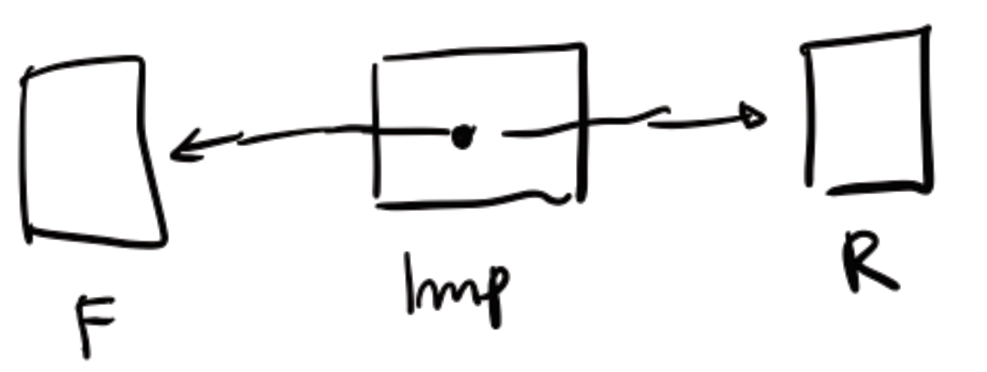
\includegraphics[scale=0.33]{dpcatfig_fir}
    \caption{Evaluation of specific implementations to get functionality and resources spaces.\label{fig:FIR}}
\end{figure}

\paragraph{Systems and components}

Engineers tend to approach complex design problems hierarchically.  The usual
nomenclature refers to \textit{systems} being decomposed into \textit{components}.

\noindent What is a system, and what is a component? Here is a great quote:

\begin{quote}
A system is composed of components; \\
a component is something you understand.\\
---Howard Aiken\footnote{
Howard H. Aiken (1900-1973), creator of the MARK I computer.
Quoted by Kenneth E. Iverson (1920-2004), creator of programming language APL.
Quoted in this paper\cite{that-paper},
  but ultimately sourceless and probably apocryphal.}
\end{quote}

The first part of the quote, "A system is composed of components", is plain as day as much as
it is tautological. We could equally say: "A system is partitioned in parts".

The second part, "a component is something you understand", is the insightful part: We call
"system" what is not obvious to understand, even if we understand all its components
separately.

Whether something can be considered a component, an indivisible atom in the theory, depends on the context.
%
% This definition is, of course, an anthropocentric definition, as it is a
% limitation of the human mind, related to the amount of neurons in the brain. It
% also depends on what exactly is the task at hand with which we are confronted.


\paragraph{Interfaces and interconnection}

Components are \emph{interconnected} to create a system.
This implies that we have defined the \emph{interfaces} of components, which
have the dual function of delimiting when one component ends and another begins,
and also to describe exactly what is the nature of their interaction.

In this paper, we will present a formalism in which the functionality and resources
are the interfaces used for interconnection: Two components are connected
if the resources required by the first correspond to the functionality
provided by the second.




\paragraph{Abstraction}

By \emph{abstraction}, one usually means that it is possible to ``zoom out'',
in the sense that a system of components can be seen as a component itself,
which can be part of larger systems.


\paragraph{Compositionality}

A \emph{compositional} property is a property that is preserved by interconnection and abstraction; assuming each component in a system satisfies that property, also the system as a whole satisfies the property.

\begin{example}
One can compose two electronic circuits by joining their terminals to obtain
another electronic circuit. We would say that the property
of being an electronic circuit is compositional.
\end{example}



\subsection{Queries in design}

\paragraph{Design Queries} The design queries we will present throughout this paper are the following:
\begin{compactitem}
\item Given a certain functionality, find the minimal resources that can realize it, or provide a proof that there are none.
\item Given certain resources, find the maximal functionality that can be realized, or provide a proof that there are none.
\item \todo{...} 
\end{compactitem}




\clearpage
% How things transform
% !TEX root = ../CategoricalCoDesign.tex
\section{Thinking about how things transform into each other}

\subsection{Category theory helps reasoning about interfaces and transformations}
\todo{Arrows should agree with profunctors notation}

We argue that all the concepts of formal engineering design discussed in the
previous section can be naturally described in the language of category theory.

We will start with a simple example.

In an electric car, electric power is turned by the engine into rotational
motion of the axle, and then the rotational motion is converted into
translational motion by the wheels and their friction with the road.

In this simple setting, we can identify the key systems and subsystems: Car,
engine, axle, wheels, and road.

We can identify the functionality/resources of interest as: Electric
power, rotational motion, and translational motion. Note that each of these quantities
plays a dual role: For example, the rotational motion is something which is
produced by the motor, so it is a functionality for the motor, while it
is a resource for axle/wheels, because they need it to provide translational motion.

For a first qualitative description of the scenario, we might choose to just
keep track of what functionality/resource is converted into what.

For this qualitative description, we can draw a diagram in which each resource
is a point (\cref{fig:e1}).

\begin{figure}[h!]
    \centering
    \includesag{30_dpcatfig_e1}
    \caption{\label{fig:e1}}
\end{figure}

Furthermore, we can draw an arrow between two resources if we can obtain one
from the other. In the example, we have described how power becomes rotational
motion (arrow $\mathsf{converter}$) and how rotational motion becomes translational motion
(arrow $\mathsf{wheel}$) (\cref{fig:e2}).

\begin{figure}[h!]
    \centering
    \includesag{30_dpcatfig_e2}
    \caption{\label{fig:e2}}
\end{figure}

In this representation, the arrows are the components of the system.
We will learn how to compose these arrows according to the rules of category theory.

If we use the semantics that an arrow from resource $X$ to resource $Y$ means ``Having $Y$ is
enough to obtain $X$'', then, since $Y$ is enough for $Y$, we can add a self-loop for each
resource (\cref{fig:e3}). We will call the self-loops \emph{identities} (\cref{fig:e3}).

\begin{figure}[h!]
    \centering
    \includesag{30_dpcatfig_e3}
    \caption{\label{fig:e3}}
\end{figure}

Furthermore, we might consider the idea of composition of arrows: if from $Y$ we
can get $X$ and from $Z$ we can get $Y$, then from $Z$ we can get $X$. In our
example, if the arrows $\mathsf{converter}$ and $\mathsf{wheel}$ exist, then also the arrow ``$\mathsf{converter}$ then $\mathsf{wheel}$''
exists~(\cref{fig:e4}).


\begin{figure}[h!]
    \centering
    \includesag{30_dpcatfig_e4}
    \caption{\label{fig:e4}}
\end{figure}


A ``category'' is nothing more than this: It is an abstract mathematical
structure whose two primitive notions are objects and arrows between objects.
The following is the formal definition.

\begin{shaded}
\begin{definition}[Category] \label{def:categorymain}
A \emph{category} $\CatC$ is defined by describing four components: the
category's \emph{objects}, the category's \emph{morphisms},
the \emph{identities} and the \emph{composition operations}. More precisely,
a category consists of:
\begin{compactenum}
\item \emph{Objects}: A collection $\ObC$, whose elements are called \emph{objects}.
\item \emph{Morphisms}: For every pair of objects $X, Y\in\ObC$, there is
a way to define the set $\HomC(X, Y)$, which is called the ``hom-set from
$X$ to $Y$''. The elements of this set are called \emph{morphisms}.
\item \emph{Identity morphism}:  For each object $X$, there is
an element $\id_X \in \HomC(X,X) $ which is called \emph{the identity
morphism in $X$}.
\item \emph{Composition operation}: There is a way to define the composition
of two morphisms. Given a morphism $f \in  \HomC(X,Y) $ and a morphism $g \in \HomC(Y, Z)$, then
there exists a morphism $f\then g$ in $\HomC(X, Z)$.

In addition, there are two properties that must hold:

\begin{compactenum}
    \item Unitality: For a morphism $f\in\Hom(X,Y)$: 
    \begin{equation}
        \id_X \then f=f \then \id_Y.
    \end{equation}
    \item Associativity: The composition is associative, in the sense that for $f\in \HomC(X,Y)$, $g\in \HomC(Y,Z)$, and $h\in \HomC(Z,W)$:
    \begin{equation}
        (f\then g)\then h= f \then (g \then h).
    \end{equation}
\end{compactenum}

\end{compactenum}
\end{definition}
\end{shaded}



\AC{ Given that this is the first example of a category, let's list explicitly
the category that we are using. (wheels, converters, energy, etc.) }

The properties of a category allow us to save some ink in the drawing the
corresponding graph:
\begin{compactitem}
\item We do not need to draw the identity arrows from one object to itself, because they always exist. (However, we will see how there might be multiple such loops.)
\item  Whenever there are arrows $A\to B \to C$, we will not need to draw the arrows composition, because it always exists.
\end{compactitem}

With these conventions, we can just draw the arrows~$f$ and~$g$ in the diagram,
and the rest of the diagram is implied (\cref{fig:e5}). Particularly, this example corresponds to the category $\CatC$ specified by 
\begin{itemize}
    \item $\Ob_\CatC=\{\text{electric power},\text{rotational motion},\text{translational motion}\}$.
    \item E.g., we have morphisms $\mathsf{converter}$, $\mathsf{wheel}$, and $\mathsf{wheel}\text{ then }\mathsf{converter}$.
\end{itemize}

\begin{figure}[h!]
    \centering
    \includesag{30_dpcatfig_e5}
    \caption{\label{fig:e5} The grey arrows are implied by the properties
    of a category.}
\end{figure}

\todo{move the following to the currency subsection. Check the direction of the arrows!}  

We can slightly expand this example by noting the inverse transformations. In an electric car
it is possible to regenerate power; that is, we can obtain rotational motion of the wheels from
translational motion (via $\mathsf{move}$), and then convert the rotational motion into electric
power (via $\mathsf{dynamo}$)~(\cref{fig:e6}).

\begin{remark}
We denote map composition in a somewhat unusual way---sometimes preferred by category-theorists and computer scientists---namely in \emph{diagrammatic order}. That is, given $f\colon A\to B$ and $g\colon B\to C$, we denote their composite by $(f\then g)\colon A\to C$, pronounced ``$f$ then $g$'' rather than the more typical $g\circ f$ (``$g$ after $f$'').

Composition of maps is unital and associative: for any $f\colon A\to B$, $g\colon B\to C$, and $h\colon C\to D$, we have
\begin{equation}
(\id_A\then f)=f=(f \then \id_B)\qquad\text{and}\qquad f\then (g\then h)=(f\then g)\then h.
\end{equation}
\end{remark}

\begin{figure}[h!]
    \centering
    \includesag{30_dpcatfig_e6}
    \caption{\label{fig:e6}}
\end{figure}

These arrows are not necessarily the same arrows as before; there might be different processes
involved.

\begin{figure}[h!]
    \centering
    \includesag{30_dpcatfig_e7}
    \caption{\label{fig:e6-together}}
\end{figure}

Given the semantics of the arrows, all compositions of arrows exist, even if they are not drawn
explicitly. For example, we can consider the composition~$f\then g \then k \then h$, which
converts electric power into rotational motion into translational motion, then back to
rotational motion and electric power. This is an arrow that has the same head and tail as the
identity on electrical power~(\cref{fig:e8}). However, the arrows are not necessarily the same. In fact, we know that if these are physical systems, there will be some loss for the many conversions.

\begin{figure}[h!]
    \centering
    \includesag{30_dpcatfig_e8}
    %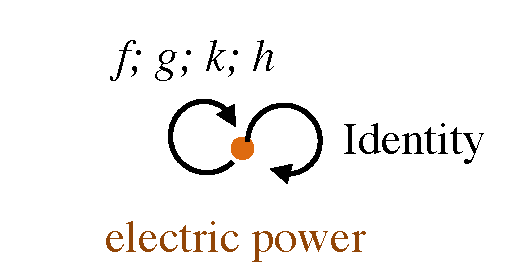
\includegraphics[scale=0.33]{dpcatfig_e8}
    \caption{\label{fig:e8}}
\end{figure}

In fact, it is important to recognize that there might be two or more distinct
arrows between two resources~(\cref{fig:e9}). Each arrow between $X$ and $Y$ represents a different way  to obtain~$X$ from~$Y$. This is what will make category theory powerful enough to reason about design.


\begin{figure}[h!]
    \centering
    \includesag{30_dpcatfig_e9}
    \caption{\label{fig:e9}}
\end{figure}

The directionality of the arrows is also important. While the convention of
which resource is the tail and which the head is just a typographic convention,
it might be the case that we know how to convert one resource into another, but
not vice versa.

\cref{fig:e10} shows an example of a diagram that describes a process which is definitely
not invertible.

\begin{figure}[h!]
    \centering
    \includesag{30_dpcatfig_e10}
    \caption{\label{fig:e10}}
\end{figure}
\subsection{The currency category}
\todo{For later - this will be more discursive. Definitions can be less formal. Symbols too heavy.
Will put nice pictures.}
\AC{I think here we can go to the incremental step of describing a category
in which the resources are isomorphic to real numbers. Before, we say
that fghk is not the identity, but really, if the resources are bool then fghk=identity.}
In this section, we consider as an example the category of currency exchangers $\mathbf{Curr}$. To introduce what currencies are, we need the notion of units.
\begin{definition}[Real with units]
    Define $\mathbb{R}_\mathsf{g}$ to be the set of real numbers $\mathbb{R}$ with unit $\mathsf{g}$. Given $\unit[p]{\mathsf{a}} \in \mathbb{R}_\mathsf{a}$ and $\unit[q]{\mathsf{b}}\in \mathbb{R}_\mathsf{b}$, define
    \begin{equation}
    \begin{aligned}
    \cdot \colon \mathbb{R}_\mathsf{a} \times \mathbb{R}_\mathsf{b} &\to \mathbb{R}_\mathsf{ab}\\
    \tup{\unit[p]{\mathsf{a}},\unit[q]{\mathsf{b}}}&\mapsto r\coloneqq \unit[p\cdot q]{\mathsf{ab}}.
    \end{aligned}
    \end{equation}
    Furthermore, note that two objects can be summed if and only if they share the same units. Note that from now on we will say $p\in \mathbb{R}_\mathsf{g}$ to mean $\unit[p]{\mathsf{g}}$, $p\in \mathbb{R}$.
\end{definition}

Consider two currencies, $\mathsf{C,D}$. A currency exchanger from $\mathsf{C}$ to $\mathsf{D}$ can be expressed as a pair $\tup{a,b}$, $a\in {\mathbb{R}_{>0}}_ {\frac{\mathsf{D}}{\mathsf{C}}}$ and $b\in {\mathbb{R}_{\geq 0}}_ {\mathsf{D}}$. The pair specifies an affine function of the form
\begin{equation}
        \begin{aligned}
        \mathsf{CE}\colon \mathbb{R}_\mathsf{C}&\to \mathbb{R}_\mathsf{D}\\
        \unit[p]{\mathsf{C}}&\mapsto \unit[q]{\mathsf{D}} \coloneqq a\cdot \unit[p]{\mathsf{C}} -b,
        \end{aligned}
    \end{equation}
   where $a$ represents the exchange rate from $\mathsf{C}$ to $\mathsf{D}$, and $b$ represents the fixed commission of the currency exchanger. Note that one can define the identity currency exchanger, $\tup{1,0}$, which is equivalent to not change the money. As an example, consider three currency exchange companies $\mathsf{ExchATM}$, $\mathsf{MoneyLah}$, and $\mathsf{Frankurrencies}$, which operate on several currencies (\cref{tab:currencycompanies}).
\begin{table}[h]
    \centering
    \begin{tabular}{c|c|c|c}
         operation name& details &$a$ (exchange rate)&$b$   (fixed commission)  \\
         $A$&USD to CHF&\unitfrac[0.95]{CHF}{USD}&\unit[2.0]{CHF}\\
         $B$&CHF to USD&\unitfrac[1.05]{USD}{CHF}&\unit[1.5]{USD}\\
         $C$&USD to SGD&\unitfrac[1.40]{SGD}{USD}&\unit[1.0]{SGD}    \end{tabular}\\[+5pt]
         \begin{tabular}{c|c|c|c}
         operation name& details &$a$ (exchange rate)&$b $ (fixed commission)  \\ $D$&USD to CHF&$\unitfrac[1.0]{CHF}{USD}$&\unit[1]{CHF}\\
         $E$&SGD to USD&\unitfrac[0.72]{USD}{SGD}&\unit[3.0]{USD}
    \end{tabular}\\[+5pt]
    \begin{tabular}{c|c|c|c}
         operation name& details &$a$ (exchange rate)&$b $ (fixed commission)  \\
        $F$& EUR to CHF&\unitfrac[1.2]{CHF}{EUR}&\unit[0]{CHF}\\
        $G$& CHF to EUR&\unitfrac[1.0]{EUR}{CHF}&\unit[1]{EUR}
    \end{tabular}
    \caption{Three currency exchange companies operating different currencies.
    }
    \label{tab:currencycompanies}
\end{table}

We can represent this information as a graph, where the nodes are the currencies and the edges are particular exchange operations (\cref{fig:currencygraph}).

\begin{figure}[h]
\begin{center}
    \begin{tikzcd}[column sep = 5cm, row sep = 3cm]
    \text{USD}\arrow[bend left=20, r,"A"]\arrow[bend right=20, r,"D",swap] 
    \arrow[d,bend left=20,"C"]
    &\text{CHF}
    \arrow[d,bend left=20,"G"]
    \arrow[l,"B"]\\
    \text{SGD}\arrow[u,bend left=20,"E"]&
    \text{EUR}
    \arrow[u,bend left=20,"F"]
    \end{tikzcd}
\end{center}
\caption{Three currency exchange companies operating different currencies as a graph \label{fig:currencygraph}}
\end{figure}

The graph representation seems enough to describe this as a category, where the objects are the currencies (USD,CHF,EUR, and SGD), the morphisms are the different exchange operations, and the identity morphisms are identity currency exchangers. However, to properly define this category, we need to define composition and prove that the category is closed with respect to it. Given three currencies $\mathsf{X,Y,Z}$, a currency exchanger $\tup{a,b}$ from $\mathsf{X}$ to $\mathsf{Y}$, and a currency exchanger $\tup{c,d}$ from $\mathsf{Y}$ to $\mathsf{Z}$, one can define their composition as
\begin{equation}
\begin{aligned}
\label{eq:currencycomp}
    \tup{a,b}\then \tup{c,d}&=\tup{c\cdot a,c\cdot b+d}\\
    &=\tup{e,f}.
\end{aligned}
\end{equation}
Note that the result of the composition of currency exchangers is a currency exchanger: This is closure. Finally, we need to check unitality and associativity for composition. Given a currency exchanger $\tup{a,b}$ from $\mathsf{X}$ to $\mathsf{Y}$ one has
\begin{equation}
    \begin{aligned}
    \tup{1,0}\then \tup{a,b}&=\tup{a,b}\then \tup{1,0}\\
    &=\tup{a,b},
    \end{aligned}
\end{equation}
which is unitality. Furthermore, given a currency exchanger $\tup{c,d}$ from $\mathsf{Y}$ to $\mathsf{Z}$ and a currency exchanger $\tup{e,f}$ from $\mathsf{Z}$ to $\mathsf{W}$, one has
\begin{equation}
    \begin{aligned}
    (\tup{a,b}\then \tup{c,d})\then \tup{e,f}&=\tup{a,b}\then( \tup{c,d}\then \tup{e,f})\\
    &=\tup{eca, ecb+ed+f},
    \end{aligned}
\end{equation}
which is associativity.
We are now ready to properly define the category of currency exchangers $\mathbf{Curr}$.

\begin{definition}[Category of currencies]
    The category of currencies $\mathbf{Curr}$ is specified by:
    \begin{compactenum}
        \item \emph{Objects:} $\Ob_\mathbf{Curr}$ is a collection of currencies.
        \item \emph{Morphisms:} Given two currencies $\mathsf{C},\mathsf{D}\in \Ob_{\mathbf{Curr}}$, morphisms between them are currency exchangers $\tup{a,b}$ from $\mathsf{C}$ to $\mathsf{D}$. 
        \item \emph{Identity morphism:} Given an object $C\in \Ob_\mathbf{Curr}$, the identity morphism is given by the currency exchanger $\tup{1,0}$.
        \item \emph{Composition of morphisms:} The composition of morphisms is given by composition of currency exchangers.
    \end{compactenum}
\end{definition}

The category Curr represents the set of all possible currency exchangers that could
ever exist. However, in this set there would be very irrational agents. For example, there is a currency exchanger that given 1 USD, will give you back 2 USD, or even not giving you back any money. This highlights a recurring topic: often mathematicians will be happy to define a broader category of objects, while, in practice, the engineer will find himself thinking about a more constrained set of objects. Particularly, one would like to find the best conversions, which can be expressed as \emph{pareto fronts}, since they are given as tuples $\tup{a,b}$. To do so, one only needs to iterate a finite number of times, since the optimal path (conversion morphism), if such a morphism exists, will never pass through the same currency more than once. This is valid if we assume the action of converting back and forth the same currency to have a cost (through the commission) different from 0. To see this, consider three currencies $\mathsf{A,B,C}$, a currency exchanger from $\mathsf{A}$ to $\mathsf{B}$  $\tup{a,b}$, a currency exchanger from $\mathsf{B}$ to $\mathsf{C}$ 
$\tup{c,d}$, and a currency exchanger from $\mathsf{C}$ to $\mathsf{A}$ $\tup{e,f}$. The composition of the currency exchangers reads:
\begin{equation}
\tup{\underbrace{eca}_{\diamond}, \underbrace{ecb+ed+f}_{\star}}
\end{equation}
Assuming $e=a^{-1}$ (i.e., an exchange rate direction is not more profitable than the other), $\star\neq 0$, because of the commissions. This shows that there are multiple morphisms from $\mathsf{A}$ to $\mathsf{A}$, and that the identity morphism is the most convenient one.


\AC{(Note, don't write: if bias is 0, then take the log of conversion rates, and they add: solve using Dijkstra.)}





\clearpage
% How things connect
% !TEX root = ../CategoricalCoDesign.tex
\section{Thinking about how things connect to each other}
The $\mathbf{Curr}$ category was a good example of how one can use category theory to think about things transform into each other. In this section, we want to think about how things connect to each other.
\subsection{Trekking}
\label{sec:trekking}
Consider geographical locations expressed through coordinates $\tup{x,y}\in \mathbb{R}^2$. Furthermore, consider a map $\mathsf{alt}$ which, for a known place, returns its altitude (assuming smooth terrain):
\begin{equation}
    \begin{aligned}
    \mathsf{alt}\colon \mathbb{R}^2&\to \mathbb{R}_{\geq 0}\\
    \tup{x,y}&\to a.
    \end{aligned}
\end{equation}
Furthermore, consider a human which can traverse trails with a maximum inclination of $\alpha>0$. We can think about this as a category (call it $\mathbf{trek}$), where objects are geographical locations $\tup{x,y}\in \mathbb{R}^2$ and morphisms are paths between them. The identity morphism for each location consists of the trivial path (i.e. not moving), and composition is given by paths concatenation. We can now think of the aforementioned human, willing to go from a location $\tup{x,y}$ to a location $\tup{v,w}$. Finding a path consists of finding at least a morphism in $\Hom_\mathbf{trek}(\tup{x,y},\tup{v,w})$ satisfying the condition on the maximum inclination $\alpha$. We can make the notion of geographical locations and paths more formal, by defining categories from graphs.

\todo{Allow asymmetric bounds for inclincation (maybe you can go up a 50\% inclination, but it would be to risky to go down). Then we have a nice example of a non-symmetryc category }

\todo{Eventually, make an example by taking altimetry of a famous zone, and compute reachability paths from certain points.}


\subsection{Mobility}
Consider now the example of mobility. For a specific mode of transportation, say a car, we can define a graph $G_\mathrm{c}=(V_\mathrm{c},A_\mathrm{c},s_\mathrm{c},t_\mathrm{c})$, where $V$ represents geographical locations that the car can reach in a city and $A_\mathrm{c}$ represents the paths it can take (e.g. roads). Similarly, consider a graph $G_\mathrm{s}=(V_\mathrm{s},A_\mathrm{s},s_\mathrm{s},t_\mathrm{s})$, representing the subway system of a city, with stations $V_\mathrm{s}$ and lines going through paths $A_\mathrm{s}$. In the following, we want to express intermodality, i.e. someone reaching a certain intermediate location on a car and then deciding to take the subway to reach the final destination. By considering the graph $G=(V,A,s,t)$, with $V=V_\mathrm{c}\cup V_\mathrm{s}$ and $A=A_\mathrm{c}\cup A_\mathrm{s}$, one obtains the desired intermodality. The arising graph can be seen as a new category, with objects $V$ and morphisms $A$.
\begin{example}
Consider the car category with $V_\mathrm{c}=\{\mathsf{ETHZ},\mathsf{Oerlikon},\mathsf{Uetliberg}\}$ and arrows as in~\cref{fig:carcat}.
\todo{Concrete examples: put names for the arrows.}

\begin{figure}[h!]
\begin{center}
\includesag{30_carcategory}
\end{center}
\caption{Car category. \label{fig:carcat}}
\end{figure}

Furthermore, consider the subway category with $V_\mathrm{s}=\{\mathsf{ETHZ},\mathsf{Oerlikon},\mathsf{Seebach},\mathsf{Dietlikon}\}$ and arrows as in~\cref{fig:subcat}.

\todo{Use different modality: Zurich has no subway}

\begin{figure}[h!]
\begin{center}
\includesag{30_subwaycat}
\end{center}
\caption{Subway category. \label{fig:subcat}}
\end{figure}
The union of the two, which we call the \emph{intermodal graph}, can be represented as a graph, with \textcolor{red}{red} arrows for the car network and \textcolor{blue}{blue} arrows for the subway network (\cref{fig:intermodal}).

\begin{figure}[h!]
\begin{center}
\includesag{30_intermodal}
\end{center}
\caption{Intermodal graph. \label{fig:intermodal}}
\end{figure}
\end{example}

\todo{In the intermodal graph, show some morphisms that are "mixed" because they are the composition o two modalities. }


This concept is formalized with the union of categories
\begin{shaded}
\begin{definition}[Union of categories]
Given two categories $\CatC,\CatD$, one can create the \emph{union} $\Cat{E}$ of the two, which is specified by:
\begin{compactenum}
\item \emph{Objects:} $\Ob_\Cat{E}=\Ob_\CatC \cup \Ob_\CatD$.
\item \emph{Morphisms:} A morphism $f$ is given by considering the followng. If $f\in \Hom_\CatC(X,Y)$, then $f\in \Hom_\Cat{E}(X,Y)$. If $f\in \Hom_\CatD(X,Y)$, then $f\in \Hom_\Cat{E}(X,Y)$.
\item \emph{Identity morphism:} For any morphism in $\Cat{E}$, the identity morphism remais the same as in the original category.
\item \emph{Composition operation}: The composition of morphisms remains the same.
\end{compactenum}
\end{definition}
\end{shaded}

\subsection{Generating categories from graphs}
What we sketched is the previous sections has deeper roots.
\begin{definition}[Graph]
A \emph{graph} $G=\tup{V,A,s,t}$ consists of a set of vertices $V$, a set of arrows $A$, and two functions $s,t\colon A\to V$, called the \emph{source} and \emph{target} functions, respectively. Given $a\in A$ with $s(a)=v$ and $t(a)=w$, one says that $a$ is an arrow from $v$ to $w$. A path in $G$ is a sequence of arrows such that the target of one arrow is the source of the next. Note that a path of length 1 (one single arrow) from a vertex to itself always exists. We call it \emph{trivial}.
\end{definition}

\begin{shaded}
\begin{definition}[Free category on a graph]
Consider any graph $G=(V,A,s,t)$. One can define the category $\mathbf{Free}(G)$, called the \emph{free category on $G$}. Its objects are the vertices $V$, and its morphisms from $c\in V$ to $d\in V$ are the paths from $c$ to $d$. The identity morphism of an object $c\in V$ is the trivial path at $c$. Composition of morphisms is given by paths' concatenation.
\end{definition}
\end{shaded}


With these two new definitions, we can see that $\mathbf{trek}$ is the free category on a graph with vertices given by geographical locations $\tup{x,y}\in \mathbb{R}^2$ and arrows given by paths between them. Particularly, a valid path $p\colon \tup{x,y}\mapsto \tup{v,w}$ for the vehicle to be able to reach a destination $\tup{v,w}$ from $\tup{x,y}$ can be written as a composition of paths $p_1\then \ldots \then p_n$, where $s(p_1)=\tup{x,y}$ and $t(p_n)=\tup{v,w}$, and
\begin{equation}
    \frac{\mathsf{alt}(t(p_i))-\mathsf{alt}(s(p_i))}{\vert t(p_i), s(p_i)\vert}\leq \alpha, \quad \forall i\in \{1,\ldots, n\},
\end{equation}
where $\vert \tup{x,y},\tup{v,w}\vert$ represents the distance $\sqrt{(v-x)^2+(w-y)^2}$.

\todo{ This part is wrong as written. (why? because you must assure that the inclination is compatible all along the path, not just at the intermediate points. In general paths should be \textbf{continuous} paths for this to work. Morphisms are continuous paths, not finite sequences of points.}


\subsection{The Set category}


\begin{shaded}
\begin{definition}[Category $\Set$]
    The category $\Set$ is defined by:
    \begin{compactenum}
    \item \emph{Objects}: The objects of this category are all sets.
    \item \emph{Morphisms}: The morphisms between any pair of sets $X, Y$
    are maps from $X$ to $Y$.
    \item \emph{Identity morphism}: The identity morphism for the set $X$
    is the identity function $\text{Id}_X$.
    \item \emph{Composition operation}: The composition operation is function
    composition.
    \end{compactenum}
\end{definition}
\end{shaded}

Note that $\Set$ is precisely defined by the four points above. However, there are categories where objects are sets which differ from $\Set$ in the morphisms, as outlined in the following example.
\begin{example}
\label{ex:hasseinclusion}
Given a set $X=\{a,b,c\}$, consider its power set $\powerset{X}$. Define sets as the objects of this new category and define the morphisms to be inclusions (\cref{fig:powersetcat}).
\begin{figure}[h!]
\begin{center}
\includesag{40_dpcatfig_power}
\end{center}
\caption{Power set as a category. \label{fig:powersetcat}}
\end{figure}
The identity morphism of each set is the inclusion with itself (every set is a subset of itself). Composition is given by composition of inclusions, i.e. if $X\subseteq Y \subseteq Z$, then $X\subseteq Z$.
\end{example}
% Constraints
% !TEX root = ../CategoricalCoDesign.tex
\subsection{Thinking about specifity of constraints}
\begin{shaded}
\begin{definition}[Subcategory]
\label{def:subcategory}
	Given a category $\Cat{A}$, a \emph{subcategory} $\Cat{B}$ consists of a subcollection of the collection of objects and morphisms of $\Cat{A}$ such that:
	\begin{enumerate}[(i)]
	\item If a morphism $f \colon x\to y$ is in $\Cat{B}$, then so are the objects $x$ and $y$.
	\item If the morphisms $f\colon x\to y$ and $g\colon y\to z$ are in $\Cat{B}$, then so is their composite $f\then g\colon x\to z$.
	\item If $x$ is in $\Cat{B}$, then so is the identity morphism $\text{Id}_x$.
	\end{enumerate}
\end{definition}
\end{shaded}

\begin{lemma}
    $\mathbf{Curr}$ is a subcategory of $\Set$.
\end{lemma}

\begin{proof}
    We need to check the conditions presented in \cref{def:subcategory}.
    \begin{enumerate}[(i)]
        \item If a morphism of $\Set$ $f\colon X\to Y$ is in $\mathbf{Curr}$, it means automatically that both $X$ and $Y$ are singletons, containing currencies, and that $f$ can be represented as a currency exchanger.
        \item If morphisms of $\Set$ $f\colon X\to Y$ and $g\colon Y \to Z$ are in $\mathbf{Curr}$, then from (i) we know that $X,Y,Z$ are as well, that $f,g$ are currency exchangers, and that we can write their composition.
        \item If $X$ is in $\mathbf{Curr}$, then the identity morphism $\text{Id}_X$ in $\Set$ can be written as an identity currency exchanger.
    \end{enumerate}
\end{proof}
\clearpage
% Resource composition
% !TEX root = ../CategoricalCoDesign.tex
\section{Thinking about resource composition}
\subsection{Products}
Is ``$X \times Y$'' the same as ``$Y \times X$''?
It depends on the context. Intuitively, for our categories of resources, we would not make a distinction
between ``having $X$ and $Y$'' and ``having $Y$ and $X$''.
However, there are contexts in which this is not valid. For example, if we are
using $X \times Y$ to mean that we will have the resource $X$ today, and the
resource $Y$ tomorrow, then $Y \times X$ would not be the same as $X \times Y$.

In the contexts in which this symmetry holds, we call the category ``symmetric''.
\AC{I will make this more precise later.}
The word ``symmetric'' is well suited, because to say that the two objects are equivalent,
or ``isomorphic'', we can postulate that we always have a way to get
``$X \times Y$'' starting from ``$Y \times X$'' and viceversa. In the diagram, this is depicted
by the two arrows that connect them~(\cref{fig:e17}).

\begin{figure}[h!]
    \centering
    \includesag{30_dpcatfig_e17}
    \caption{\label{fig:e17}}
\end{figure}

Consider the following example: To generate motion, one needs \emph{both} an engine \emph{and} some fuel.

We can consider ``motion'', ``fuel'', and ``engine'' as resources and draw them as points (\cref{fig:e11}).

\begin{figure}[h!]
    \centering
    \includesag{30_dpcatfig_e11}
    %
\includegraphics[scale=0.33]{dpcatfig_e11}
    \caption{\label{fig:e11}}
\end{figure}

However, it is not clear how to represent the arrow corresponding to
``fuel + engine = motion'', because arrows only have one head and
one tail.

One clean way to formalize this is to expand the objects in the category,
by postulating that,
if two resources~$X$ and~$Y$ exist, then there exists also the
resource ``$X$ \emph{and} $Y$''.


In our example, we can postulate the existence of an object ``engine \emph{and}
fuel'' and then draw the arrow from it to motion (\cref{fig:e13}).

\begin{figure}[h!]
    \centering
    \includesag{30_dpcatfig_e13}
    \caption{\label{fig:e13} 
    \AC{There should be 3 dots: "engine", "fuel", "engine and fuel"}
    }
\end{figure}

We call this construction ``product'' because it is equivalent to
the Cartesian product of sets (\cref{def:cartesian-product}).

\begin{definition}[Cartesian product]
\label{def:cartesian-product}
   Given two sets $A,B$, their \emph{cartesian product} is denoted $A\times  B$
   and defined as 
   \begin{equation}
       A\times  B=\{ \tup{a,b}\mid a\in A\text{ and } b\in B\}.
   \end{equation}
\end{definition}

\begin{figure}[h!]
    \centering
    \includesag{50_cartesian_product}
    \caption{Example of cartesian product of two sets.\label{fig:cartesian-product}}
\end{figure}

Given the Cartesian product of two sets, we can define two \emph{projection maps} $\pi_1$
and $\pi_2$, which, given an element of the product, will return the first or the second
element:
\begin{equation}
\begin{aligned}
    \pi_1(\tup{a,b}) &= a,\\
    \pi_2(\tup{a,b}) &= b.
\end{aligned}
\end{equation}

In our case, we would be able to say that, given both $\mathsf{resource}_1$ and $\mathsf{resource}_2$,
we can recover resource1 and resource2 separately~(\cref{fig:resource-product}).

\begin{figure}[h!]
    \centering
    \includesag{30_recover}
    \caption{Two projection maps \label{fig:resource-product}.}
\end{figure}


Later, we will see other examples of products, such as the products of partially ordered sets.
All these products are an instance of a more generic concept of product that exists in category
theory.  The formal definition is below.
 
\begin{shaded}
\begin{definition}[Categorical Product]
The \emph{product} of two objects $A$ and $B$ is an object $A \times B \in \CatC$ together with canonical morphisms $\pi_A \colon A \times B \to A$ and $\pi_B \colon A \times B \to B$, such that, given any $X \in \CatC$ and morphisms $f \colon X \to A, g \colon X \to B$, there exists a \emph{unique} morphism $(\prodMap{f}{g}) \colon X \to A \times B$ such that $f = (\prodMap{f}{g})\then \pi_A$ and $g=(\prodMap{f}{g})\then \pi_B$.
\end{definition}
\end{shaded}

The formulation, slightly technical, hints at uniqueness properties or ``universality''.
The definition implies that if a product exists, then it is unique, in the sense
that all the admissible products can be derived from each other. Therefore, when
presented with a new category, one can guess what construction might be the product, and check
the definition to make sure that it is indeed \emph{the} product.
\clearpage
% Alternatives
% !TEX root = ../CategoricalCoDesign.tex
\section{Thinking about alternatives}
\subsubsection{Coproduct}

There exists a dual notion to ``product'' that is called ``coproduct''. Here is the motivation in the context of engineering design.
Suppose that we are considering a hybrid car that contains two engines: An
electric engine and an internal combustion engine. Both can produce motion, from
different sources of energy. The electric engine uses electric energy; the
internal combustion engine uses gasoline. The situation is as in \cref{fig:e16a}.

\begin{figure}[h!]
    \centering
    \includesag{30_dpcatfig_e14}
    %\includegraphics[scale=0.33]{dpcatfig_e14}
    \caption{\label{fig:e16a}}
\end{figure}

From this we would like to conclude that we can obtain motion
from \emph{either} gas \emph{or}
electric energy~(\cref{fig:e16b}).

\begin{figure}[h!]
    \centering
    \includesag{30_dpcatfig_e15}
    %\includegraphics[scale=0.33]{dpcatfig_e15}
    \caption{\label{fig:e16b}}
\end{figure}

To define the idea of ``\emph{either gas \emph{or} electric energy}'' we can
refer to the idea of disjoint union of sets (\cref{def:disjoint-union}). The
disjoint union of two sets is a set that contains two complete copies of the two
sets. If an element is contained in both sets, there will be two distinct copies
in the disjoint union.

\begin{definition}[Disjoint union]
\label{def:disjoint-union}
    The \emph{disjoint union} of two sets $A$ and $B$ is denoted $A + B$
    and it is defined as
    \begin{equation}
        A + B=\{\tup{1,a}\mid a\in A\}\cup\{\tup{2,b}\mid b\in B\}.
    \end{equation}
\end{definition}


\begin{figure}[h!]
    \begin{center}
    \includesag{30_disjoint_union}
    \end{center}
    \caption{Example of disjoint union.}
\end{figure}


We can define the disjoint union of a set with itself; this is equivalent
to having two distinct copies of the set~(\cref{fig:disjointself}).

\begin{figure}[h!]
\begin{center}
\includesag{30_disjoint_union_self}
    \caption{Disjoint union of a set with itself \label{fig:disjointself}.}
\end{center}
\end{figure}

The dsjoint union is a particular instance of the notion of ``coproduct''.
The following definition is the generic definition of coproducts for an arbitrary category.

\begin{shaded}
\begin{definition}[Coproduct]
Let $\CatC$ be a category and let $A, B \in \CatC$ be objects. The \emph{coproduct} of $A$ and $B$ is an object $A \sqcup B \in \CatC$ together with two \emph{inclusion maps} $\iota_A \colon A \to A \sqcup B $ and $\iota_B \colon B \to A  \sqcup B $, such that, given any $X \in \CatC$ and morphisms $f\colon  A \to X, g \colon B \to X$, there exists a \emph{unique} morphism $(\coprodMap{f}{g}) \colon A \sqcup B \to X$ such that $f = \iota_A\then (\coprodMap{f}{g})$ and $g = \iota_B \then (\coprodMap{f}{g})$.
\end{definition}
\end{shaded}

\begin{example}

The two inclusion maps for the disjoint union are $\iota_1\colon A \to A + B$ and $\iota_2\colon B \to A + B$, defined as:
\begin{equation}
\begin{aligned}
    \iota_1(a) &= \tup{1, a},\\
    \iota_2(b) &= \tup{2, b}.
\end{aligned}
\end{equation}

The map $\coprodMap{f}{g}$ for the disjoint union is
\begin{equation}
\begin{aligned}
    \coprodMap{f}{g} \colon  A + B &\to X \\
    y &   \mapsto
    \begin{cases}
        f(y), & \text{if } y \in A, \\
        g(y), & \text{if } y \in B.
    \end{cases}
\end{aligned}
\end{equation}
\end{example}

\todo{figure that shows the injections: from ``gas'' I can get ``gas or electricity''.}


\todo{collocate it well}
$X \sqcup Y$ is different from $Y \sqcup X$, but the two are isomorphic~(\cref{fig:e16}).

\begin{figure}[h!]
    \centering
    \includesag{30_dpcatfig_e16}
    \caption{\label{fig:e16}}
\end{figure}

\clearpage
% Tradeoffs
% !TEX root = ../CategoricalCoDesign.tex
\section{Thinking about tradeoffs}
So far, the discussion has been purely qualitative: While we discussed how
categories can describe the way that one resource can be turned into another,
this kind of modelling did not allow for quantitative statements. For example, it
is good to know that we can obtain motion from electric power, but, how fast can
we go with a certain amount of power?

To achieve a quantitative theory, we need to introduce two aspects.
First, we need to specify various degrees of resources and functionality.
For this, we will use the idea of partial orders.
Second, we need to describe how these various degrees map to each other.
For this, it is important to describe monotone maps.

\AC{ Why do we need the posets? make a concrete example. E.g. We can
have two resources, "time" and "money" that we care about when we prepare the cakes.

Introduce pareto fronts (antichain, upper sets, lower sets) with relation to
a specific example. }
\subsection{Partially ordered sets}

We will assume that functionality and resources
are \emph{partially-ordered sets} (or \emph{posets}).%


\gray{
Such ordering arise naturally in engineering as criteria for judging whether one design is better or worse than another.\AC{expand}
}

\begin{definition}[Partially ordered set]
    A \emph{partially-ordered set} is a tuple $ \tup{P, \leq}$,
where $P$ is a set (also called the \emph{carrier set}), together with a
relation $\leq$ on $P$ that is reflexive, transitive, and antisymmetric.%
\end{definition}

\todo{Recall definitions of the properties above.}



\begin{example}[Singleton poset]\label{ex:singleton}
If a set has only one element, say $\singleton$, then there is a unique order relation on it (\cref{fig:singleton}). We denote the resulting poset again by $\singleton$.
\end{example}
\begin{figure}[h!]
   \centering
   \includesag{40_dpcatfig_singleton}
   \caption{\label{fig:singleton}}
\end{figure}


\begin{example}[Booleans]\label{ex:bool}
The booleans $\Bool$ is a poset with carrier set $\{\true,\false\}$ and the order relation given by $b_1 \leq_\Bool b_2$ iff $b_1 \Imp b_2$, that is, $\false \leq_\Bool \true$. This relation should be familiar from the following table:
\[
\begin{array}{cc|ccc}
a & b & a \leq_\Bool b & a \wedge b & a \vee b \\ \hline
\true&\true&\true&\true&\true\\
\true&\false&\false&\false&\true\\
\false&\true&\true&\false&\true\\
\false&\false&\true&\false&\false
\end{array}
\]
In addition to the operation $\Imp\colon\Bool\times \Bool\to\Bool$, called \emph{implies}, there are also the familiar \emph{and} ($\wedge$) and \emph{or} ($\vee$) operations. Note that $\wedge$ and $\vee$ are commutative ($b\wedge c = c\wedge b$), whereas $\Imp$ is not.
\end{example}

\GZ{
\begin{figure}[h!]
   \centering
   %\includegraphics[scale=0.33]{dpcatfig_boolean}
   \includesag{40_dpcatfig_boolean}
   \caption{\label{fig:boolean}}
\end{figure}}
\AC{The problem with the above figure is that it is not clear what direction is $\leq$. 
Also what direction is $\Rightarrow$.}


\begin{example}[Reals]
The real numbers $\mathbb{R}$ is a poset with carrier $a\in \mathbb{R}$ and order relation given by the usual ordering $r_1 \leq r_2$.
\end{example}


A \emph{Hasse diagram} is a way to visualize a poset by being economical about the arrows that we use. In a Hasse diagram elements are points, and if $a \leq b$ then $a$ is drawn lower than $b$ and with an edge connected to it~(\cref{fig:dpcatfig_hasse}).

\GZ{
Category theory is all about organizing and layering structures. Given systems $A$ and $B$, we say that $A\leq B$ if, whenever $x$ is connected to $y$ in $A$, then $x$ is connected to $y$ in $B$.}


\begin{example}
\label{ex:hasseinclusion}

\AC{I would move this example after Set and do Set + inclusion to give an example
of two categories with same objects but different morphisms}
\GZ{but we don't have a notion of order there, right?}

\GZ{Given a set $X$ consider its power set $\powerset{X}$. We can give it an order by inclusion of subsets. Consider $X=\{a,b,c\}$: its powerset $\powerset{X}$ can be depicted as:}
\begin{center}
\includesag{40_dpcatfig_power}
\end{center}
\end{example}

\begin{figure}[h!]
   \centering
   \includesag{40_dpcatfig_hasse}
   \caption{\label{fig:hasse}}
\end{figure}

\begin{example}[Discrete partially ordered sets]
\label{ex:discreteposet}
{Every set $X$ can be considered as a \emph{discrete poset} $(X,=)$. Discrete posets are represented as collection of points:}
\begin{center}
\includesag{40_discrete}
\end{center}
\end{example}

\AC{Move later}
\begin{definition}[Opposite of a poset]

    The \emph{opposite} of a  poset $\langle A, \leq \rangle $ is the poset $\langle A\op, \leq\op\rangle $ that has the same elements as~$A$ and the reverse ordering.
    For a given~$x \in A$, we use~$x^*$ to represent its corresponding copy in~$A\op$;
    note that~$x$ and~$x^*$ are distinct.
    Reversing the order means that, for all $x,y\in A$,
    \begin{equation}
        x \leq y \quad \Leftrightarrow \quad y^* \leq\op x^*.
    \end{equation}

\end{definition}

\begin{figure}[h!]
   \centering
   \includesag{40_dpcatfig_opposite}
   \caption{\label{fig:opposite}}
\end{figure}


\begin{example}[Credit and debt]
   Let us define the set $\text{USD}=\{\$0.00,\$0.01,\$0.02,\dots\}$
   of all US dollars monetary quantities approximated to the cent.
   From this set we can define two posets:
       $\text{USD}^{+} = \tup{\text{USD}, \leq}$
       and $\text{USD}^{-} = \tup{\text{USD}, \geq}$
       that are opposite of each other.
   If the context is that, given two quantities~$\$1$ and~$\$2$,
   we prefer~$\$1$ to~$\$2$ (for example because it is a cost to pay to acquire a component), then we are working in~$\text{USD}^{+}$,
   otherwise we are working in~$\text{USD}^{-}$ (for example
   because it represents the price at which we are selling our product).

   Traditionally, in double-entry ledger systems, the numbers were not
   written with negative signs, but rather in color: red and black.
   From this convention we get the idioms ``being in the black''
   and ``being in the red''.

\end{example}


\subsection{Staring at Pareto fronts}
\AC{Design = compromise = pareto front.
Draw some pareto front (for continuous, discrete poset) and 
use those diagrams to explain the notions.
All these notions are very graphical.}

\subsubsection{Chains and Antichains} \label{sec:chains-antichains}


\begin{definition}[Chain in a poset]
\label{def:chain}
Given a poset $S$, a \emph{chain} is a sequence of points ${s_i}$ in~$S$ where two successives points are comparable:
\begin{equation}
    i \leq j \Rightarrow s_i \leq s_j.
\end{equation}
\end{definition}

 
\begin{definition}[Antichain in a poset]
\label{def:antichain}
An \emph{antichain} is a subset $S$ of a poset where no elements are comparable. If $a,b \in S$, then $a \leq b$ implies $a=b$.
\end{definition}

We denote the set of antichains of a poset $P$ by $\antichains P$.

\GZ{\begin{example}
Let's consider the poset $\tup{P,\leq}$ where $a\leq b$ if $a$ is a divisor of $b$ and $P=\{1,5,10,11,13,15\}$. A chain of $P$ is $\{1,5,10,15\}$. An antichain of $P$ is $\{10,11,13\}$.
\end{example}

\begin{example}
Consider \cref{ex:hasseinclusion}. Examples of chains are 
\begin{equation}
    \{\varnothing,\{a\},\{a,b\},\{a,b,c\}\}, \quad  \{\varnothing,\{b\},\{b,c\},\{a,b,c\}\}.
\end{equation}

Examples of antichains are
\begin{equation}
    \{\{a\},\{b\},\{c\}\}, \quad \{ \{a,b\},\{a,c\}, \{b,c\}\}.
\end{equation}
\end{example}}

\todo{add here comments, examples and figures}

\subsubsection{Upper and lower sets}

% also called cone
\begin{definition}[Upper set]
\label{def:upperset}An upper set is a subset $U$ of a poset $X$ such
that, if a point is inside, all points above it are inside as well.
In formulas:
\begin{equation}
\text{$U$ is an upperset} \equiv \forall x\in U, \forall y\in X\colon x\leq y \Imp y\in U.
% \begin{prooftree}
%      \AxiomC{x\in U}
%      \AxiomC{x \leq y}
%      \BinaryInfC{y \in U}
%  \end{prooftree}
\end{equation}
\end{definition}

\begin{definition}[Lower set]
\label{def:lowerset}
\todo[inline]{as above}
\end{definition}

\todo[inline]{Examples}

\subsubsection{From antichains to uppersets and viceversa}


\begin{definition}[Upper closure]
\label{def:upperclosure}
Given a point $p$ in a poset $P$, its upper closure $\uparrow p$ is the subset of $P$ that is ``above'' $p$:
    \begin{equation}
        \uparrow p = \{ q\in P \colon p \leq q\}.
    \end{equation}
    The upper closure of a set is the union of the upper closures of its points:
    \begin{equation}
        \uparrow S = \bigcup_{p\in S}\uparrow p.
    \end{equation}
\end{definition}

\AC{And lower closure}

\AC{Equivalently: upper set is closed to upper closure}

\AC{Give the functions that convert one to another and explain the subtletlies.
Example: take ${x\in R : x>0}$ as a poset that is not downward closed.}

\begin{definition}
\label{def:Min}
$\Min \colon \powerset(P) \to \antichains P$ is the monotone map that sends a subset $S$ of a poset to the minimal elements of that subset, i.e., those elements $a \in S$ such that $a \leq b$ for all $b \in S$.
\end{definition}
\AC{this can be empty}
\begin{definition}
\label{def:Max}
$\Max \colon \powerset(P) \to \antichains P$ is the monotone map that sends a subset $S$ of a poset to the maximal elements of that subset, i.e., those elements $a \in S$ such that $a \geq b$ for all $b \in S$.
\end{definition}
\AC{this can be empty}


\todo{Before that, define monotone map, power set notation, power poset relation, antichains relations}


\begin{definition}[Downward closed set]
\label{def:downward-closed-upperset}
An upper set $S$ is downward-closed in a poset $P$ if
\begin{equation}
    S =\, \uparrow \Min S
\end{equation}
The set of downward-closed upper sets of $P$ is denoted $\dcuppersets P$.
\end{definition}

\GZ{
\begin{example}[Upper and lower sets in $\Bool$]
The booleans $\{\false, \true \}$ form a preorder with $\false \leq \true:(\Bool,\leq)$ . The subset $\{\false\} \subseteq \Bool$ is not an upper set, since $\false \leq \true$ and $\true \notin \{\false \}$.	
\end{example}}

\todo{add here comments, examples and figures}
\clearpage
% Posets with more structire
% !TEX root = ../CategoricalCoDesign.tex
\section{Posets with more structure}
In the following, we add some structure to the definition of a poset, by introducing \emph{monoidal posets} and \emph{lattices}.
\subsection{Monoidal posets}
\begin{definition}[Monoidal poset]
\label{def:monoidal_poset}
A \emph{monoidal structure} on a poset $\tup{P,\leq}$ consists of:
\begin{compactenum}
    \item An element $I\in P$, called \emph{monoidal unit}, and
    \item a function $\otimes\colon P\times P\to P$, called the \emph{monoidal product}. Note that we write $\otimes(p_1,p_2)=p_1\otimes p_2$, $p_1,p_2\in P$.
\end{compactenum}
The constituents must satisfy the following properties:
\begin{compactenum}[(a)]
    \item \emph{Monotonicity}: For all $p_1,p_2,q_1,q_2\in P$, if $p_1\leq q_1$ and $p_2\leq q_2$, then $p_1\otimes p_2\leq q_1\otimes q_2$.
    \item \emph{Unitality}: For all $p\in P$, $I\otimes p=p$ and $p\otimes I=p$.
    \item \emph{Associativity}: For all $p,q,r\in P$, $(p\otimes q)\otimes r=p\otimes (q\otimes r)$.
\end{compactenum}
A poset equipped with a monoidal structure $\tup{P,\leq,I,\otimes}$ is called a \emph{monoidal poset}.
\end{definition}

\begin{example}
Consider the real numbers $\mathbb{R}$ with the poset structure given by $\leq$. Consider 0 as monoidal unit and the operation $+\colon \mathbb{R}\times \mathbb{R}\to \mathbb{R}$ as mononidal product. It is easy to see that the conditions of~\cref{def:monoidal_poset} are satisfyied:
\begin{compactenum}[(a)]
    \item If $p_1\leq p_2$ and $q_1\leq q_2$, it is true that $p_1+p_2\leq q_1+q_2$, $p_1,p_2,q_1,q_2\in \mathbb{R}$.
    \item $0+p=p+0=0$, $p\in \mathbb{R}$.
    \item $(p+q)+r=p+(q+r)$, $p,q,r\in \mathbb{R}$.
\end{compactenum}
\end{example}
\subsection{Lattices}
\begin{definition}[Lattice]
\label{def:lattice}
A \emph{lattice} is a poset $\tup{P, \leq}$ with some additional properties:
\begin{compactenum}
    \item Given two points $p, q \in P$, it is always possible to define their least upper bound, called \emph{join}, and indicated as $p \vee q$.
    \item Given two points $p, q \in P$, it is always possible to define their greatest lower bound, called \emph{meet}, and indicated as $p \wedge q$.
\end{compactenum}
\end{definition}

\begin{remark}[Bounded lattices]
If there is a least upper bound for the entire lattice $A$, it is called
the \emph{top} ($\top$). If the greatest lower bound exists it is called the \emph{bottom} ($\bot$). If both a top and a bottom exist, we call the lattice \emph{bounded}, and denote it by $\tup{A,\leq,\vee,\wedge,\bot,\top}$.
\end{remark}

\begin{example}
    In \cref{ex:hasseinclusion} we presented the poset arising from the power set of a set $A$ and ordered via subset inclusion. This is a lattice, bounded by $A$ and by the empty set $\emptyset$. Note that this lattice possesses two (dual) monoidal structures $\tup{\powerset(A),\subseteq,\emptyset,\cup}$ and $\tup{\powerset(A),\subseteq,A,\cap}$.
\end{example}

\begin{example}
Consider the set $\{1,2,3,6\}$ ordered by divisibility. This is a lattice. However, the set $\{1,2,3\}$ ordered by divisibility is not, since 2 and 3 lack a meet (\cref{fig:exlattice}).
\begin{figure}[h!]
\begin{center}
\includesag{40_dpcatfig_exlattice}
\end{center}
\caption{Examples of lattice and non-lattice. \label{fig:exlattice}}
\end{figure}
\end{example}
\clearpage
% Monotonicity
% !TEX root = ../CategoricalCoDesign.tex
\section{Monotonicity is a fact of life}
\subsection{Monotone maps}
\AC{Add some motivation from design. E.g. generalization of "non-decreasing" and "non-increasing" from real numbers to partial orders}
\todo{I would skip the "isomorphism" definition because we can't use it yet. Move to the end}
\begin{definition}[Monotone map]
A monotone map between two posets
$\tup{A, \leq_A}$ and $\tup{B, \leq_B}$ is a map that preserves the ordering, in the sense that 
\begin{equation}
 a \leq_A b \quad \Imp \quad f(a) \leq_B f(b).
\end{equation}

\noindent A monotone map is an \emph{isomorphism} if the other direction
of the implication holds as well:
\begin{equation}
 a \leq_A b \quad \Leftrightarrow \quad f(a) \leq_B f(b).
\end{equation}
\end{definition}
\todo{the below uses "preorder" but we never defined it.}
\begin{remark}
Given a preorder $A$, $\id_A$ is monotone, since for $a_1,a_2\in A$, one has:
\begin{equation}
a_1\leq_A a_2 \Imp a_1=a_1\then \id_A \leq_A a_2\then \id_A = a_2.
\end{equation}
\end{remark}



\begin{example}
In \cref{ex:hasseinclusion} we presented the poset arising from the power set of a set $A=\{a,b,c\}$ and ordered via subset inclusion. The map $\vert \cdot \vert \colon \powerset(A)\to \mathbb{N}$ (cardinality), is a monotone map (\cref{fig:cardinality}).
\begin{figure}[h!]
\begin{center}
\includesag{40_dpcatfig_exmonotone}
\end{center}
\caption{The map from the power set of a set to cardinality is a monotone map. \label{fig:cardinality}}
\end{figure}
\end{example}

\noindent Note that monotonicity is a compositional property.

\begin{lemma}Given three posets $A, B, C$ and two monotone maps $f\colon A
\to B$ and  $g\colon B \to C$, the composite map $f\then g\colon  A \to C$ is
monotone as well.
\end{lemma}
\begin{proof}
Consider $a_1,a_2 \in A$, $b_1,b_2\in B$. We have 
\begin{equation}
\begin{aligned}
        a_1\leq_A a_2 &\Imp f(a_1)\leq_B f(a_2)\\ 
        b_1\leq_B b_2 &\Imp g(b_1)\leq_C g(b_2).
\end{aligned}
\end{equation}
By substituting the above, one has
\begin{equation}
    a_1\leq_A a_2 \Imp (f\then g)(a_1) \leq_C (f\then g)(a_2),
\end{equation}
which is the monotonicity condition for $(f\then g)$.
\end{proof}

\begin{lemma}
Consider a discrete poset $A$ and a poset $B$. Any map $f\colon A\to B$ is monotone.
\end{lemma}
\begin{proof}
Since $A$ is a discrete poset, one has
\begin{equation}
    a_1\leq_A a_2 \iff a_1=a_2.
\end{equation}
Therefore, one has
\begin{equation}
\begin{aligned}
    a_1\leq_A a_2 &\Imp a_1=a_2\\
    &\Imp f(a_1)=f(a_2)\\
    &\Imp f(a_1)\leq_B f(a_2).
\end{aligned}
\end{equation}
\end{proof}
Unless indicated otherwise, in this paper all maps between two posets
are assumed to be monotone or will turn out to be monotone.

\subsection{The category $\Pos$ of posets and monotone maps}
In the previous section, we described a poset as a category, where the objects are elements of the poset and the morphisms are given by the poset order. In this section, we want to lift this concept and describe a category in which the objects are posets themselves, and the morphisms are monotone functions between them. This category is called $\Pos$.

\begin{definition}[Category $\Pos$]
    The category $\Pos$ is defined by:
    \begin{compactenum}
    \item \emph{Objects}: The objects of this category are all posets.
    \item \emph{Morphisms}: The morphisms between any pair of posets $X, Y$
    are the monotone maps from $X$ to $Y$.
    \item \emph{Identity morphism}:  The identity morphism for the poset $X$
    is the identity function $\text{Id}_X$.
    \item \emph{Composition operation}: The composition operation is function
    composition.
    \end{compactenum}
\end{definition}

Occasionally we will write $f \colon A \to_{\Pos} B$ to emphasize that a monotone map between posets is a morphism in the category of posets, called~$\Pos$. Note that morphisms in $\Pos$ are morphisms between posets, which we previously defined as categories. The notion of ``morphisms between categories'' is formally described through functors.


\subsection{Why the category $\Cat{Pos}$ is not sufficient for design theory}


The category $\Pos$ of posets and monotone maps that we have described
can model many facts that are useful for design theory; however, there are also
limitations which motivate us to describe a more general category.
This section describes usefulness and limitations of $\Pos$.

\begin{example}[Battery]
    Consider the model of a battery where the capacity is the functionality
    and the mass of the battery is the resource (\cref{fig:battery-example}). There is certainly
    a monotone map from capacity to mass; this map answers the question: ``Given a value of the capacity, what is the minimum mass needed?''. Conversely,
    in the other direction, the map that answers the question: ``Given a certain mass, what is the maximum capacity that can be provided?'' is also
    a monotone map.
\end{example}

\begin{figure}[h!]
    \centering
    \begin{tikzcd}
    \bullet &\arrow[l] \bullet\\[-15pt]
    \text{mass} & \text{capacity}
    \end{tikzcd}
    \caption{Example of the design of a battery. \label{fig:battery-example}}
\end{figure}

Therefore, at first sight it might seem that posets and monotone maps
would be sufficient to describe a quantitative theory of design.
However, there are more general relations to be modeled. It is easy enough
to describe examples in which having a simple map from functionality
to resources is not sufficient.

\begin{example}
Consider the design of a delivery drone, in which the functional
requirement is that the drone should be able to make a delivery
at a distance~$d$ and we need to reason about how powerful to make
it. In particular, we need to choose at what (average) velocity $v$ the drone  should travel and what is the optimal \emph{endurance} (mission duration). The relation between distance $d$, velocity $v$ and endurance~$T$ is $d=vT$. We can choose
to have either a fast drone and short missions, or a slow drone
and long missions. This is an interesting trade-off. Flying fast takes more energy, both for propulsion as well as computation (more things to observe). Flying too slow will also consume excessive energy because of the long mission duration.

If we consider $v$ and $T$ as given, then the map $v,T \mapsto vT$ is clearly a monotone function that gives the distance which the drone can cover. However, in the other direction, we do not have a simple map, but rather a 1-to-many relation. For each fixed value of the distance, there is an entire continuum of values of $v$ and $T$ which we can choose~(\cref{fig:drone-example-antichain}).

\begin{figure}[h!]
    \centering
    % \includegraphics[scale=0.33]{dpcatfig_e2}
    \todo{Drone example and antichain}
    \caption{\label{fig:drone-example}
    \label{fig:drone-example-antichain}}
\end{figure}

\end{example}

In other words, using $\Cat{Pos}$ it is not possible to make a theory of \emph{trade-offs}. The
next section introduces a more general category, called  the category $\Cat{DP}$ of
\emph{design problems}, which will allow to describe such a theory.
\todo{We need a way to go back}
    

\clearpage
% Functors (TBD)
\section{Functors}

\subsection{A poset as a category}
\label{sec:posetsarecats}
A single poset $\tup{P, \leq}$ can be described as a category, in which
each point $p\in P$ is an object, and there is a morphism between
$p$ and $q$ if and only if $p \leq q$. This is a ``thin'' category, which means that there is at most one morphism
between two objects: For any $p,q\in P$, there exist only one relation $p\leq q$ in $P$ (\cref{def:poset}). The identity morphism is given by the reflexivity property of posets, i.e. for any $p\in P$, $p\leq p$. Furthermore, composition is given by the transitivity property of posets, i.e. for $p,q,r \in P$, $p\leq q$ and $q\leq r$ implies $p\leq r$.

\begin{example}
Let's revisit \cref{ex:hasseinclusion}, in which we had a poset $\powerset\left(\{a,b,c\}\right)$ with order given by the inclusion (\cref{fig:posetascat}).
\begin{figure}[h!]
\begin{center}
\includesag{40_dpcatfig_power}
\end{center}
\caption{Power set $\powerset{\{a,b,c\}}$ as a category. \label{fig:posetascat}}
\end{figure}
This is a category $\CatC$, with $\ObC=\powerset\left(\{a,b,c\}\right)$ and morphisms given by the inclusion. Note that we omit to draw self-arrows for the identity morphisms. Composition is given by the transitivity of the poset. Note, for instance, that since $\{a\}\subseteq \{a,b\}$ and $\{a,b\} \subseteq \{a,b,c\}$, we can say $\{a\}\subseteq \{a,b,c\}$.
\end{example}


\subsection{Functors}
\begin{shaded}
\begin{definition}[Functor]
\label{def:functor}
Given categories $\CatC$ and $\CatD$, to specify a \emph{functor} $F\colon \CatC\to \CatD$ from $\CatC$ to $\CatD$, one specifies:
\begin{compactenum}
    \item for every object $c\in \ObC$, an object $F(c)\in \ObD$;
    \item for every morphism $f\colon c_1\to c_2$ in $\CatC$, a morphism $F(f)\colon F(c_1)\to F(c_2)$ in $\CatD$.
\end{compactenum}
The above constituents must satisfy the following two properties:
\begin{compactenum}[(a)]
    \item For every object $c\in \ObC$, one has $F(\id_c)=\id_{F(c)}$.
    \item For every three objects $c_1,c_2,c_3 \in \ObC$ and two morphisms $f\in \CatC(c_1,c_2)$, $g\in \CatC(c_2,c_3)$, the equation 
    \begin{equation}
        F(f\then g)=F(f)\then F(g)
    \end{equation}
holds in $\CatD$.
\end{compactenum}
\end{definition}

\begin{remark}
A functor from a category to itself it is called an \emph{endofunctor}.
\end{remark}

\begin{definition}[Full and faithful functors]
\label{def:functorfullfaith}
A functor $F\colon \CatC \to \CatD$ is \emph{full} (respectively \emph{faithful}) if for each pair of objects $x,y\in \CatC$, the function
\begin{equation}
    F\colon \CatC(x,y)\to \CatD(F(x),F(y))
\end{equation}
is surjective (respectively injective).
\end{definition}
\end{shaded}

\begin{lemma}
\label{lemma:posetfunctor}
A monotone function $F$ between posets $P,Q \in \Pos$ is a functor between the poset categories $P$ and $Q$.
\end{lemma}
\begin{proof}
We start by specifying the functor $F$ by specifying its action on objects (elements of a poset) and on morphisms (order relation). A monotone function maps each element of a poset $p\in P$ to $F(p) \in Q$, and, given two posets $P$ and $Q$, it guarantees that for $p_1,p_2\in P$, $F(p_1),F(p_2)\in Q$,  $p_1\leq p_2$ implies $f(p_1)\leq f(p_2)$. We now need to check the two functor properties. First, consider the identity morphism for $p\in P$, namely $p\leq p$. The application of the functor results in the condition $f(p)\leq f(p)$, which is the identity morphism on $Q$. Finally, given three elements $p_1,p_2,p_3\in P$ and two morphisms $p_1\leq p_2$ and $p_2\leq p_3$, by applying the functor to the morphism composition $p_1\leq p_3$ one obtains $F(p_1)\leq F(p_3)$, which is the same as $F(p_1)\leq F(p_2)$ and $F(p_2)\leq F(p_3)$.
\end{proof}

\begin{shaded}
\begin{definition}[Opposite category]
\label{def:oppositecat}
Given a category $\CatC$, the \emph{opposite category} $\CatC\op$ has the same objects as $\CatC$, but a morphism $f\colon x\to y$ in $\CatC\op$ is the same as a morphism $f\colon y\to x$ in $\CatC$. Furthermore, a composite of morphisms $f\then g$ in $\CatC\op$ is the composite $g\then f$ in $\CatC$.
\end{definition}
\end{shaded}

\begin{example}[Opposite of a poset]
    The \emph{opposite} of a  poset $\langle A, \leq \rangle $ is the poset $\langle A\op, \leq\op\rangle $ that has the same elements as~$A$ and the reverse ordering (\cref{fig:opposite}).
    For a given~$x \in A$, we use~$x^*$ to represent its corresponding copy in~$A\op$;
    note that~$x$ and~$x^*$ are distinct.
    Reversing the order means that, for all $x,y\in A$,
    \begin{equation}
        x \leq y \quad \Leftrightarrow \quad y^* \leq\op x^*.
    \end{equation}
    \begin{figure}[tbh]
   \centering
   \includesag{40_dpcatfig_opposite}
   \caption{Opposite of a poset.\label{fig:opposite}}
\end{figure}
Since a poset is a category, this is an example of the above definition. Consider $\CatC$ representing any poset. We can think of $(\cdot)\op$ as an endofunctor of the form
\begin{equation}
    (\cdot)\op\colon \CatC \to \CatC\op,
\end{equation}
which preserves objects (i.e., every object $A \in \CatC$ is mapped to $A^*\in \CatC\op$), and maps each morphism $f\colon A\to B$ in $\CatC$ to a morphism $f'\colon B\to A$ in $\CatC\op$. This is a functor:
\begin{itemize}
    \item For any object $A$, the identity morphism $\id_A\colon A\to A$ in $\CatC$ is itself, i.e. it is mapped to $\id_A'\colon A\to A$, meaning that $(\id_A)\op=\id_{(A)\op}=\id_A$.
    \item Given two morphisms $a\leq b$, $b\leq c$ in $\CatC$, one has
    \begin{equation}
        \begin{aligned}
        (a\leq_{\CatC} c)\op &=c\leq_{\CatC\op} a\\
        &=(b\leq_{\CatC\op} a)\wedge (c\leq_{\CatC\op}b)\\
        &=(a\leq_{\CatC} b)\op \wedge (b\leq_{\CatC} c)\op.
        \end{aligned}
    \end{equation}
\end{itemize}
\end{example}

\begin{example}[Credit and debt]
   Let us define the set $\text{USD}=\{\$0.00,\$0.01,\$0.02,\dots\}$
   of all US dollars monetary quantities approximated to the cent.
   From this set we can define two posets: $\text{USD}^{+} = \tup{\text{USD}, \leq}$ and $\text{USD}^{-} = \tup{\text{USD}, \geq}$, that are the opposite of each other.
   If the context is that, given two quantities~$\$1$ and~$\$2$,
   we prefer~$\$1$ to~$\$2$ (for example because it is a cost to pay to acquire a component), then we are working in~$\text{USD}^{+}$,
   otherwise we are working in~$\text{USD}^{-}$ (for example
   because it represents the price at which we are selling our product).

   Traditionally, in double-entry ledger systems, the numbers were not
   written with negative signs, but rather in color: red and black.
   From this convention we get the idioms ``being in the black''
   and ``being in the red''.
\end{example}

\begin{lemma}
The functor $\Pos \to \Set$ is a forgetful functor.
\end{lemma}
\begin{proof}
This functor maps every poset to the set which has the same elements, but no notion of order. Furthermore, it maps each monotone map between posets to the corresponding function between sets. This is a forgetful functor in the sense that it forgets the notion of order and monotone maps.
\end{proof}

\begin{shaded}
\begin{definition}[Product category]
Given two categories $\CatC$ and $\CatD$, one defines the \emph{product category} $\CatC \times \CatD$ to be the category specified as follows:
\begin{compactenum}
    \item \emph{Objects}: Objects are pairs $\tup{c,d}$, with $c\in \CatC$ and $d\in \CatD$.
    \item \emph{Morphisms}: Morphisms are pairs of morphisms $\tup{f,g}\colon \tup{c,d}\to \tup{c',d'}$, with $f\colon c\to c'$, $g\colon d\to d'$.
    \item \emph{Composition of morphisms}: The composition of morphisms is given by composing each component of the pair separately, i.e. $\tup{f,g}\then \tup{f',g'}=\tup{f\then f',g\then g'}$. 
\end{compactenum}
\end{definition}
\end{shaded}
\begin{example}
Consider two posets $P,Q$ as categories. The product poset $P\times Q$ (\cref{def:productposet}) is the product category of the two posetal categories.
\end{example}

\begin{shaded}
\begin{definition}[Profunctor]
\label{def:profunctor}
Given two categories $\CatC$ and $\CatD$, a \emph{profunctor} from $\CatC$ to $\CatD$ is a functor of the form
\begin{equation}
    H\colon \CatD\op \times \CatC \to \Set.
\end{equation}
\end{definition}
\begin{remark}
One calls a profunctor $H\colon \CatD\op \times \CatC \to \Bool$ a \emph{boolean profunctor} or a \emph{feasibility relation}.
\end{remark}
\end{shaded}




%%%%%%%%
\clearpage
\section{Staring at Pareto fronts}

\subsection{Chains and Antichains} \label{sec:chains-antichains}


\begin{definition}[Chain in a poset]
\label{def:chain}
Given a poset $S$, a \emph{chain} is a sequence of elements ${s_i}$ in~$S$ where two successive elements are comparable, i.e.:
\begin{equation}
    i \leq j \Rightarrow s_i \leq s_j.
\end{equation}
\end{definition}

 
\begin{definition}[Antichain in a poset]
\label{def:antichain}
An \emph{antichain} is a subset $S$ of a poset where no elements are comparable. If $a,b \in S$, then $a \leq b$ implies $a=b$.
\end{definition}
\begin{remark}
We denote the set of antichains of a poset $P$ by $\antichains P$.
\end{remark}
\begin{remark}
Note that given a poset $\tup{P,\leq}$, $\emptyset \in \antichains P$ since $\emptyset$ contains no elements (and hence no comparable elements).
\end{remark}

In the context of pizza recipes, consider the diagram reported in~\cref{fig:antichain}. The blue points represent an antichain of recipes $\{\tup{\unit[1]{USD},\unit[2]{h}},\tup{\unit[2]{USD},\unit[1]{h}}\}$, i.e. recipes which do not dominate each other (one is cheaper but takes longer and the other is more expensive but quicker). The red point represents a recipe which cannot be part of the antichain, since it is dominated by $\tup{\unit[2]{USD},\unit[1]{h}}$. 

\begin{figure}[h!]
\begin{center}
\includesag{70_antichain}
\end{center}
\caption{Example of an antichain of pizza recipes. \label{fig:antichain}}
\end{figure}


\begin{example}
Let's consider the poset $\tup{P,\leq}$ where $a\leq b$ if $a$ is a divisor of $b$ and $P=\{1,5,10,11,13,15\}$. A chain of $P$ is $\{1,5,10,15\}$. An antichain of $P$ is $\{10,11,13\}$.
\end{example}

\begin{example}
Consider \cref{ex:hasseinclusion}. Examples of chains are 
\begin{equation}
    \{\varnothing,\{a\},\{a,b\},\{a,b,c\}\}, \quad  \{\varnothing,\{b\},\{b,c\},\{a,b,c\}\}.
\end{equation}
Examples of antichains are
\begin{equation}
    \{\{a\},\{b\},\{c\}\}, \quad \{ \{a,b\},\{a,c\}, \{b,c\}\}.
\end{equation}
\end{example}

\begin{example}
\label{ex:battery}
Suppose you have to choose a battery model based on its cost and its weight, both to be minimized. There may be models which dominate others. For instance, a model $\tup{\unit[10]{USD},\unit[1]{kg}}$ is always better than a model $\tup{\unit[11]{USD},\unit[1.1]{kg}}$. Also, there may be models which are incomparable, i.e. which form an antichain. For example, you cannot say whether $\tup{\unit[10]{USD},\unit[1]{kg}}$ is better than  $\tup{\unit[5]{USD},\unit[2]{kg}}$. The incomparable models form an antichain.
\end{example}

\subsection{Upper and lower sets}

\begin{definition}[Upper set]
\label{def:upperset}
An \emph{upper set} is a subset $U$ of a poset $P$ such
that, if an element is inside, all elements above it are inside as well.
In formulas:
\begin{equation}
\text{$U$ is an upperset} \equiv \forall x\in U, \forall y\in P\colon x\leq y \Imp y\in U.
\end{equation}
\end{definition}
\begin{remark}
We call $\mathsf{U}P$ the set of upper sets of $P$.
\end{remark}



\begin{definition}[Lower set]
\label{def:lowerset}
A \emph{lower set} is a subset $L$ of a poset $P$ if, if a point is inside, all points below it are inside as well. In formulas:
\begin{equation}
\text{$L$ is a lower set} \equiv \forall x\in L, \forall y\in P\colon y\leq x \Imp y\in L.
\end{equation}
\end{definition}
\begin{remark}
We call $\mathsf{L}P$ the set of lower sets of $P$.
\end{remark}

\begin{remark}
Note that if $A$ is an antichain of a poset $P$, then the set
\begin{equation}
    I(A)=\{x\colon x\leq y, y\in A\}
\end{equation}
is a lower set of $P$.
\end{remark}



Consider the blue poset of pizza recipes from before. The upper and lower sets of this poset can be represented as in~\cref{fig:upperset}. The upper set can be interpreted as all the potential pizza recipes for which we can find better alternatives in the poset. Similarly, the lower set can be interpreted as all the potential pizza recipes which would be better than the ones in the poset.

\begin{figure}[h!]
\begin{center}
\includesag{70_upper_lower_set}
\end{center}
\caption{Example of upper and lower sets of a poset of pizza recipes. \label{fig:upperset}}
\end{figure}
\begin{example}[Upper and lower sets in $\Bool$]
The booleans $\{\false, \true \}$ form a poset with $\false \leq \true:(\Bool,\leq)$ . The subset $\{\false\} \subseteq \Bool$ is not an upper set, since $\false \leq \true$ and $\true \notin \{\false \}$.	
\end{example}

\begin{lemma}
$\UR$ is a bounded lattice (\cref{def:lattice}) with
\begin{equation}
    \{\UR,\leq_{\UR},\bot_{\UR},\top_{\UR},\vee_{\UR},\wedge_{\UR}\}=\{\UR,\supseteq,R,\emptyset,\cap,\cup\}.
\end{equation}
\begin{proof}
Consider the poset $\tup{\UR,\supseteq}$ and $P,Q\in \UR$. 
\begin{itemize}
    \item First, we need to show that $P\cap Q\in \UR$. One has $P \subseteq \UR$ and $Q\subseteq \UR$, meaning that by definition, if $x\in P\cap Q$, we have $x\in P \wedge x\in Q$. It follows that $x\in \UR$ for all $x\in P\cap Q$. Furthermore, we need to show that $P\cap Q$ is the least upper bound of $P,Q$. Assume this is not true, i.e. there exists a $T\in \UR$, $T\neq P\cap Q$, such that $P\supseteq T\supseteq P\cap Q$ and $Q\supseteq T\supseteq P\cap Q$. Using the fact that intersection preserves inclusions, one has
\begin{equation}
\begin{aligned}
    P\cap Q &\supseteq T\cap T \supseteq P\cap Q\\
    P\cap Q &\supseteq T \supseteq P\cap Q\\
    T&= P\cap Q,
\end{aligned}
\end{equation}
which contradicts the assumption. Therefore, $P\cap Q$ is the least upper bound of $P,Q$.
\item Second, we need to show that $P\cup Q\in \LF$. One has $P\subseteq \UR$ and $Q\subseteq \UR$, meaning that by definition, if $x\in P\cup Q$, we have either $x\in P$ or $x\in Q$. If $x\in P$, then $x\in \UR$. If $x\in Q$, then $x\in \UR$. It follows that $x\in \UR$ for all $x\in P\cup Q$.  Furthermore, we need to show that $P\cup Q$ is the greatest lower bound of $P,Q$. Assume this is not true, i.e. there exists a $T\in \UR$, $T\neq P\cup Q$, such that $P\cup Q\supseteq T\supseteq P$ and $P\cup Q\supseteq T\supseteq Q$. Using the fact that union preserves inclusions, one has
\begin{equation}
    \begin{aligned}
    (P\cup Q)\cup (P\cup Q) &\supseteq T \cup T \supseteq P\cup Q\\
    P\cup Q &\supseteq T\supseteq P\cup Q\\
    T&=P\cup Q,
    \end{aligned}
\end{equation}
which contradicts the assumption.  Therefore, $P\cup Q$ is the greatest lower bound of $P,Q$.
\end{itemize}
We have therefore proved that $\tup{\UR,\supseteq}$ is a lattice. To show that it is bounded, we notice that $\emptyset \subseteq T$ for any $T\in \UR$, meaning that $\emptyset$ is the top. Furthermore, we notice that $T\subseteq R$ for any $T\in \UR$, meaning that $R$ is a bottom. Therefore, the lattice is bounded.
\end{proof}
\end{lemma}

\begin{lemma}
$\LF$ is a bounded lattice (\cref{def:lattice}) with 
\begin{equation}
    \{\LF,\leq_{\LF},\bot_{\LF},\top_{\LF},\vee_{\LF},\wedge_{\LF}\}=\{\LF,\subseteq,\emptyset,F,\cup,\cap\}.
\end{equation}
\end{lemma}
\begin{proof}
Consider the poset $\tup{\LF,\subseteq}$ and $P,Q\in \LF$.
\begin{itemize}
    \item First, we need to show that $P\cup Q\in \LF$. One has $P \subseteq \LF$ and $Q\subseteq \LF$, meaning that by definition, if $x\in P\cup Q$, either $x\in P$ or $x\in Q$. If $x\in P$, then $x\in \LF$. If $x\in Q$, then $x\in \LF$. It follows that $x\in \LF$ for all $x\in P\cup Q$. Furthermore, we need to show that $P\cup Q$ is the least upper bound of $P,Q$. Assume this is not true, i.e. there exists a $T\in \LF$, $T\neq P\cup Q$, such that $P\subseteq T\subseteq P\cup Q$ and $Q\subseteq T\subseteq P\cup Q$. Using the fact that union preserves inclusions, one has
\begin{equation}
\begin{aligned}
    P\cup Q &\subseteq T\cup T \subseteq P\cup Q\\
    P\cup Q &\subseteq T \subseteq P\cup Q\\
    T&= P\cup Q,
\end{aligned}
\end{equation}
which contradicts the assumption. Therefore, $P\cup Q$ is the least upper bound of $P,Q$.
\item Second, we need to show that $P\cap Q\in \LF$. One has $P\subseteq \LF$ and $Q\subseteq \LF$, meaning that by definition, if $x\in P\cap Q$, we have $x\in P\wedge x\in Q$, i.e. $x\in \LF$, for all $x\in P\cap Q$. Furthermore, we need to show that $P\cap Q$ is the greatest lower bound of $P,Q$. Assume this is not true, i.e. there exists a $T\in \LF$, $T\neq P\cap Q$, such that $P\cap Q\subseteq T\subseteq P$ and $P\cap Q\subseteq T\subseteq Q$. Using the fact that intersection preserves inclusions, oen has
\begin{equation}
    \begin{aligned}
    (P\cap Q)\cap (P\cap Q) &\subseteq T \cap T \subseteq P\cap Q\\
    P\cap Q &\subseteq T\subseteq P\cap Q\\
    T&=P\cap Q,
    \end{aligned}
\end{equation}
which contradicts the assumption.  Therefore, $P\cap Q$ is the greatest lower bound of $P,Q$.
\end{itemize}
We have therefore proved that $\tup{\LF,\subseteq}$ is a lattice. To show that it is bounded, we notice that $\emptyset \subseteq T$ for any $T\in \LF$, meaning that $\emptyset$ is the bottom. Furthermore, we notice that $T\subseteq F$ for any $T\in \LF$, meaning that $F$ is a top. Therefore, the lattice is bounded. 
\end{proof}

\subsection{From antichains to uppersets and viceversa}
\begin{definition}[Upper closure operator]
\label{def:upperclosure}
The \emph{upper closure operator} $\uparrow$ maps a subset to the smallest upper set that includes it, i.e.:
\begin{equation}
    \begin{aligned}
    \uparrow \colon \powerset(P)&\to \mathsf{U}P\\
    S&\mapsto \{y\in P \mid \exists x\in S \colon x\leq y\}.
    \end{aligned}
\end{equation}
\end{definition}
\begin{remark}
Note that, by definition, an upper set is closed to upper closure.
\end{remark}

\begin{lemma}
The upper closure operator $\uparrow$ is a monotone map.
\end{lemma}
\begin{proof}
Consider the posets $\tup{\powerset(P),\subseteq}$ and $\tup{\mathsf{U}P,\supseteq}$, and $S_1,S_2\in \powerset(P)$. It is clear that given $S_1\subseteq S_2$, one has
\begin{equation}
    \{y\in P\mid \exists x\in S_1\colon x\leq y\} \supseteq \{y\in P\mid \exists x\in S_2\colon x\leq y\}.
\end{equation}
Therefore, $\uparrow S_1\supseteq \ \uparrow S_2$, satisfing the monotonicity property for $\uparrow$.
\end{proof}

In the example of the pizza recipes, first, consider the upper set of a single element of the poset, e.g. $p_1=\tup{\unit[1]{USD},\unit[2]{h}}$  (\cref{fig:upperclosure_1}).
\begin{figure}[h!]
\begin{center}
\includesag{70_upper_closure_1}
\end{center}
\caption{The upper closure of a singleton set of pizza recipes. \label{fig:upperclosure_1}}
\end{figure}
Furthermore, consider the case of two elements, with $p_2=\tup{\unit[2]{USD},\unit[1]{h}}$ (\cref{fig:upperclosure_2}).

\begin{figure}[h!]
\begin{center}
    \includesag{70_upper_closure_2}
\end{center}
\caption{The upper closure of a set of pizza recipes. \label{fig:upperclosure_2}}
\end{figure}
Note that the upper set of the subset formed by the two elements is the union of the upper sets of the single elements.


\begin{definition}[Lower closure operator]
The \emph{lower closure operator} $\downarrow$ maps a subset to the smallest lower set that includes it, i.e.
\begin{equation}
    \begin{aligned}
    \downarrow\colon \powerset(P)&\to \mathsf{L}P\\
    S&\mapsto \{ y\in P \mid \exists x\in S \colon y\leq x\}.
    \end{aligned}
\end{equation}
\end{definition}

\begin{lemma}
The lower closure operator $\downarrow$ is a monotone map.
\end{lemma}
\begin{proof}
Consider the posets $\tup{\powerset(P),\subseteq}$ and $\tup{\mathsf{L}P,\subseteq}$, and let $S_1,S_2\in \powerset(P)$. It is clear that given $S_1\subseteq S_2$, one has
\begin{equation}
    \{y\in P\mid \exists x\in S_1\colon y\leq x\} \subseteq \{y\in P\mid \exists x\in S_2\colon y\leq x\}.
\end{equation}
Therefore, $\uparrow S_1\subseteq \ \uparrow S_2$, satisfing the monotonicity property for $\downarrow$.
\end{proof}

\begin{definition}[Min]
\label{def:Min}
$\Min \colon \powerset(P) \to \antichains P$ is the map that sends a subset $S$ of a poset to the minimal elements of that subset, i.e., those elements $a \in S$ such that $a \leq b$ for all $b \in S$. In formulas:
\begin{equation}
    \begin{aligned}
    \Min \colon \powerset(P) &\to \antichains P\\
    S&\mapsto \{ x\in S\colon (y\in S)\wedge(y\leq x)\Rightarrow (x=y)\}.
    \end{aligned}
\end{equation}
Note that $\antichains P$ could be empty.
\end{definition}

\begin{definition}[Max]
\label{def:Max}
$\Max \colon \powerset(P) \to \antichains P$ is the map that sends a subset $S$ of a poset to the maximal elements of that subset, i.e., those elements $a \in S$ such that $a \geq b$ for all $b \in S$. In formulas:
\begin{equation}
    \begin{aligned}
    \Max \colon \powerset(P) &\to \antichains P\\
    S&\mapsto \{ x\in S\colon (y\in S)\wedge(y\geq x)\Rightarrow (x=y)\}.
    \end{aligned}
\end{equation}
Note that $\antichains P$ could be empty.
\end{definition}


\begin{definition}[Downward closed set]
\label{def:downward-closed-upperset}
An upper set $S$ is \emph{downward-closed} in a poset $P$ if
\begin{equation}
    S =\, \uparrow \Min S.
\end{equation}
\end{definition}
\begin{remark}
The set of downward-closed upper sets of $P$ is denoted $\underline{\mathsf{U}}P$.
\end{remark}

\begin{example}
Consider the battery example of~\cref{ex:battery}, and the antichain given by the battery models $a=\tup{\unit[10]{USD},\unit[1]{kg}}$, $b=\tup{\unit[20]{USD},\unit[0.5]{kg}}$, and $c=\tup{\unit[30]{USD},\unit[0.25]{kg}}$ (\cref{fig:examplebatt}).
The upper closure $\uparrow \{a,b,c\}$ represents all the existing battery models dominated by elements in $\{a,b,c\}$. The lower closure uperator $\downarrow\{a,b,c\}$ represents all the battery models which, if existing, would dominate $\{a,b,c\}$.
\begin{figure}[h!]
\begin{center}
    \includesag{70_battery_1}
\end{center}
\caption{Battery example. From the left: antichain, upper set, and lower set. \label{fig:examplebatt}}
\end{figure}
\end{example}

\begin{lemma}
Given a poset $\tup{P,\leq}$, $\tup{\antichains P,\leq_{\antichains P}}$ is a poset with
\begin{equation}
\label{eq:orderantichain}
    A\leq_{\antichains P} B \text{ if and only if } \uparrow A \supseteq \ \uparrow B.
\end{equation}
Furthermore, it is bounded by the top $\top_{\antichains P}=\emptyset$ and the bottom $\bot_{\antichains P}=\{\bot_P\}$.
\end{lemma}

\begin{proof}
We need to show the poset properties (\cref{def:poset}).
We can prove the following:
\begin{compactitem}
\item \emph{Reflexivity}: From $\tup{P,\leq}$ being a poset we know that 
\begin{equation}
\{y\in P \mid \exists x\in A \colon x\leq y\} \supseteq \{y\in P \mid \exists x\in A \colon x\leq y\},
\end{equation}
and hence $A\leq_{\antichains P}A$.
\item \emph{Antisymmetry}: One has
\begin{equation}
    \begin{aligned}
    \left(A\leq_{\antichains P} B\right) \wedge \left(B\leq_{\antichains P} A\right)
    &\Leftrightarrow \left(\uparrow A \supseteq \ \uparrow \ B\right) \wedge \left( \uparrow  B\supseteq \ \uparrow \ A\right)\\
    &\Leftrightarrow A=_{\antichains P} B.
    \end{aligned}
\end{equation}
\item \emph{Transitivity}: One has
\begin{equation}
    \begin{aligned}
    \left(A\leq_{\antichains P} B\right) \wedge \left(B\leq_{\antichains P} C\right)&\Leftrightarrow  \left(\uparrow A \supseteq \ \uparrow \ B\right) \wedge \left( \uparrow  B\supseteq \ \uparrow C\right)\\
    &\Imp \ \uparrow A\supseteq \ \uparrow C\\
    &\Imp A\leq_{\antichains P}C.
    \end{aligned}
\end{equation}
In order to find the top, we need to find the smallest set $\top_{\antichains P}$ such that $A\leq_{\antichains P} \top_{\antichains P} $ for all $A\in \antichains P$. In other words, the smallest set such that $\uparrow A\supseteq \ \uparrow \top_{\antichains P}$ for all $A\in \antichains P$. This is clearly $\emptyset$, since $\uparrow \emptyset = \emptyset$. Similarly, in order to find the bottom, we need to find the set $\bot_{\antichains P}$ such that $\bot\leq_{\antichains P} A$ for all $A\in \antichains P$. In other words, the largest set such that $\uparrow \bot_{\antichains P} \supseteq \ \uparrow A$ fof all $A\in \antichains P$, which is by definition $\bot_P$. 
\end{compactitem}
\end{proof}
\clearpage
% Duality of design
% !TEX root = ../CategoricalCoDesign.tex
\section{The duality of design}
\subsection{Galois connections}
\AC{ Define Galois connection. Introduce by saying that we want to represent the pair of maps (from and to) between
functionality and resources.}

\AC{Define the category with object Posets and morphisms Galois connections.}

\AC{Explain what this category  can and cannot represent. (It is a subcategory of DP. (preliminary exercise).) 

In ref to next section, reorganize the flow like this:

1) What can Pos represent and what not.

2) What can Galois represent.

3) What's missing and justifies DP.
}
\begin{definition}[Opposite of a poset]

    The \emph{opposite} of a  poset $\langle A, \leq \rangle $ is the poset $\langle A\op, \leq\op\rangle $ that has the same elements as~$A$ and the reverse ordering.
    For a given~$x \in A$, we use~$x^*$ to represent its corresponding copy in~$A\op$;
    note that~$x$ and~$x^*$ are distinct.
    Reversing the order means that, for all $x,y\in A$,
    \begin{equation}
        x \leq y \quad \Leftrightarrow \quad y^* \leq\op x^*.
    \end{equation}

\end{definition}

\begin{figure}[h!]
   \centering
   \includesag{40_dpcatfig_opposite}
   \caption{Opposite of a poset.\label{fig:opposite}}
\end{figure}


\begin{example}[Credit and debt]
   Let us define the set $\text{USD}=\{\$0.00,\$0.01,\$0.02,\dots\}$
   of all US dollars monetary quantities approximated to the cent.
   From this set we can define two posets:
       $\text{USD}^{+} = \tup{\text{USD}, \leq}$
       and $\text{USD}^{-} = \tup{\text{USD}, \geq}$
       that are opposite of each other.
   If the context is that, given two quantities~$\$1$ and~$\$2$,
   we prefer~$\$1$ to~$\$2$ (for example because it is a cost to pay to acquire a component), then we are working in~$\text{USD}^{+}$,
   otherwise we are working in~$\text{USD}^{-}$ (for example
   because it represents the price at which we are selling our product).

   Traditionally, in double-entry ledger systems, the numbers were not
   written with negative signs, but rather in color: red and black.
   From this convention we get the idioms ``being in the black''
   and ``being in the red''.

\end{example}
\begin{shaded}
\begin{definition}[Galois connection]
\label{def:galois}
Given two preorders $P$ and $Q$, a \emph{Galois connection} between them is a pair of monotone maps $f\colon P\to Q$, $g\colon Q\to P$ such that
\begin{equation}
    f(p)\leq q \Leftrightarrow p\leq g(q).
\end{equation}
One says that $f$ is the \emph{left adjoint} and $g$ is the \emph{right adjoint} of the Galois connection.
\end{definition}
\end{shaded}

\begin{definition}[Category $\mathbf{Gal}$]
The category $\mathbf{Gal}$ is specified by
\begin{compactenum}
    \item \emph{Objects:} Objects are posets.
    \item \emph{Morphisms:} Morphisms are Galois connections (\cref{def:galois}).
    \item \emph{Identity morphism:} For each object $C\in \Ob_\mathbf{Gal}$, we define the identity morphism a pair of identity functions, such that $\text{Id}(C)=C\leq C$.
\end{compactenum}
\end{definition}

\newpage
\subsection{Notebook AC/GZ}

\begin{lemma}
$LF$ is a lattice with the following choices: ...
\end{lemma}
\begin{lemma}
$UR$ is a lattice with the following choices: ...

Note that the order on $\mathrm{L}F$ is $\subseteq$, and the order on $\mathrm{U}R$ is $\supseteq$.
\end{lemma}


\begin{align}
    \leq_{LF} & \equiv \subseteq \\ 
    \bot_{LF} & = \emptyset \\
    \top_{LF} & = F \\
    \vee_{LF} & \equiv \cup \\
    \wedge_{LF} & \equiv \cap \\
\end{align}
\begin{align}
    \leq_{UR} & \equiv \supseteq \\ 
    \bot_{UR} & =  R\\
    \top_{UR} & = \emptyset \\
    \vee_{UR} &\equiv \cap\\
    \wedge_{UR} & \equiv \cup \\
\end{align}

Consider the profunctor $d\colon F\tickar R$. 

We can define the maps that work on single functionality 
and resources:

\begin{equation}
    \begin{aligned}
    \theta\colon F&\to \mathrm{U}R\\
    f&\mapsto \{r\in R : d(f, r) \},
    \end{aligned}
\end{equation}

\begin{equation}
    \begin{aligned}
    \psi\colon R&\to \mathrm{L}F\\
    r&\mapsto \{f\in F : d(f, r) \},
    \end{aligned}
\end{equation}

We can define the maps that work on multiple functionality 
and resources:

\begin{equation}
    \begin{aligned}
    \alpha\colon \mathrm{L}F&\to \mathrm{U}R\\
    S&\mapsto \{r\in R : \exists f\in S\colon \ d(f,r)\},
    \end{aligned}
\end{equation}
\begin{equation}
    \begin{aligned}
    \beta\colon \mathrm{U}R&\to \mathrm{L}F\\
    T&\mapsto \{f\in F : \exists r\in T\colon \ d(f,r)\},
    \end{aligned}
\end{equation}
\begin{equation}
    \begin{aligned}
    \delta \colon \mathrm{L}F&\to \mathrm{U}R\\
    S&\mapsto \{r\in R : \forall {f\in S}\colon \ d(f,r)\},
    \end{aligned}
\end{equation}
\begin{equation}
    \begin{aligned}
    \gamma \colon \mathrm{U}R&\to \mathrm{L}F\\
    T&\mapsto \{f\in F : \forall {r\in T}\colon \ d(f,r)\},
    \end{aligned}
\end{equation}

\todo[inline]{Can we define $\alpha,\delta$ ($\beta, \gamma$) in terms of $\theta$ ($\psi$)?}



\begin{align}
    \alpha(\emptyset_{F}) &= \emptyset_{R} \\
    \alpha(\bot_{LF}) &= \top_{UR} \\
    \alpha(F) &\subseteq \text{ any other }\alpha(\cdot) 
    \\
    A \subseteq B \ &\Rightarrow\ \alpha(A) \subseteq \alpha(B)
    \\
    A \leq_{LF} B \ &\Rightarrow\ \alpha(A) \geq_{UR} \alpha(B) \label{eq:1}\\
    \alpha(A \cup B) &= \alpha(A) ? \alpha(B) \\
    \alpha(A \cap B) &= \alpha(A) ? \alpha(B) 
\end{align}

\begin{align}
    \beta(\emptyset_{R}) &= \emptyset_{F} \\
    \beta(\top_{UR}) &= \bot_{LF} \\
    \beta(\bot_{UR}) &= ... \\
    A \subseteq B \ &\Rightarrow\ \beta(A) \subseteq \beta(B)     \\
    A \geq_{UR} B \ &\Rightarrow\ \beta(A) \leq_{LF} \beta(B) \label{eq:1} \\
    \beta(A \cup B) &= \beta(A) ? \beta(B) \\
    \beta(A \cap B) &= \beta(A) ? \beta(B)
\end{align}
$\delta, \gamma$:
\begin{align}
\delta(\emptyset_F) &= R  \\
    \delta(\bot_{LF}) &= \bot_{UR}  \\
    \delta(\top_{LF}) &= ... \\
    A \subseteq B \ &\Rightarrow\ \delta(A) \supseteq \delta(B)\\
    A \leq_{LF} B \ &\Rightarrow\ \delta(A) \leq_{UR} \delta(B)
    \\
    \delta(A \cup B) &= \delta(A) ? \delta(B) \\
    \delta(A \cap B) &= \delta(A) ? \delta(B)
\end{align}
\begin{align}
   \gamma(\emptyset_R) &= F \\
    \gamma(\top_{UR}) &= \top_{LF} \\
    \gamma(\bot_{UR}) &= ... \\
    A \subseteq B \ & \Rightarrow\ \gamma(A) \supseteq \gamma(B) \\
    A \leq_{UR} B \ & \Rightarrow\ \gamma(A) \leq_{LF} \gamma(B) \\
    \gamma(A \cup B) &= \gamma(A) ? \gamma(B) \\
    \gamma(A \cap B) &= \gamma(A) ? \gamma(B) \\
\end{align}


\begin{definition}[Monotone Galois Connection]
A monotone Galois connection between $A$ and $B$ is a pair of \textbf{order-preserving} functions $f:A\to B$ and $g:B\to A$ such that for all $a\in A$, $b\in B$:
\begin{equation}
    f(a) \leq_B b \quad \Leftrightarrow \quad a \leq_A g(b)
\end{equation}
This is equivalent to ask, for all $a\in A$, $b\in B$:
\begin{equation}
    a\leq_A g(f(a)) \qquad \text{and} \qquad b\geq_{B}f(g(b))
\end{equation}
\end{definition}



\begin{definition}[Antitone Galois Connection]
An antitone Galois connection between $A$ and $B$ is a pair of \textbf{order-reversing} functions $f:A\to B$ and $g:B\to A$ such that for all $a\in A$, $b\in B$:
\begin{equation}
    b \leq_B f(a) \quad \Leftrightarrow \quad a \leq_A g(b) 
\end{equation}
This is equivalent to ask for all $a\in A$, $b\in B$:
\begin{equation}
a \leq_A g(f(a))   \qquad \text{and} \qquad  b \leq_B f(g(b))
\end{equation}
\end{definition}


\begin{lemma} $(\delta, \gamma)$~forms a \textbf{monotone} Galois connection between $LF$ and $UR$.
\end{lemma}
\begin{proof}

Preliminarly note that $\delta$ and $\gamma$ are order-\textbf{preserving} and monotone. First of all, notice that $\delta \then \gamma$ is monotone as well (composition of monotone functions is monotone). We need to show that $\delta \then \gamma$ is increasing. 

\end{proof}

\begin{lemma} $(\alpha, \beta)$ forms an  \textbf{antitone} Galois connection between $LF$ and $UR$.
\end{lemma}
\begin{proof}
Preliminarly note that $\alpha$ and $\beta$ are order \textbf{reversing}. For $S\in LF$, $T\in UR$, we want to show
\begin{equation}
    S\leq_{LF} \beta(\alpha(S)) \text{ and } T\leq_{UR} \alpha(\beta(T)).
\end{equation}
Let's start from the left. One has:
\begin{equation}
    \begin{aligned}
    S&\leq_{LF} \beta(\alpha(S))\\
    S&\subseteq \beta(\alpha(S))
    \end{aligned}
\end{equation}
We know that $S\subseteq S$. Let's try out two cases (I know it's not the proof, but we may use these facts):
\begin{itemize}
    \item Assume $S=\emptyset_F$. We know that $\alpha(S)=\emptyset_R$, and we know that $\beta(\alpha(S))=\emptyset_F$. This means that $S\subseteq \beta(\alpha(S))$. 
    \item Assume $S=F$. We know that $\alpha(S)$ includes any other $\alpha(F')$, $F' \in F$. Furthermore, $\beta(\alpha(F))$ will also include any other $\beta(R')$, $R'\in R$, but for sure $F\supseteq \beta(\alpha(F))$. If this is true, then $\beta(\alpha(F))=F$.
\end{itemize}
Now, can we use the two extreme cases to conclude something on any $S\in F$?

\begin{equation}
    \begin{aligned}
    \beta(\alpha(S))&=\{f\in F\colon \exists r\in \alpha(S)\colon d(f,r)\}
    \end{aligned}
\end{equation}



\end{proof}
% We want to show that $\delta$ and $\gamma$ form a galois connection, i.e. that for $c\in \mathrm{L}F, d\in \mathrm{U}R$:
% \begin{equation}
%     \delta(c)\supseteq d \Leftrightarrow c\subseteq \gamma(d).
% \end{equation}
% Let's show the two directions.
% \begin{itemize}
%     \item For the $\Rightarrow$ direction one starts from $\alpha(a)\supseteq b$. Assume $d=\varnothing$, for which the left-hand side is always true. However, $\gamma(\varnothing)=\varnothing$, and $c\subseteq \varnothing$ does not make sense.
% \end{itemize}





\clearpage
% Composing without structure
% !TEX root = ../CategoricalCoDesign.tex
\section{Composing without structure}
\AC{Here we need a whole discussion.}
\begin{definition}[Category~$\Rel$]
    The category $\Rel$ is defined by:
    \begin{compactenum}
    \item \emph{Objects}: The objects of this category are all sets.
    \item \emph{Morphisms}: The morphisms between any pair of sets~$X, Y$
    are relations from~$X$ to~$Y$, $R\subseteq X\times Y$.
    \item \emph{Identity morphism}: The identity morphism for the set~$X$
    is the diagonal morphism $\delta_X \colon X\to X\times X$.
    \item \emph{Composition operation}: The composition operation of two relations $R \colon X\to Y$, $S\colon Y\to Z$ is given by
    \begin{align}
    (x,z) \in (R \then S) \qquad \equiv \qquad  \exists y \in Y, \ (x,y) \in R \wedge (y,z) \in S.  	
    \end{align}
    \end{compactenum}
\end{definition}

\AC{We are using rangle/langle for tuples, right?}
\begin{lemma}
    The category~$\Cat{Set}$ is a subcategory of~$\Cat{Rel}$.
\end{lemma}
\begin{proof}
	We need to prove the conditions presented in \cref{def:subcategory}.
	\begin{enumerate}[(i)]
	\item If a morphism of $\Rel$ $f \colon X\to Y$ is in $\Set$, then so are the objects $X$ and $Y$. Both $\Rel$ and $\Set$ have sets as objects. If a morphism of $\Rel$ $f\colon X\to Y$ is in $\Set$, then a relation $F\subseteq X\times Y$ between set $X$ and set $Y$ exists. This relation can be expressed in $\Set$ as $f\colon X\to Y$ and hence the objects $X$ and $Y$ exist.
	\item Two morphisms in $\Rel$ $f\colon X\to Y$ and $g\colon Y\to Z$ are relations $F\subseteq X\times Y$, $G\subseteq Y\times Z$. If they are in $\Set$, they can be written as $f\colon X\to Y$ and $g\colon Y\to Z$ and their composition is in $\Set$ as well. 
	\item If an object of $\Rel$ $X$ is in $\Set$, then so is the identity morphism $\text{Id}_X$. This is true: for every object $X$ of $\Set$ there exists the identity morphism $\text{Id}_X:X\to X$. The diagonal morphism can be expressed as $\text{Id}_X:X\to X$.
	\end{enumerate}
\end{proof}

\clearpage
% Composing recognizing structure
% !TEX root = standalone.tex


\section{Design problems as monotone maps}
\label{sec:dpdefinition}

A DPI (\cref{def:DPI}) describes a relation between three sets:~\funsp, \ressp, \impsp.
If we are not interested in the implementations, but just in the relation between \funsp and \ressp, then we can describe a DPI more compactly as a DP\@.

\begin{definition}[Design Problem] \label{def:design-problem}
    A \iindex{design problem} (DP) is a tuple~$\tup{\funsp, \ressp, \adp}$,
    where~$\funsp, \ressp$ are posets and~$\adp$ is a monotone map of the form
    \begin{equation*}
        \adp \colon  \funsp\op \times \ressp \toinPos \Bool.
    \end{equation*}
    We represent it by an arrow~$\adp \colon \funsp \profto \ressp$.
\end{definition}

\paragraph{Intended semantics}
When we consider a design problem~$\adp\colon \funsp \profto \ressp$, we imagine the poset~\funsp to represent the \textbf{f}unctionality to be provided, while the poset~$R$ represents the \textbf{r}esources required.
The object~$\adp \colon \funsp \profto \ressp$ is a relation that describes which combinations of functionality and resources are feasible: for each~$\fun^* \in \funsp\op$ and~$\res \in \ressp$,~$\adp(\fun^*,\res)$ is a truth value,~$\true$ or~$\false$, which we call the \emph{feasibility of~\fun given~\res}. The value~$\adp(\fun^*,\res)$ is the answer to the question ``is the functionality~\fun feasible with resources~\res?''.

This is the basic fact of life in engineering: there is a price to pay for everything, and there are trade-offs to be made.

The monotonicity of~$\adp$ represents the two following assumptions:

\begin{compactenum}
    \item If~\fun is feasible with~\res, then any~$\F{f'} \funleq \fun$ is feasible with~\res.
    \item If~\fun is feasible with~\res, then~\fun is feasible with any~$\R{r'} \resgeq \res$.
\end{compactenum}

\begin{example}
    Imagine a truck to be driving at constant speed on a straight street.
    If it can cover \unit[100]{miles} with \unit[5]{gallons} of gasoline, it can also cover \unit[80]{miles} with it.
    Furthermore, it will be able to cover the \unit[100]{miles} also with \unit[10]{gallons} of gasoline.
\end{example}

A design problem~$\adp$ will satisfy these conditions if and only if it is represented by a monotone function.
\begin{definition}[Feasible set of a design problem] \label{def:dp-feasible-set}
    We define the \emph{feasible set}~$K_\adp$ of a design problem~$\adp\colon \funsp\op \times \ressp\toinPos \Bool$ as the subset of~$\funsp \op\times \ressp$ for which~$\adp$ is the \emph{indicator function}, that is
    \begin{equation*}
        K_\adp = \{ \tup{\F{f^*},\res} \in \funsp \op\times \ressp  \mid
        \adp(\fun^*, \res) = \true
        \}.
    \end{equation*}
\end{definition}
\begin{remark}
    The set~$K_\adp$ is always an upper set (\cref{def:upperset}).
    In fact, another way to define a design problem is to declare it as ``an upper set in~$\funsp\op \times \ressp$''. This is simpler than declaring it as ``a monotone map to~\Bool''.
    However, the definition as a monotone map will lend very easily to further generalization.
\end{remark}
The Boolean-valued design problems we are considering here do not distinguish between particular implementations: they only tell us if \emph{any} implementation or solution exists for given functionality and resources. We will define~\Set-enriched design problems in \cref{sec:enriched}, which directly generalize Boolean-valued design problems and do distinguish between particular implementations.

\paragraph{Diagrammatic notation} We represent design problems using a diagrammatic notation. One design problem~$\adp \colon \funsp \profto \ressp$ is represented as a box with functionality~\funsp on the \emph{left} and resources~\ressp on the \emph{right} (\cref{fig:diagrammaticdp}).
\begin{figure}[h!]
    \begin{center}
        \includesag{50_diagrammatic}
    \end{center}
    \caption{Diagrammatic representation of a design problem. \label{fig:diagrammaticdp}}
\end{figure}
We will connect these diagrams.
\begin{example}
    An aerospace company, Jeb's Spaceship Parts, is designing a new rocket engine, the Bucket of Boom X100. The engine requires fuel and provides thrust, and so it can be modeled as a design problem where~$\R{\mathsf{fuel}}$ and~$\F{\mathsf{thrust}}$ are two totally-ordered sets representing their respective resources. The corresponding diagram is reported in~\cref{fig:enginedp}.
    \begin{figure}[h!]
        \begin{center}
            \includesag{50_engine}
        \end{center}
        \caption{Diagram of the engine design problem. \label{fig:enginedp}}
    \end{figure}

    Concretely, ``engine'' is represented as a monotone map
    \begin{equation}
        \text{engine} \colon \F{\mathsf{thrust}}\op \times \R{\mathsf{fuel}} \toinPos \Bool.
    \end{equation}

    Assuming that the posets \R{$\mathsf{fuel}$}, \F{$\mathsf{thrust}$}$\op$ are finite, we can think of the ``engine'' design problem as a matrix, where each~$(i,j)$-th entry is the answer to the question, ``is the amount of thrust~$\F{f_i}$ feasible with the amount of fuel~$\R{r_j}$?'':

    \begin{equation}
        \begin{blockarray}{ccccccc}
            &&&& \mathsf{Fuel} \\
            && \R{r_1} = 0  & \R{r_2} & \R{r_3} & \hdots & \R{r_m} \\
            \begin{block}{cc(ccccc)}
                & \F{f_n}^* = 0 & 0 & 0 & 0 & & 0 \\
                & \F{f_{n-1}}^* & 0 & 0 & 0 & & 1 \\
                \mathsf{Thrust}\op & \F{f_{n-2}}^* & 0 & 1 & 1 & & 1 \\
                & \vdots &  &  &  & \ddots & \\
                & \F{f_1}^* & 1 & 1 & 1 & & 1 \\
            \end{block}
        \end{blockarray}
    \end{equation}

    Suppose we have tested or are given the performance data of a few different engines, i.e., possible solutions to the ``engine'' design problem, each with a fixed optimal fuel-thrust value. To illustrate the monotonicity assumption, we can render the data of ``engine'' as a graph, as depicted in~\cref{fig:solenginedp}.
    \begin{figure}[h!]
        \begin{center}
            \includesag{50_engine_graph}
        \end{center}
        \caption{Graphical representation of the possible solutions of the engine design problem. \label{fig:solenginedp}}
    \end{figure}

    Note that the shaded regions cover the feasible solution set. This feasible solution set is always an \emph{upper set} (\cref{def:upperset}) in~$\F{\mathsf{thrust}}\op \times \R{\mathsf{fuel}}$, which is another way of characterizing the monotonicity of the design problem. The optimal solutions, indicated by dots, form an \emph{antichain} of solutions. We will come back to antichains in \cref{sec:computation}, when discussing how to compute optimal solutions of design problems.
\end{example}


%\JT{Do we need 2 large examples, or can we move the battery example to the notes?}
%
%\newcommand{\cCapacity}{\text{Capacity}}
%\newcommand{\cMass}{\text{Mass}}
%
%\begin{example}[Battery]
%   A battery is a store of elecrical energy.
%   We are interested in the relation between the capacity of the battery, measured
%   in joules, and the mass of the battery, measured in grams.
%   We will model the battery as a design problem
%   \[
%       \text{battery} : \cCapacity \profto \cMass,
%   \]
%   with the two posets $\cCapacity$ and $\cMass$ defined as
%   $\cCapacity \doteq \langle\mathbb{R}_+^{\text{J}}, \leq\rangle$
%   and $\cMass \doteq \langle\mathbb{R}_+^{\text{g}}, \leq\rangle$, where ``$\leq$''' is the usual
%   order on $\mathbb{R}_+$.
%
%This is the corresponding diagram:
%   \[
%   \centering
%   \begin{tikzpicture}[oriented WD, bb min width =1.5cm, bby=2ex, bbx=.7cm,bb port length=3pt]
%       \node[bb port sep=0.8, bb={1}{1}, bb name={battery}] (dp) {};
%       \node [black, left = 0.2 of dp] {$\cCapacity$};
%       \node [black, right = 0.2 of dp] {$\cMass$};
%   \end{tikzpicture}
%   \]
%   The concrete representation of the design problem is
%   \[
%       \text{battery} \colon\cCapacity\op\times \cMass \toinPos \Bool,
%   \]
%%
%   In this case, the feasibility question is
%   \[
%           \text{battery}(c^*, m) = \true \quad \Leftrightarrow  \quad
%            \text{a battery of mass $m$ is sufficient to provide the capacity $c^*$.}
%   \]
%   It is easy to convince oneself that this ``$\text{battery}$'' is monotone from basic physics consideration.
%   Monotonicity is equivalent to the following two assertions:
%%
%   \newcommand{\qsmall}[1]{{\color{blue}#1}}
%   \newcommand{\qlarge}[1]{{\color{red}#1}}
%%
%\begin{enumerate}
%\item We can provide a smaller capacity with the same mass:
%   \begin{eqnarray}
%       \text{For all}\  \qlarge{c_2}  \geq_{\cCapacity} \qsmall{c_1},\quad
%       \text{a battery of mass $m$ is sufficient to provide the capacity $\qlarge{c_2}$} \\
%       \Rightarrow
%       \text{a battery of mass $m$ is sufficient to provide the capacity $\qsmall{c_1}$.}
%   \end{eqnarray}
%%
%\item A battery of larger mass can provide the same capacity:
%   \begin{eqnarray}
%       \text{For all}\ \qlarge{m_2} \geq_{\cMass} \qsmall{m_1},\quad
%       \text{a battery of mass $\qsmall{m_1}$ is sufficient to provide the capacity $c^*$} \\
%       \Rightarrow
%       \text{a battery of mass $\qlarge{m_2}$ is sufficient to provide the capacity $c^*$.}
%   \end{eqnarray}
%\end{enumerate}
%
%   Assume that there is a linear relation between mass and capacity,
%   and such relation is described by the energy density~$\rho$ [Wh/kg].
%   Then the minimum mass to provide~$c^*$ is~$m_\text{min} = m_0 + c^* / \rho.$
%   So we have
%   \[
%       \text{battery}(c^*, m) = \true \quad \Leftrightarrow \quad  m \geq m_0 + c^* / \rho.
%   \]
%   A visualization of the feasible set $\feasibleset{\text{battery}}$ is in \cref{fig:battery-1}.
%   Monotonicity means that if we fix one point $\tup{c^*,m}$,
%   if we increase $c^*$, we can only see at most one transition, from feasible to unfeasible.
%   Similarly, if we increase $m$, there is at most one transition from unfeasible to feasible.
%
%\end{example}
%
%\begin{figure}[h!]
%    \todo{figure battery-1}
%    \caption{\label{fig:battery-1}}
%\end{figure}


\section{Series composition of design problems}

We will define several ways to connect and compose design problems. The first and most basic way is series composition, or just `composition'.

\begin{definition}[Series composition] \label{def:dp-series}
    Let $f \colon  \F{A} \profto \R{B}$ and~$g \colon \F{B} \profto \R{C}$ be design problems. We define their \emph{series composition}~$(f\then g)\ \colon  \F{A} \profto \R{C}$ as:
    \begin{equation}
        \label{eq:composition2}
        \begin{aligned}
        (f \then g)
            \colon \ \F{A}\op \times \R{C} & \toinPos  \Bool, \\
            \tup{\F{a}^*, \R{c}} &\mapsto \bigvee_{b\in B} f(\F{a}^*,\R{b}) \wedge g(\F{b}^*,\R{c}).
        \end{aligned}
    \end{equation}
    Alternatively:
    \begin{equation}
        \begin{aligned}
            \label{eq:composition}
            (f \then g)\  \colon \ \F{A}\op \times \R{C} & \toinPos  \Bool,  \\
            \tup{\F{a}^*, \R{c}} &\mapsto \bigvee_{\R{b_1}\leq\F{b_2}, \R{b_1},\F{b_2}\in B} f(\F{a}^*,\R{b_1}) \wedge g(\F{b_2}^*,\R{c}).
        \end{aligned}
    \end{equation}
\end{definition}
We represent series in the diagrammatic notation reported in~\cref{fig:compositiondiagram}.


\begin{figure}[h!]
    \begin{center}
        \includesag{50_series_diag}
    \end{center}
    \caption{Diagrammatic representation of the series composition of design problems. \label{fig:compositiondiagram}}
\end{figure}

One can notice the ``co-design constraint'' $\ordleq$, which can be interpreted as follows. The \R{resource} required by a component is limited by the \F{functionality} produced by another component.

\begin{remark}
    \label{lem:composition_equivalency}
    The series composition operations given in \cref{eq:composition2,eq:composition} are equivalent.


    First consider the direction \cref{eq:composition}~$\implies$ \cref{eq:composition2}. In order for
    \begin{equation*}
        \bigvee_{\R{b_1}\ordleq\F{b_2}, \R{b_1},\F{b_2}\in B} f(\F{a}^*,\R{b_1}) \wedge g(\F{b_2}^*,\R{c})
    \end{equation*}
    to be true, there should exist some~$\R{b_1}\ordleq \F{b_2}$ for which~$f(\F{a}^*,\R{b_1}) \wedge g(\F{b_2}^*,\R{c})$ is true. However, due to the monotonicity of~$f$,~$f(\F{a}^*,\R{b_2}) \wedge g(\F{b_2}^*,\R{c})$ and \cref{eq:composition2} must be true as well. On the other hand, if
    \begin{equation*}
        \bigvee_{\R{b_1}\ordleq\F{b_2}, \R{b_1},\F{b_2}\in B} f(\F{a}^*,\R{b_1}) \wedge g(\F{b_2}^*,\R{c})
    \end{equation*}
    is false, then due to the equality, it is false for any~$\R{b_1}=\F{b_2}$, and therefore all inner terms of \cref{eq:composition2} must be false as well.

    The other direction, \cref{eq:composition2}~$\implies$ \cref{eq:composition}, can be shown in a similar way. If \cref{eq:composition2} is true, then there must exist a~$b'$ such that~$f(\F{a}^*, \R{b'})=\true$ and~$g(\F{b'}^*, \R{c})=\true$. Then, the inner term in \cref{eq:composition} is true for~$\R{b_1}=\F{b_2}=b'$. If \cref{eq:composition2} is false, then there is no such~$b'$ for which both~$f(\F{a}^*, \R{b'})$ and~$g(\F{b'}^*, \R{c})$ are true, but then due to the monotonicity of~$f$ and~$g$ they also cannot be true for any~$\R{b_1} \ordleq \F{b_2} = b'$ or~$b'=\R{b_1} \ordleq \F{b_2}$. Hence, \cref{eq:composition} must also be false.
\end{remark}
\begin{remark}
    At first sight, \cref{eq:composition} might seem like a more verbose version of \cref{eq:composition2}. However, assume that we have the means to obtain the minimal antichain of the feasible set of resources that provide~$\F{a}$ for the first term:
    \begin{equation*}
        \R{B_f} = \Min \{b_1\in B \mid f(\F{a}^*,\R{b_1})=\true\} \in \antichains B.
    \end{equation*}
    This represents the minimal resources with which~$f$ can provide~$\F{a}$. Assume further that we similarly have the means to obtain the maximal antichain of the feasible set of functionalities that~$\R{c}$ provides for the second term
    \begin{equation*}
        \F{B_g} = \Max \{b_2\in B \mid g(\F{b_2}^*,\R{c})=\true\} \in \antichains B,
    \end{equation*}
    which represents the maximal functionality that~$g$ can provide given~$\R{c}$. Then, \cref{eq:composition} implies that it suffices to only evaluate
    \begin{equation*}
        \bigvee_{\substack{\R{b_1}\ordleq\F{b_2} \\ \R{b_1}\in \R{B_f},~ \F{b_2}\in\F{B_g} }} f(\F{a}^*,\R{b_1}) \wedge g(\F{b_2}^*,\R{c}),
    \end{equation*}
    which can be much more efficient than iterating over all~$b\in B$.
\end{remark}

\paragraph{Intended semantics}
The series composition~$f\then g$ judges a pair~$\tup{\F{a}^*,\R{c}}$ as feasible if and only if there exists a~$b \in B$ such that~$f(\F{a}^*,\R{b})$ and~$g(\F{b}^*,\R{c})$ are feasible.\footnote{In~\cref{eq:composition2} we could have written ``$\exists_{b\in B}$''
instead of ``$\bigvee_{b\in B}$''; the latter form highlights the connection
with operations on matrices. Given a set~$I$ and a map~$s\colon I\to\Bool$, we can define the boolean~$\bigvee_{i\in I}s(i)$ by
    \begin{equation*}
        \bigvee_{i\in I}s(i)\coloneqq
        \begin{cases}
            \true&\text{ if there exists }i\in I\text{ for which }s(i)=\true,\\
            \false&\text{ if there exists \emph{no} }i\in I\text{ for which }s(i)=\true.
        \end{cases}
    \end{equation*}
    For any~$I$, if we have~$i_0\in I$ then~$s(i)\leq\bigvee_{i\in I}s(i)$. One can also check that for any~$b\in\Bool$ or, more generally, any set of booleans~$t\colon J\to\Bool$, we have
    \begin{equation*}
        \bigvee_{i\in I}(b\wedge s(i))=b\wedge\left(\bigvee_{i\in I}s(i)\right)
        \quad\text{and}\quad
        \bigvee_{(i,j)\in I\times  J}\big(s(i)\wedge t(j)\big)=\left(\bigvee_{i\in I}s(i)\right)\wedge\left(\bigvee_{j\in J} t(j)\right).
    \end{equation*}
}

\begin{example}
    After the Bucket of Boom X100 blew upon re-entry, Jeb's Spaceship Parts is building the X101. This time, they are making sure to take into account other aspects of the rocket design, such as the choice of propellant and nozzle (\cref{fig:examplecomposition}).
    \begin{figure}[h!]
        \begin{center}
            \includesag{50_X101}
        \end{center}
        \caption{Example of composition. \label{fig:examplecomposition}}
    \end{figure}
\end{example}

\begin{remark}
    When viewing compositions (and larger diagrams) formed from these boxes, it is tempting to interpret the boxes as input-output processes. However, that would be misleading. The arrows do not represent information flow, materials flow, or energy flow. Design problems do not represent input-output processes but rather a static calculus of requirements--a requirements flow.
\end{remark}

Let us check that, given design problems~$f$ and~$g$, their series composition~$f\then g$ is in fact a design problem.
\begin{lemma}
    Series composition as in~\cref{eq:composition2} is monotone in~$a$ and~$c$.
\end{lemma}
\begin{proof}
    We need to show that~$[f\then g](\F{a}^*,\R{c})$ is monotone in~$\F{a}^*$ and~$\R{c}$. Because~$f$ represents a design problem,~$f(\F{a}^*,\R{b})$ is monotone in~$\F{a}^*$, and similarly~$g(\F{b}^*,\R{c})$ is monotone in~$\R{c}$. The conjunction ``$\wedge$'' is monotone in both variables, and likewise the ``$\vee$'' operation.
\end{proof}

We can show two important properties for the ``$\then$'' operation: associativity and unitality.
\begin{lemma}
    The series composition operation as in~\cref{eq:composition2} is associative, i.e.
    \begin{equation}
    (f\then g)
        \then h = f\then (g\then h).
    \end{equation}
\end{lemma}

\begin{proof}
    To show that the operation is associative, we can use distributivity and commutativity in~\Bool:
%
    \begin{equation}
        \begin{aligned}
            \left((f\then g) \then h\right) (\F{a}^*,\R{d})
            &= \bigvee_{c \in C} \left (\ \bigvee_{b\in B } f(\F{a}^*,\R{b}) \wedge g(\F{b}^*,\R{c}) \right )  \wedge  h (\F{c}^*, \R{d}) \\
            &= \bigvee_{c \in C} \left (\ \bigvee_{b\in B } f(\F{a}^*,\R{b})
            \wedge g(\F{b}^*,\R{c}) \wedge h (\F{c}^*, \R{d})
            \right ) \\
            &= \bigvee_{b \in B } f(\F{a}^*,\R{b}) \wedge \left ( \bigvee_{c\in C} g(\F{b}^*,\R{c}) \wedge h (\F{c}^*, \F{d}) \right ) \\
            &= \left(f \then (g \then h )\right) (\F{a}^*, \R{d}).
        \end{aligned}
    \end{equation}
%
\end{proof}

Because of associativity, we can write~$f\then g\then h$ without ambiguity.
Associativity of composition is represented as in~\cref{fig:compositionassociativity}.

\begin{figure}[h!]
    \begin{center}
        \includesag{50_assoc_1_2_3}
    \end{center}
    \caption{Series composition is associative. \label{fig:compositionassociativity}}
\end{figure}

There exists an identity for the ``$\then$'' operation.
We define the identity~$\id_A\colon \F{A} \profto \R{A}$ as follows.

\begin{definition}[Identity design problem] \label{def:dp-identity}
    For any poset~$A$, the \emph{\iindex{identity design problem}}~$\id_A\colon \F{A} \profto \R{A}$ is a monotone map
    \begin{equation}
        \begin{aligned}
            \id_A \colon \F{A}\op \times \R{A} & \toinPos   \Bool, \label{eq:identity}\\
            \tup{\F{a_1}^*, \R{a_2}} & \mapsto \F{a_1} \ordleq_{A} \R{a_2}.
        \end{aligned}
    \end{equation}
\end{definition}
In the diagrammatic notation, we represent~$\id_A$ as in~\cref{fig:identitydp}.

\begin{figure}[h!]
    \begin{center}
        \begin{tikzpicture}[DP]
            \node[dp={1}{1}] (id) {$\id_A$};
            \draw[runconn, runame={A}] (id_res1){};
            \draw[funconn, funame={A}] (id_fun1){};
            %\draw (id_fun1) to[in=180,out=0] (id_res1){};
        \end{tikzpicture}
    \end{center}
    \caption{Diagrammatic representation of the identity design problem. \label{fig:identitydp}}
\end{figure}

\begin{lemma}
    The series composition operation as in~\cref{eq:composition2} satisfies the left and right unit laws (\cref{fig:compositionunital}).
    \begin{figure}[h!]
        \begin{center}
            \includesag{50_composition_unitality}
        \end{center}
        \caption{Composition satisfies left and right unit laws. \label{fig:compositionunital}}
    \end{figure}
\end{lemma}

\begin{proof}
    Given~$f\colon \F{A}\profto \R{B}$, we need to show:
    \begin{equation*}
        \id_A \then f= f = f\then \id_B.
    \end{equation*}
    In the following, we prove~$\id_A \then f = f$. Proving~$f\then \id_B=f$ is similar.
    Consider the poset~\Bool. Since for~$x,y\in \Bool$,~$x\cong y \Rightarrow x=y$ (also referred to as skeletality~\cite{fong2019}), we just need to show that~$f\ordleq \id_A\then f$ and~$\id_A\then f\ordleq f$.
    We have
    \begin{equation*}
        \begin{aligned}
            f(\F{a}^*,\R{b})&=\true \wedge f(\F{a}^*,\R{b})\\
            &\ordleq \id_A(\F{a}^*,\R{a}) \wedge f(\F{a}^*,\R{b})\\
            &\ordleq \bigvee_{a'\in A}\id_A(\F{a}^*,\R{a'})\wedge f(\F{a'}^*,\R{b})\\
            &=(\id_A\then f)(\F{a}^*,\R{b}).
        \end{aligned}
    \end{equation*}
    For the other direction, we need to show that~$\id_A\then f\ordleq f$, i.e.
    \begin{equation*}
        \bigvee_{a'\in A}\id_A(\F{a}^*,\R{a'})\wedge f(\F{a'}^*,\R{b}) \ordleq f(\F{a}^*,\R{b}).
    \end{equation*}
    This holds if and only if~$\id_A(\F{a}^*,\R{a'})\wedge f(\F{a'}^*,\R{b}) \ordleq f(\F{a}^*,\R{b})$ for some~$a'\in A$. If there is no such~$a'$, then the inequality holds ($\false \ordleq \false$ and $\false \ordleq \true$). If there is such an~$a'$, it means that~$\id_A(\F{a}^*,\R{a'})=\true$ and~$f(\F{a'}^*,\R{b})=\true$. We know that~$\id_A(\F{a}^*,\R{a'})=\true \Leftrightarrow \F{a}\ordleq \R{a'}$, and hence~$f(\F{a}^*,\R{b})=\true$.
\end{proof}


\section{The category of design problems}

We will show that the class of all design problems forms a category, which we call~\iindex{\DP}.

\begin{definition}[Category of design problems]\label{def:DP}
    The \emph{\iindex{category of design problems},~\DP}, consists of the following constituents:
    \begin{compactenum}
        \item \emph{Objects}: The objects of~\DP are posets.
        \item \emph{Morphisms}: The morphisms of~\DP are design problems (\cref{def:design-problem}).
        \item \emph{Identity morphism}: The identity morphism~$\id_A \colon \F{A} \profto \R{A}$ is given by \cref{def:dp-identity}.
        \item \emph{Composition operation}: Given two morphisms~$f \colon  \F{A} \profto \R{B}$ and~$g \colon \F{B} \profto \R{C}$, their
        composition~$f\then g\colon  \F{A} \profto \R{C}$ is
        given by \cref{def:dp-series}.
    \end{compactenum}
\end{definition}

We have already shown that the composition operator ``$\then$'' is associative and unital, and that the composition of two design problems is a design problem (closure). Therefore, \DP is a category.

\begin{remark}
    \DP is called \feas or~$\Cat{Prof}_\Bool$ in~\cite{fong2019}.
\end{remark}


\section{DP Isomorphisms}

\todo{Show here the various isomorphisms, also graphically.}

\clearpage
% Restrictions and alternatives
% !TEX root = ../CategoricalCoDesign.tex
% \section{Thinking about restrictions and alternatives}
\subsection{Union of Design Problems}
Let $f\colon \F{A}\tickar \R{B}$ and $g\colon \F{A}\tickar \R{B}$ be design problems. We define the \emph{union} $f \vee g$ to be the design problem which is feasible whenever \emph{either} $f$ or $g$ is feasible. This models $f$ and $g$ as interchangeable technologies: Either one can replace the other.

\begin{definition}[Union of design problems]
Given the two design problems $f \colon \F{A} \tickar \R{B}$ and $g \colon \F{A} \tickar \R{B}$, their \emph{union} $f \vee g \colon \F{A} \tickar \R{B}$ is defined by
\begin{equation}
\begin{aligned}
(f \vee g)\colon \F{A}\op \times \R{B} & \toinPos \Bool \\
\tup{\F{a}^*, \R{b}} & \mapsto f(\F{a}^*, \R{b}) \vee g(\F{a}^*, \R{b}),
\end{aligned}
\end{equation}
and represented as in~\cref{fig:uniondp}.
\begin{figure}[h!]
\begin{center}
    \includesag{52_union}
\end{center}
\caption{Diagrammatic representation of the union of design problems. \label{fig:uniondp}}
\end{figure}
\end{definition}

\begin{example}
Jeb's Spaceship Parts is locked in a deadly rivalry with Starshow Bob to supply engines for the new X103 space orbiter. Neither knows the exact operational scenario that the X103 will encounter, but have provided a range of performance benchmarks for their engines (\cref{fig:exunion_1}).
\begin{figure}[h!]
\begin{center}
\includesag{50_rival_jeb_bob}
\end{center}
\caption{Example of two engine producers. \label{fig:exunion_1}}
\end{figure}
Back at NASA headquarters, Beau has uploaded Jeb and Bob's data in order to construct the design problem reported in~\cref{fig:exunion_2}.
\begin{figure}[h!]
\begin{center}
\includesag{50_rival_beau}
\end{center}
\caption{Example of the union of the engine design problems. \label{fig:exunion_2}}
\end{figure}
\end{example}

\subsection{Intersection of Design Problems}
Given two design problems $f, g \colon \F{A} \tickar \R{B}$, we can define a design problem $f \wedge g$ that is feasible if only if $f$ and $g$ are both feasible. We call $f \wedge g$ the \emph{intersection} of $f$ and $g$. One interpretation of $f \wedge g$ is that $f$ and $g$ are two slightly different models of the same process, and we want to make sure that the design is conservatively feasible for both models.

\begin{definition}[Intersection of design problems]
Given design problems $f\colon \F{A} \tickar \R{B}$ and $g\colon \F{A} \tickar \R{B}$,
their \emph{intersection} is denoted $(f \wedge g)\colon \F{A} \tickar \R{B}$, defined by
\begin{equation}
	\begin{aligned}
		(f \wedge g)\colon \F{A}\op \times \R{B} & \toinPos \Bool \\
		\tup{\F{a}^*, \R{b}} & \mapsto f(\F{a}^*, \R{b}) \wedge  g(\F{a}^*, \R{b}),
	\end{aligned}
\end{equation}
and represented as in~\cref{fig:intersectiondp}.

\end{definition}
\begin{figure}[h!]
\begin{center}
    \includesag{52_intersection}
\end{center}
\caption{Diagrammatic representation of the intersection of design problems. \label{fig:intersectiondp}}
\end{figure}

We can directly generalize the intersection $f \wedge g$ by allowing $f$ and $g$ to have different domain and codomains, $f \colon \F{A} \tickar \R{B}$ and $g \colon \F{C} \tickar \R{D}$. We call this putting two design problems ``in parallel''.


\clearpage
% Parallel composition theory
% !TEX root = ../CategoricalCoDesign.tex
% \section{Parallel composition}
So far, we have described a single way to compose morphisms of a category: the~$\then$ operation. However, category theory allows to define other ways of composing morphisms, adding structure to the basic category defined in~\cref{def:categorymain}.
\begin{ctdefinition}[Monoidal category]\label{def:monoidal_cat}
A \emph{monoidal structure} on a category~$\CatC$ consists of:
\begin{compactenum}
    \item An object~$I\in \Ob(\CatC)$ called the \emph{monoidal unit}.
    \item A functor~$\otimes \colon \CatC \times \CatC\to \CatC$, called the \emph{monoidal product}.
\end{compactenum}
The two constituents are subject to the natural isomorphisms:
\begin{compactenum}
    \item[a)] $\lambda_c \colon I\otimes c \cong c$ for every~$c\in \Ob(\CatC)$,
    \item[b)] $\rho_c \colon c\otimes I \cong c$ for every~$c\in \Ob(\CatC)$,
    \item[c)] $\alpha_{c,d,e}\colon (c\otimes d)\otimes e \cong c\otimes (d\otimes e)$ for every for every~$c,d,e\in \Ob(\CatC)$.
\end{compactenum}
These isomorphisms are themselves required to satisfy the triangle identity
\begin{equation}
\includesag{30_triangle_identity}
\end{equation}
and the pentagon identity
\begin{equation}
\includesag{30_pentagon_identity}
\end{equation}
for $a,b,c,d\in \Ob(\CatC)$.
\noindent A category equipped with a monoidal structure is called a \emph{monoidal category}.
\end{ctdefinition}

\GZ{Positive example first}
\begin{example}
\label{ex:robot}
Consider $\mathbb{R}^2$, discretized as a two-dimensional grid, representing locations (cells) which a robot can reach. The configuration space of the robot is $\mathbb{R}^2\times \Theta$, where $\Theta=[0,2\pi)$. A specific configuration $\tup{x,y,\theta}$ is characterized at each time by the position of the robot $x,y\in \mathbb{R}$ and its orientation $\theta \in \Theta$. The action space of the robot is $\mathcal{A}=\{\mathsf{stay},\leftarrow, \rightarrow, \uparrow, \downarrow\}$. This is a category, where each configuration of the robot is an object, and morphisms are robot actions which change configurations. Each configuration has the identity morphism which does not change it ($\mathsf{stay}$). Composition of morphisms is given by concatenation of actions (\cref{fig:robotcategory}). Assuming the existence of multiple robots $r_i=\tup{x_i,y_i,\theta_i}$, it is possible to define a product $r_i\otimes r_j$, which is to be intended as ``we have a robot at configuration $r_i$ and another one at configuration $r_j$''. However, this cannot be a proper monoidal product, because two robots cannot have the same configuration (physically, they cannot lie on each other), and hence $r_i\otimes r_i$ does not exist. By assuming that two robots could share the same configuration, this would be a valid monoidal product.
\begin{figure}[tbh]
\begin{center}
\includesag{120_robotcategory}
\end{center}
\caption{Example of the robot category. \label{fig:robotcategory}}
\end{figure}
\end{example}


\begin{ctdefinition}[Symmetric monoidal category]
Let~$\tup{\CatC,\otimes,\singleton}$ be a monoidal category (\cref{def:monoidal_cat}). A \emph{symmetric structure} on it consists of one component: For any objects~$c,d\in\Ob_\CatC$ an isomorphism~$\sigma_{c,d}\colon (c\otimes d)\To{\cong}(d\otimes c)$, called the \emph{braiding}. The braiding must satisfy:
\begin{enumerate}
	\item \emph{Naturality:} Given any morphisms~$f_1\colon c_1\to d_1$ and~$f_2\colon c_2\to d_2$, the following diagram must commute:
	\begin{equation}
	\includesag{50_sym_1}
	\end{equation}
	\item \emph{Triangle identities:} Given any objects~$c,d\in\Ob_\CatC$, the following diagrams must commute:
\begin{equation}
	\includesag{50_sym_2}
\end{equation}
\item \emph{Hexagon identity:} Given any objects~$c,d,e\in \Ob_\CatC$, the following diagram must commute:
\begin{equation}
    \includesag{50_sym_3}
\end{equation}
\end{enumerate}
\end{ctdefinition} 

\begin{example}
\label{ex:robot_2}
Consider \cref{ex:robot}. By assuming that two robots can share the same configuration and that robots are indistinguishable (i.e.,~$r_i\otimes r_j=r_j\otimes r_i$ for any robot indey~$i,j$), one would have a symmetric monoidal category.
\end{example}


\clearpage
% Parallel composition
\subsection{$\DP$ is a monoidal category}
\begin{example}
After the X101 spontaneously combusted in low Earth orbit, the astronauts at Jeb's Spaceship Parts go on strike. They demand that the engineers take into account safety and living conditions on the future X102. As long as the propulsion and life support systems of the X102 do not interact, we can simply tensor the two design problems representing these systems into one, big co-design problem (\cref{fig:examplemonoidal}).
\begin{figure}[h!]
\begin{center}
\includesag{50_engine_tensor_1_2}
\end{center}
\caption{Example of tensor of design problems. \label{fig:examplemonoidal}}
\end{figure}
\end{example}
In~$\DP$, putting two design problems in parallel corresponds to forming their \emph{monoidal product}. 

\begin{definition}[Monoidal product~$\otimes$ in~$\DP$]
\label{def:monoidalproduct}
Given two design problems $f \colon \F{A} \tickar \R{B}$ and $g \colon \F{C} \tickar \R{D}$,
their \emph{monoidal product}~$f\otimes g \colon \F{A} \times \F{C} \tickar \R{B} \times \R{D}$ is their conjunction:
\begin{equation}
\begin{aligned}
f \otimes g \colon (\F{A} \times \F{C})\op \times (\R{B} \times \R{D}) & \toinPos \Bool, \\
\tup{\tup{\F{a},\F{c}}^*,\tup{\R{b},\R{d}}} &\mapsto f(\F{a}^*,\R{b}) \wedge g(\F{c}^*,\R{d}). 
\end{aligned}
\end{equation}
The diagrammatic representation of the monoidal product is reported in~\cref{fig:dpmonoidal}.
\begin{figure}[h!]
\begin{center}
\includesag{50_monoidal}
\end{center}
\caption{Monoidal product of design problems. \label{fig:dpmonoidal}}
\end{figure}
\end{definition}
\begin{remark}
For~$f \colon \F{A} \tickar \R{B}$ and~$g \colon \F{C} \tickar \R{D}$, the monoidal product $\left(f \otimes g\right)(\langle \F{a}^*, \F{c}^*\rangle, \langle \F{b},\F{d} \rangle)$ is true if \emph{both}~$f(\F{a}^*,\R{b})$ and~$g(\F{c}^*,\R{d})$ are true, and false otherwise.
\end{remark}

\begin{lemma}
\label{lemma:monoidal_functorial}
The monoidal product~$\otimes$ is functorial (\cref{def:functor}) in~$\DP$.
\end{lemma}
\begin{proof}
First, consider two posets~$A,B\in \Ob_\DP$. We need to show that~$\id_A\otimes \id_A = \id_{A\times B}$. It holds
\begin{equation}
\begin{aligned}
    \left( \id_{A}\otimes \id_{B}\right)
    \left( \tup{\F{a_1},\F{b_1}}^*,\tup{\R{a_2},\R{b_2}}\right)&=
    \id_A(\F{a_1}^*,\R{a_2})\wedge \id_B(\F{b_1}^*,\R{b_2})\\
    &=\left( \F{a_1}\ordleq_A \R{a_2}\right)\wedge \left( \F{b_1}\ordleq_B \R{b_2}\right)\\
    &=\tup{\F{a_1},\F{b_1}}\ordleq_{A\times B}\tup{\R{a_2},\R{b_2}}\\
    &=\id_{A\times B}\left( \tup{\F{a_1},\F{b_1}}^*,\tup{\R{a_2},\R{b_2}}\right).
\end{aligned}
\end{equation}
Furthermore, consider~$f_1\colon \F{A_1} \tickar \R{B_1}$,~$f_2\colon \F{A_2}\tickar \R{B_2}$,~$g_1\colon \F{B_1}\tickar \R{C_1}$,~$g_2\colon \F{B_2}\tickar \R{C_2}$. We need to show that~$\underbrace{\left( (f_1\then g_1) \otimes (f_2\then g_2)\right)}_{\star}=\left( (f_1\otimes f_2)\then (g_1\otimes g_2)\right)$. It holds
\begin{equation}
\begin{aligned}
    \star \left( \tup{\F{a_1},\F{a_2}}^*,\tup{\R{c_1},\R{c_2}}\right)&=(f_1\then g_1)(\F{a_1}^*,\R{c_1})\wedge (f_2\then g_2)(\F{a_2}^*,\R{c_2})\\
    &=\left(\bigvee_{b_1\in B_1}\left( f_1(\F{a_1}^*,\R{b_1})\wedge g_1(\F{b_1}^*,\R{c_1})\right)\right) \wedge\left(\bigvee_{b_2\in B_2}\left( f_2(\F{a_2}^*,\R{b_2})\wedge g_2(\F{b_2}^*,\R{c_2})\right)\right)\\
    &=\bigvee_{b_1\in B_1}\bigvee_{b_2\in B_2} \left(f_1(\F{a_1}^*,\R{b_1})\wedge g_1(\F{b_1}^*,\R{c_1})\wedge f_1(\F{a_2}^*,\R{b_2})\wedge f_2(\F{b_2}^*,\R{c_2}) \right)\\
    &=\bigvee_{\tup{b_1,b_2}\in B_1\times B_2} \left(f_1(\F{a_1}^*,\R{b_1})\wedge f_2(\F{a_2}^*,\F{b_2})\wedge g_1(\F{b_1}^*,\R{c_1})\wedge g_2(\F{b_2}^*,\R{c_2}) \right)\\
    &=\left( (f_1\otimes f_2)\then (g_1\otimes g_2)\right)\left(\tup{\F{a_1},\F{a_2}}^*,\tup{\R{c_1},\R{c_2}} \right).
\end{aligned}
\end{equation}
Therefore,~$\otimes$ is functorial in~$\DP$.
\end{proof}


\begin{lemma}
$\DP$ is a monoidal category with monoidal structure~$\tup{\otimes, \{1\}}$.
\end{lemma}
\begin{proof}
To show that~$\DP$ is a monoidal category, we have to first identify the constituents presented in \cref{def:monoidal_cat}. First, recall~$\{1\}$ to be singleton: this is the monoidal unit. In \cref{lemma:monoidal_functorial} we have shown that~$\otimes$ is a functor. Furthermore, we identify
\begin{itemize}
    \item $\lambda_A \colon \F{\singleton} \times \F{A} \tickar \R{A}$, for all~$A\in \Ob_\DP$, is the left unitor. This is given by
    \begin{equation}
        \lambda_A\left( \tup{1,\F{a_1}}^*,\R{a_2}\right)\coloneqq \F{a_1}\ordleq_A \R{a_2}.
    \end{equation}
    To prove that this is an isomorphism, we define its inverse~$\lambda_A^{-1}\colon \F{A}\tickar \R{\singleton} \times \R{A}$ and show that~$\lambda_A\then \lambda_A^{-1}=\id_{\{1\}\times A}$ and~$\lambda_A^{-1}\then \lambda_A=\id_{A}$. One has
    \begin{equation}
        \begin{aligned}
           \left( \lambda_A^{-1}\then \lambda_A\right)(\tup{\F{a_1}^*,\R{a_2}})&= \bigvee_{\tup{1,a}\in  \{1\}\times A} \lambda_A^{-1}(\F{a_1}^*,\tup{1,\R{a}})\wedge \lambda_A(\tup{1,\F{a}}^*,\R{a_2})\\
           &= \bigvee_{\tup{1,a}\in  \{1\}\times A}(\F{a_1}\ordleq \R{a}) \wedge \F{a}\ordleq \R{a_2}\\
           &=\F{a_1}\ordleq \R{a_2}\\
           &=\id_A(\tup{\F{a_1}^*,\R{a_2}}).
        \end{aligned}
    \end{equation}
    Similarly, one can show that~$\lambda_A\then \lambda_A^{-1}=\id_{\singleton \times A}$.
    \item $\rho_A\colon \F{A} \times \R{\singleton} \tickar \R{A}$, for all~$A\in \Ob_\DP$, is the right unitor. This is given by 
    \begin{equation}
        \rho\left( \tup{\F{a_1},1}^*,\R{a_2}\right)\coloneqq \F{a_1}\ordleq_A \R{a_2}.
    \end{equation}
    The proof that~$\rho_A$ is an isomorphism is analogous to the one for $\lambda_A$.
    \item $\alpha_{A,B,C}\colon (\F{A}\times \F{B})\times \F{C} \tickar \R{A} \times (\R{B}\times \R{C})$ for all $A,B,C \in \Ob_\DP$, is the associator. It is given by
    \begin{equation}
        \alpha_{A,B,C}(\tup{\tup{\F{a_1},\F{b_1}},\F{c_1}}^*,\tup{\R{a_2},\tup{\R{b_2},\R{c_2}}})\coloneqq (\F{a_1}\ordleq_A \R{a_2}) \wedge (\F{b_1} \ordleq_B \R{b_2})\wedge (\F{c_1}\ordleq_C \R{c_2}).
    \end{equation}
    To prove that~$\alpha_{A,B,C}$ is an isomorphism, we define its inverse \begin{equation}
        \alpha_{A,B,C}^{-1}\colon \F{A}\times (\F{B}\times \F{C}) \tickar (\R{A}\times \R{B})\times \R{C}
    \end{equation}
    and show~$\alpha_{A,B,C}^{-1}\then \alpha_{A,B,C}=\alpha_{A,B,C}\then \alpha_{A,B,C}^{-1}= \id_{A\times B\times C}$. One has
    \begin{equation}
        \begin{aligned}
           &\left( \alpha_{A,B,C}^{-1}\then \alpha_{A,B,C} \right)(\tup{\F{a_1},\tup{\F{b_1},\F{c_1}}}^*,\tup{\R{a_2},\tup{\R{b_2},\R{c_2}}})\\
           &=\bigvee_{\tup{\tup{a,b},c}\in (A\times B)\times C}
           \alpha_{A,B,C}^{-1}(\tup{\F{a_1},\tup{\F{b_1},\F{c_1}}}^*,\tup{\tup{\R{a},\R{b}},\R{c}})\wedge \alpha_{A,B,C}(\tup{\tup{\F{a},\F{b}},\R{c}}^*,\tup{\R{a_2},\tup{\R{b_2},\R{c_2}}})\\
           &=\bigvee_{\tup{\tup{a,b},c}\in (A\times B)\times C}\left( (\F{a_1}\ordleq \R{a}) \wedge (\F{b_1}\leq \R{b}) \wedge (\F{c_1}\ordleq \R{c})\right)\wedge \left((\F{a}\ordleq \R{a_2})\wedge (\F{b}\ordleq \R{b_2}) \wedge (\F{c}\ordleq \R{c_2}\right)\\
           &=(\F{a_1}\ordleq \R{a_2}) \wedge (\F{b_1}\ordleq \R{b_2}) \wedge (\F{c_1}\ordleq \R{c_2})\\
           &=\id_{A\times B\times C}(\tup{\F{a_1},\F{b_1},\F{c_1}}^*,\tup{\R{a_2},\R{b_2},\R{b_3}}).
        \end{aligned}
    \end{equation}
The proof for $\alpha_{A,B,C}\then \alpha_{A,B,C}^{-1}$ is analogous.
\end{itemize}
Therefore, $\DP$ is a monoidal category with monoidal structure $\tup{\otimes, \singleton}$.
\end{proof}


\subsection{$\DP$ is a symmetric monoidal category}
\begin{lemma}
\label{lemma:symmetricmonoidaldp}
For any two posets,~$A,B \in\Ob_\DP$, the design problem~$\sigma_{A,B}\colon \F{A} \times \F{B} \tickar \R{B} \times \R{A}$ given by
\begin{equation}
        \sigma_{A,B}(\tup{\F{a_1},\F{b_1}}^*,\tup{\R{b_2},\R{a_2}})\coloneqq \left(\F{a_1}\ordleq_A \R{a_2}\right)\wedge \left(\F{b_1}\ordleq_B \R{b_2}\right)
\end{equation}
constitutes the braiding operation for a symmetric monoidal structure on~$\tup{\DP,\otimes,\singleton}$. In other words,~$\tup{\DP, \otimes, \singleton, \sigma}$ is a symmetric monoidal category.
\end{lemma}

\begin{proof}
In this proof, given two elements~$a_1,a_2$ of a poset~$A$, we denote for brevity~$a_1 \ordleq_A a_2$ by~$a_1 \ordleq a_2$.
To prove that~$\sigma_{A,B}$ is an isomorphism, we use \cref{def:monoidal_cat} and show~$\sigma_{A,B}\then \sigma_{B,A}=\id_{A\times B}$. One has
    \begin{equation}
        \begin{aligned}
           \left( \sigma_{A,B}\then \sigma_{B,A}\right) \left( \tup{\F{a_1},\F{b_1}}^*,\tup{\R{a_2},\R{b_2}}\right)&=\bigvee_{\tup{b,a}\in B\times A}\sigma_{A,B}(\tup{\F{a_1},\F{b_1}}^*,\tup{\R{b},\R{a}})\wedge \sigma_{B,A}(\tup{\F{b},\F{a}}^*,\tup{\R{a_2},\R{b_2}})\\
           &=\left( (\F{a_1}\ordleq \R{a}) \wedge (\F{b_1}\ordleq \R{b})\right)\wedge \left((\F{a}\ordleq \R{a_2}) \wedge (\F{b}\ordleq \R{b_2})\right)\\
           &=(\F{a_1}\ordleq \R{a_2})\wedge (\F{b_1}\ordleq \R{b_2})\\
           &=\id_{A\times B}(\tup{\F{a_1},\F{b_1}}^*,\tup{\R{a_2},\R{b_2}}).
        \end{aligned}
    \end{equation}
    This also shows the second triangle identity, i.e. that $\sigma_{A,B}$ is its own identity.
    For naturality, let's consider two morphisms (design problems) $f_1\colon \F{A_1}\tickar \R{B_1}$, $f_2\colon \F{A_2}\tickar \R{B_2}$. For brevity, denote $\sigma_{B_1\times B_2,B_2\times B_1}$ by $\sigma_B$ and $\sigma_{A_1\times A_2,A_2\times A_1}$ by $\sigma_A$. One has
    \begin{equation}
        \begin{aligned}
           \left((f_1\otimes f_2)\then \sigma_B \right)&\left( \tup{\F{a_1},\F{a_2}}^*,\tup{\R{b_2},\R{b_1}}\right)\\
           &=\bigvee_{\tup{b',b''}\in B_1\times B_2} \left(f_1\otimes f_2\right) \left( \tup{\F{a_1},\F{a_2}}^*,\tup{\R{b'},\R{b''}}\right)\wedge \sigma_B\left(\tup{\F{b'},\F{b''}},\tup{\R{b_2},\R{b_1}} \right)\\
           &=\bigvee_{\tup{b',b''}\in B_1\times B_2}(f_1(\F{a_1}^*,\R{b'})\wedge f_2(\F{a_2}^*,\R{b''}))\wedge (\left(\F{b'}\ordleq \R{b_1}\right) \wedge \left(\F{b''}\ordleq \R{b_2}\right))\\
           &= f_1(\F{a_1}^*,\R{b_1}) \wedge f_2(\F{a_2}^*,\R{b_2}),
        \end{aligned}
    \end{equation}
    where the last step comes from the monotonicity of $f_1$ and $f_2$. Similarly,
    \begin{equation}
        \begin{aligned}
           \left( \sigma_A \then (f_2\otimes f_1)\right)&\left( \tup{\F{a_1},\F{a_2}}^*,\tup{\R{b_2},\R{b_1}}\right)\\
           &=\bigvee_{\tup{a'',a'}\in A_2\times A_1}\sigma_A\left(\tup{\F{a_1},\F{a_2}}^*,\tup{\R{a''},\R{a'}} \right)\wedge \left(f_2\otimes f_1\right) \left( \tup{\F{a''},\F{a'}}^*,\tup{\R{b_2},\R{b_1}}\right)\\
           &=\bigvee_{\tup{a'',a'}\in A_2\times A_1}(\left(\F{a_1}\ordleq \R{a'}\right)\wedge \left(\F{a_2}\ordleq \R{a''}\right)) \wedge (f_2(\F{a''}^*,\R{b_2})\wedge f_1(\F{a'}^*,\R{b_1}))\\
           &= f_2(\F{a_1}^*,\R{b_1}) \wedge f_1(\R{a_2}^*,\R{b_2}).
        \end{aligned}
    \end{equation}
    To show the first triangle identity, we write
    \begin{equation}
        \begin{aligned}
           \left(\sigma_{\singleton \times A}\then \rho_A\right)\left( \tup{\F{1},\F{a_1}}^*,\R{a_2}\right)&=\bigvee_{\tup{\F{a'},\R{1}}\in A\times \singleton}\sigma_{\singleton \times A}\left( \tup{\F{1},\F{a_1}}^*,\tup{\R{a'},\R{1}}\right)\wedge \rho_A\left( \tup{\F{a'},\F{1}}^*,\R{a_2}\right)\\
           &=\bigvee_{\tup{a',1}\in A\times \singleton} \left(\F{1}\ordleq \R{1}\right) \wedge \left(\F{a_1}\ordleq \R{a'}\right)\wedge \left(\F{a'}\ordleq \R{a_2}\right)\\
           &=\F{a_1}\ordleq \R{a_2}\\
           &=\lambda_A\left( \tup{\F{1},\F{a_1}}^*,\R{a_2}\right).
        \end{aligned}
    \end{equation}
    The hexagon identities are more verbose. Consider~$A,B,C\in \Ob_\DP$. For brevity, we denote~$\alpha_{A,B,C}$ by~$\alpha$,~$\sigma_{A,B}\otimes \id_C$ by~$\sigma'$,~$\id_B \otimes \sigma_{A,C}$ by~$\sigma''$,~$(B\times A)\times C$ as~$\Diamond$, and~$B\times (A\times C)$ as~$\Delta$. Recall that
    \begin{equation}
        \begin{aligned}
            \sigma' \left(\tup{\tup{\F{a_1},\F{b_1}},\F{c_1}}^*,\tup{\R{b_2},\tup{\R{a_2},\R{c_2}}} \right)&=\left( (\F{a_1}\ordleq \R{a_2})  \wedge (\F{b_1}\ordleq \R{b_2})\right)\wedge (\F{c_1}\ordleq \R{c_2})\\
            &= (\F{a_1}\ordleq \R{a_2})  \wedge (\F{b_1}\ordleq \R{b_2}) \wedge (\F{c_1}\ordleq \R{c_2})
        \end{aligned}
    \end{equation}
    One has
    \begin{equation}
        \begin{aligned}
           \left(\sigma' \then \alpha \right)& \left(\tup{\tup{\F{a_1},\F{b_1}},\F{c_1}}^*,\tup{\R{b_2},\tup{\R{a_2},\R{c_2}}} \right)\\
           &=\bigvee_{\tup{\tup{b,a},c}\in \Diamond}\sigma' \left( \tup{\tup{\F{a_1},\F{b_1}},\F{c_1}}^*,\tup{\tup{\R{b},\R{a}},\R{c}}\right)\wedge \alpha \left( \tup{\tup{\F{b},\F{a}},\F{c}}^*,\tup{\R{b_2},\tup{\R{a_2},\R{c_2}}}\right)\\
           &=\bigvee_{\tup{\tup{b,a},c}\in \Diamond} (\left(\F{a_1}\ordleq \R{a} \right)\wedge \left( \F{b_1}\ordleq \R{b}\right)\wedge \left(\F{c_1}\ordleq \R{c}\right)) \wedge  (\left(\F{b}\ordleq \R{b_2}\right)\wedge \left( \F{a}\ordleq \R{a_2}\right)\wedge \left(\F{c}\ordleq \R{c_2}\right))\\
           &=\left(\F{b_1}\ordleq \R{b_2} \right)\wedge \left(\F{a_1}\ordleq \R{a_2} \right)\wedge \left( \F{c_1}\ordleq \R{c_2}\right)\\
           &=\underbrace{\alpha\left(\tup{\tup{\F{b_1},\F{a_1}},\F{c_1}}^*,\tup{\R{b_2},\tup{\R{a_2},\R{c_2}}}\right)}_{\star}.
        \end{aligned}
    \end{equation}
    Furthermore, consider 
    \begin{equation}
        \begin{aligned}
           \left( \star \then \sigma''\right)&\left( \tup{\tup{\F{a_1},\F{b_1}},\F{c_1}}^*,\tup{\R{b_3},\tup{\R{c_3},\R{a_3}}}\right)\\
           &=\bigvee_{\tup{b_2,\tup{a_2,c_2}}\in \Delta} \star \left(\tup{\tup{\F{a_1},\F{b_1}},\F{c_1}}^*, \tup{\R{b_2},\tup{\R{a_2},\R{c_2}}} \right)\wedge \sigma'' \left(\tup{\F{b_2},\tup{\F{a_2},\F{c_2}}}^*,\tup{\R{b_3},\tup{\R{c_3},\R{a_3}}} \right)\\
           &=\bigvee_{\tup{b_2,\tup{a_2,c_2}}\in \Delta}(\left(\F{b_1}\ordleq \R{b_2} \right)\wedge \left(\F{a_1}\ordleq \R{a_2} \right)\wedge \left( \F{c_1}\ordleq \R{c_2}\right)) \wedge ((\F{b_2}\ordleq \R{b_3})\wedge \left(\F{a_2}\ordleq \R{a_3}\right) \wedge \left(\F{c_2}\ordleq \R{c_3}\right))\\
           &=(\F{a_1}\leq \R{a_3}) \wedge (\F{b_1}\ordleq \R{b_3}) \wedge (\F{c_1}\ordleq \R{c_3}).
        \end{aligned}
    \end{equation}
    It is easy to see that the other direction in the hexagon commutative diagram commutes. With this we have proved that~$\sigma$ is a valid braiding operation and hence that~$\tup{\DP, \otimes, \singleton, \sigma}$ is a symmetric monoidal category.
\end{proof}
\clearpage
% Defining design problems
% !TEX root = ../ACT4E-full.tex

\section{Creating design problems from catalogues}
\begin{ctdefinition}[Span]\label{def:span}\index{span}
  Given a category~\CatC, a \emph{span} from an object~$x$ to an object~$y$ is a diagram of the form
  \begin{equation}
    \includesag{51_span}
  \end{equation}
  where~$z$ is some other object of~\CatC.
\end{ctdefinition}

\begin{example}
  Consider the category~\Trek, introduced in \cref{sec:trekking}. An example of span in this category is reported in~\cref{fig:exmountains}.
  \begin{figure}[h!]
    \begin{center}
      \includesag{130_mountains}
    \end{center}
    \caption{Swiss peaks can be thought of as a span in~\Trek. \label{fig:exmountains}}
  \end{figure}
  Recall that \textsf{Matterhorn Peak}, \textsf{Jungfrau Peak}, and \textsf{Pilatus Peak} are objects of~\Trek, and the arrows are morphisms in~\Trek (paths from one location to the other).
\end{example}

\todo{We have already defined a DPI like this.}
\begin{definition}[Catalogue]
  \label{def:catalogue}
  A \emph{catalogue} is a span in~\Pos.
  It thus consists of 3 posets~$\impsp$,~$\F{F}$,~$\R{R}$.
  We call them implementation space, functionality space, and requirements space, respectively. We need to define two maps~$\prov \colon I \to \F{F}$ (an implementation \textbf{prov}ides a functionality) and~$\req\colon I \to \R{R}$ (an implementation \textbf{req}uires resources):
  \begin{equation}
    \includesag{130_catalogue}
  \end{equation}
\end{definition}

\begin{definition}[Design problem induced by a catalogue]
  Every catalogue~$\tup{\impsp,\prov,\req}$ \emph{induces} a design problem of the form~$d\colon \F{F}\profto \R{R}$, with
  \begin{equation}
    \begin{aligned}
      d\colon \F{F}\op \times \R{R}&\to \Bool\\
      \tup{\F{f}^*,\R{r}}&\mapsto \bigvee_{\imp\in \impsp}\left(\prov(\imp)\ordgeq_{\F{F}}\F{f} \right)\wedge \left( \req(i)\ordleq_{\R{R}}\R{r}\right)
    \end{aligned}
  \end{equation}
\end{definition}

\begin{example}
  We now want to revisit the leading example of \cref{sec:attributes_sameness} with the newly introduced co-design perspective. Let's consider a list of electrical motors as in~\cref{tab:electric_motors_2}.
  \begin{table}[h]
    \centering
    \adjustbox{max width=\textwidth}{%
      \begin{tabular}{c|c|c|c|c|c}
        Motor ID & Company & $\unit[\text{Torque}]{[kg\cdot cm]}$ & \unit[Weight]{[g]} & \unit[Max Power]{[W]}
        & \unit[Cost]{[USD]}
        \\
        \hline
        \textsf{1204} & \textsf{SOYO}        & 0.18 & 60.0  & 2.34 & 19.95  \\
        \textsf{1206} & \textsf{SOYO}        & 0.95 & 140.0 & 3.00 & 19.95  \\
        \textsf{1207} & \textsf{SOYO}        & 0.65 & 130.0 & 2.07 & 12.95  \\
        \textsf{2267} & \textsf{SOYO}        & 3.7  & 285.0 & 4.76 & 16.95  \\
        \textsf{2279} & \textsf{Sanyo Denki} & 1.9  & 165.0 & 5.40 & 164.95 \\
        \textsf{1478} & \textsf{SOYO}        & 19.0 & 1,000 & 8.96 & 49.95  \\
        \textsf{2299} & \textsf{Sanyo Denki} & 2.2  & 150.0 & 5.90 & 59.95
      \end{tabular}%
    }
    \caption{A simplified catalogue of motors.}
    \label{tab:electric_motors_2}
  \end{table}

  We can think of this as a catalogue of electric motors~$\tup{\impsp_\mathrm{EM},\prov_\mathrm{EM},\req_\mathrm{EM}}$. In particular, the set of implementations collects all the motor models, which we can specify using the motor IDs:
  \begin{equation}
    \impsp_\mathrm{EM}=\{1204,1206,1207,2267,2279,1478,2299 \}.
  \end{equation}
  We now have to think about \R{resources} and \F{functionalities}. Each motor \R{requires} some \R{weight} (in \unit[]{g}), \R{power} (in \unit[]{W}), and has some \R{cost} (in USD), and \F{provides} some \F{torque} (in~$\unit[]{kg\cdot cm}$). Thus, we can identify
  \begin{equation*}
    \F{F}=\reals\times \{\unit[]{kg\cdot cm}\},\quad \R{R}=(\reals\times \{\unit[]{g}\})\times (\reals\times \{\unit[]{W}\})\times (\reals\times \{\unit[]{USD}\}),
  \end{equation*}
  by considering the units as discussed in \cref{sec:currency_cat}. The correspondences are given by the details in \cref{tab:electric_motors_2}. For instance, we have
  \begin{equation}
    \prov_\mathrm{EM}(1204)=0.18, \quad \req_\mathrm{EM}(1204)=\tup{\unit[60]{g},\unit[2.34]{W},\unit[19.95]{USD}}.
  \end{equation}
  The catalogue induces a design problem $d_\mathrm{EM}$ with diagrammatic form as in \cref{fig:dp_em}. In particular, we can query the design problem for combinations of \F{functionalities} and \R{resources}. For instance:
  \begin{equation}
    d\left(\unit[0.2]{kg\cdot cm}, \tup{\unit[50.0]{g},\unit[2.0]{W},\unit[15.0]{USD}} \right)=\false,
  \end{equation}
  since no listed model can provide~$\unit[0.2]{kg\cdot cm}$ \F{torque} by requiring the set of \R{resources} $\tup{\unit[50.0]{g},\unit[2.0]{W},\unit[15.0]{USD}}$ or less.

  \begin{figure}[tbh]
    \begin{center}
      \begin{tikzpicture}[DP]
        \node[dp={1}{3}] (mot) {Electric motor};
        \draw[runconn, runame={\R{weight}}] (mot_res1){};
        \draw[runconn, runame={\R{max. power}}] (mot_res2){};
        \draw[runconn, runame={\R{cost}}] (mot_res3){};
        \draw[funconn, funame={\F{torque}}] (mot_fun1){};
      \end{tikzpicture}
    \end{center}
    \caption{Electric motor design problem.}\label{fig:dp_em}
  \end{figure}

  \begin{figure}[tbh]
    \begin{center}
      \begin{tikzpicture}[DP]
        \node[dp={2}{3}] (bat) {Battery};
        \draw[runconn, runame={$c_\mathrm{b}$}] (bat_res1){};
        \draw[runconn, runame={$m_\mathrm{b}$}] (bat_res2){};
        \draw[runconn, runame={$R_\mathrm{b}$}] (bat_res3){};
        \draw[funconn, funame={$C_\mathsf{prov}$}] (bat_fun1){};
        \draw[funconn, funame={$M_\mathsf{b}$}] (bat_fun2){};
      \end{tikzpicture}
    \end{center}
    \caption{The battery design problem.}
    \label{fig:dp_battery}
  \end{figure}

  \begin{table}[tbh]
    \begin{center}
      \begin{tabular}{cccc}
        Technology & Specific energy [\unitfrac[]{J}{kg}] & Specific cost [\unitfrac[]{J}{\$}]
        & Life [\# cycles]
        \\
        \hline
        $\mathsf{NiMH}$  & 100.0 & 3.41 & 500    \\
        $\mathsf{NiH2}$  & 45.0  & 10.5 & 20,000 \\
        $\mathsf{LCO}$   & 195.0 & 2.84 & 750    \\
        $\mathsf{LMO}$   & 150.0 & 2.84 & 500    \\
        $\mathsf{NiCad}$ & 30.0  & 7.50 & 500    \\
        $\mathsf{SLA}$   & 30.0  & 7.00 & 500    \\
        $\mathsf{LiPo}$  & 250.0 & 2.50 & 600    \\
        $\mathsf{LFP}$   & 90.0  & 1.50 & 1,500
      \end{tabular}
    \end{center}
    \caption{Specifications of common battery technologies~\cite{censi2015}. }
    \label{tab:battery}
  \end{table}
  \todo{finish with design problem description}

\end{example}


\clearpage
% Companion and Conjoint
\section{Lifting SOMETHING}
\todo{add general formulas}
We round out our discussion of $\DP$ by introducing two formulae for transforming monotone maps in $\Poset$ into design problems in $\DP$. Each monotone map $f$ can be transformed into two design problems, called its \emph{companion} $\comp{f}$ and \emph{conjoint} $\conj{f}$. Many of the design problems that we have introduced can be realized as companions and conjoints of appropriate monotone maps.

\begin{definition}[Companion and conjoint]
\label{def:comp_conj}
Let $\cP $ and $\cQ $ be posets, and suppose that $f\colon\cP \toinPos \cQ $ is a monotone map. We define its \emph{companion} in $\DP$, denoted $\comp{f}\colon \F{\cP} \tickar \R{\cQ}$,
and its \emph{conjoint}, denoted $\conj{f}\colon \F{\cQ} \tickar \R{\cP}$ as
\begin{equation}
\comp{f}(\F{p}^*,\R{q})\coloneqq f(\F{p}) \leq_\cQ \R{q}
\qquad\text{and}\qquad
\conj{f}(\F{q}^*,\R{p})\coloneqq \F{q} \leq_\cQ f(\R{p}).
\end{equation}
\end{definition}

\begin{proposition}\label{prop:comp_conj}
Both the companion and conjoint constructions from \cref{def:comp_conj} are functorial: They preserve identities and composition.
\end{proposition}
\begin{proof}
We will show that the companion and conjoint are functors of the following forms:
\begin{equation}
\comp{(\cdot)}\colon\Poset\to\DP
\qquad\text{and}\qquad
\conj{(\cdot)}\colon\Poset\to\DP\op
\end{equation}
First, we see that they send the identity monotone map $f(p)=p$ to the unit $\Unit{\cP }$ for any poset $\cP $, because 
\begin{equation}
    \begin{aligned}
        \comp{\id}(\F{p_1}^*,\R{p_2})&= (\F{p_1} \leq_{\cP} \R{p_2})\\
        &=\conj{\id}(\F{p_1}^*,\R{p_2})
    \end{aligned}
\end{equation}

Now suppose that $f\colon  \cP \toinPos \cQ $ and $g\colon \cQ \toinPos \cR$ are given. We first show that $\conj{g}\then\conj{f}=\conj{f\then g}$.
For any $p\in P$ and $r\in R$, one has
\begin{equation}
\begin{aligned}
	\left(\conj{g}\then \conj{f}\right)(\F{r}^*,\R{p})
	&=\bigvee_{q\in Q} \conj{g}(\F{r}^*,\R{q})\wedge\conj{f}(\F{q}^*,\R{p})\\
	&=\bigvee_{q\in Q} (\F{r}\leq_R g(\R{q})) \wedge (\F{q}\leq_Q f(\R{p})) \\
	&= \F{r}\leq_R g(f(\R{p}))\\
    &=\left(\conj{f\then g}\right)(\F{r}^*,\R{p}).
\end{aligned}
\end{equation}
Similarly, we can prove that $\comp{f}\then \comp{g}=\comp{f\then g}$:
\begin{equation}
    \begin{aligned}
    \left(\comp{f}\then \comp{g}\right)(\F{p}^*,\R{r})&=\bigvee_{q\in Q} \comp{f}(\F{p}^*,\R{q})\wedge\comp{g}(\F{q}^*,\R{r})\\
    &=\bigvee_{q\in Q} (f(\F{p})\leq_Q \R{q})\wedge (g(\F{q})\leq_R \R{r})\\
    &=g(f(\F{p}))\leq_R \R{r}\\
    &=\left(\comp{f\then g}\right)(\F{p}^*,\R{r}).
    \end{aligned}
\end{equation}
\end{proof}


\begin{example}The identity design problem $\id_A\colon \F{A} \tickar \R{A}$ is the companion (and the conjoint) of the identity map $\id_A'\colon A \toinPos A$. This is easy to check as
\begin{equation}
    \begin{aligned}
    \comp{\id}_A'(\F{a_1}^*,\R{a_2})&=\id_A'(\F{a_1})\leq \R{a_2}\\
    &=\F{a_1}\leq \R{a_2}\\
    &=\id_A(\F{a_1}^*,\R{a_2}).
    \end{aligned}
\end{equation}
\end{example}

\begin{example}The coproduct injections $\iota_A, \iota_B$ for design problems are the companions of the coproduct injections for the disjoint union.
\end{example}

\begin{example}The product projections $\pi_A, \pi_B$ for design problems are the conjoint of the coproduct injections for the disjoint union.
\end{example}

\todo{Prima def generale e poi definizione per DP}
\todo{esempi vari}

\subsection{Interesting implications}
Consider a poset $A$, which can be thought of a map $f\colon 1\to A$. By taking the companion of $f$ one gets
\begin{equation}
\begin{aligned}
    \comp{f}\colon \F{1}&\tickar \R{A}\\
    \tup{\F{1},\R{a}}&\mapsto f(1)\leq \R{a}.
\end{aligned}
\end{equation}
By taking the conjoint, one gets
\begin{equation}
\begin{aligned}
    \conj{f}\colon \F{A}&\tickar \R{1}\\
    \tup{\F{a}^*,\R{1}}&\mapsto \F{a}\leq f(\R{1}).
\end{aligned}
\end{equation}
These two cases represent design problems with constant resources and functionalities.


\clearpage
% Cartegorical Trace
\subsection{Trace of a linear transformation}
Consider the category $\Cat{FinVect}$ of finite dimensional vector spaces, which has as objects finite dimensional vector spaces and as morphisms linear maps between them. Using the tensor product $\otimes$ of vector spaces as monoidal product, one can show $\Cat{FinVect}$ is a monoidal category. Consider a linear transformation $f\colon B\otimes D\to C\otimes D$, with $B,C,D$ vector spaces with bases $\{b_i\},\{c_j\}$, and $\{d_k\}$ respectively. Here, the trace (also called ``partial trace'') is a linear function $\Tr_{B,C}
^D(f)\colon B\to C$, given by
    \begin{equation}
    \left(\Tr_{B,C}
^D(f) \right)_{i,j}=\sum_{k}f_{i\otimes k,j\otimes k}
    \end{equation}
\todo{explain notation and show the simple case of sum of diagonals}
\subsection{Continuous LTI}
\todo{rough here, to be polished and add trace thing with Gr}
In the following, we present the category of continuous linear time-invariant dynamical systems. Let $T=\mathbb{R}_{\geq 0}$ represent time.

\paragraph{Objects} The objects of the category are natural numbers $n\in \mathbb{N}_0$. These represent sequences $s\colon T\to \mathbb{R}^n$, defining tuples in $\mathbb{R}^n\times T$.

\paragraph{Morphisms} A morphism in \Cat{LTI} is an arrow $l\to m$, for $l,m\in \mathbb{N}_0$. The arrow describes the transformation of an input sequence $u\colon T\to \mathbb{R}^l$ into an output sequence $y\colon T\to \mathbb{R}^m$. Such an arrow is given by a continuous time LTI system of the form
\begin{equation}
\begin{aligned}
    \dot{x}(t)&=Ax(t)+Bu(t)\\
    y(t)&=Cx(t)+Du(t),
\end{aligned}
\end{equation}
where $A\in \mathbb{R}^{n\times n}$, $B\in \mathbb{R}^{n\times l}$, $C\in \mathbb{R}^{m\times n}$, $D\in \mathbb{R}^{m\times l}$, $x(t)\in \mathbb{R}^n$, $u(t)\in \mathbb{R}^l$, and $y(t)\in \mathbb{R}^m$. For brevity, we refer to the LTI as the tuple $\tup{A,B,C,D}$, leaving the dimensions of the input/output implicit.

\paragraph{Identity morphism}
The identity morphism for $l\in \Ob(\Cat{LTI})$ is an arrow $l\to l$, parametrized by the system $\tup{0,0^{1\times l},0^{l\times 1},\mathbb{I}^{l\times l}}$.
\paragraph{Composition of morphisms}
Given two arrows $a\to b$ and $b\to c$, parametrized by the two LTI systems $\tup{A_1,B_1,C_1,D_1}$ and $\tup{A_2,B_2,C_2,D_2}$, their composition is an arrow $a\to c$, parametrized by the LTI system $\tup{A,B,C,D}$, where
\begin{equation}
    A=\begin{bmatrix}
    A_1&0\\
    B_2C_1&A_2
    \end{bmatrix},\quad
    B=\begin{bmatrix}
    B_1\\
    B_2D_1
    \end{bmatrix},\quad 
    C=\begin{bmatrix}
    D_2C_1&C_2
    \end{bmatrix}, \quad
    D=D_2D_1.
\end{equation}
\section{Feedback in category theory}
\label{sec:feedbackindesign}


\begin{shaded}
\begin{definition}[Traced monoidal category]
A symmetric monoidal category $\tup{\CatC, \otimes, \singleton, \sigma}$ is said to be \emph{traced} if equipped with a family of functions
\begin{equation}
    \Tr_{A,B}^X\colon \CatC(A\otimes X, B\otimes X)\to \CatC(A,B),
\end{equation}
satisfying the following axioms:
\begin{compactenum}
    \item \emph{Vanishing:} For all morphisms $f\colon A\to B$ in $\CatC$,
    \begin{equation}
    \label{eq:vanishing_1}
    \Tr_{A,B}^1(f)=f.
    \end{equation}
    Furthermore, for all morphisms $f\colon A\otimes X \otimes Y \to B\otimes X \otimes Y$ in $\CatC$:
    \begin{equation}
    \label{eq:vanishing_2}
        \Tr_{A,B}^{X\otimes Y}(f)=\Tr_{A,B}^X\left(
        \Tr_{A\otimes X,B\otimes X}^Y(f)\right).
    \end{equation}
    \item \emph{Superposing:} For all morphisms $f\colon A\otimes X\to B\otimes X$ in $\CatC$:
    \begin{equation}
    \label{eq:superposing}
        \Tr_{C\otimes A,C\otimes B}^{X}(\id_C\otimes f)=\id_C\otimes \Tr_{A,B}^X(f).
    \end{equation}
    \item \emph{Yanking:} 
    \begin{equation}
    \label{eq:yanking}
    \Tr_{X,X}^X\left(\sigma_{X,X}\right)=\id_X.
    \end{equation}
\end{compactenum}
\end{definition}
\end{shaded}

\section{Feedback in design problems}
\label{sec:feedbackindesign}
\todo{Motivation}
\subsection{The scalar case: Toilets in a ship}
Consider the case in which you are designing the toilets of a cruise ship. You know that you need a toilet every 10 passengers (i.e., if you have 11 passengers, you need 2 toilets). Furthermore, you know that each toilet needs an employee for its service, i.e. an extra passenger. Now, the problem of maximizing the number of people you can put on the ship, by minimizing the number of toilets you need to install, is a design problem. The resource poset is the one describing the number of toilets needed $\R{n_\mathsf{toilets}}$, and the functionality poset is the one describing the number of people you can accomodate on the ship $\F{n_\mathsf{passengers}}$. 
This can also be written diagramatically, as
\begin{center}
\begin{tikzpicture}[DP]
    \node[dp={2}{1}] (f) {Ship Design};
    \draw[rconn,rcname={$ \R{n_\mathsf{toilets}}\cdot \frac{\mathsf{cleaners}}{\mathsf{toilets}}$},fcname={$\F{n_\mathsf{cleaners}}$},feedback=1,loos=3] (f_res1) -- ($(f)+(0,9)$) |- (f_fun1);
     \draw[funconn, funame={$n_\mathsf{passengers}$}] (f_fun2);
\end{tikzpicture}
\end{center}
\todo{Don't want to introduce sum and multiplication}


\clearpage
% Closing the loop in co-design problems
\include{chapters/146_closing_loop_codesign}
\clearpage
% Ordering design problems
% !TEX root = ../CategoricalCoDesign.tex
We claimed that category theory is an efficient language for talking about \emph{structure}, and showed how the category~$\DP$ could accommodate all the basic operations required by a theory of formal engineering design. Here, we illustrate some of the applications and advantages of~$\DP$ in reasoning about and solving design problems, starting with the fact that that~$\DP$ is compact closed, which allows us to compose and reason about ``design problems of design problems''.

\begin{definition}[Order on~$\DP$]
\label{def:DP_loc_pos}

Suppose that~$A$ and~$B$ are posets, and that~$f,g \colon \F{A} \tickar \R{B}$ are design problems. We say that~$f$ \emph{implies}~$g$, denoted~$f \ordgeq_{\DP} g$, if~$f(\F{a}^*,\R{b}) \ordleq g(\F{a}^*,\R{b} )$ in~$\Bool$, for all~$\F{a} \in \F{A}$
and~$\R{b} \in \R{B}$. In other words, if the fact that~$f$ is feasible implies that~$g$ is feasible. We diagrammatically represent the relation~$f \ordgeq_{\DP} g$ as in~\cref{fig:dpimplies}.

\begin{figure}[h!]
\begin{center}
\includesag{60_relation}
\end{center}
\caption{The design problem~$f$ implies the design problem $g$. \label{fig:dpimplies}}
\end{figure}
\end{definition}

\begin{remark}
For any functionality-resource pair~$\F{A},\R{B}$, we denote by~$1_{\F{A},\R{B}}$ the design problem which is always feasible. We denote by~$0_{\F{A},\R{B}}$ the design problem which is never feasible, for any functionality-resource pair~$\F{A},\R{B}$.
\end{remark}
\begin{lemma}
\label{lemma:dpboundedlattice}
$\Hom_\DP(\F{A},\R{B})$ is a bounded lattice with union~$\vee$ as meet, intersection$\wedge$ as join, least upper bound~$1_{\F{A},\R{B}}$ and greatest lower bound~$0_{\F{A},\R{B}}$.
\end{lemma}

\begin{proof}
First of all, we need to prove that~$\Hom_\DP(\F{A},\R{B})$ is a poset. To prove this, we check the following:

\begin{itemize}
    \item \emph{Reflexivity}: Given~$f\in \Hom_\DP(\F{A},\R{B})$,~$f\ordgeq_\DP f$ is always true.
    \item \emph{Antisymmetry}: Given~$f,g\in \Hom_\DP(\F{A},\R{B})$, if~$f\ordgeq_\DP g$ and~$g\ordgeq_\DP f$, then~$f=g$.
    \item \emph{Transitivity}: Given~$f,g,h\in \Hom_\DP(\F{A},\R{B})$,~$f\ordgeq_\DP g$, and~$g\ordgeq_\DP h$, then~$f\ordgeq_\DP h$.
\end{itemize}
Therefore,~$\Hom_\DP$ is a poset. Furthermore, consider two design problems~$f,g\in \Hom_\DP(\F{A},\R{B})$. Their least upper bound (join) is~$f\wedge g$, since it is the least design problem implying both~$f$ and~$g$. Their greatest lower bound (meet), instead, is~$f\vee g$, since it is the greatest design problem implied by both~$f$ and~$g$. This proves that~$\Hom_\DP$ is a lattice. To prove that it is bounded, we identify the top element as~$1_{\F{A},\R{B}}$ (it implies all other design problems) and the bottom element as~$0_{\F{A},\R{B}}$ (it is implied by all the other design problems).
\end{proof}


\clearpage
% Orders and composition
In the previous section, we introduced the concept of order in~$\DP$, and proved that hom-sets of~$\DP$ form a bounded lattice. In this section, we show that composition (\cref{def:dp-series}), monoidal product (\cref{def:monoidalproduct}), and trace (\cref{def:dp-trace}) of design problems are order-preserving operations.
\begin{lemma}
Given~$f_1,f_2 \in \Hom_\DP(\F{A},\R{B})$ and~$g_1,g_2 \in \Hom_\DP(\F{B},\R{C})$, with~$f_1\ordgeq_\DP f_2$ and~$g_1\ordgeq_\DP g_2$, one has~$f_1\then g_1 \ordgeq_\DP f_2\then g_2$, i.e., series composition (\cref{def:dp-series}) is order-preserving on $\DP$.
\end{lemma}

\begin{proof}
We have
\begin{equation}
    \begin{aligned}
    \left( f_1\then g_1\right)(\F{a}^*,\R{c})&=\bigvee_{b\in B}f_1(\F{a}^*,\R{b})\wedge g_1(\F{b}^*,\R{c})\\
    &\ordgeq_\DP \bigvee_{b\in B} f_2(\F{a}^*,\R{b})\wedge g_2(\F{b}^*,\R{c})\\
    &=\left( f_2\then g_2\right)(\F{a}^*,\R{c}).
    \end{aligned}
\end{equation}
Therefore~$\then$ is order-preserving on~$\DP$.
\end{proof}

\begin{lemma}
Given~$f_1,f_2 \in \Hom_\DP(\F{A},\R{B})$ and~$g_1,g_2 \in \Hom_\DP(\F{C},\R{D})$, with~$f_1\ordgeq_\DP f_2$ and~$g_1\ordgeq_\DP g_2$, one has~$f_1\otimes g_1 \ordgeq_\DP f_2\otimes g_2$, i.e. monoidal product (\cref{def:monoidalproduct}) preserves order on~$\DP$.
\end{lemma}

\begin{proof}
We have
\begin{equation}
    \begin{aligned}
    \left( f_1\otimes g_1\right) (\tup{\F{a},\F{c}}^*,\tup{\R{b},\R{d}})&=f_1(\F{a}^*,\R{b})\wedge g_1(\F{c}^*,\R{d})\\
    &\ordgeq_\DP f_2(\F{a}^*,\R{b})\wedge g_2(\F{c}^*,\R{d})\\
    &=\left( f_2\otimes g_2\right) (\tup{\F{a},\F{c}}^*,\tup{\R{b},\R{d}})
    \end{aligned}
\end{equation}
Therefore, $\otimes$ is order-preserving on $\DP$.
\end{proof}

\begin{lemma}
Given~$f_1,f_2\in \Hom_\DP(\F{C}\times \F{A},\R{C}\times \R{B})$ with~$f_1\ordgeq_\DP f_2$, one has
\begin{equation}
    \Tr_{\F{A},\R{B}}^C(f_1)\ordgeq_\DP \Tr_{\F{A},\R{B}}^C(f_2),
\end{equation}
i.e., trace (\cref{def:dp-trace}) preserves order on~$\DP$.
\end{lemma}

\begin{proof}
One has
\begin{equation}
    \begin{aligned}
    \Tr_{\F{A},\R{B}}^C(f_1)(\F{a}^*,\R{b})&=\bigvee_{c\in C}f_1(\tup{\F{c},\F{a}}^*,\tup{\R{c},\R{b}})\\
    &\ordgeq_\DP \bigvee_{c\in C}f_2(\tup{\F{c},\F{a}}^*,\tup{\R{c},\R{b}})\\
    &=\Tr_{\F{A},\R{B}}^C(f_2)(\F{a}^*,\R{b}).
    \end{aligned}
\end{equation}
Therefore,~$\Tr$ is order-preserving on~$\DP$.
\end{proof}
\clearpage
% Relations, facts
\section{Relationship between products}
\subsection{Biproduct, Product, and Coproduct of Design Problems}
\begin{example}
Just as Beau is about to connect the engine diagram to the larger design problem for the X103, his supervisor, Elly May, comes up behind him and catches a glance at his diagram. ``Beau, that's almost right: Jeb-XX~$\wedge$ Bob-Roc does indeed work as an approximation of a generic ``engine'' design problem. The problem is that the choice of engine is so important and expensive that it isn't up to the engineering team---it's up to the politicians! So take~$f \vee g$ out and stick the one reported in~\cref{fig:exbiproduct} instead.
\begin{figure}[h!]
\begin{center}
\includesag{50_rival_pol}
\end{center}
\caption{The choice of engine is up to the politicians: Biproduct. \label{fig:exbiproduct}}
\end{figure}

We'll come back and adjust the parameter to either the Jeb XX or the Bob-Roc after the politicians make their choice.''
\end{example}
\begin{definition}[Biproduct of design problems]
Given design problems~$f\colon \F{A} \tickar \R{B}$ and~$g\colon \F{C} \tickar \R{D}$, their \emph{biproduct}~$(f + g)\colon \F{A} + \F{C} \tickar \R{B} + \R{D}$ is defined by
\begin{equation}
\begin{aligned}
    (f + g)\colon (\F{A} + \F{C})\op  \times (\R{B} + \R{D}) & \toinPos \Bool,  \\
            \tup{ \tup{1,\F{a}}^*, \tup{1,\R{b}}} & \mapsto f(\F{a}^*, \R{b}), \\
            \tup{ \tup{2,\F{c}}^*, \tup{1,\R{b}}} & \mapsto \false, \\
            \tup{ \tup{1,\F{a}}^*, \tup{2,\R{d}}} & \mapsto \false, \\
            \tup{ \tup{2,\F{c}}^*, \tup{2,\R{d}}} & \mapsto g(\F{c}^*, \R{d}),
\end{aligned}
\end{equation}
and represented as in~\cref{fig:biproductdp}.

\begin{figure}[h!]
\begin{center}
    \includesag{52_biproduct}
\end{center}
\caption{Diagrammatic representation of the biproduct of design problems. \label{fig:biproductdp}}
\end{figure}
In particular, when~$f, g\colon \F{A} \tickar \R{B}$,~$(f + g)\colon \F{A} + \F{A} \tickar \R{B} + \R{B}$ is defined by
\begin{equation}
\begin{aligned}
    (f + g) \colon (\F{A} + \F{A})\op  \times (\R{B} + \R{B}) & \toinPos \Bool,  \\
            \tup{ \tup{1, \F{a}}^*, \tup{1, \R{b}}} & \mapsto f(\F{a}^*, \R{b}), \\
            \tup{ \tup{2, \F{a}}^*, \tup{1, \R{b}}} & \mapsto \false, \\
            \tup{ \tup{1, \F{a}}^*, \tup{2, \R{b}}} & \mapsto \false, \\
            \tup{ \tup{2, \F{a}}^*, \tup{2, \R{b}}} & \mapsto g(\F{a}^*, \R{b}).
\end{aligned}
\end{equation}
\end{definition}


Assume$f,g \colon \F{A} \tickar \R{B}$. Intuitively,~$f+g$ can be thought of as: pick either~$f$ or~$g$, then throw away the other one, whereas on any~$\tup{\F{a}^*,\R{b}}$,~$f \vee g$ always picks the better (more feasible) of either~$f(\F{a}^*,\R{b})$ or~$g(\F{a}^*,\R{b})$. Note that~$f+g$ introduces an extra parameter, since the choice of~$f$ or~$g$ has to be hard-coded into the larger design problem.


In general, the biproduct is defined first on objects of the category, so what we are calling a biproduct of design
problems is actually the unique map derived from the biproduct~$A + B$ of posets in~$\DP$, namely the disjoint union. In the more general setting~$f\colon \F{A} \tickar \R{B}$ and~$g \colon \F{C} \tickar \R{D}$, the biproduct on objects~$\F{A} + \F{C}$ models~$\F{A}$ and $\F{C}$ as \emph{interchangeable entities}:~$f+g$ may output one functionality from either~$\F{A}$ or $\F{C}$, and similarly it requires only one resource from either~$\R{B}$ or~$\R{D}$. We can emphasize one or the other condition by letting~$\F{A} = \F{C}$ or~$\R{B} =\R{D}$ above, thus deriving the product of design problems and coproduct of design problems, respectively.


\begin{definition}[Coproduct of design problems]
\label{define:coproduct}
Given two design problems~$f\colon \F{A} \tickar \R{C}$ and~$g \colon \F{B} \tickar \R{C}$, their \emph{coproduct}~$(f \sqcup g)\colon \F{A} + \F{B} \tickar \R{C}$ is defined by
\begin{equation}
\begin{aligned}
    (f \sqcup g) \colon (\F{A} + \F{B})\op \times \R{C} & \toinPos \Bool,  \\
            \tup{ \F{a}^*, \R{c}} & \mapsto f(\F{a}^*, \R{c}), \\
            \tup{ \F{b}^*, \R{c}} & \mapsto g(\F{b}^*, \R{c}),
\end{aligned}
\end{equation}
and represented as in~\cref{fig:coproductdp}.

\begin{figure}[h!]
\begin{center}
    \includesag{52_coproduct}
\end{center}
\caption{Diagrammatic representation of the coproduct of design problems. \label{fig:coproductdp}}
\end{figure}
\end{definition}

\begin{definition}[Product of design problems]
\label{define:product}
Given design problems~$f\colon \F{C} \tickar \R{A}$,~$g \colon \F{C} \tickar \R{B}$, their \emph{product}~$(f \times g)\colon \F{C} \tickar \R{A} + \R{B}$ is defined by
\begin{equation}
\begin{aligned}
    (f \times g) \colon \F{C}\op  \times (\R{A} + \R{B}) & \toinPos \Bool,  \\
            \tup{\F{c}^*, \R{a}} & \mapsto f(\F{c}^*, \R{a}), \\
            \tup{\F{c}^*, \R{b}} & \mapsto g(\F{c}^*, \R{b}),
\end{aligned}
\end{equation}
and represented as in~\cref{fig:productdp}.

\begin{figure}[h!]
\begin{center}
    \includesag{52_product}
\end{center}
\caption{Diagrammatic representation of the product of design problems. \label{fig:productdp}}
\end{figure}

\end{definition}


To show that~$A + B$ is in fact a biproduct in the categorical sense, we need to show that it satisfies certain properties. These properties guarantee that the biproduct is the most ``efficient'' way of combining two objects in~$~\DP$ in a certain sense, and that the resulting combination is unique when it exists. Specifically, we need to show that~$A + B$ is both a product~$(+, \pi_A, \pi_B)$ and a coproduct~$(+, \iota_A, \iota_B)$ in~$\DP$, and satisfies an extra coherence condition:~$\pi_B \circ \iota_B = \id_B$.

\begin{shaded}
\begin{definition}[Initial and terminal object]
Let~$\CatC$ be a category and let~$A \in \CatC$ be an object. We say that~$A$ is an \emph{initial object} if, for all~$B \in\CatC$, the hom-set~$\Hom_\CatC(A,B)$ has exactly one element. We say that~$A$ is a \emph{terminal object} if, for all~$D\in\CatC$, the hom-set~$\Hom_\CatC(D,A)$ has exactly one element.
\end{definition}

\begin{definition}[Finite coproducts and products]
We say that~$\CatC$ \emph{has finite coproducts} if it has an initial object and every pair of objects in~$\CatC$ has a coproduct.
We say that~$\CatC$ \emph{has finite products} if it has a terminal object and every pair of objects in~$\CatC$ has a product.
\end{definition}
\end{shaded}

\begin{example}
    The category~$\Poset$ has finite coproducts and finite products.
    The coproduct~$\sqcup_\Poset$ is the disjoint union~$+$.
    The product~$\times_\Poset$ is the Cartesian product~$\times$.
\end{example}

\begin{lemma}
    The category~$\DP$ has finite coproducts and finite products.
    The coproduct~$\sqcup_\DP$ is the disjoint union~$+$ (\cref{def:disjoint-union}).
    The product~$\times_\DP$ is also the disjoint union~$+$.
\end{lemma}

\begin{proof}
Let~$\iota_A$ be the injection of posets~$A \to A+B$. We define the design problems
\begin{equation}
    \begin{aligned}
    \comp{\iota_A} \colon \F{A} &\tickar \R{A} + \R{B}\\
    \tup{\F{a}^*,\R{c}} &\mapsto \iota_A(\F{a})\ordleq_{A+B}\R{c},
    \end{aligned}
\end{equation}
and 
\begin{equation}
    \begin{aligned}
    \comp{\iota_B} \colon \F{B} &\tickar \R{A} + \R{B}\\
    \tup{\F{b}^*,\R{c}} &\mapsto \iota_B(\F{b})\ordleq_{A+B}\R{c}.
    \end{aligned}
\end{equation}

Recall the coproduct of design problems in Definition~\ref{define:coproduct}. To show that~$A+B$ is a coproduct (of posets) in~$\DP$, we need to show that the coproduct~$f \sqcup g$ of design problems is unique and that it satisfies~$f = \comp{\iota_A} \then (f \sqcup g)$ and~$g = \comp{\iota_B} \then (f \sqcup g)$. This can be verified by simply writing out the composition. In the following we denote~$\ordleq_{A+B}$ by $\ordleq$. One has
\begin{equation}
    \begin{aligned}
    \left(\comp{\iota_A}\then (f\sqcup g)\right)(\F{a}^*,\R{c})&=\bigvee_{x' \in A+B}\comp{\iota_A}(\F{a}^*,\R{x'})\wedge (f\sqcup g)(\F{x'}^*,\R{c})\\
    &=\bigvee_{\tup{1,x} \in A+B}
    \left(\iota_A(\F{a})\ordleq\tup{1,\R{x}}\right)\wedge  f(\F{x}^*,\R{c})  \vee \bigvee_{\tup{2,x} \in A+B}
    \left(\iota_A(\F{a})\ordleq \tup{2,\R{x}}\right)\wedge  g(\F{x}^*,\R{c})\\
    &=\bigvee_{\tup{1,x} \in A+B}
    \left( \left(\F{a}\ordleq \R{x}\right) \wedge  f(\F{x}^*,\R{c})\right) \vee \bigvee_{\tup{2,x} \in A+B}
    \left( \false \wedge  g(\F{x}^*,\R{c}) \right)\\
    &=\bigvee_{\tup{1,x} \in A+B} \left(\F{a}\ordleq \R{x}\right) \wedge  f(\F{x}^*,\R{c})\\
    &=\bigvee_{x\in A}\left( \F{a}\ordleq \R{x}\right) \wedge f(\F{x}^*,\R{c})\\
    &=\left( \id_A \then f\right)\tup{\F{a}^*,\R{c}}\\
    &=f(\F{a}^*,\R{c}).
    \end{aligned}
\end{equation}
Similarly:
\begin{equation}
    \begin{aligned}
    \left(\comp{\iota_B}\then (f\sqcup g)\right)(\F{b}^*,\R{c})&=\bigvee_{x' \in A+B}\comp{\iota_B}(\F{b}^*,\R{x})\wedge (f\sqcup g)(\F{x}^*,\R{c})\\
    &=\bigvee_{\tup{1,x} \in A+B}
    \left(\iota_B(\F{b})\ordleq\tup{1,\R{x}}\right)\wedge  f(\F{x}^*,\R{c})  \vee \bigvee_{\tup{2,x} \in A+B}
    \left(\iota_B(\F{b})\ordleq \tup{2,\R{x}}\right)\wedge  g(\F{x}^*,\R{c})\\
    &=\bigvee_{\tup{1,x} \in A+B}
    \left(\false \wedge  f(\F{x}^*,\R{c})\right) \vee \bigvee_{\tup{2,x} \in A+B}
    \left(\left(\F{b}\ordleq \R{x}\right) \wedge  g(\F{x}^*,\R{c}) \right)\\
    &=\bigvee_{\tup{2,x} \in A+B} \left(\F{b}\ordleq \R{x}\right) \wedge  g(\F{x}^*,\R{c})\\
    &=g(\F{b}^*,\R{c}).
    \end{aligned}
\end{equation}

The proof that the disjoint union~$+$ is also a categorical product in~$\DP$ is analogous, now with~$f \colon \F{C} \tickar \R{A}$,~$g \colon \F{C} \tickar \R{B}$, and replacing the injections~$\iota_A$ with projections:
\begin{equation}
    \begin{aligned}
    \comp{\pi_A} \colon \F{A}+\F{B} &\tickar \R{A}\\
    \tup{\F{c}^*,\R{a}}&\mapsto \pi_A(\F{c})\ordleq_A \R{a},
    \end{aligned}
\end{equation}
and
\begin{equation}
    \begin{aligned}
    \comp{\pi_B} \colon \F{A}+\F{B} &\tickar \R{B}\\
    \tup{\F{c}^*,\R{b}}&\mapsto \pi_B(\F{c})\ordleq_B \R{b},
    \end{aligned}
\end{equation}
and the coproduct~$f \sqcup g$ with the product (on morphisms)~$f \times g \colon \F{C} \tickar \R{A} + \R{B}$ from Definition~\ref{define:product}. We have
\begin{equation}
    \begin{aligned}
    \left((f\times g)\then \comp{\pi_A}\right)(\F{c}^*,\R{a})&=\bigvee_{x'\in A+B} (f\times g)(\F{c}^*,\R{x'}) \wedge \comp{\pi_A}(\F{x'}^*,\R{a})\\
    &=\bigvee_{\tup{1,x}\in A+B}\left( f(\F{c}^*,\R{x}) \wedge \comp{\pi}_A(\tup{1,\F{x}}^*,\R{a})\right) \vee 
    \bigvee_{\tup{2,x}\in A+B}\left( g(\F{c}^*,\R{x}) \wedge \comp{\pi}_A(\tup{1,\F{x}}^*,\R{a})\right)\\
    &=\bigvee_{\tup{1,x}\in A+B}\left( f(\F{c}^*,\R{x}) \wedge (\F{x}\ordleq \R{a})\right) \vee 
    \bigvee_{\tup{2,x}\in A+B}\left( g(\F{c}^*,\R{x}) \wedge \false \right)\\
    &=\bigvee_{\tup{1,x}\in A+B} f(\F{c}^*,\R{x}) \wedge (\F{x}\ordleq \R{a})\\
    &=f(\F{c}^*,\R{a}).
    \end{aligned}
\end{equation}
Similarly:
\begin{equation}
    \begin{aligned}
    \left((f\times g)\then \comp{\pi_B}\right)(\F{c}^*,\R{b})&=\bigvee_{x'\in A+B} (f\times g)(\F{c}^*,\R{x'}) \wedge \comp{\pi_B}(\F{x'}^*,\R{b})\\
    &=\bigvee_{\tup{1,x}\in A+B}\left( f(\F{c}^*,\R{x}) \wedge \comp{\pi}_B(\tup{1,\F{x}}^*,\R{b})\right) \vee 
    \bigvee_{\tup{2,x}\in A+B}\left( g(\F{c}^*,\R{x}) \wedge \comp{\pi}_B(\tup{2,\F{x}}^*,\R{b})\right)\\
    &=\bigvee_{\tup{1,x}\in A+B}\left( f(\F{c}^*,\R{x}) \wedge \false \right) \vee 
    \bigvee_{\tup{2,x}\in A+B}\left( g(\F{c}^*,\R{x}) \wedge (\F{x}\ordleq \R{b}) \right)\\
    &=\bigvee_{\tup{2,x}\in A+B} g(\F{c}^*,\R{x}) \wedge (\F{x}\ordleq \R{b}) \\
    &=g(\F{c}^*,\R{b}).
    \end{aligned}
\end{equation}
\end{proof}

\begin{remark}Where it is clear from context, we will not distinguish between the injection of posets~$\iota_A$ and its corresponding design problem~$\comp{\iota_A}$, and refer to both by~$\iota_A$. The same holds for the projections~$\pi_A$ and~$\comp{\pi_A}$.
\end{remark}

\begin{table}[b]
\begin{small}
\begin{center}
\begin{tabular}{llll}
    Category&$\Set$&$\Pos$&$\DP$\\
    \hline
    Objects&sets&posets&posets\\
    Morphisms &functions&monotone functions&design problems\\
    Product (objects) &Cartesian product& Cartesian product& disjoint union\\
    Product (morphisms) &(not used)&(not used)&$\times_\DP$\\
    Coproduct (objects) &disjoint union&disjoint union&disjoint union\\
    Coproduct (morphisms) &(not used)&(not used)&$\sqcup_\DP$\\
    Biproduct (morphisms)& none&none& disjoint union\\
    Tensor Product &$\times$ or~$\sqcup$&$\times$&$\times$\\
    Initial object &$\emptyset$&$\emptyset$&$\emptyset$\\
    Terminal object &$\singleton$&$\singleton$&$\singleton$
\end{tabular}
\end{center}
\end{small}
\caption{A comparison of $\Pos, \Set$, and $\DP$.}
\end{table}

\begin{comment}
\begin{table}[b]
\resizebox{\textwidth}{!}{
\begin{tabular}{ccccccccccc}
    category &
    objects & morphisms &
    product (ob) & product (morph) & coproduct (ob) & coproduct (morph) & biproduct (morph) & tensor product &
    initial  & terminal\\
    \hline

    $\Cat{Set}$ &
    sets & functions &
    Cartesian product & (not used) & disjoint union & (not used) &
    none & $\times$ \emph{or} $\sqcup$ &
    $\emptyset$ & $\{\ast\}$ \\

    $\Cat{Pos}$ &
    posets & monotone maps &
    Cartesian product & (not used) & disjoint union & (not used) &
    none & $\times$ &
    $\emptyset$  & $\{\ast\}$\\

    $\DP$ &
    posets & design problems &
    disjoint union & $\times_\DP$ & disjoint union & $\sqcup_\DP$  &
    disjoint union & $\times$ &
    $\emptyset$ & $\{\ast\}$\\

    % category &
    % objects & morphisms &
    % product & coproduct & biproduct & tensor product
    % initial  & terminal\\
\end{tabular}}
\caption{A comparison of $\Pos, \Set$, and $\DP$.}
\end{table}
\end{comment}

\begin{shaded}
\begin{definition}[Zero object and morphism]
We call an object that is both initial and terminal the \emph{zero object} and we indicate it as~$0$. For any other pairs of objects~$A, B\in\CatC$, there is a unique morphism of the form~$A \to 0\to B$; we call it the \emph{zero morphism} and denote it~$0_{A,B}\colon A \to B$.
\end{definition}
\end{shaded}

\begin{example}
$\Pos$ has an initial object~$\emptyset$ and a terminal object~$\singleton$, but no zero object.
\end{example}

\begin{lemma}
In the category~$\DP$, the empty poset~$\emptyset$ is a zero object. The zero morphism~$0_{\F{\cP},\R{\cQ}}\colon \F{\cP} \tickar \R{\cQ}$ is the design problem that is always infeasible.
\end{lemma}
\begin{proof}
    First of all,~$\emptyset$ is an initial object in~$\$DP$. Indeed, for any poset~$\cP $, there is a unique design problem~$\F{\emptyset} \tickar \R{\cP}$ given by the unique monotone map~$\emptyset=\F{\emptyset}\op\times \R{\cP} \to\Bool$. Similarly, there is a unique design problem~$\F{\cP} \tickar \R{\emptyset}$, so~$\emptyset$ is also terminal. For any posets~$\cP ,\cQ$, the zero map~$0 \colon \F{\cP} \tickar \R{\cQ}$ is the monotone map~$\F{\cP} \op\times \R{\cQ} \toinPos \Bool$ sending everything to~$\false$.
\end{proof}

\begin{shaded}
\begin{definition}[Biproduct]
Let~$\CatC$ be a category with a zero-object~$0$, and let~$C_1,C_2\in\CatC$ be objects. Suppose that~$\tup{D,\pi_1,\pi_2,\iota_1,\iota_2}$ is a tuple such that~$\tup{D,\pi_1,\pi_2}$ is a product of~$C_1$ and~$C_2$ and~$\tup{D,\iota_1,\iota_2}$ is a coproduct of~$C_1$ and~$C_2$. We say that it is a \emph{biproduct} if, for each~$1\ordleq i,j\ordleq 2$, we have
\begin{equation}
\iota_i\then \pi_j=
\begin{cases}
	\id_{C_i}, &\text{ if }i=j,\\
	0, &\text{ if }i\neq j,
\end{cases} \label{eq:biproduct-condition}
\end{equation}
as maps~$C_i\to C_j$ in~$\CatC$.
\end{definition}
\end{shaded}

\begin{lemma}
The disjoint union is a biproduct for~$\DP$.
\end{lemma}
\begin{proof}
    We have already shown that the disjoint union is both
    a product and a coproduct. We just need to verify that~\cref{eq:biproduct-condition} holds
    for the design problems~$\pi_A, \pi_B, \iota_A, \iota_B$.
    This amounts to checking the four conditions:
    \begin{equation}
    \begin{aligned}
        (\iota_A\then \pi_A) &= \id_{A}, \\
        (\iota_A\then \pi_B) &= 0_{A,B}, \\
        (\iota_B\then \pi_A) &= 0_{B,A},\\
        (\iota_B\then \pi_B) &= \id_{B}.
    \end{aligned}
    \end{equation}
    We check only the first two, as the other two are similar.
    To check the second condition, we compute an explicit expression for~$(\iota_A\then \pi_B)\colon \F{A} \tickar \R{B}$, using the definition
    of design problem series composition:
    \begin{equation}
    \begin{aligned}
        (\iota_A\then \pi_B) \colon  \F{A}\op\times \R{B} & \toinPos \Bool \\
        \tup{\F{x}^*, \R{z}} &\mapsto
        \bigvee_{y \in A + B} \iota_A(\F{x}^*,\R{y}) \wedge \pi_B(\F{y}^*,\R{z}).
    \end{aligned}
    \end{equation}
    We can do a case analysis for~$y\in A+B$. Suppose~$y\in A$.
    Then~$\pi_B(\F{y}^*,\R{z}) = \false$. If~$y \in B$, then~$\iota_A(\F{x}^*,\R{y}) = \false$.
    Therefore, the sum is always false, and hence~$(\iota_A\then \pi_B) = 0_{A,B}$.
    For the first condition, we compute  an explicit expression for~$(\iota_A\then \pi_A) \colon \F{A} \tickar \R{A}$:
    \begin{equation}
    \begin{aligned}
        (\iota_A\then \pi_A) \colon  \F{A}\op\times \R{A} & \toinPos \Bool \\
        \tup{\F{x}^*, \R{z}} &\mapsto
        \bigvee_{y \in A + B} \iota_A(\F{x}^*,\R{y}) \wedge \pi_A(\F{y}^*,\R{z}).
    \end{aligned}
    \end{equation}
    %Note that we are summing over $y \in A + B$. 
    Let us divide the ``sum'' in two parts:
    \begin{equation}
    \bigvee_{y \in A} \iota_A(\F{x}^*,\R{y}) \wedge \pi_A(\F{y}^*,\R{z}) \quad\vee\quad
    \bigvee_{y \in B} \iota_A(\F{x}^*,\R{y}) \wedge \pi_A(\F{y}^*,\R{z}).
    \end{equation}
    For~$y \in B$,~$\iota_A(\F{x}^*,\R{y})$ and~$\pi_A(\F{y}^*,\R{z})$ are both false, and we can therefore ignore the second sum.
    From the definition of~$\iota_A$ we have that for~$y\in A$,~$ \iota_A(\F{x}^*,\R{y})=\F{x} \ordleq_A \R{y}$, and from the definition of~$\pi_A$ we have that for~$y\in A$, $\pi_A(\F{y}^*,\R{z})=\F{y} \ordleq_A \R{z}$. Thus we compute:
\begin{equation}
    \begin{aligned}
    \left(\iota_A\then \pi_A\right)(\F{x}^*, \R{z}) &= \bigvee_{y \in A} \iota_A(\F{x}^*,\R{y}) \wedge \pi_A(\F{y}^*,\R{z})  \\
     &= \bigvee_{y \in A} (\F{x} \ordleq_A \R{y}) \wedge  (\F{y} \ordleq_A \R{z}) \\
     &= \F{x} \ordleq_A \R{z}\\
     &= \id_A(\F{x}^*, \R{z})
\end{aligned}
\end{equation}
\end{proof}

\subsection{Relationship between intersection and monoidal prodcut}
To define the precise relationship between the monoidal product~$f \otimes g$ (\cref{def:monoidalproduct}) and the intersection~$f \wedge g$, we first define two operations,~$\mathsf{split} \colon \F{A} \tickar \R{A} \times \R{A}$ and~$\mathsf{fuse} \colon \F{A} \times \F{A} \tickar \R{A}$, which correspond to splitting and fusing wires in a diagram:
\begin{equation}
\begin{aligned}
    \mathsf{split} \colon \F{A}\op \times (\R{A} \times \R{A}) &\to_\Pos \Bool \\
    \tup{\F{x}^*, \tup{\R{y}, \R{z}}} &\mapsto (\F{x} \ordleq_A \R{y}) \wedge (\F{x} \ordleq_A \R{z})
\end{aligned}
\end{equation}
~
\begin{equation}
\begin{aligned}
    \mathsf{fuse} \colon (\F{A} \times \F{A})\op \times \R{A} &\to_\Pos \Bool \\
    \tup{ \tup{\F{x}^*, \F{y}^*}, \R{z}} &\mapsto (\F{x} \ordleq_A \R{z}) \wedge (\F{y} \ordleq_A \R{z}).
\end{aligned}
\end{equation}

\begin{lemma}
\label{lemma:intersection}
For~$f,g \colon \F{A} \tickar \R{B}$,
\begin{equation}
f \wedge g = \mathsf{split} \then (f \otimes g) \then \mathsf{fuse},
\end{equation}
as shown in~\cref{fig:lemmasplitfuse}.
\begin{figure}[h!]
\begin{center}
\includesag{50_split_1_2}
\end{center}
\caption{$f \wedge g = \mathsf{split} \then (f \otimes g) \then \mathsf{fuse}$. \label{fig:lemmasplitfuse}}
\end{figure}
\end{lemma}


\begin{proof}
Recall that 
    \begin{equation}
        (f\otimes g)(\tup{\F{a_1},\F{a_2}}^*,\tup{\R{b_1},\R{b_2}})=f(\F{a_1}^*,\R{b_1})\wedge g(\F{a_2}^*,\R{b_2}).
    \end{equation}
We have
    \begin{equation}
        \begin{aligned}
            \left(\left(f\otimes g\right) \then \mathsf{fuse}\right)(\tup{\F{a_1},\F{a_2}}^*,\R{b})&=\bigvee_{\tup{b',b''}\in B\times B}(f(\F{a_1}^*,\R{b'})\wedge g(\F{a_2}^*,\R{b''}))\wedge ((\F{b'}\ordleq \R{b}) \wedge (\F{b''}\ordleq \R{b}))\\
            &=f(\F{a_1}^*,\R{b})\wedge g(\F{a_2}^*,\R{b}).
        \end{aligned}
    \end{equation}
Thus, we have
    \begin{equation}
        \begin{aligned}
        (\mathsf{split}\then f\otimes g\then \mathsf{fuse})(\F{a}^*,\R{b})&=\bigvee_{\tup{a',a''}\in A\times A} \mathsf{split}(\F{a}^*,\tup{\R{a'},\R{a''}})\wedge (f(\F{a'}^*,\R{b})\wedge g(\F{a''}^*,\R{b}))\\
        &=\bigvee_{\tup{a',a''}\in A\times A}(\F{a}^*\ordleq \R{a'})\wedge (\F{a}^*\ordleq \R{a''})\wedge f(\F{a'}^*,\R{b})\wedge g(\F{a''}^*,\R{b})\\
        &=f(\F{a}^*,\R{b})\wedge g(\F{a}^*,\R{b})\\
        &=(f\wedge g)(\F{a}^*,\R{b}).
        \end{aligned}
    \end{equation}
\end{proof}

\subsection{FIND TITLE}

We can also re-define the sum~$\vee$ and intersection~$\wedge$ using companions and conjoints, which allows us to introduce some useful constructions.

\begin{definition}[Diagonal function]
Define the \emph{diagonal function}~$\Delta_P\colon P \to P \times P$:
\begin{equation}
\begin{aligned}
    \Delta_P \colon P & \to P \times P, \\
             p & \mapsto \tup{p, p}.
\end{aligned}
\end{equation}
\end{definition}

\begin{definition}[Codiagonal function]
Define the \emph{codiagonal function}~$\Diamond_P\colon P+P \to P $:
\begin{equation}
\begin{aligned}
    \Diamond_P \colon P + P & \to P,  \\
            \tup{1,p} & \mapsto p, \\
            \tup{2,p} & \mapsto p.
\end{aligned}
\end{equation}
\end{definition}

\noindent Using the diagonal function, \cref{lemma:intersection} can be rewritten as the following lemma.

\begin{lemma}
    Given~$f, g\colon \F{A} \tickar \R{B}$, we have:
    \begin{equation}
        f \vee g =  \conj{\Diamond}_A \then (f + g)\then \comp{\Diamond}_B.
    \end{equation}
\end{lemma}

\begin{proof}
First of all, note that 
\begin{equation}
    \begin{aligned}
    \conj{\Diamond}_A\colon \F{A}&\tickar \R{A}+\R{A}\\
    \tup{\F{a_1}^*,\tup{1,\R{a_2}}}&\mapsto \F{a_1}\ordleq \R{a_2}\\
    \tup{\F{a_1}^*,\tup{1,\R{a_3}}}&\mapsto \F{a_1}\ordleq \R{a_3}
    \end{aligned}
\end{equation}
and
\begin{equation}
    \begin{aligned}
    \comp{\Diamond}_B\colon \F{B}+\F{B}&\tickar \R{B}\\
    \tup{\tup{1,\F{b_1}}^*,\R{b_3}}&\mapsto \F{b_1}\ordleq \R{b_3}\\
    \tup{\tup{2,\F{b_2}}^*,\R{b_3}}&\mapsto \F{b_2}\ordleq \R{b_3}
    \end{aligned}
\end{equation}
We start by looking at~$\underbrace{\conj{\Diamond}_A\then (f+g)}_{\star}\colon \F{A} \tickar \R{B}+\R{B}$. 
\begin{equation}
    \begin{aligned}
    \star (\tup{\F{a}^*,\R{b}})&=\bigvee_{a'\in A+A} \conj{\Diamond}_A(\tup{\F{a}^*,\R{a'}})\wedge (f+g)(\tup{\F{a'}^*,\R{b}})\\
    &=\left( \bigvee_{\tup{1,a'}\in A+A} (\F{a}\ordleq \R{a'})\wedge f(\F{a'}^*,\R{b}) \right)\vee \left( \bigvee_{\tup{2,a'}\in A+A} (\F{a}\ordleq \R{a'})\wedge g(\F{a'}^*,\R{b}) \right)\\
    &=f(\F{a}^*,\R{b}) \vee g(\F{a}^*,\R{b}).
    \end{aligned}
\end{equation}

Let's now look at~$\star \then \comp{\Diamond}_B\colon \F{A} \tickar \R{B}$:
\begin{equation}
    \begin{aligned}
    (\star \then \comp{\Diamond}_B)(\F{a}^*,\R{b'})&=\bigvee_{b\in B+B} \star(\F{a}^*,\R{b})\wedge \comp{\Diamond}_B(\F{b}^*,\R{b'}) \\
    &=\left(\bigvee_{\tup{1,b}\in B+B} f(\F{a}^*,\R{b}) \wedge (\F{b}\ordleq \R{b'})\right) \vee 
    \left(\bigvee_{\tup{2,b}\in B+B} g(\F{a}^*,\R{b}) \wedge (\F{b}\ordleq \R{b'})\right)\\
    &=f(\F{a}^*,\R{b'})\vee g(\F{a}^*,\R{b'}).
    \end{aligned}
\end{equation}
\end{proof}

Similarly, using the codiagonal function, one can prove the following.
\begin{lemma}
    Given~$f, g\colon \F{A} \tickar \R{B}$, we have:
    \begin{equation}
        f \wedge g = \comp{\Delta}_A \then(f + g) \then \conj{\Delta}_B.
    \end{equation}
\end{lemma}
\begin{proof}
First, note that
\begin{equation}
    \begin{aligned}
    \comp{\Delta}_A \colon \F{A}&\tickar \R{A}\times \R{A}\\
    \tup{\F{a_1}^*,\tup{\R{a_2},\R{a_3}}}&\mapsto \Delta_A(\F{a_1})\leq \tup{\R{a_2},\R{a_3}}\\
    &= \tup{\F{a_1},\F{a_1}}\leq \tup{\R{a_2},\R{a_3}}\\
    &= (\F{a_1}\leq \R{a_2}) \wedge (\F{a_1}\leq \R{a_3}).
    \end{aligned}
\end{equation}
and 
\begin{equation}
    \begin{aligned}
    \conj{\Delta}_B \colon \F{B}\times \F{B}&\tickar \R{B}\\
    \tup{\tup{\F{b_1},\F{b_2}}^*,\R{b_3}}&\mapsto \tup{\F{b_1},\F{b_2}}\leq \Delta_B(\R{b_3})\\
    &= (\F{b_1}\leq \R{b_3}) \wedge (\F{b_2}\leq \R{b_3}).
    \end{aligned}
\end{equation}
We start by looking at $\comp{\Delta}_A \then (f+g) \colon \F{A}\tickar \R{B}+\R{B}$:
\begin{equation}
    \begin{aligned}
    \left(\comp{\Delta}_A\then (f+g)\right)\left(\tup{\F{a}^*,\R{b}}\right)&=\bigvee_{}
    \end{aligned}
\end{equation}
\todo{Adjust signatures, have to find a good way to write it down}
\end{proof}
Unlike $\conj{\Diamond} = \mathsf{split}$ and $\comp{\Diamond} = \mathsf{fuse}$, $\comp{\Delta}$ and $\conj{\Delta}$ do not have an intuitive diagrammatic representation.
\clearpage
% Higher order design problems
% !TEX root = ../CategoricalCoDesign.tex
\subsection{To find place}
\begin{remark}
In \cref{lemma:dpboundedlattice}, we showed that $\Hom_{\DP}(\F{A},\R{B})$ is a bounded lattice, and in particular a poset. The fact that $\Hom_\DP$ is a poset means that design problems in $\Hom_\DP(A,B)$ can be counted as functionalities and/or resources in a design problem.
\end{remark}

\begin{example}\label{ex:r&d}
Jeb's Spaceship Parts lost their last contract to Starshow Bob after submitting a completely inferior engine in every respect ($\text{Jeb-XX} \Imp \text{Bob-Roc}$). In response, they've decided to invest heavily in R\&D, which can be thought of as a design problem of its own: Given time and money as resources, what kind of engine technology can they produce as a `functionality'?

\begin{figure}[h!]
\begin{center}
\includesag{60_engine}
\end{center}
\caption{Example of order in $\DP$. \label{fig:orderdp}}
\end{figure}
\end{example}
\subsection{Diagrams}
\subsection{Diagram as a monotone function}
\subsection{Representation Results}
\todo{}

\subsection{Recursive Design Problems}

\subsection{Compact closed structure}\label{sec:compact_closed}

\begin{shaded*}
\begin{definition}[External and internal hom]
The set $\Hom_\CatC(A,B)$ of morphisms between $A$ and $B$ is known as the \emph{external hom}, and is canonically defined for every category $\CatC$. For certain categories, however, there is also an \emph{internal hom} $[A,B] \in \CatC$ which satisfies
\begin{equation}
\label{eqn:internal_hom}
\Hom_\Cat{C}(A,B) \simeq \{ f : \One \to [A,B] \},
\end{equation}
where $\One$ is the monoidal unit in $\Cat{C}$; we say that $\Hom_\CatC(A,B)$ is the set of \emph{generalized elements} of $[A,B]$. 
\end{definition}
\end{shaded*}
\begin{example}
The set of functions between $A$ and $B$ is the internal hom between sets $A,B \in \Set$ (it also happens to be equivalent to the external hom in $\Set$).
\end{example}

In $\DP$, the external hom and the internal hom are not equivalent, but the isomorphism $\Hom_\DP(\F{A},\R{B}) \simeq \{ f \colon \One \tickar [\F{A},\R{B}] \}$ still holds, allowing us to study the properties of $\Hom_\DP(\F{A},\R{B})$ from ``inside'' $\DP$.

To say that a category $\CatC$ is \emph{closed} is to say, roughly, that the internal hom exists for all pairs of objects in $\CatC$. In $\DP$, this means that there exists a unique poset $[\F{A},\R{B}]$ associated to every pair $\F{A},\R{B}$ and satisfying \cref{eqn:internal_hom}. 

To say that a category $\CatC$ is \emph{compact closed} is, to say that every object $A \in \CatC$ has a dual object $A^* \in \CatC$, and that, for any $B \in \CatC$, $A$ and $A^*$ satisfy a unique formula for the internal hom: $[A,B] = A^* \times B$. In $\DP$, the dual of a poset $\F{A} \in \DP$ is $\F{A}\op$, and the formula for the internal hom is $[A,B]=\F{A}\op \times \R{B}$.

\begin{shaded*}
\begin{definition}[Compact closed category]
Let $\tup{\CatC,\otimes,I,\sigma}$ be a symmetric monoidal category. It is called \emph{compact closed} if, for all $C \in\CatC$ there exists some object $C^*\in\CatC$ (called the \emph{dual of $C$}), a morphism $\eta_C\colon I\to C^*\otimes C$ (called the \emph{unit for $C$}), and a morphism $\epsilon_C\colon C\otimes C^*\to I$ (called the \emph{counit of~$C$}) such that the following diagrams commute for all~$C\in \CatC$:
\begin{equation}\label{eqn:ccc}
\includesag{60_compact_1}
\end{equation}
~
\begin{equation}
    \includesag{60_compact_2}
\end{equation}
\end{definition}
\end{shaded*}

\begin{lemma}
The symmetric monoidal category $\tup{\DP,\otimes,\singleton,\sigma}$ is compact closed.
\end{lemma} 
\begin{proof}
Note that we have already shown that $\tup{\DP,\otimes,\singleton,\sigma}$ is a symmetric monoidal category (\cref{lemma:symmetricmonoidaldp}). Define the unit $\eta_P\colon \F{\singleton} \tickar \R{P}\op \times \R{P} $ as
\begin{equation}
\label{eqn:unit_morphism} 
\begin{aligned}
    \eta_P \colon \F{\singleton} \times (\R{P}\op \times \R{P}) & \toinPos \Bool, \\
            \tup{\F{1},\tup{\R{p}^*,\R{q}}} & \mapsto \R{p} \leq_P \R{q},
\end{aligned}
\end{equation}
and define the counit $\epsilon_P\colon \F{P\op} \times \F{P} \tickar \R{\{1\}} $ as
\begin{equation}
\begin{aligned}
    \epsilon_P \colon (\F{P}\op \times \F{P})\op \times \R{\singleton} & \toinPos \Bool,  \\
            \tup{\tup{\F{p},\F{q}^*}^*, \R{1}} & \mapsto \F{p} \leq_P \F{q}.
\end{aligned}
\end{equation}

We now check that the first diagram (\cref{eqn:ccc}) holds. To show that the second holds, is similar. We will show that the composite $\rho^{-1}\then \eta\then \alpha \then \epsilon\then \lambda$, call it $f\colon \F{\cP} \tickar \R{\cP} $, is equal to $\Unit{\cP }$. First, let's consider each morphism in this composite morphism $f$. For $\rho^{-1}$ one has:
\begin{equation}
	\rho^{-1}\left(\F{p_1}^*,\tup{\R{p_2},\R{*}}\right)=\F{p_1}\leq \R{p_2}.
\end{equation}
For $\eta_P$ one has
\begin{equation}
    	\eta\left(\tup{\F{p_2},\F{*}}^*,\tup{\R{p_3},\tup{\R{p_4}^*,\R{p_5}}}\right)=(\F{p_2}\leq \R{p_3})\wedge(\R{p_4}\leq \R{p_5}).
\end{equation}
For $\alpha$ one has
\begin{equation}
    \alpha\left( \tup{\F{p_3},\tup{\F{p_4}^*,\F{p_5}}}^*,\tup{\tup{\R{p_6},\R{p_7}^*},\R{p_8}}\right)=(\F{p_3}\leq \R{p_6})\wedge(\R{p_7}\leq \F{p_4})\wedge(\F{p_5}\leq \R{p_8}).
\end{equation}
For $\epsilon_P$ one has
\begin{equation}
    \epsilon\left(\tup{\tup{\F{p_6},\F{p_7}^*},\F{p_8}}^*,\tup{\R{*},\R{p_9}}\right)=(\F{p_6}\leq \F{p_7})\wedge (\F{p_8}\leq \R{p_9}).
\end{equation}
Finally, for $\lambda$ one has
\begin{equation}
    \lambda\left(\tup{\F{*},\F{p_9}}^*,\R{p_{10}}\right)=\F{p_9}\leq \R{p_{10}}.
\end{equation}
The composition formula then says that $f$ is given by:
\begin{equation}
    \begin{aligned}
    f(\F{p_1}^*,\R{p_{10}})&=\bigvee_{p_2,\ldots,p_9} (\F{p_1}\leq p_2\leq p_3\leq p_6\leq p_7\leq p_4\leq p_5\leq p_8\leq p_9\leq \R{p_{10}})\\
    &=\F{p_1}\leq \R{p_{10}}\\
    &=\id_P(\F{p_1}^*,\R{p_{10}}).
    \end{aligned}
\end{equation}
\end{proof}

\begin{example}\label{ex:r&dproblem}
In the simplest case, fix some $\text{engine} \in \text{Engines} \coloneqq \Hom_\DP(\F{\mathsf{thrust}},\R{\mathsf{fuel}})$. Since $\DP$ is compact closed, we can rewrite the R\&D design problem $\text{R\&D}(\F{\mathsf{engine}}^*, \tup{\R{t},\R{m}})$ from \cref{ex:r&d} as a design problem of the form $\One \tickar \R{\mathsf{time}} \times\R{\mathsf{money}}$ (\cref{fig:excompactclosed}).

\begin{figure}[h!]
\begin{center}
\includesag{60_research}
\end{center}
\caption{Example for compact closure. \label{fig:excompactclosed}}
\end{figure}
where $\eta \colon \F{I} \tickar \R{\mathsf{thrust}}\op \times \R{\mathsf{thrust}}$ is the \emph{unit} design problem described in \cref{eqn:unit_morphism} and the dependent design problem `R\&D $\mid$ engine' is defined by
\begin{equation}
\begin{aligned}
(\text{R\&D } \mid \text{ engine}) \colon (\F{\mathsf{thrust}}\op \times \F{\mathsf{fuel}})\op \times (\R{\mathsf{time}} \times \R{\mathsf{money}}) &\toinPos \Bool \\
\tup{\tup{\F{h}^*, \F{f}}^*, \tup{\R{t},\R{m}}} &\mapsto \text{R\&D}(\mathsf{engine}, \tup{\R{t},\R{m}}).
\end{aligned}
\end{equation}
As expected, `R\&D $|$ engine' simply throws away the thrust and fuel information. The composition $(\eta \then \text{engine} \then \text{R\&D } \mid \text{ engine}) (t,m)$ is defined by
\begin{equation}
    \text{R\&D}(\text{engine}, \tup{t,m}) \wedge \bigvee_{h^*,f} \text{engine}(h^*, f).
\end{equation} 
In other words, the composition represents a simple threshold of time and money (actually, an antichain in the poset Time $\times$ Money), above which it is feasible to construct `engine', and below which it is not.

This design problem can then simply be tensored with the original engine design problem to create a compiled design problem of the form $(\text{engine} \otimes \text{R\&D}) \colon \F{\text{Thrust}} \tickar \R{\text{Fuel}} \times \R{\text{Time}} \times \R{\text{Money}}$. Since we are simply tensoring, the original engine design problem can still be plugged into a larger design problem in all the usual ways.
\end{example}
\subsubsection{Dependent design problems}
\cref{ex:r&dproblem} was relatively simplistic, since we fixed a specific engine $\in \Hom_\DP(\F{\mathsf{thrust}}, \R{\mathsf{fuel}})$. Now, suppose we want to make the engine design problem---``available technologies''---in a rocket design problem \emph{dependent} on the amount of time and money committed in the R\&D design problem, given that time and money could be spent on other things, like building the actual rocket. In other words, we want a design problem involving R\&D, which still retains Fuel and Thrust as ``open'' inputs and outputs. This is a typical kind of design problem one considers when funding science and R\&D projects---a very relevant subject for the authors of this article!

Recall that, for a fixed choice of $f \in \Hom_\DP(\F{A},\R{B})$, any `design problem of design problems' $k \colon \Hom_\DP(\F{A},\F{B}) \tickar \R{C}$ can be reframed as a composition of three maps: the unit $\eta_A \colon \F{\One} \tickar \R{A}\op \times \R{A}$, $f \colon \F{A} \tickar \R{B}$, and the dependent design problem $(k \mid f) \colon \F{A}\op \times \F{B} \tickar \R{C}$.

\todo{I'm stuck on this; not quite sure how to define these kinds of problems. We may not be able to do this in $\DP$ as defined... maybe it would be easier in $\DPI$?}

Before going to the next example, we introduce a special design problem for adding the output of two wires.
% Should we also define multiplication? E.g., perhaps we want the weight of the motor to be some much smaller proportion of the total weight it can carry.

% Recall that, for a fixed choice of engine $\in$ Engines, Jeb's original R\&D design problem can be reframed as a composition of three maps: $\eta : \One \tickar \text{Thrust}\op \times \text{Thrust}$, $\text{engine} : \text{Thrust} \tickar \text{Fuel}$, and a map $\text{R\&D} : \text{Thrust}\op \times \text{Fuel} \tickar \text{Time} \times \text{Money}$.

\begin{example}
Jeb's R\&D team is made up of three rocket scientists: Howie, who has watched every Fast\&Furious movie, Shirley, an unpaid intern, and Mabie, who was recently prosecuted for insurance fraud. Howie says that given 3 months and \$100,000, he can make the engine much faster at higher fuel inputs. Shirley says that given 1 month and \$10,000, she can make the engine slightly more fuel-efficient at all currently-feasible thrust performances. Mabie promises that with just 1 week and \$10 million, she can make the engine perform spectacularly at a very low fuel input.
\end{example}

One can go to even higher design problems. In the example above, Jeb might want to know whether it's worth spending all that time and money to improve the Jeb-XX so that it is competitive with the Bob-Roc, given the value of the contract from NASA. But this requires us to think about R\&D processes themselves; i.e. it should cost less time and money to achieve Bob-Roc-grade performance, given the Jeb-XX as a starting point, than it does it to achieve Bob-Roc-grade performance, given the Wright engine as a starting point. That is, we would like to treat the set of engine technologies
\[\text{Engines} = \Hom_\DP(\mathsf{thrust}, \mathsf{fuel})\]
as a resource input to a design problem which outputs R\&D processes,
\[\text{R\&D Companies} = \Hom_\DP(\text{Engines}, \text{Time} \times \text{Money}).\]

Notably, the design problem
\[
\includesag{60_higher1}
\]
is an element of $\text{R\&D Companies}$ and thus we can consider, simultaneously, ...
\[
\includesag{60_higher2}
\]
Each R\&D process itself outputs an engine technology, so one can imagine tracing the diagram above.

\subsection{A locally-posetal pro-arrow equipment}
\begin{definition}[$\Cat{Cat}$]
$\Cat{Cat}$ is the category of small categories, where:
\begin{compactenum}
    \item \emph{Objects}: Objects are small categories.
    \item \emph{Morphisms}: Morphisms are functors.
    \item \emph{Composition of morphisms}: Composition is given by functor composition.
\end{compactenum}
\end{definition}

\begin{definition}[2-category]
A \emph{strict 2-category} is a category enriched over $\Cat{Cat}$.
\end{definition}

\begin{definition}[Locally posetal 2-category]
\label{def:locallyposetalcat}
A 2-category $\CatC$ is \emph{locally posetal} (or enriched in $\Pos$) if every hom-category $\CatC(x,y)$ is a poset.
\end{definition}
In \cref{def:comp_conj} on companions and conjoints, we saw how any monotone map in $\Pos$ can be turned into a design problem. But $\DP$ is not a subcategory of $\Pos$, nor vice versa. Using the 2-category language, we can now precisely characterize the relationship between $\Poset$ and $\DP$. % Both have the same objects, but the morphisms in $\DP$ are more permissive.


\begin{proposition}\label{prop:companion_2}
The companion functor $\comp{(\cdot)}\colon\Poset\to\DP$ preserves the 2-structure; i.e.\ if $f\Imp g$ with $f,g\colon \cP \to\cQ $, then $\comp{f}\geq_\DP\comp{g}$, where $\comp{f},\comp{g}\colon \F{\cQ} \tickar\R{\cP}$. In fact, it is locally fully faithful (\cref{def:functorfullfaith}): $f\Imp g$ iff $\comp{f}\geq_\DP \comp{g}$.
\end{proposition}
\begin{proof}
Let $f,g$ be as in the proposition statement. We have the following chain of equivalences:
\begin{equation}
\begin{aligned}
	f\Imp g&\text{ iff }
	\forall p\in P, f(p)\leq g(p)\\&\text{ iff }
	\forall p\in P, \forall q\in Q, (q\leq f(p))\Imp (q\leq g(p))\\&\text{ iff }
	\comp{f}\geq_\DP \comp{g}.
\end{aligned}
\end{equation}
\end{proof}

\begin{proposition}\label{prop:comp_conj_adj}
For any monotone map $f\colon\cP \to\cQ $ we have implications
\begin{equation}
\Unit{\cP }\geq_\DP (\conj{f}\then \comp{f})
\qquad\text{and}\qquad
(\comp{f}\then \conj{f})\geq_\DP \Unit{\cQ }
\end{equation}
\end{proposition}
\begin{proof}
For any $p_1,p_2\in P$, we have
\begin{equation}
	\Unit{\cP }(\F{p_1}^*,\R{p_2})=\cP (\F{p_1},\R{p_2})
	\Imp\bigvee_{q\in Q}\cQ (f(\F{p_1}),\R{q})\wedge\cQ (\F{q},f(\R{p_2}))=\left(\comp{f}\then \conj{f}\right)(\F{p_1}^*,\R{p_2})
\end{equation}
where the implication arrow comes, e.g. from taking $q=f(p_1)$. For transitivity, we have for any $q_1,q_2\in Q$:
\begin{equation}
	\left(\conj{f}\then \comp{f}\right)(\F{q_1}^*,\R{q_2})=\bigvee_{q\in Q}\cQ (\F{q_1},f(\R{p}))\wedge\cQ (f(\F{p}),\R{q_2})
	\Imp\cQ (\F{q_1},\R{q_2})=\Unit{\cQ }(\F{q_1}^*,\R{q_2}).
\end{equation}
\end{proof}

For the sake of completeness, we add the following theorem, which is in fact a summary of every proposition we have developed since Section~\ref{sec:compact_closed}.

\begin{theorem}
The 2-categories $\Poset$ and $\DP\op$, together with the companion and conjoint functors from \cref{prop:comp_conj}, form a locally-posetal pro-arrow equipment.
\end{theorem}
\begin{proof}
A locally-posetal pro-arrow equipment consists of the following data:
\begin{compactitem}
	\item A locally posetal 2-category $\mathbf{P}$ (\cref{def:locallyposetalcat}),
	\item a locally-posetal 2-category $\mathbf{D}$, and
	\item a 2-functor $c\colon\mathbf{P}\to\mathbf{D}$, having the properties that
	\begin{compactitem}
		\item $c$ is bijective on objects,
		\item $c$ is locally fully faithful, and
		\item for every 1-morphism $f\colon p\to q$ in $\mathbf{P}$, there is a morphism $c'(f)$ such that
		\begin{equation}
		\id_p\Imp c(f)\then c'(f)\quad\text{and}\quad c'(f)\then c(f)\Imp\id_q
		\end{equation}
	\end{compactitem}
\end{compactitem}
In our situation, the locally-posetal 2-categories are $\mathbf{P}\coloneqq\Poset$, $\mathbf{D}\coloneqq\DP$; see \cref{def:Pos_loc_pos, prop:Pos_loc_pos, def:DP_loc_pos, prop:DP_loc_pos, lemma:loc_pos_op}. The 2-functor is basically the conjoint map; on objects it is the identity, on morphisms it is the conjoint $c(f)\coloneqq\conj{f}$ as in \cref{def:comp_conj}, and it is 2-functorial and fully faithful by \cref{prop:companion_2}. For every $f$, the final property is satisfied by the companion $c'(f)\coloneqq \comp{f}$.
\end{proof}

\todo{Can we give a reference for ``locally posetal proarrow equipment''?
We should do this in many parts of the paper. At the beginning, give references
to the usual introductory books. And when we use some non-trivial words, give references to the literature somewhere, even if it is a bit too difficult for the reader of the paper.}

\AC{Is the 2-category structure preserved by the trace? I suspect it follows from something we already say, but it would be nice to point it out for the slow children.}
\clearpage
% Uncertainty
% !TEX root = ../CategoricalCoDesign.tex
\todo{Add introduction on uncertainty}



\todo{Give two different forms of interval
orders}

\todo{Give interpretation as categorical constructs}


\begin{shaded*}
\begin{definition}[Twisted arrow category]
Given a category $\CatC$, we denote its \emph{twisted arrow category} by $\twisted{\CatC}$. This is a category which is composed of:
\begin{compactenum}
    \item \emph{Objects:} Arrows (morphisms) in $\CatC$.
    \item \emph{Morphisms:} A morphism between two arrows $f\colon A\to B$, $g\colon C\to D$ is given by the pair of arrows $\tup{p,q}$ such that the following diagram commutes:
    \begin{equation}
    \includesag{180_twistedarrow}
    \end{equation}
\end{compactenum} 
\end{definition}
\end{shaded*}

\begin{example}[Intervals]
Consider a poset $P$. The twisted arrow category $\twisted{P}$ is isomorphic to the set of nonempty \emph{intervals} $[a,b]=\{p \in P\mid a\leq_P p \leq_P b\}$. Note that $\twisted{P}$ is a poset as well, ordered by inclusion.
\end{example}
\begin{remark}
Recall \cref{sec:posetsarecats} and note that the map which sends a poset (a category) to its twisted arrow category is a functor, which sends objects of the poset
\end{remark}

\section{Monads}

\begin{shaded*}
\begin{definition}[Monad]
Let $\CatC$ be a category. A \emph{monad} on $\CatC$ consists of:
\begin{compactenum}
    \item A functor $T \colon \CatC \to \CatC$.
    \item A natural transformation $\eta \colon \id_\CatC \Rightarrow T$ called \emph{unit}.
    \item A natural transformation $\mu\colon TT\Imp T$ called \emph{composition} or \emph{multiplication}.
\end{compactenum}
The constituents must satisfy \emph{left and right unitality}
\begin{equation}
\includesag{55_monad_1}
\end{equation}
and \emph{associativity}
\begin{equation}
\includesag{55_monad_2}
\end{equation}
\end{definition}
\end{shaded*}


\todo{Move below to somewhere else}


\begin{shaded*}
\begin{definition}[Natural transformation]
Let $\Cat{C}$ and $\Cat{D}$ be categories, and let $F,G\colon \Cat{C}\to \Cat{D}$ be functors. To specify a \emph{natural transformation} $\alpha\colon F\to G$
\begin{equation}
\includesag{55_natural_1}
\end{equation}
one specifies for each obect $c\in \CatC$ a morphism $\alpha_c\colon F(c)\to G(c)$ in $\Cat{D}$, called the $c$\emph{-component} of $\alpha$. For every morphism $f\colon c\to d$ in $\Cat{C}$, these components must satisfy the \emph{naturality condition}:
\begin{equation}
    F(f)\then \alpha_d = \alpha_c\then G(f),
\end{equation}
i.e. the following diagram must commute:
\begin{equation}
\includesag{55_natural_2}
\end{equation}
\end{definition}

\begin{remark}[Natural isomorphism]
A natural transformation $\alpha\colon F\to G$ is called a \emph{natural isomorphism} if each component $\alpha_c$ is an isomorphism in $\CatD$.
\end{remark}
\end{shaded*}


\section{Using monads to understand uncertainty}

Take the $\mathsf{Unc}$ functor $\mathsf{Unc}\colon \DP\to \DP$ which 
\begin{compactenum}
    \item Maps an object $P$ in $\DP$ (poset) to its twisted arrow category $\twisted{P}$, representing a poset interval.
    \item Maps a morphism in $\DP$ $d\colon \F{F}\tickar \R{R}$ to $\tup{\low d,\upp d}$, where
    \begin{equation}
    \begin{aligned}
        \low d\colon \F{F_{\low}}&\tickar \R{R_{\low}},\\
        \upp d\colon \F{F_{\upp}}&\tickar \R{R_{\upp}},
    \end{aligned}
    \end{equation}
    and $\tup{\low d,\upp d}$ is a boolean profunctor (i.e., a morphism in $\DP$) of the form
    \begin{equation}
    \begin{aligned}
        \tup{\low d,\upp d}\colon \left(\F{F_{\low}}\times \F{F_{\upp}} \right)\op \times \left(\R{R_{\low}}\times \R{R_{\upp}} \right)&\toinPos \Bool\\
        \tup{\tup{\F{f_{\low}},\F{f_{\upp}}}^*,\tup{\R{r_{\low}},\R{r_{\upp}}}}&\mapsto \low d(\F{f_{\low}}^*,\R{r_{\low}})\wedge \upp d(\F{f_{\upp}}^*,\R{r_{\upp}})
    \end{aligned}
    \end{equation}
\end{compactenum}

\todo{write down better}
Is this a functor?

\begin{proof}
Consider two design problems $f\colon \F{A}\tickar \R{B}$ and $g\colon \F{B}\tickar \R{C}$. 

We know that
\begin{equation}
    \begin{aligned}
    \unc(f)&\colon \left( A_{\low}\times A_{\upp}\right)\op \times \left( B_{\low}\times B_{\upp}\right)\toinPos \Bool\\
    \unc(g)&\colon \left( B_{\low}\times B_{\upp}\right)\op \times \left( C_{\low}\times C_{\upp}\right)\toinPos \Bool.
    \end{aligned}
\end{equation}

We have
\begin{equation}
    \begin{aligned}
    &\left(\unc(f)\then \unc(g)\right) (\tup{\ubar{a},\bar{a}}^*,\tup{\ubar{c},\bar{c}})\\
    &=\bigvee_{\tup{\ubar{b},\bar{b}}\in B_{\low}\times B_{\upp}} \unc(f)(\tup{\ubar{a},\bar{a}}^*,\tup{\ubar{b},\bar{b}})\wedge \unc(g)(\tup{\ubar{b},\bar{b}}^*,\tup{\ubar{c},\bar{c}})\\
    &= \bigvee_{\tup{\ubar{b},\bar{b}}\in B_{\low}\times B_{\upp}} \low f(\ubar{a}^*,\ubar{b})\wedge \upp f(\bar{a}^*,\bar{b})\wedge \low g(\ubar{b}^*,\ubar{c})\wedge \upp g(\bar{b}^*,\bar{c})\\
    &=(\low f\then \low g)(\ubar{a}^*,\ubar{c})\wedge (\upp f\then \upp g)(\bar{a}^*,\bar{c})\\
    &=\low f\then g (\ubar{a}^*,\ubar{c})\wedge \upp f\then g(\bar{a}^*,\bar{c})\\
    &=\unc(f\then g)(\tup{\ubar{a},\bar{a}}^*,\tup{\ubar{c},\bar{c}}).
    \end{aligned}
\end{equation}
\end{proof}

\clearpage
% Enrichment
% !TEX root = standalone.tex
 \section{Enrichments}
\label{sec:enriched}
A design problem ``enriched in \Bool'' answers the question, ``is it feasible to provide a given functionality \fun with resources \res?''. A design problem ``enriched in \Set'' answers the question, ``which implementations provide \fun with \res?''. A design problem ``enriched in \DP'' answers the question, ``which design problems provide \fun with \res?'' If compact closure allows us to zoom out by studying design problems of design problems, then enrichment allows us to zoom in by studying the `subatomic' composition of design problems.

\begin{example}
  \label{ex:dpi_example}
  Beau, the NASA engineer, stares hard at his screen. His boss, Elly May, only wants to know whether the rocket will fly, but he's the one that has to deal with all potential suppliers and technologies. Since NASA started letting any podunk junkyard company bid on rocket contracts, the number of potential parts had sky\emph{rocketed}. Intuitively, he wants to keep track of this extra parts information, so he defines, for every design problem $\adp \colon \funsp \profto \ressp$, an extra set of implementations $\impsp_\text{adp}$ and two functions $\prov\colon \impsp_\text{adp} \to \funsp$ and  $\req\colon \impsp_\text{adp} \to \ressp$; we say that $i$ provides at most $\fun \in \funsp$ and $i$ requires at least $\res \in \ressp$. Now the familiar $\mathsf{engine} \colon \F{\text{Thrust}} \profto \R{\text{Fuel}}$ design problem looks like this:
  \begin{equation*}
    \begin{aligned}
      engine \colon \textF{Thrust}\op \times \textR{Fuel} &\toinPos \powerset(\impsp_\text{engine}) \\
      \tup{\F{t}^*,\R{f}} &\mapsto \{ i \in \impsp_\text{engine} \mid \text{exec}(i) \leq_\F{\text{Thrust}} \F{t}, \text{eval}(i) \geq_\R{\text{Fuel}} \R{f} \}
    \end{aligned}
  \end{equation*}
  Beau is feeling pretty proud of himself. Now any time NASA wants a design to be built, he can just press a button and the computer will spit out all the parts needed!
\end{example}

In order to sharpen the intuition of the above example (implementation spaces of the sort above were actually implemented in~\cite{censi}), we will need to learn more about the theory of enriched categories.

Given that \DP is compact closed and the external hom is a poset, it is a short, visual step to seeing that \DP is also what we call a \emph{2-category}: a category where the (external) hom-object between any two objects is itself a category (remember that a poset is a kind of category, from \cref{sec:posetsarecats}). In other words, a 2-category is a category endowed with the extra structure of ``morphisms between morphisms''.

Another way of defining a 2-category is to say that it is ``enriched in \Category'', the category of categories, whose objects are (small) categories and morphisms are functors. More generally, to say that a category \CatC is \emph{enriched in~\CatD}, where \CatD is a monoidal category, is to say that $\Hom_\CatC(A,B) \in \CatD$ for all $A,B \in \CatC$, and that composition of morphisms in $\Hom_\CatC(A,B)$ respects the rules of composition in \CatD.


\section{Enriched categories}\label{sec:enrichment-enriched-categories}

\begin{ctdefinition}[\iindex{Enriched category}]
  \label{def:enriched-category}
  We say that a category \CatC is enriched in \CatD if:
  \begin{enumerate}
    \item For all objects~$x, y$ of \CatC, the set~$\HomC(x,y)$ can be considered an object of \CatD;
    \item \CatD is a monoidal category (\cref{def:monoidal_cat}),
    with monoidal product~$\otimesD$;
    \item For all objects~$x, y, z$ of \CatC, there exists
    a certain morphism~$m_{x,y,z}$ in \CatD,
    which goes from the object~$\HomC(x, y) \otimesD \HomC(y, z)$ to the object~$\HomC(x, z)$:
    \begin{equation}
      \label{eq:enriched-condition}
      m_{x,y,z} \colon \HomC(x, y) \otimesD \HomC(y, z) \to \HomC(x, z).
    \end{equation}
  \end{enumerate}
\end{ctdefinition}

% A locally-posetal 2-category is also known as a category enriched over posets.
%\begin{definition}\label{def:loc_pos_cat}
%A \emph{locally-posetal 2-category} is a category $\CatC$, with an additional pre-order structure $\leq$ on the hom-set $\CatC(p,q)$, for every two objects $p,q\in\CatC$, which additionally satisfies the condition that if $f\leq g$ in $\Hom(p,q)$ and $j\leq k$ in $\Hom(q,r)$, then $f;j\leq g;k$ in $\Hom(p,r)$.
%\end{definition}
%
The following is obvious, but we record it anyway.
\begin{lemma}
  \label{lem:loc_pos_op}
  If $\CatC$ is locally posetal, then so is $\CatC\op$.
\end{lemma}

\begin{example}
  \label{ex:enrichbool}Every poset (as a category) is enriched in \Bool, since between any two elements $a,b$ of the poset, either the morphism $a \leq b$ exists ($\Hom_A(a,b) = \true$) or it does not ($\Hom_A(a,b) = \false$).
\end{example}

\begin{example}
  The poset \Bool is enriched in \Bool.
\end{example}

\begin{example}
  The category \Pos of posets is enriched in \Pos, where the partial order on monotone maps is given by $f \Imp g$ (i.e. for $f,g : A \to B$, $f(a) \leq g(a) \forall a \in A$).
\end{example}

%\begin{proposition}\label{prop:Pos_loc_pos}
% Suppose that $f,g\colon\cP \to\cQ $ and $j,k\colon\cQ \to\cR $ are monotone maps with $f\Imp g$ and $j\Imp k$. Then $f;j\Imp g;k$ in \Pos.
% \[
% \begin{tikzcd}
% 	\cP \ar[r, bend left=35pt, "f"]\ar[r, bend right=35pt, "g"']\ar[r,phantom, "\Downarrow"]
% 	&\cQ \ar[r, bend left=35pt, "j"]\ar[r, bend right=35pt, "k"']\ar[r,phantom, "\Downarrow"]
% 	&\cR
% \end{tikzcd}
% \]
% \end{proposition}
% \begin{proof}
% Assume $f\Imp g$ and $j\Imp k$, and choose $p\in\cP $; we want to show that $j(f(p))\leq_R k(g(p))$. We have $f(p)\leqQ  g(p)$ by assumption and since $j$ is monotone, we have $j(f(p))\leq_R j(g(p))$. But since $j\Imp k$, we also have $j(g(p))\leq_R k(g(p))$, and the result follows by transitivity.
% \end{proof}
%
%With the above, we have shown that the category \Pos actually has the structure of \emph{locally-posetal 2-category}.

\begin{example}
  \Category is enriched in \Category.
\end{example}

\begin{example}
  Every category is enriched in \Set.
\end{example}


\begin{example}
  A poset~$\tup{P, \leq}$ can be consider a category enriched in the
  category~\Bool. First, recall the construction that makes each poset into a
  category~(\cref{sec:posetsarecats}). The poset~$P$ as a category is a category with the objects being the
  elements of~$P$, and with a morphism~$f\colon x \to y$ existing if and only if~$x\leq y$.

  \Bool as a category contains two elements,~$\true$ and~$\false$, with
  the three morphism~$\false \to \true$, $\true \to \true$, and~$\false \to \false$. This is equivalent to say that there is a morphism between~$a, b \in \Bool$ if and only if~$a \Rightarrow b$. So we can set~$\Rightarrow\ \equiv\ \to_{\Bool}$.

  \Bool can be also considered a monoidal category, by letting~$\otimes$ be
  the \emph{and} operation, so that
  \begin{equation}
    a \otimes b\ =\ a \wedge b.
  \end{equation}
  Looking at~$P$ again, we can show how it can be considered a category enriched in~\Bool. For any two points~$a, b$ of~$P$, either~$a \leq b$, or not: There are two choices. The hom-set~$\Hom(a, b)$ is either non-empty
  (if~$a \leq b$) or empty (if~$a \not\leq b$). We can make the correspondence that an empty hom-set corresponds to~$\false$ and a non-empty hom-set corresponds to~$\true$.

  Now we can verify that the condition~\cref{eq:enriched-condition} holds. We
  know that, in a poset,~$x \leq y$ and~$y \leq z$ implies~$x \leq z$.
%
  Rewritten in the language of categories, this is:
  \begin{equation*}
  (\Hom(x,y)\ \text{non-empty})
    \wedge
    (\Hom(y, z)\ \text{non-empty})
    \quad
    \Rightarrow
    \quad
    \Hom(x, z)\ \text{non-empty}.
  \end{equation*}
  By making the identification~$\Rightarrow\ \equiv\ \to_{\Bool}$ and~$\wedge\ \equiv\ \otimes_{\Bool}$, we can rewrite the above as
  \begin{equation*}
  (\Hom(x,y)\ \text{non-empty})
    \otimes_{\Bool}
    (\Hom(y, z)\ \text{non-empty})
    \quad
    \to_{\Bool}
    \quad
    \Hom(x, z)\ \text{non-empty},
  \end{equation*}
  This is the specialization of~\cref{eq:enriched-condition}
  for~\CatC a poset and~\CatD equal to~\Bool.
\end{example}

\begin{example}
  A category ``enriched in \Set'' is just a regular category, as we have defined it.

  Recall that~\Set is a monoidal category with $\otimes_{\Set}$ equal to the Cartesian product $\times$.

  Take an arbitrary category~\CatC. For all~$x, y$ in~\CatC, we know by definition
  that~$\Hom(x,y)$ is a set.

  Consider three objects~$x,y,z$ in~\CatC. We know from the definition of a
  category that if there exists a morphism~$f: x \to y$ and another~$g: y \to z$,
  then there also exists~$(f\then g)\colon x \to z$.

  Consider now the set of all morphisms between $x, y$, given by~$\Hom(x,y)$, and
  all morphisms between~$y$ and~$z$, given by~$\Hom(y, z)$. What is the relation
  between those hom-sets and~$\Hom(x, z)$?

  It is not quite true that~$\Hom(x, z)$ is the Cartesian product~$\Hom(x, y)
  \times \Hom(y, z)$. If there are~$m$ morphisms between~$x$ and~$y$, and~$n$
  morphisms between~$y$ and~$z$, there are not necessarily~$m \cdot n$ morphisms
  from~$x$ to~$z$, because we are not guaranteed that all the compositions~$(f\then g)$
  will be distinct morphisms.

  What we are guaranteed is that all of the compositions will be mapped to something in~$\Hom(x, z)$; or, in other words, we are guaranteed that there
  is a map $\phi$ of the type
  \begin{equation*}
    \phi \colon \Hom(x, y) \times \Hom(y, z) \rightarrow \Hom(x, z).
  \end{equation*}
  This $\phi$ is a morphism in \Set, and it is the witness required by~\cref{eq:enriched-condition}.

\end{example}


\section{Set-enriched DPs (DPIs)}

\begin{proposition}
  \label{prop:DP_loc_pos}
  \DP is enriched in \Pos. Equivalently, it is a locally-posetal 2-category: a 2-category where the hom-categories are also posets.
\end{proposition}
\begin{proof}
  Suppose that $f,g\colon \F{\cP} \profto \R{\cQ}$ and $j,k\colon \F{\cQ} \profto \R{\cR}$ are design problems and that $f\Imp g$ and $j\Imp k$. We need to show that $(f\then j)\Imp(g\then k)$ in \DP.
  \begin{equation*}
    \includesag{77_dploc}
  \end{equation*}
  Assume $f\Imp g$ and $j\Imp k$, and choose $\F{p}\in\F{\cP} $ and $\res\in\R{\cR}$ such that $(f\then j)(\F{p}^*,\res)=\true$; we must show that $(g \then k)(\F{p}^*,\res)=\true$. By assumption, there is some $q\in Q$ such that $f(\F{p}^*,\R{q})\wedge j(\F{q}^*,\res)=\true$. But then also $g(\F{p}^*,\R{q})\wedge k(\F{q}^*,\res)=\true$, and this implies the result.
\end{proof}

Since posets are also categories, monotone maps between posets can be defined as functors between poset categories (\cref{lem:posetfunctor}). Furthermore, posets are enriched in \Bool (\cref{ex:enrichbool}), i.e. $\Hom_A(a,b) \in \Bool$ for all $A \in \Pos$. So when we say that a design problem $f$ is ``enriched in \Bool'', we mean that is not only a profunctor $f \colon \F{A} \profto \R{B}$ between posets $A\op \times B$ and \Bool, but that its action on hom-sets is always a morphism in \Bool. Explicitly,
\begin{equation*}
  f \colon \Hom_{\F{A}\op \times \R{B}}(\tup{\F{a_1}^*,\R{b_1}}, \tup{\F{a_2}^*,\R{b_2}}) \to \Hom_\Bool(f(\tup{\F{a_1}^*,\R{b_1}}), f(\tup{\F{a_2}^*,\R{b_2}}))
\end{equation*}
is a morphism in \Bool---in other words, one among the set $1 \leq_\Bool 1, 0 \leq_\Bool 0$, and $0 \leq_\Bool 1$ familiar from \cref{ex:bool}.

\begin{ctdefinition}[\iindex{Enriched functor}]
  \label{defn:enrichedfunctor}
  Given two categories \CatC and \CatD enriched in the same monoidal category \CatV, an enriched functor~$F\colon \CatC \to \CatD$ consists of:
  \begin{compactenum}
    \item A map~$F\colon \ObC \to \ObD$ that maps objects of~\CatC to objects of~\CatD.
    \item For each~$x, y$ in $\ObC$, there exists a morphism in \CatV given by
    \begin{equation*}
      F_{x,y} \colon \HomC(x,y) \to \HomD(F(x), F(y)),
    \end{equation*}
    such that composing maps ``across~$F$'' respects the composition in \CatC and the unit in \CatV in the obvious ways:
    \begin{equation}
      \includesag{77_enriched_functor}
    \end{equation}
    and
    \begin{equation*}
      \includesag{77_enriched_functor_2}
    \end{equation*}
    where~$\otimes$ and~$\One$ are the monoidal product and monoidal unit in \CatV.
  \end{compactenum}
\end{ctdefinition}

\begin{proposition}
  Design problems in \DP are Boolean-enriched profunctors.
\end{proposition}
\begin{proof}
  We will show that any monotone map~$f\colon A \toinPos B$ between posets is a Boolean-enriched functor. Then a design problem is simply a Boolean-enriched functor that happens to be a profunctor.

  Monotonicity of~$f$ means that~$a_1 \ordleq_A a_2$ implies $f(a_1) \ordleq_B f(a_2)$. Rewriting this condition considering~$A, B$ as categories enriched in \Bool, we have that
  \begin{equation*}
    \Hom_A(a_1, a_2) \to \Hom_B(f(a_1), f(a_2)),
  \end{equation*}
  which can be re-stated as proclaiming the existence of a morphism~$f_{a_1, a_2}$ in \Bool:
  \begin{equation*}
    f_{a_1, a_2} \colon \Hom_A(a_1, a_2) \to_{\Bool} \Hom_B\left(f(a_1), f(a_2)\right).
  \end{equation*}
  It remains to be checked that the diagrams in \cref{defn:enrichedfunctor} commute. The first is trivial since~$a \ordleq_A a$ is true by definition in all posets:
  \begin{equation*}
    \id_{a} \then f_{a,a} (\ast) = \id_{f(a) = \true}.
  \end{equation*}
  The second is also relatively trivial: the monoidal product is just the conjunction~$\wedge$ in \Bool, so commuting with the composition in the poset can be thought of as a verification of the monotonicity of~$f$ via the natural~$\Imp$ inside \Bool:
  \begin{equation*}
    \begin{tabular}{ccc}
      $(a \ordleq b) \wedge (b \ordleq c)$             & $\to$ & $(a \ordleq c)$       \\
      $\Downarrow$                                     &       & $\Downarrow$          \\
      $(f(a) \ordleq f(b)) \wedge (f(b) \ordleq f(c))$ & $\to$ & $(f(a) \ordleq f(c))$
    \end{tabular}
  \end{equation*}
\end{proof}

Having defined morphisms in \DP as Boolean-enriched design problems, we can directly generalize these Boolean-enriched design problems to \Set-enriched design problems, or esign problems with implementations.

\begin{definition}[Design problems with implementation as monotone functions]
  \label{def:dpwithimp}
  Suppose that~\funsp,~\ressp are posets. A \emph{\iindex{design problem with implementation}} is a monotone map (a \Set-enriched profunctor)~$\tup{\impsp_d,\prov,\req}\colon \funsp\profto \ressp$, where~$\impsp_d$ is a set,~$\prov$ and~$\req$ are functions from~$\impsp_d$ to~\funsp and~\ressp, respectively
  \begin{equation*}
    \funsp \xleftarrow{\prov} I \xrightarrow{\req} \ressp,
  \end{equation*}
  and $\tup{\impsp_d,\prov,\req}\colon \funsp\profto \ressp$ is given by
  \begin{equation*}
    \begin{aligned}
      \tup{\impsp_d,\prov,\req}\colon \funsp\profto \ressp \colon \funsp\op \times \ressp &\toinPos \powerset(\impsp_\adp) \\
      \tup{\fun^*, \res} &\mapsto \{ \imp \in \impsp_\adp \colon ( \fun \funleq \prov(i)) \wedge (\req(i) \resleq \res) \},
    \end{aligned}
  \end{equation*}
  where the partial order on~$\powerset(\impsp)$ is given by subset inclusion.
\end{definition}

\paragraph{Intended semantics} When we consider a design problem with implementation $\tup{\impsp_d, \prov, \req}\colon \funsp\profto \ressp$, we imagine the poset \funsp to represent the functionality to be provided and the poset \ressp to represent the resources required. The object $\tup{\impsp_d,\prov,\req}\colon \funsp\profto \ressp$ is the set of ways to provide $\fun\in \funsp$ using $\res\in \ressp$.

\noindent The monotonicity of $d$ represents the two assumptions:
\begin{enumerate}
  \item If \fun is feasible with \res in a set $i$ of ways, then any $\F{f'}\funleq \fun$ is feasible with \res in a set $i'\supseteq i$ of ways.
  \item If \fun is feasible with \res in a set $i$ of ways, then \fun is feasible with any $r'\resgeq r$ in a set $i'\supseteq i$ of ways.
\end{enumerate}

\begin{definition}[Series composition of design problems with implementation]
  \label{def:seriesdpi}
  Given two design problems with implementation $\tup{\impsp_f,\prov_f,\req_f}\colon \F{A}\profto \R{B}$
  and $\tup{\impsp_g,\prov_g,\req_g}\colon \F{B}\profto \R{C}$, we can define their
  series interconnection
  \begin{equation*}
    \tup{\impsp_{f\then g},\prov_{f\then g},\req_{f\then g}}\colon \F{A}\profto \R{C}.
  \end{equation*}
  as follows. With reference to this diagram:
  \begin{equation}
    \F{A} \xleftarrow{\prov_f} \impsp_f \xrightarrow{\req_f} B
    \xleftarrow{\prov_g} \impsp_g \xrightarrow{\req_g} \R{C}
  \end{equation}
  we let the implementation space be the \emph{pullback}
  \begin{equation}
    \begin{aligned}
      \impsp_{f\then g}&= \impsp_f \times_B \impsp_g \doteq \{
      \tup{i_f,i_g} \in \impsp_f \times \impsp_g \colon
      \req_f(i_f) \leq_{B} \prov_g(i_g)
      \},\\
    \end{aligned}
  \end{equation}
  and the two maps $\prov$, $\req$ defined as:
  \begin{equation}
    \begin{aligned}
      \req  &\colon \tup{i_f,i_g} \mapsto \req_2(i_g)\\
      \prov  &\colon  \tup{i_f,i_g} \mapsto \prov_1(i_f).
    \end{aligned}
  \end{equation}
  In terms of the profunctors, one has
  \begin{equation}
    \label{eq:seriesdpi}
    \begin{aligned}
      &\tup{\impsp_{f\then g},\prov_{f\then g},\req_{f\then g}}\colon \F{A}\times \R{C} \toinPos \powerset(\impsp_f \times_B \impsp_g) \\
      &\tup{\F{a}^*,\R{c}} \mapsto \bigcup_{\substack{(b,b') \in B\op \times B\op \\ b \leq_B b'}} \Bigg[ \tup{\impsp_f,\prov_f,\req_f}(\F{a}^*,\R{b}) \times \tup{\impsp_g,\prov_g,\req_g}(\F{b'}^*,\R{c}) \Bigg].
    \end{aligned}
  \end{equation}
\end{definition}

\begin{lemma}
  The series composition operation for design problems with implementation as in \cref{eq:seriesdpi} is monotone in~$a$ and~$c$.
\end{lemma}
\begin{proof}
  Consider \cref{eq:seriesdpi}. By choosing $\F{a'}\geq_\F{A} \F{a}$, one has
  \begin{equation}
    \tup{\impsp_{f},\prov_{f},\req_{f}}(\F{a'}^*,\R{c})\subseteq \tup{\impsp_{f},\prov_{f},\req_{f}}(\F{a}^*,\R{c}),
  \end{equation}
  and hence
  \begin{equation}
    \tup{\impsp_{f\then g},\prov_{f\then g},\req_{f\then g}}(\F{a'}^*,\R{c})\subseteq \tup{\impsp_{f\then g},\prov_{f\then g},\req_{f\then g}}(\F{a}^*,\R{c}).
  \end{equation}
  Similarly, by choosing $\R{c'}\geq_{\R{C}} \R{c}$, one has
  \begin{equation}
    \tup{\impsp_{f},\prov_{f},\req_{f}}(\F{a}^*,\R{c'})\supseteq \tup{\impsp_{f},\prov_{f},\req_{f}}(\F{a}^*,\R{c})
  \end{equation}
  and hence
  \begin{equation}
    \tup{\impsp_{f\then g},\prov_{f\then g},\req_{f\then g}}(\F{a}^*,\R{c'})\supseteq \tup{\impsp_{f\then g},\prov_{f\then g},\req_{f\then g}}(\F{a}^*,\R{c}).
  \end{equation}
  This shows monotonicity, and hence shows that the series composition of two DPIs is a DPI.
\end{proof}

\begin{lemma}
  The series composition operation for design problems with implementation as in \cref{eq:seriesdpi} is associative, i.e. given three (composable) odesign problems with implementation $f,g,h$:
  \begin{equation}
  (f\then g)
    \then h = f\then (g\then h).
  \end{equation}
\end{lemma}
\begin{proof}
  Consider three design problems with implementation:
  \begin{equation}
    \begin{aligned}
      f=\tup{{\impsp_f, \prov_f, \req_f} }&\colon \F{A} \profto\R{B,}\\
      g=\tup{\impsp_g, \prov_g, \req_g}&\colon \F{B} \profto \R{C},\\
      h=\tup{\impsp_h, \prov_h, \req_h}&\colon \F{C} \profto \R{D}.
    \end{aligned}
  \end{equation}
  First of all, one has:
  \begin{equation}
    A \xleftarrow{\prov_f} \impsp_f \xrightarrow{\req_f} B
    \xleftarrow{\prov_g} \impsp_g \xrightarrow{\req_g} C
    \xleftarrow{\prov_h} \impsp_h \xrightarrow{\req_h} D.
  \end{equation}
  We first consider the composition $f\then g$. One has:
  \begin{equation}
    \begin{aligned}
      \impsp_{f\then g} &= \{
      \tup{i_f,i_g} \in \impsp_f \times \impsp_g \colon
      \req_f(i_f) \ordleq_{B} \prov_g(i_g)
      \}\\
      \req_{f\then g}  \colon  \tup{i_f,i_g} &\mapsto \req_g(i_g) \\
      \prov_{f\then g}  \colon  \tup{i_f,i_g} &\mapsto \prov_f(i_f).
    \end{aligned}
  \end{equation}
  We can now look at~$(f\then g)\then h$. One has:
  \begin{equation}
    \begin{aligned}
      &\impsp_{(f\then g)\then h} = \{
      \tup{i_{f\then g},i_h} \in \impsp_{f\then g} \times \impsp_{h}\colon
      \req_{f\then g}(i_{f\then g}) \ordleq_{C} \prov_h(i_h)
      \}\\
      &=\{
      \tup{\tup{i_f, i_g},i_h} \in (\impsp_f \times \impsp_g) \times \impsp_{h}\colon
      (\req_f(i_f) \ordleq_{B} \prov_g(i_g))
      \wedge
      (\req_g(i_g) \ordleq_{C} \prov_h(i_h))
      \},
    \end{aligned}
  \end{equation}
  ~
  \begin{equation}
    \begin{aligned}
      \req_{(f\then g)\then h}  &\colon  \tup{i_{f\then g},i_h} \mapsto \req_h(i_h) \\
      \req_{(f\then g)\then h}  &\colon  \tup{\tup{i_f, i_g},i_h} \mapsto \req_h(i_h),
    \end{aligned}
  \end{equation}
  and
  \begin{equation}
    \begin{aligned}
      \prov_{(f\then g)\then h}  &\colon  \tup{i_{f\then g},i_h} \mapsto \prov_{f\then g}(i_{f\then g})\\
      \prov_{(f\then g)\then h}  &\colon  \tup{\tup{i_f, i_g},i_h} \mapsto \prov_f(i_f).
    \end{aligned}
  \end{equation}
  Since
  \begin{equation}
  (\impsp_f \times \impsp_g)
    \times \impsp_{h} \cong  \impsp_f \times (\impsp_g \times \impsp_{h}),
  \end{equation}
  the above is exactly what we would obtain for $f\then (g\then h)$, so we can say
  that~$f\then(g\then h)\cong (f\then g)\then h$, meaning that this composition is associative up to isomorphism.
\end{proof}

\begin{definition}[Identity design problem with implementation]
  \label{def:identitydpi}
  The \emph{identity design problem with implementation}~$\tup{\impsp_{\id_A},\prov,\req} \colon \F{A} \profto \R{A}$ is given by implementation set $\impsp_{\id_A} = A$ and $\prov=\req$ being
  the identity on $A$. The profunctor is defined as
  \begin{align}
    \tup{\impsp_{\id_A},\prov,\req} \colon \F{A}\op \times \R{A} &\toinPos \powerset(A) \\
    \tup{\F{a}^*,\R{a'}} &\mapsto (\upit \F{a}) \cap (\downarrow \R{a'})
  \end{align}
\end{definition}
\begin{remark}
  Alternatively, one can define the identity profunctor as
  \begin{align}
    \tup{\impsp_{\id_A},\prov,\req}\colon \F{A}\op \times \ressp &\toinPos \powerset{A}\\
    \tup{\F{a}^*,\R{a'}}&\mapsto
    \begin{cases}
      \{a\},&\F{a}\ordleq_A \R{a'}\\
      \emptyset, &\text{otherwise}.
    \end{cases}
  \end{align}
\end{remark}

\begin{lemma}
  The series composition operation for design problems with implementation as in \cref{eq:seriesdpi} satisfies the left and right unit laws (unitality).
\end{lemma}

\begin{proof}
  \todo{Do the proof and see if we need to change some definitions to make it work}
\end{proof}


\begin{definition}[Category of \Set-enriched design problems]
  The category of \Set-enriched design problems,~\DPI, consists of the following data:
  \begin{compactenum}
    \item \emph{Objects:}  Objects of~\DPI are posets.
    \item \emph{Morphisms:} The morphisms of \DPI are design problems with implementation (\cref{def:dpwithimp}).
    \item \emph{Identity morphism}: The identity morphism is given by \cref{def:identitydpi}.
    \item \emph{Composition operation}: Given two composable morphisms~$f$ and~$g$, their composition $f\then g$ is given by \cref{def:seriesdpi}.
  \end{compactenum}
\end{definition}

\begin{lemma}
  \DPI is a category.
\end{lemma}

\begin{proof}
  We have already shown that the composition operator in \DPI is associative and unital, and that the composition of two design problems with implementation is a design problem with implementation (closure). Therefore, \DPI is a valid category.
\end{proof}

Like \DP, \DPI is also a traced symmetric monoidal category with monoidal product $\times$ and biproduct given by $+$; we will skip the proofs for \DPI since most are directly analogous to those for \DP. We already saw an example of \DPI in \cref{ex:dpi_example} above. It remains to verify that morphisms in \DPI are indeed enriched in \Set:

\begin{proposition}
  Design problems with implementation are \Set-enriched profunctors.
\end{proposition}
\begin{proof}
  Fix a design problem $f \colon A\op \times B \toinPos \powerset(I)$.
  \todo{Finish the proof}
\end{proof}

We introduce \DPI mainly as a point of comparison; enriching in \Set is the most obvious, if not the most elegant, way of representing and reasoning about implementations of design problems. Indeed, the way we defined morphisms is rather clunky (note how $\impsp_\adp$ is a set rather than a poset, and the extra provisions for $\prov$ and $\req$ in the identity morphism), and it also essentially restricts implementations $\impsp_\adp$ to being subsets of $\funsp\op \times \ressp$, i.e. an implementation \emph{rigidly} provides a fixed functionality \fun with a fixed \res.

The far more natural option, from the perspective of enriched category theory, is to enrich design problems in \DP itself.

\begin{example}
  \begin{equation}
    \begin{aligned}
      \text{engine} \colon \F{\text{Thrust}}\op \times \R{\text{Fuel}} &\toinPos \powerset(\text{Engines}) \\
      \tup{\F{t}^*,\R{f}} &\mapsto \{ e \in \text{Engines} \colon e(\F{t}^*, \R{f}) = \true \}
    \end{aligned}
  \end{equation}
  where Engines is the hom-poset $\Hom_\DP(\text{Thrust}, \text{Fuel})$ from \cref{ex:rdproblem}.
\end{example}

\subsubsection{Operations on DPIs}


% \begin{table}[t!]
%     \centering
% \begin{tabular}{c|c|c|crl}
%     series &
%     $f:A\profto B$&
%     $g:B\profto C$&
%     $f;g:$&$A$&$\profto C$ \\
%     %
%     sum &
%     $f:A\profto B$ &
%     $g:A\profto B$ &
%     $f\vee g:$&$A$&$\profto B$ \\
%     %
%     intersection &
%     $f:A\profto B$ &
%     $g:A\profto B$ &
%     $f\wedge g:$&$A$&$\profto B$ \\
%     %
%     monoidal product &
%     $f:A\profto C$&
%     $g:B\profto D$ &
%     $f\otimes g:$&$A\times B$&$\profto C \times D$ \\
%     %
%     product &
%     $f:A\profto C$&
%     $g:A\profto D$ &
%     $f\times g:$&$A $&$\profto C + D$ \\
%     %
%     coproduct &
%     $f:A\profto C$&
%     $g:B\profto C$ &
%     $f\sqcup g:$&$A + B $&$\profto C$ \\
%     %
%     biproduct &
%     $f:A\profto B$ &
%     $g:A\profto B$ &
%     $f+ g:$&$A + A$&$\profto B + B$ \\
%     %
%     trace &
%     $f: C \times A \profto C \times B$ &
%     -&
%     $\Tr_{A,B}^C(f) :$&$A$&$\profto B$
% \end{tabular}
%     \caption{Various composition operations on design problems (i.e. morphisms) in \DP.}
% \end{table}


%We can now extend the ways we can compose to DPs to the case of DPIs.

%\begin{definition}[Category enriched in $\tup{\Bool,\true,\wedge}$]\label{def:cat_enriched_bool}
%A \emph{category enriched in $\tup{\Bool,\true,\wedge}$}, denoted $\cP =\tup{P,\leqP }$, consists of the following:
%\begin{description}
%\item[\quad 1) Reflexivity:] for any object $p\in P$, it is true that $p \leqP p$.
%\item[\quad 2) Transitivity:] for any three objects $p_1,p_2,p_3\in P$, if $p_1\leqP  p_2$ and $p_2\leqP p_3$, then $p_1 \leqP p_3$.
%\end{description}
%\end{definition}


% \begin{example}The only morphisms in \Bool are $\false \leq \false$, $\true \leq \true$, and $\false \leq \true$. For posets and monotone maps, this makes sense, since there is at most one element in each hom-set $\hom_P(p_1,p_2)$ of any poset $P$, so the mapping $F : \hom_P(p_1,p_2) \to \hom_Q(q_1,q_2)$ is either $\false \to \false$ (i.e. $p_1 \not \leq p_2$ so $q_1 \not \leq q_2$), $\true \leq \true$ (i.e. $p_1 \leq p_2$ implies $q_1 \leq q_2$, which is just the naturality condition of being a functor), or $\false \leq \true$ (i.e. $p_1 \not \leq p_2$, and $q_1 \leq q_2$). Importantly, what is not allowed is $\true \to \false$, which contradicts the naturality condition of a functor between posets (i.e. that it is monotone).\end{example}

%\begin{definition}
%Given posets $\cP = \tup{P,\leqP }$ and $\cQ = \tup{Q,\leqQ }$, a \emph{boolean-enriched functor} $F\colon P\to Q$ consists of the following:
%\begin{description}
%	\item[\quad Objects:] a map $F\colon P\to Q$, from objects in $P$ to objects in $Q$.
%	\item[\quad Order:] for every $p_1,p_2\in P$ an assurance that $\cP(p_1, p_2)\leq_\Bool \cQ(F(p_1),F(p_2))$. In other words, if $p_1\leqP p_2$, then $F(p_1)\leqQ F(p_2)$.
%\end{description}
%We often denote $\Ob_F$ simply by $F$, e.g.\ writing $F(c)$ rather than $\Ob_F(c)$; it overloads the notation $F$, but is often easier to read.
%\end{definition}

%\begin{definition}
%Given two posets $\cP =\tup{P,\leqP }$ and $\cQ =\tup{Q,\leqQ }$, a \emph{boolean-enriched profunctor} \[f\colon \cP \profto \cQ \] is a monotone map
%\[
%    f\colon\cP \op\times \cQ \toinPos \Bool.
%\]
%\end{definition}

% Recall that a \Set-enriched functor is just a functor, while a \Set-enriched category is just a category.
% Then:

%\begin{definition}
%Given two categories $\CatC=\tup{\ObC,\to_{\CatC}}$ and $\cat{D}=\tup{\Ob_\cat{D},\to_{\cat{D}}}$, a \emph{set-enriched functor} $F\colon\CatC\to\cat{D}$ consists of the following:
%\begin{description}
%	\item[\quad Objects:] a map $\Ob_F\colon \ObC\to \Ob_\cat{D}$, from objects in \CatC to objects in \CatD.
%	\item[\quad Morphisms:] for every $c_1,c_2\in\ObC$ a map $F\colon\CatC(c_1, c_2)\to_\Set\cat{D}(\Ob_F(c_1),\Ob_F(c_2))$. In other words, for every $f\colon c_1\to_\CatC c_2$ in \CatC, we associate a $F(f)\colon \Ob_F(c_1)\to_\cat{D} \Ob_F(c_2)$ in \CatD.
%	\item[\quad Identities:] for every $c\in\CatC$, we have $F(\id_c)=\id_{F(c)}$.
%	\item[\quad Composition:] for every $f\colon c_1\to_\CatC c_2$ and $g\colon c_2\to_\CatC c_3$ in \CatC, we have $F(f;g)=F(f);F(g)$ in \CatD.
%\end{description}
%We often denote $\Ob_F$ simply by $F$, e.g.\ writing $F(c)$ rather than $\Ob_F(c)$; it overloads the notation $F$, but is often easier to read.
%\end{definition}

\clearpage
% Computability
% !TEX root = ../ACT4E-full.tex

% \section{Computability of Design Problems}
\label{sec:computation}

Design problems are relations between different posets, and they answer the question, ``can I provide a given functionality $f$ with resources $r$?''.

In engineering design, we are interested not only in whether a certain functionality can be provided with a given resource, but also in the \emph{minimal} amount of resources with which we can provide that functionality. That is, given a required functionality, what are the \emph{minimal} sets of resources which provide it?

Let us define this query more precisely.
For any design problem $\adp$, we can define a monotone function $h_\adp$ that sends a functionality $f \in F$ to the \emph{minimum} antichain of resources which provide~$f$:
\begin{equation}
\begin{aligned}
h_\adp \colon F &\to \antichains R, \\
f &\mapsto \Min \{ r \in R \colon \adp(f^*, r) = \true \}.
\end{aligned}
\end{equation}

\begin{definition}
A design problem is \emph{computable} if an exact solution to $h_\adp$ can be computed in time polynomial in the computation time of its component design problems. If a design problem has no component design problems, then we say that it is \emph{primitive}.
\end{definition}

In this section, we assume that all primitive design problems are computable, that is, $h_\adp$ terminates in finite time.

% \AC{polynomial in what?} \JT{I wasn't sure, to be honest. I was hoping you could answer this. It seems like the most reasonable thing is to define it recursively it as ``time polynomial in the computation time of primitive design problems'', and ``A primitive design problem $\adp$ is computable if $h_\adp$ is a computable function.'' which roughly follows the logic in your original paper. [Is this a problem? Kleene converges in enormous time! You can't put any bound on it. It doesn't necessarily converges in polynomial time??? Need to think of this more.]}

Is this map computable? In this section we will show that the answer is "no" in general, and we will find sufficient conditions for the answer to be "yes". The fact that \DP is compact closed, which we proved in Section~\ref{sec:compact_closed}, will help us describe and solve these optimization problems.

\subsection{Preliminaries on antichains}

We now use the antichains machinery developed in~\cref{sec:chains-antichains}. For $P$ a poset, $\uppersets P$ denotes the set of upper sets, and $\antichains P$ the set of antichains.

 % We denote the smallest upper set in $P$ containing $p$ by $\uparrow(p) = \{ x \in P : p \leq x \} \in \uppersets P$.

We will see $\antichains P$ itself as a poset, with the order given
 by
\begin{equation}
  S \leq_{\antichains P} T  \quad \equiv \quad \uparrow S\, \supset\, \uparrow T,
\end{equation}
 where $\uparrow$ is the upper closure of the set (\cref{def:upperset}).

The top element of the poset $\antichains P$ is the empty set $\emptyset$.

When we talk about computing minimal sets of resources, we always mean computing an appropriate antichain, i.e. an element in $\antichains P$.

\subsubsection{Sufficient conditions for bijection between DPs and antichains}

We \emph{almost} have a bijection between design problems and antichains.

The natural bijection would be
\begin{equation}
\begin{aligned}
\Hom_\DP(F,R) &\overset{?}{\leftrightarrow} \antichains (F\op \times R), \\
\adp &\mapsto \Min K_\adp,
\end{aligned}
\end{equation}
where $K_d$ is the feasible set of $\adp$,
and the map $\Min$ returns the minimal elements of the subset~(\cref{def:Min}).

The problem is that not all upper sets of $P$ are representable by their minimal elements. For example, take the two distinct upper sets $S_1 = \emptyset$ and $S_2 = \{x \in \reals : x > 0\}$. We have $\Min S_1 = \Min S_2 = \emptyset$.

Suppose we restrict to only subsets which are \emph{downward-closed}, i.e. $\Min S = \emptyset \Rightarrow S = \emptyset$.

\AC{

I am not sure the above is what we want. This is more explicit:

Suppose that we restrict to the upper sets that are downward-closed, in the sense
that
\begin{equation}
    S = \ \uparrow \Min S.
\end{equation}

Are these equivalent?
In any case I put that definition now as \cref{def:downward-closed-upperset}.

} \JT{They're not equivalent but on upper sets they're very close. Assume my definition, and let $\Min S = \O$, then $S = \O$, which does \emph{not} satisfy $S = \uparrow \Min S$. On the other hand, suppose $\Min S = K \neq \O$ for some set $K$. Then $S \neq \O$ trivially, and it remains to determine $\uparrow K$. But since $S$ is an upper set, every $s \in S$ satisfies $s \geq k$ for some $k \in K$, so $s \in \uparrow K$; on the other hand this is the same definition of a typical element $k \in \uparrow K$.

So basically, with respect to all the proofs below (which involve only upper sets and exclude the case $\O$) both definitions work fine. Mine feels a bit weaker (though neither implies the other due to how they behave on $\O$) but yours is maybe more clear. So I'm happy to use yours.}

We say that a design problem $\adp : F \profto R$ is \emph{downward-closed} if $K_d \subset F\op \times R$ is downward-closed.

% In effect, this means that the set of feasible functionalities (a lower set in $F$) is closed under taking maximal elements and that the set of feasible resources (an upper set in $R$) is closed under taking minimal elements.

\begin{lemma}
There exists a bijection between the set $\Hom_{\underline{\DP}}(F,R)$ of downward-closed design problems $\adp : F \profto R$ and the set $\antichains (F\op \times R)$ of antichains of $F\op \times R$, %\AC{For the sets for which $\Min$, $\uppersets $ is a bijection, it is also an order isomorphism. I suspect this will be needed later.}
\begin{equation}
\begin{aligned}
\Hom_{\underline{\DP}}(F,R) &\leftrightarrow \antichains (F\op \times R) \\
\adp &\mapsto \Min K_\adp.
\end{aligned}
\end{equation}
\end{lemma}
\begin{proof}
Every $\adp$ can be represented by its feasible set $K_\adp$, so $\Hom_\DP(F,R) \simeq \uppersets (F\op \times R)$. In effect, the proof comes down to the fact that antichains are compact representations of upper sets which are downward-closed. We will show that, for any poset $P$, there is a bijection between the antichains of $P$ and the set of upper sets of $P$ which are downward-closed.

Pick $A \in \antichains P$. Then $A$ generates an upper set $\uparrow A = \{ x \in P : a \leq x \text{ for some $a \in A$} \}$, and $\Min \uparrow A = A$. From the other direction, consider $\dcuppersets  P$, the set of upper sets of $P$ which are downward-closed. Pick a non-empty $U \in \dcuppersets  P$. Since $U$ is downward-closed, $\Min U$ is a non-empty antichain given by $\{ a \in \underline{U} : a \leq x \text{ for all $x \in \underline{U}$} \}$, and $\uparrow \Min \underline{U} = \underline{U}$.
\end{proof}

\begin{remark}Another way of looking at the bijection: a poset $P$ considered with respect to only those upper sets which are downward-closed is an approximation of a well-founded poset, a.k.a. a poset which satisfies the descending chain condition. In such posets, there is a well-known bijection between upper sets and antichains (assuming the axiom of dependent choice).\end{remark}

\AC{I don't understand what "approximation" means here.} \JT{I wrote approximation because restricting attention to just those downward-closed upper sets was less strong than just assuming DCC on the whole poset (I think of it as focusing attention on parts of the poset while leaving the funky other parts blurred out), but allowed you to prove a similar bijection. But I'm not familiar with the arguments in terms of trees that Hamkin brought up, I'll think about this later.}

\AC{
    By the way, when I asked, I was told that you need Choice
    to make the bijection work. See \href{https://mathoverflow.net/questions/219425/acc-dcc-implies-upper-lower-sets-are-upper-lower-closure-of-antichains}{this discussion}.
} \JT{I added the mention of choice in the remark. For the main proof see above comment.}

Why does this bijection matter?

Looking at the definition of $h_\adp$:
\begin{equation}
\begin{aligned}
h_\adp \colon F &\to \antichains R \\
f &\mapsto \Min \then \{ r \in R \colon \adp(f^*, r) = \true \}
\end{aligned}
\end{equation}

Assuming $K_d \neq \emptyset$, one immediately observes that an exact solution exists if and only if $\adp$ is downward-closed. So the bijection tells us how to restrict to design problems which have exact solutions.  % Unfortunately, this bijection still has problems. Imagine if we take a subset with two minimal elements and then remove one of them. There may still be a set of feasible solutions in a neighborhood of the removed element that are not dominated by the leftover minimal solution, but $\Min$ would miss these solutions. It feels like we should also discount these kinds of situations?


\subsubsection{Computability of design problems}

A \emph{primitive} design problem is any design problem which is not constructed using any of the operators we have already defined. A primitive design problem $\adp$ is computable when $h_\adp$ is computable in polynomial time. % Almost any primitive design problem $\adp$ is computable in polynomial time, since computing $h_\adp$ amounts to querying a lookup table.

\AC{for the above: what is a "primitive" design problem?} \JT{See above.}

\AC{And what does it mean "almost"?} \JT{See above.}

\AC{"querying" a lookup table might take infinitely long if such lookup table is infinite...} \JT{Fair enough. I've changed the characterization.}

Every combination of computable design problems we have so far looked at---excepting loop---can be easily seen to be computable:

\begin{proposition}
The composition, monoidal product, and coproduct of computable design problems are also computable.
\end{proposition}

\begin{proof}
These are direct properties of \DP.

\AC{This is not really a proof, it is just a statement of facts without proofs.} \JT{Hmm I thought I was copying a proposition in your original paper but now that I go back I can't find it. In that case I will need to think about this a bit more. The issues are the $\Min$ in the composition and the coproduct in the cases with an infinite antichain.}

\textbf{Composition}. Suppose $\adp_1 : A \profto B$ and $\adp_2 \colon B \profto C$. Then $h_{\adp_1\then \adp_2} $ is defined by
\begin{equation}
\begin{aligned}
h_{\adp_1 \then \adp_2} \colon A &\to \antichains C \\
a &\mapsto \Min \bigcup_{b \in h_{\adp_1}(a)} h_{\adp_2}(b).
\end{aligned}
\end{equation}
Clearly this is computable if $h_{\adp_1}, h_{\adp_2}$ are computable.

\AC{Is it obvious that $\Min$ itself is computable?} \JT{See above.}

\textbf{Monoidal product}. Similarly with the monoidal product: if $\adp_1 \colon A \profto C$ and $\adp_2 \colon B \profto D$, then $h_{\adp_1 \otimes \adp_2}$ is defined by
\begin{equation}
\begin{aligned}
h_{\adp_1 \otimes \adp_2} \colon (A \times B) &\to \antichains (C \times D) \\
\langle a, b \rangle &\mapsto h_{\adp_1}(a) \times h_{\adp_2}(b)
\end{aligned}
\end{equation}

\textbf{Coproduct}. Similarly with the coproduct, for $\adp_1, \adp_2 : A \profto B$ below:
\begin{equation}
\begin{aligned}
h_{\adp_1 + \adp_2} \colon  A &\to \antichains B \\
\tup{a,b} &\mapsto \Min (h_{\adp_1}(a) \cup h_{\adp_2}(b)).
\end{aligned}
\end{equation}

\AC{This last one should be $\adp_1 + \adp_2$, not $\adp_1 \sqcup \adp_2$, right? } \JT{I think so; I'm not sure what the most recent notation is.}
\end{proof}

Loops are significantly harder. To see that we can compute them in finite time, we will need the following fact:
\begin{lemma}
If a design problem $\adp : F \profto R$ is downward-closed, then $h_\adp$ is Scott-continuous.
% Weaker version: If a design problem $\adp : F \tickar R$ is downward-closed, and $(f^*,r)$ is a minimal element of $K_\adp$, then $h_\adp$ is Scott-continuous at $f$, i.e. if $f = D^\uparrow$ is the supremum of some directed subset $D \subset F$, then $h_\adp(f) = h_\adp(D)^\uparrow$.
\end{lemma}

\begin{proof}
Recall that a monotone function is \emph{Scott-continuous} if it preserves all directed suprema, i.e. if $D$ is a directed subset and $D^\uparrow$ is its supremum, then $f(D^\uparrow) = f(D)^\uparrow$. $\adp$ Scott-continuous just means that the supremum of any feasible, directed subset must also be feasible. If $\adp$ is downward-closed, then $\adp$ is Scott-continuous.

\AC{I am confused. In "$\adp$ Scott-continuous just means...", what does it
mean for a DP to be Scott-continuous? Scott-continuous is a property of a map. } \JT{Recall that $\adp$ is defined to be a monotone map from a given poset $F\op \times R$ to \Bool. The sentence above is a direct translation of what it means for $\adp(D^\uparrow) = \adp(D)^\uparrow$, where $D \subset F\op \times R$.}

 If $\adp$ is Scott-continuous, then $h_\adp$ is Scott-continuous, since $h_\adp$ only observes the lower boundary of the feasible set, which is controlled by the downward-closed condition.
\end{proof}

For a design problem of the form $\adp : (B \times A) \profto (B \times C)$, $h_\adp : B \times A \to \antichains (B \times C)$ is defined as normal. For any input $a$ we define a recursion operator $\psi_{a,\adp}$ for $h_\adp$ by
\begin{equation}
\begin{aligned}
\psi_{a,\adp} \colon \antichains (B \times C) &\to \antichains (B \times C) \\
S &\mapsto \Min \bigcup_{\tup{b,c} \in S} \{ \tup{b',c'} \in h_\adp(b,a) \colon b' \leq b \}.
\end{aligned}
\end{equation}
%\begin{align*}
%\psi_{a,\adp} : \antichains (B) &\to \antichains (B) \\
%S &\mapsto \Min \bigcup_{b \in S} \{ b' \in B : \langle b',c \rangle \in h_\adp(b,a), b' \leq b \}.
%\end{align*}

In that case, $h_{\Tr \adp}$ is defined by
\begin{equation}
\begin{aligned}
h_{\Tr \adp} \colon A &\to \antichains C \\
a &\mapsto \Min \pi_C(\text{lfp}(\psi_{a,\adp})). \label{eq:magic}
\end{aligned}
\end{equation}
where $\pi_C \colon B \times C \to C$ is the projection on $C$.

\AC{TODO: define  $\pi_C$ (projection on $C$)} \JT{Done.}

\AC{Where does \text{lfp} come from? I think there are many passages omitted here.} \JT{I assume they know what a lfp is, or can look it up.}

\AC{Also, this formula is not equivalent to what I had found; see below for more comments.} \JT{The main thing that is different is the fact that we're carrying around an extra variable's worth of data, namely $C$.}
%\begin{align*}
%h_{\Tr \adp} : A &\to \antichains C \\
%a &\mapsto \Min \pi_C \left ( \Min \bigcup_{b \in \text{lfp}(\psi_{a,\adp})} h_\adp(b,a) \right ).
%\end{align*}

To say that $\Tr \adp$ is computable is to say that the least fixed point $\text{lfp}(\psi_{a,\adp})$ exists.

What's going on here?

\begin{enumerate}
\item First, calculate $h_\adp$ for some fixed, initial $\langle b_{\text{in}},a \rangle$. The goal is to compute the antichain of minimal elements $c \in C$ which provide $a$, across \emph{all} possible choices of $b_{\text{in}}$.
\item Throw away all those minimal elements in $h_\adp(b_{\text{in}},a)$ that do not satisfy the trace constraint, $b_{\text{in}} \leq b_{\text{out}}$,\footnote{If the loop is composed with an addition behind the input, which is often the case, then this condition would change to reflect the addition.} where $b_{\text{out}} \in \pi_B(h_\adp(b_{\text{in}},a))$.
\item At this point, we are left with an antichain $S \subset \antichains (B \times C)$ of minimal elements $\langle b_{\text{out}},c \rangle$ that satisfy the trace constraint, but the resources $c \in S|_C$ (which do not necessarily form an antichain) are not necessarily minimal with respect to the functionality $a$, since we might have chosen some other initial $b_{\text{in}}$ and gotten better results. Alternately, if we had started with the wrong $b_{\text{in}}$, the entire computation might have terminated with $\emptyset$.
% [Andrea's example in the original paper seems to imply that the antichains are not necessarily feasible, rather than minimal.]
\item Take the list of $b_{\text{out}}$ from Step 2 as the new $b_{\text{in}}$, and run through steps 1-2 in parallel for each new $b_{\text{in}}$. Take the union of the results, and take the $\Min$ of the union to obtain a new list of $b_{\text{out}}$. Each result will be a smaller antichain in $C$, i.e. a ``better'' result.
% Note that this requires that the minimal elements exist for arbitrary subsets, not just $K_\adp$. Motivates dcpo.
\item Keep iterating Step 4 until the result converges to a least fixed point: the antichain of minimal elements $\langle b, c \rangle \in B \times C$ which provide $\langle b, a \rangle$, across \emph{all} possible choices of $b_{\text{in}}$.
\item Lastly, given an antichain in $\antichains (B\times C)$, we need to convert it into an antichain $\antichains C$. The obvious way to do this is to project the antichain to $C$ and take the minimal elements of the projection.


% Typically, these results will look something like, assuming the biggest allowable b, find the smallest resources c.
\end{enumerate}

\JT{Something about this last step feels wrong. I feel that $\antichains (B \times C)$ is more important than $\antichains C$. Wouldn't you prefer to retain the information there, rather than throw it all away? Projecting to the minimal elements of the projection would also distinguish a subset of the ``stable'' $b$, namely those in the pre-image under the projection of those minimal elements (pullback?).}

\AC{
    In fact, I don't think that \eqref{magic} is correct. There are some gaps
    in the derivation. Try to fill those gaps and see if the result changes?
} \JT{I'll look at it again. If you think of something specific, could you help me by pointing it out? In reference to ``magic equation'', see comment above.}

%\JT{Never mind, this is definitely not true. Imagine if $B = \{*\}$.}
%We can simplify this problem by first decomposing the traced design problem $\Tr \adp$ into a composition $\Tr \adp_1 ; \adp_2$, for some design problems $\adp_1$ and $\adp_2$:
%\[
%\begin{tikzpicture}[oriented WD, bb min width =.7cm, bby=2ex, bbx=.7cm,bb port length=3pt]
%    \node[bb port sep=.8, bb={2}{2}, bb name={$\adp$}] (Loop) {};
%    \draw[ar] let \p1=(Loop.north east), \p2=(Loop.north west), \n1={\y1+\bby}, \n2=\bbportlen in (Loop_out1) to[in=0] (\x1+\n2,\n1) -- (\x2-\n2,\n1) to[out=180] (Loop_in1);
%    	\node[label, left=0.2 of Loop_in1] {$B$};
%    	\node[label, left=0.2 of Loop_in2] {$A$};
%    	\node[label, right=0.2 of Loop_out1] {$B$};
%    	\node[label, right=0.2 of Loop_out2] {$C$};
%\end{tikzpicture}
%\quad
%=
%\quad
%\begin{tikzpicture}[oriented WD, bb min width =.7cm, bby=2ex, bbx=.7cm,bb port length=3pt]
%   \node[bb port sep=.8, bb={2}{1}, bb name={$\adp_1$}] (Loop) {};
%	\draw[ar] let \p1=(Loop.north east), \p2=(Loop.north west), \n1={\y1+\bby}, \n2=\bbportlen in (Loop_out1) to[in=0] (\x1+\n2,\n1) -- (\x2-\n2,\n1) to[out=180] (Loop_in1);
%    	\node[label, left=0.2 of Loop_in1] {$B$};
%    	\node[label, left=0.2 of Loop_in2] {$A$};
%    	\node[label, below right=0.4 and 0.3 of Loop_out1] {$B$};
%    \node[bb port sep=.8, bb={1}{1}, right=1.5 of Loop, bb name={$\adp_2$}] (C) {};
%	\draw[ar] (Loop_out1) to (C_in1);
%    	\node[label, right=0.2 of C_out1] {$C$};
%\end{tikzpicture}
%\]

% Here, the fact that $h_\adp$ is monotone is essential; it means that we can take the output $b_{\text{out}}$'s, put them as the new inputs, and then iterate the process above with each of the new $b_{\text{out}}$'s. We are guaranteed an antichain in $C$ which is greater than or equal.

% To define $h_{\Tr \adp}$ over the trace $\Tr \adp_1 : A \tickar B$, we need to minimize over different versions of $h_\adp$, where each version is parameterized over a fixed element of $B$. This parameterized space of $h_\adp$'s is equivalent to $\antichains (B)$, i.e. each antichain of elements in $B$ is also an equivalence class of elements that are the \emph{minimal} elements which provide some functionality $a$. \JT{If we're going to use \DP compact closed, we probaly ought to use it here. What's the most reasonable way?}

% Note that $\psi_{a,\adp}$ is a monotone function since $h_\adp$ is. Given the value of the input functionality $a$, $\psi_{a,\adp}$ first computes $h_\adp(b, a)$, then checks the trace constraint $b^* \leq b$ by intersecting the set $h_\adp(b,a)$ with $\uparrow(b)$. This done for all $b \in S$, and the output is unioned: this constructs the total feasible set $K_S$ for the antichain $S$, modulo the trace constraint. We then compute the minimal elements of this feasible set.

% $\psi_{a,\adp}$ minimizes $h_\adp(b, a)$ along the looped variable $B$. This returns an antichain in $B$ satisfying the trace constraint, but this antichain is not necessarily the minimum one in $B$ with respect to the set of all feasible antichains. If not, we iterate $\psi_{a,\adp}$ until we reach a least fixed point.

To ensure that the least fixed point exists, we require that the posets $B, C$ (thus $\antichains (B \times C)$) be a \emph{directed complete partial order} or \emph{dcpo}, i.e. that there exists a supremum for any directed subset $S \subset \antichains (B \times C)$. To ensure that we do not miss any solutions by starting with the wrong $b_{\text{in}}$, we also require that $B$ be \emph{pointed}, i.e. that it possess a unique bottom element.

% We also require that $h_\adp$ be Scott-continuous, i.e. that it preserve these suprema.

\begin{lemma}
If $h_\adp$ is Scott-continuous, then so is $\psi_{a,\adp}$.
\end{lemma}

\begin{proof}
The statement is Exercise 8.26 in Davey and Priestly \citeXXX.
\end{proof}

% Since \DP is compact closed, and in fact, by the lemma above, $\Hom_\underline{\DP}(A,B) \simeq \antichains (A\op \times B)$, we know that this is possible if we restrict to $\underline{\DP}$.

%\begin{figure}[h!]
%\centering
%\includegraphics[width=\textwidth]{pics/scottcontinuous}
%\end{figure}

% $\antichains B$ with a bottom element means that $B$ has to have all suprema, i.e. be upward-closed.

\begin{proposition}
If $\adp$ is downward-closed and $\antichains (B \times C)$ is a pointed dcpo, then $\Tr \adp$ is computable.
\end{proposition}

\begin{proof}
The proposition is a direct application of Ad\'amek's theorem for algebras over an endofunctor.

Recall the statement of Ad\'amek's theorem for algebras over an endofunctor: let $\mathcal{C}$ be a category with an initial object $0$ and transfinite composition of length $\omega$, hence colimits of sequences $\omega \to \mathcal{C}$ (where $\omega$ is the first infinite ordinal), and suppose $F: \mathcal{C} \to \mathcal{C}$ preserves colimits of $\omega$-chains. Then the colimit $\gamma$ of the chain \[0 \overset{i}{\to} F(0) \overset{F(i)}{\to} \ldots \to F^{(n)}(0) \overset{F^{(n)}(i)}{\to} F^{(n+1)}(0) \to \ldots\] carries the structure of an initial $F$-algebra.

The category $\mathcal{C}$ is the poset $\antichains (B \times C)$, whose initial object is just the bottom element $\bot$. The colimit of a (possibly infinite) sequence or chain of elements in $\antichains (B\times C)$ is simply the supremum of that chain. The endofunctor $F$ is given by the recursion operator $\psi_{a,\adp} : \antichains (B\times C) \to \antichains (B\times C)$, and by the previous lemmas, $\psi_{a,\adp}$ is Scott-continuous, thus preserves suprema. Finally, under repeated applications of $\psi_{a,\adp}$, the colimit $\gamma$ (now defined in \Pos as opposed to $\antichains B$) of that sequence of monotone maps is the fixed point of $\psi_{a,\adp}$; the fact that it is an initial $F$-algebra---i.e. an element $S$ in the poset $\antichains (B\times C)$ that is ``initial'', i.e. $S \leq T$ for all $T \in \antichains B$---means that $\gamma$ is the least fixed point.
\end{proof}

\AC{I'm trusting you on the above.}

Directed complete partial orders and Scott-continuous functions define their own category of design problems, $\DP_S$. We can think of $\DP_S$ as the subcategory of \DP whose morphisms preserve all sequential colimits.




%\JT{Downward-closed $\adp$ means that $h_\adp$ has an exact solution. Can it say anything more? I would like to prove $\adp$ downward-closed implies $h_\adp$ Scott-continuous, but I'm not sure that result is true. Downward-closed is a local property about a particular subset of $F\op \times R$, namely $K_\adp$. $h_\adp$ being Scott-continuous is a global property about $F \times \antichains R$ that says something about \emph{all} directed subsets of $F \times \antichains R$ (so really about $\mathcal{P}(F) \times \mathcal{P}(\antichains R)$).
%
%Is there a local-global characterization of Scott-continuous? Maybe I could do something if I proved something about the class / category of all downward-closed design problems. This is the same category as \DP minus certain morphisms. Or maybe Markowsky's theorem could be useful---it states that every well-founded chain-complete poset is a dcpo.%see https://projects.lsv.ens-cachan.fr/topology/?page_id=563
%
%The point is, we need $\psi_{a,\adp}$ to be Scott-continuous. Well, we already assume that our design problems are downward-closed. So how close does this assumption get us to the thing we need, i.e. $\psi_{a,\adp}$ to be Scott-continuous? Does this imply that all posets are dcpos and all $\adp$ are Scott-continuous?}

%Let the projections
%\[F_\adp\op = \pi_{F\op}(K_\adp), \quad R_\adp = \pi_R(K_\adp)\]
%be the set of feasible functionalities and the set of feasible resources, respectively.

% Review of Kleene ascent: high-level: start from bottom, iterate until you get to the least fixed point. [Kleene ascent is basically just gradient descent.]

% It is also common to expect to find several solutions that do not nominate each other. Therefore, rather than looking for the ``best'' solution, what one can expect to find is a trade-off curve, or ``Pareto frontier'' of solutions.


\subsubsection{Duality}


We can also define the dual problem; suppose we fix a given resource $r \in R$ and ask for the \emph{maximal antichain} of functionalities that can be provided with $r$. Then we can define a function
\begin{equation}
\begin{aligned}
g_\adp : R &\to \antichains F\op \\
r &\mapsto \Min \; \{ f^* \in F\op : \adp(f^*, r) = \true \}
\end{aligned}
\end{equation}
with analogous properties to $h_\adp$.

\AC{Do we know if $h_\adp$ computable implies $g_\adp$ computable?} \JT{I have not checked and am fine with removing this comment in the interests of time.}


\subsubsection{To put back somewhere}
Note that $h_\adp$ is a monotone function but is \emph{not} a design problem. Given that it is a monotone function, what happens if we try to turn it into a design problem? The conjoint of $h_\adp$ is given by
\begin{equation}
\begin{aligned}
\hat h_\adp : F &\profto \antichains R \simeq \Hom_\DP(\ast, R) \\
\langle f^*, S \rangle &\mapsto \antichains R(h_\adp(f), S) \leftrightarrow \bigwedge_{s\in S} \adp(f^*, s)
\end{aligned}
\end{equation}

In other words, the conjoint of $h_\adp$ is an indicator function for subsets of feasible resources.

\clearpage

% --- OLD MATERIAL TO PUT BACK UP
%Introduction
 \include{chapters/20_introduction}
\clearpage
% Background in CT
% !TEX root = ../CategoricalCoDesign.tex
\section{Concepts of  Formal Engineering Design}
\todo{This should be the second section}
This chapter introduces the basic concepts of engineering design and the basic definitions of
category theory, and describes how category theory can be a useful language for the purpose of
formal engineering design.

\subsection{Basic concepts of formal engineering design}

We will informally introduce some of the basic nomenclature of engineering
design~\cite{book-formal-engineering-design}. Later, all these concepts will find a formal
definition in the language of category theory.

\paragraph{Functionality and functional requirements}

You are an engineer in front of an empty whiteboard, ready to start designing the next product.
The first question to ask is: What is the \emph{purpose} of the product to be designed?

The purpose of the product is expressed by the \emph{functional requirements}, sometimes called
\emph{functional specifications}, or simply \emph{function}.

Unfortunately, the word ``function'' conflicts with the mathematical concept. Therefore, we
will talk  about \emph{functionality}. Moreover, we will never use the word ``function'', and
instead use \emph{map} to denote the mathematical concept.

\begin{example}
    These are a few examples of functional requirements:

    \begin{compactitem}
        \item A car must be able to transport at least $n \geq 4$ passengers.
        \item A battery must store at least $\unit[100]{kJ}$ of energy.
        \item An autonomous vehicle should reach at least $\unit[20]{mph}$ while guaranteeing safety.
    \end{compactitem}
\end{example}

\paragraph{Resources and resource constraints}

We call \emph{resources} what we need to pay to realize the given functionality.
In some contexts, these are better called \emph{costs}, or \emph{dependencies}.


\begin{example}
These are a few examples of resource constraints:
\begin{compactitem}
\item A car should not cost more than \unit[15000]{USD}.
\item A battery should not weigh more than \unit[1]{kg}.
\item A process should not take more than \unit[10]{s}.
\end{compactitem}
\end{example}

\paragraph{Duality of functionality and resources}

There is an interesting duality between functionality and resources.

When designing systems, one is given functional requirements, as a \emph{lower bound} on the
functionality to provide, and  resource constraints, which are an \emph{upper bound} on the
resources to use.

As far as design objectives go, most can be understood as either \emph{minimize resource use}
or \emph{maximize functionality provided}.

This duality between functionality and resources will be at the
center of our formalization.

\paragraph{Non-functional requirements}

Functionality and resources do not cover all the requirements--- there is, for example, a
large class of \emph{non-functional requirements}~\cite{olly} such as the extensibility and the
maintainability of the system. Nevertheless, functionality and resources can express most of
the requirements which can be quantitatively evaluated, at least prior to designing, assembling,
and testing the entire system.

\paragraph{Implementation space}

The \emph{implementation space} or \textit{design space} is the set of all possible design choices that could be chosen;
by \textit{implementation}, or the word ``design'', used as a noun, we mean one particular  set of choices. The implementation space is the set over which we are optimizing; an implementation is a particular point in that set~(\cref{fig:impspace}).

\begin{figure}[h!]
    \todo{Implementation space; a point inside}
    \caption{An \emph{implementation} is a particular point in the implementation space.}
    \label{fig:impspace}
\end{figure}


The interconnection between functionality, resources, and implementation spaces
is as follows. We will assume that, given one implementation, we can evaluate it
to know the functionality and the resources spaces~(\cref{fig:FIR}).

\begin{figure}[h!]
    \centering
    \includesag{30_dpcatfig_fir}
    %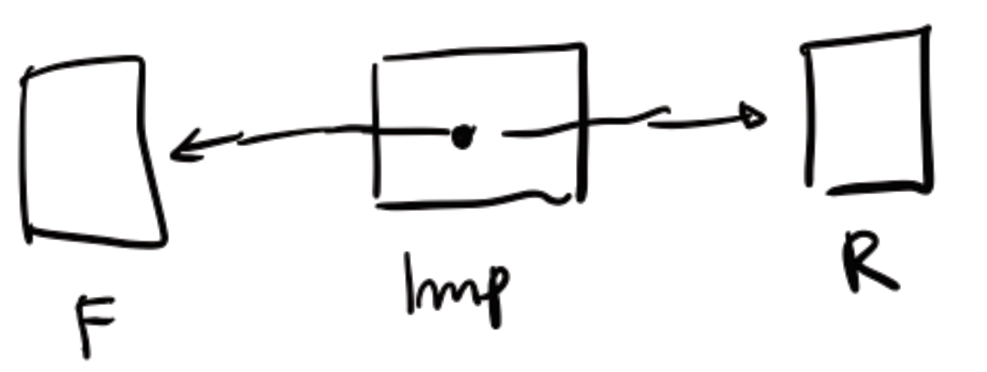
\includegraphics[scale=0.33]{dpcatfig_fir}
    \caption{\label{fig:FIR}}
\end{figure}


% \paragraph{Preference / utility}
%
% Both functionality and resources are ordered sets. In fact, the functional
% requirements are usually specified as lower bounds, and the resource
% constraints are specified as upper bounds.


\paragraph{Systems and components}

Engineers tend to approach complex design problems hierarchically.  The usual
nomenclature refers to \textit{systems} being decomposed into \textit{components}.

What is a system, and what is a component? Here is a great quote:

\begin{quote}
A system is composed of components; \\
a component is something you understand.\\
---Howard Aiken\footnote{
Howard H. Aiken (1900-1973), creator of the MARK I computer.
Quoted by Kenneth E. Iverson (1920-2004), creator of programming language APL.
Quoted in this paper\cite{that-paper},
  but ultimately sourceless and probably apocryphal.}
\end{quote}

The first part of the quote, "A system is composed of components", is plain as day as much as
it is tautological. We could equally say: "A system is partitioned in parts".

The second part, "a component is something you understand", is the insightful part: We call
"system" what is not obvious to understand, even if we understand all its components
separately.

Whether something can be considered a component, an indivisible atom in the theory, depends on the context.
%
% This definition is, of course, an anthropocentric definition, as it is a
% limitation of the human mind, related to the amount of neurons in the brain. It
% also depends on what exactly is the task at hand with which we are confronted.


\paragraph{Interfaces and interconnection}

Components are \emph{interconnected} to create a system.
This implies that we have defined the \emph{interfaces} of components, which
have the dual function of delimiting when one component ends and another begins,
and also to describe exactly what is the nature of their interaction.

\begin{example}
    \todo{Dynamical systems}
\end{example}

\begin{example}
    \todo{Energy exchange}
\end{example}

In this paper, we will present a formalism in which the functionality and resources
are the interfaces used for interconnection: Two components are connected
if the resources required by the first correspond to the functionality
provided by the second.
%
% Pictorially, the situation is as in \cref{fig:FIRFIR}.
%
% \begin{figure}[h!]
%     \todo{F-I-R-F-I-R}
%     \caption{\label{fig:FIRFIR}}
% \end{figure}

\AC{add example}
\GZ{Question: Could we take one of the easy examples in your paper?}


\paragraph{Abstraction}

By \emph{abstraction}, one usually means that it is possible to ``zoom out'',
in the sense that a system of components can be seen as a component itself,
which can be part of larger systems.

\todo{Say something about systems of systems}


\paragraph{Compositionality}

A \emph{compositional} property is a property that is preserved by interconnection and abstraction; assuming each component in a system satisfies that property, also the system as a whole satisfies the property.

\begin{example}
One can compose two electronic circuits by joining their terminals to obtain
another electronic circuit. We would say that the property
of being an electronic circuit is compositional.
% However, in general the dynamics
% of the two circuits could be arbitrarely different if the
\end{example}



\paragraph{Design Queries}

\AC{Introduce the 3/4 usual queries}



%\begin{example}
%Let's consider a linear time-invariant system
%    \begin{equation*}
%    	\begin{align}
%    		\dot{x}_1(t) &= A_1x_1(t)+B_1u_1(t)\\
%    		y_1(t)&=C_1x_1(t)+D_1u_1(t),
%    	\end{align}
%    \end{equation*}
%    where $u_1(t)$ represents the input of the system and $y_1(t)$ represents its output. If we now consider a second linear time-invariant system which has as input the output of the first linear system, we can write it as
%    \begin{equation*}
%    	\begin{align}
%    		\dot{x}_2(t)&=A_2x_2(t)+B_2C_1x_1(t)+B_2D_1u_1(t)\\
%    		y_2(t)&=C_2x_2(t)+D_2C_1x_1(t)+D_2D_1u_1(t).
%    	\end{align}
%    \end{equation*}
%    These two systems can be re-written into a single system, which turns out to be linear time-invariant as well:
%    \begin{equation*}
%    \begin{align}
%    	\begin{bmatrix}
%    	\dot{x}_1(t)\\
%    	\dot{x}_2(t)	
%    	\end{bmatrix}&=
%    	\begin{bmatrix}
%    	A_1&0\\
%    	B_2C_1&A_2
%    	\end{bmatrix}\begin{bmatrix}
%    	x_1(t)\\
%    	x_2(t)
%    	\end{bmatrix}+
%    	\begin{bmatrix}
%    		B_1\\
%    		B_2D_1
%    	\end{bmatrix}u_1(t)\\
%    	\begin{bmatrix}
%    	y_1(t)\\
%    	y_2(t)	
%    	\end{bmatrix}&=\begin{bmatrix}
%    	C_1&0\\
%    	D_2C_1&C_2
%    	\end{bmatrix} \begin{bmatrix}
%    	x_1(t)\\
%    	x_2(t)
%    	\end{bmatrix} + 
%    	\begin{bmatrix}
%    		D_1\\
%    		D_2D_1
%    	\end{bmatrix}u_1(t).
%    \end{align}
%    \end{equation*}
%
%\end{example}

\todo{check commented example}

%
% In Censi's theory, one considers ``design problems''
% as relations between ``resources''---such as batteries, motors, robots, etc.

%
% \begin{compactitem}
%     \item a notion of ``resources''
%     \item a notion of ``resource transformation'' (how one resource can be turned into another);
%     \item a notion of composition (vertical and horizontal composition);
%     \item and a notion of utility: one object may be more useful in the design space than another.
% \end{compactitem}
%
% We will see that category theory provides a great way to describe all this
% notions together in a clear framework.


\subsection{Queries in design}
\AC{Describe here the queries}





\clearpage
% DP Traced monoidal
% !TEX root = ../CategoricalCoDesign.tex
\subsection{to put back up}


\begin{figure}[h!]
\centering
\begin{subfigure}{0.2\textwidth}
\centering
\includesag{50_sum_series}
\caption{Series: $(f \then g)$.}
\end{subfigure}
\hspace{10mm} % add space between figures
\begin{subfigure}{0.2\textwidth}
\centering
\includesag{50_sum_parallel}
\caption{Parallel: $f \otimes g$.}
\end{subfigure}
\hspace{10mm} % add space between figures
\begin{subfigure}{0.2\textwidth}
\centering
\includesag{50_sum_biproduct}
\caption{Biproduct: $f + g$.}
\end{subfigure}
\hspace{10mm} % add space between figures
\begin{subfigure}{0.2\textwidth}
\centering
\includesag{50_sum_loop}
\caption{Loop: $\Tr f$.}
\end{subfigure}
\label{fig:diagrams}
\end{figure}

\begin{table}[t!]
    \centering
\begin{tabular}{c|c|c|crl}
    series &
    $f:A\tickar B$&
    $g:B\tickar C$&
    $f\then g:$&$A$&$\tickar C$ \\
    %
    sum &
    $f:A\tickar B$ &
    $g:A\tickar B$ &
    $f\vee g:$&$A$&$\tickar B$ \\
    %
    intersection &
    $f:A\tickar B$ &
    $g:A\tickar B$ &
    $f\wedge g:$&$A$&$\tickar B$ \\
    %
    monoidal product &
    $f:A\tickar C$&
    $g:B\tickar D$ &
    $f\otimes g:$&$A\times B$&$\tickar C \times D$ \\
    %
    product &
    $f:A\tickar C$&
    $g:A\tickar D$ &
    $f\times g:$&$A $&$\tickar C + D$ \\
    %
    coproduct &
    $f:A\tickar C$&
    $g:B\tickar C$ &
    $f\sqcup g:$&$A + B $&$\tickar C$ \\
    %
    biproduct &
    $f:A\tickar B$ &
    $g:A\tickar B$ &
    $f+ g:$&$A + A$&$\tickar B + B$ \\
    %
    trace &
    $f: C \times A \tickar C \times B$ &
    -&
    $\Tr_{A,B}^C(f) :$&$A$&$\tickar B$
\end{tabular}
    \caption{Various composition operations on design problems (i.e. morphisms) in $\DP$.}
\end{table}
\clearpage
% Creating DPs
\include{chapters/60_creating_DPs}
\clearpage

\printbibliography

\end{document}
